% -*- Mode:TeX -*-

%% IMPORTANT: The official thesis specifications are available at:
%%            http://libraries.mit.edu/archives/thesis-specs/
%%
%%            Please verify your thesis' formatting and copyright
%%            assignment before submission. If you notice any
%%            discrepancies between these templates and the 
%%            MIT Libraries' specs, please let us know
%%            by e-mailing thesis@mit.edu

%% The documentclass options along with the pagestyle can be used to generate
%% a technical report, a draft copy, or a regular thesis. You may need to
%% re-specify the pagestyle after you \include cover.tex. For more
%% information, see the first few lines of mitthesis.cls. 

%\documentclass[12pt,vi,twoside]{mitthesis}
%%
%%  If you want your thesis copyright to you instead of MIT, use the
%%  ``vi'' option, as above.
%%
%\documentclass[12pt,twoside,leftblank]{mitthesis}
%%
%% If you want blank pages before new chapters to be labelled ``This
%% Page Intentionally Left Blank'', use the ``leftblank'' option, as
%% above. 

\documentclass[12pt,twoside]{mitthesis}
\usepackage{lgrind}
%% These have been added at the request of the MIT Libraries, because
%% some PDF conversions mess up the ligatures.  -LB, 1/22/2014
\usepackage{cmap}
\usepackage[T1]{fontenc}
\usepackage{slashed}
\usepackage[intoc]{nomencl}
\usepackage{cite}
\usepackage{braket}
\usepackage{url}

\usepackage{graphicx}
\usepackage{amsmath}

\usepackage{nomencl}

\usepackage{mathtools}

%\numberwithin{figure}{section}
%\numberwithin{table}{section}


\pagestyle{plain}

%% This bit allows you to either specify only the files which you wish to
%% process, or `all' to process all files which you \include.
%% Krishna Sethuraman (1990).

%\typein [\files]{Enter file names to process, (chap1,chap2 ...), or `all' to process all files:}
\def\all{all}
\ifx\files\all \typeout{Including all files.} \else %\typeout{Including only \files.} \includeonly{\files} \fi

\begin{document}

% -*-latex-*-
% 
% For questions, comments, concerns or complaints:
% thesis@mit.edu
% 
%
% $Log: cover.tex,v $
% Revision 1.9  2019/08/06 14:18:15  cmalin
% Replaced sample content with non-specific text.
%
% Revision 1.8  2008/05/13 15:02:15  jdreed
% Degree month is June, not May.  Added note about prevdegrees.
% Arthur Smith's title updated
%
% Revision 1.7  2001/02/08 18:53:16  boojum
% changed some \newpages to \cleardoublepages
%
% Revision 1.6  1999/10/21 14:49:31  boojum
% changed comment referring to documentstyle
%
% Revision 1.5  1999/10/21 14:39:04  boojum
% *** empty log message ***
%
% Revision 1.4  1997/04/18  17:54:10  othomas
% added page numbers on abstract and cover, and made 1 abstract
% page the default rather than 2.  (anne hunter tells me this
% is the new institute standard.)
%
% Revision 1.4  1997/04/18  17:54:10  othomas
% added page numbers on abstract and cover, and made 1 abstract
% page the default rather than 2.  (anne hunter tells me this
% is the new institute standard.)
%
% Revision 1.3  93/05/17  17:06:29  starflt
% Added acknowledgements section (suggested by tompalka)
% 
% Revision 1.2  92/04/22  13:13:13  epeisach
% Fixes for 1991 course 6 requirements
% Phrase "and to grant others the right to do so" has been added to 
% permission clause
% Second copy of abstract is not counted as separate pages so numbering works
% out
% 
% Revision 1.1  92/04/22  13:08:20  epeisach

% NOTE:
% These templates make an effort to conform to the MIT Thesis specifications,
% however the specifications can change. We recommend that you verify the
% layout of your title page with your thesis advisor and/or the MIT 
% Libraries before printing your final copy.
\title{Analysis of Beauty Quark Hadronization in Vacuum and Quark-Gluon Plasma with CMS}

\author{Zhaozhong Shi}

%\author{B. A., in Physics, University of California, Berkeley (2016)}

\prevdegrees{B.A., University of California, Berkeley (2016)}

% If you wish to list your previous degrees on the cover page, use the 
% previous degrees command:
%       \prevdegrees{A.A., Harvard University (1985)}
% You can use the \\ command to list multiple previous degrees
%       \prevdegrees{B.S., University of California (1978) \\
%                    S.M., Massachusetts Institute of Technology (1981)}
\department{Department of Physics}

% If the thesis is for two degrees simultaneously, list them both
% separated by \and like this:
% \degree{Doctor of Philosophy \and Master of Science}
\degree{Doctor of Philosophy in Physics}

% As of the 2007-08 academic year, valid degree months are September, 
% February, or June.  The default is June.
\degreemonth{September}
\degreeyear{2021}
\thesisdate{September 5, 2021}

%% By default, the thesis will be copyrighted to MIT.  If you need to copyright
%% the thesis to yourself, just specify the `vi' documentclass option.  If for
%% some reason you want to exactly specify the copyright notice text, you can
%% use the \copyrightnoticetext command.  
%\copyrightnoticetext{\copyright IBM, 1990.  Do not open till Xmas.}

% If there is more than one supervisor, use the \supervisor command
% once for each.
\supervisor{Yen-Jie Lee}{Associate Professor}

% This is the department committee chairman, not the thesis committee
% chairman.  You should replace this with your Department's Committee
% Chairman.
\chairman{Nergis Mavalvala}{Associate Department Head of Physics}

% Make the titlepage based on the above information.  If you need
% something special and can't use the standard form, you can specify
% the exact text of the titlepage yourself.  Put it in a titlepage
% environment and leave blank lines where you want vertical space.
% The spaces will be adjusted to fill the entire page.  The dotted
% lines for the signatures are made with the \signature command.
\maketitle

% The abstractpage environment sets up everything on the page except
% the text itself.  The title and other header material are put at the
% top of the page, and the supervisors are listed at the bottom.  A
% new page is begun both before and after.  Of course, an abstract may
% be more than one page itself.  If you need more control over the
% format of the page, you can use the abstract environment, which puts
% the word "Abstract" at the beginning and single spaces its text.

%% You can either \input (*not* \include) your abstract file, or you can put
%% the text of the abstract directly between the \begin{abstractpage} and
%% \end{abstractpage} commands.

% First copy: start a new page, and save the page number.
\cleardoublepage
% Uncomment the next line if you do NOT want a page number on your
% abstract and acknowledgments pages.
% \pagestyle{empty}
\setcounter{savepage}{\thepage}
\begin{abstractpage}
% $Log: abstract.tex,v $
% Revision 1.1  93/05/14  14:56:25  starflt
% Initial revision
% 
% Revision 1.1  90/05/04  10:41:01  lwvanels
% Initial revision
% 
%
%% The text of your abstract and nothing else (other than comments) goes here.
%% It will be single-spaced and the rest of the text that is supposed to go on
%% the abstract page will be generated by the abstractpage environment.  This
%% file should be \input (not \include 'd) from cover.tex.
An analysis of fully reconstructed $B^0_s$ and $B^+$ mesons decay into $J/\psi$ and strange hadrons using Compact Muon Solenoid (CMS) Experiment 2017 pp dataset and 2018 PbPb data at the center of mass energy per nucleon $\sqrt{s_{NN}} = 5.02$ TeV at the Large Hadron Collider (LHC) is presented. We apply machine learning techniques along with multivariate analysis to obtain significant B-meson signals and extend the kinematic regime of B-meson measurements with higher precision. In our analysis, $B^0_s$ signal of greater than 5 $\sigma$ significance is observed for the first time in heavy-ion collisions. The measured $B^0_s$/$B^+$ ratio in PbPb along with pp references are compared with theoretical model predictions. These results will help elucidate the beauty quark hadronizaton mechanisms in vacuum and quark-gluon plasma at the LHC energy. Significant B-meson signals have also been observed at low very $p_T$ and high multiplicity in pp collisions, which will allow us study beauty hadrochemistry in small systems and energy loss mechanism in the future. 
\end{abstractpage}

% Additional copy: start a new page, and reset the page number.  This way,
% the second copy of the abstract is not counted as separate pages.
% Uncomment the next 6 lines if you need two copies of the abstract
% page.
% \setcounter{page}{\thesavepage}
% \begin{abstractpage}
% % $Log: abstract.tex,v $
% Revision 1.1  93/05/14  14:56:25  starflt
% Initial revision
% 
% Revision 1.1  90/05/04  10:41:01  lwvanels
% Initial revision
% 
%
%% The text of your abstract and nothing else (other than comments) goes here.
%% It will be single-spaced and the rest of the text that is supposed to go on
%% the abstract page will be generated by the abstractpage environment.  This
%% file should be \input (not \include 'd) from cover.tex.
An analysis of fully reconstructed $B^0_s$ and $B^+$ mesons decay into $J/\psi$ and strange hadrons using Compact Muon Solenoid (CMS) Experiment 2017 pp dataset and 2018 PbPb data at the center of mass energy per nucleon $\sqrt{s_{NN}} = 5.02$ TeV at the Large Hadron Collider (LHC) is presented. We apply machine learning techniques along with multivariate analysis to obtain significant B-meson signals and extend the kinematic regime of B-meson measurements with higher precision. In our analysis, $B^0_s$ signal of greater than 5 $\sigma$ significance is observed for the first time in heavy-ion collisions. The measured $B^0_s$/$B^+$ ratio in PbPb along with pp references are compared with theoretical model predictions. These results will help elucidate the beauty quark hadronizaton mechanisms in vacuum and quark-gluon plasma at the LHC energy. Significant B-meson signals have also been observed at low very $p_T$ and high multiplicity in pp collisions, which will allow us study beauty hadrochemistry in small systems and energy loss mechanism in the future. 
% \end{abstractpage}

\cleardoublepage

\section*{Acknowledgments}

%This is the acknowledgements section. You should replace this with your own acknowledgements.

Today, sitting in front of my Macbook and writing up my PhD thesis, I am recalling the nice memory over the past 5 years of my academic and research journey at MIT. I have overcome countless challenges and seized every opportunity. I have absorbed plenty of knowledge like nutrients and lead work alcoholic life. I used to work more than many hours, particularly when deadlines are approaching. I am glad that I have overcome countless of deadlines and managed to finish most of my tasks on time during my graduate studies. Because of my hard work and achievements, during my graduate studies at MIT, I have been awarded the NSF-GRFP and DOE SCGSR fellowships. While I am proud of my academic and research accomplishments, the more importance things are love and friendship. I have been to many memorable places around the world and met many interesting people. They have taught me more than I can learn from papers, lectures, and experiments. I owed them a lot and am indebted to everyone for their influences on me. Without them, I will not be able to finish this work and reach my current maturity.

On the cloudy afternoon of February 12, 2016, I was anxiously waiting for my graduate admission decisions. At around 2pm when I am returning home from Berkeley, I received my acceptance to MIT from the MIT Department of Physics Coordinator Catherine Modica. At that moment, I was still on my BART from UC Berkeley back to San Francisco. I was very excited and immediately called my family to share this great news. I understood that this would be the start of my exciting career as a PhD candidate in Nuclear Physics research. Without thinking too much, I quickly accepted the offer and got ready to join MIT.

During the MIT Open House, I met a lot of amazing people. I first visited the MIT Heavy Ion Group and then made friends with many of my peers. I would really like to thank Constantin Weisser for his generous accommodation during the Open House. I met my future PhD advisor Professor Yen-Jie Lee and LNS director Bolek Wyslouch. I also met my fellow students at LNS such as Lauren Yates, Sangbaek Lee, and Yi Jia. They are all very nice and kind. We have spent our first three semesters together taking classes and discussing physics. Particularly, I want to mention Sangbaek that we used to discuss a lot about our life stories and future perspectives together. It was a quite memorable experience. I also frequently visited lattice QCD theorist Anthony Grebe. I still remembered the time we discussed physics questions, debated ideas, derive formulae at the Center for Theoretical Physics. He is a truly humble and kind person. I wish him to have a successful future career in theoretical particle physics.


As a resident of MIT Tang Hall, I met many interesting people. Here, I would like to thank Ali Fahimniya who also lived at Tang Hall for his first year. We often chat with each other during the cookies social in the Pappalardo Room. We shared our life experience and future plan. It turns out that we defended our PhD just a day apart from each other. 

Shortly after attending MIT, I decided to join the MIT Heavy Ion Group and pursued my scientific research career in Experimental High Energy Nuclear Physics as my PhD thesis topic for the next 5 years. Members of the MIT Heavy Ion Group have provided me with general supports and comprehensive guidance towards my PhD. Without them, I would not be able to overcome challenges and finish my thesis research projects. 


At the graduate student's office, my desk is located in the northwest corner. Senior members of faculties in our group offered me excellent training and many opportunities to become an independent researcher and build up my international reputation in the field. I would particularly like to thank Professor Yen-Jie Lee for his long and enduring support, both in research and life, for the past 5 years. He has provided me with many opportunities and ideas to carry out physics analysis and fought in the CMS collaboration to allow me to give talks in internationally recognized conferences. I am also deeply indebted to him for his care of my career development and letters of recommendation for fellowships and postdoctoral scholar positions. Thanks to his nurture, I have transformed from a student knowing almost nothing to become an independent researcher with some big-picture visions. I am also grateful to the MIT Heavy Ion Group leader Professor Gunther Roland for his generous supports to allow me to work on sPHENIX and EIC projects. His letters of recommendation and grant management advice helps me a lot to get my first postdoctoral position and become professional in developing leadership skills in academia. Both of them have provided me with opportunities to work at different places around the world such as MIT, Fermilab, BNL, and CERN. Aside from them, I appreciated the general academic etiquette and soft skills from Professor Bolek Wyslouch.


My fellow senior graduate colleagues in my group have influenced me a lot. First, the most senior graduate student Dragos Velicanus showed me around about our group and guided me through the basics. He also provided a lot of remarks on my fellowship applications. Then, Alex Barberi sat next to my office desk. We have worked together and talked about funny anecdotes. I also made acquittances with Ta-Wei Wang. He created the skimmed files for me to play with and answered me many technical questions in C$++$ programming and B mesons full reconstructions. As a newbie in the CMS analysis, I used to frequently bother Jing Wang in the analysis techniques and questions on codes. However, she still patiently guided and helped me until my confusion was gone. As the CMS spectra heavy flavor group leader, she also gave a lot of feedback and suggestions to validate the analyses. Ran Bi, whose research was on photon-jet studies, was a bit reserved but still kindly helped me a lot with CMS software and technical concepts for data processing and analysis. Kaya Tatar was a very nice and resourceful person. We used to discuss many physics and technical questions. Chris McGinn was one of my best friends at the MIT Heavy Ion Group. He provided me with a lot of technical assistance and helped me debug my codes. His help was very effective. I really appreciated that. We also debated many physics concepts and politics issues. Austin Baty was one of my buddies at CERN who used to share his experience in life and studies with me.  

Junior graduate students such as Michael Peters, Molly Taylor, and Gwang-Jun Kim were all very friendly and kind. I will never forget the time when Michael and I initiated the debate and keep on our position to try to convince with each other. I also enjoyed working with Gwang-Jun and still remember the moments we stay up many days and nights fighting to get the analysis from pre-approve to approval stage. I also would like to thank Molly for helping me look after my remaining items near my desks in the MIT office since I went to CERN. 


Staff members of our group were very professional and resourceful. Dr. Gian Michele guided me through my analysis and gave me useful feedback for my first Quark Matter talk. I have learned a lot from him in the first two years of my PhD studies. Dr. Camellia Mironov has guided me through the CMS collaboration bureaucracy and went through the procedures to present and publish papers. Dr. George Stephans has provided me with many suggestions in MC simulations, technical questions, physics concepts, and computing knowledge. Dr. Christoph Roland has shared me with a lot of heavy-ion physics anecdotes, career development stories, detector hardware knowledge, software development skills, and analysis techniques. I would also like to thank Dr. Ivan Cali for his suggestions in windows codes programming, software development, and product design. Finally, I would like to thank the administrative assistant Anna Convertino for handling my travel and paperwork.  

%Faculty Yen-Jie; emphasize. 

I would also like to thank my fellow students at the PPC including Dr. Dylan Hsu, Dr. Brandon Allen, Dr. Sid Narayanan, Dr. Stephanie Brandt, and Jeff Krupa. They are all my good friends. We treated each other like brothers and made fun of each other. I still remembered I visited the PPC office almost every day and shared how my day was with them. They used to say I would not be able to graduate in 6 years but I did manage to get my PhD within 5 years, which surprised them a lot. Jeff was also my buddy. We used to go out for lunch regularly and walked along the beach every semester. I missed them all very much!

Aside from that, many other professors at MIT have helped me a lot academically and professionally. I would particularly thank my academic advisor Professor Lindley Winslow. She is very kind, considerate, and helpful. She gave me very good advice on fellowship applications, courses selections, degree preparation, and postdoc tips. My graduate career has become much smoother and planned thanks to her kind suggestions. In addition, I would like to thank Professor Iain Stewart, Richard Milner, and Krishna Rajagopal for occasional discussions. I would also like to thank Professor Barton Zwiebach for serving as the reader in my PhD thesis committee and provided me with some useful feedback about my defense and presentation.

Outside MIT, I have also met many senior sages who have given me a lot of wisdom. As a member of sPHENIX calorimetry test beam crews at Fermilab, I met Dr. Craig Woody and worked with him during the first days in 2017. After that, he has been my mentor for the past 5 years and served as my laboratory scientist for the Electron-Ion Collider Electromagnetic Calorimeter project in my DOE SCGSR award. Moreover, he has written many letters for me and provided me with a lot of resources for career development. I am very thankful for his support. I also met Dr. Jin Huang and received many technical and analysis guidances for my sPHENIX EMCAL, heavy flavor simulation, and EIC EMCAL projects. I would also like to thank Dr. John Haggerty for his creative training during my shift at Fermilab in 2017 and 2018. At CERN, I felt very fortunate to work with Professor Mario Sitta on ALICE ITS project. He was my best friend during my stay in France and has kindly helped me move my personal items around with his car and debug my programs. Without him, my stay at CERN could be very miserable. I would also like to express my sincere gratitude to my collaborator Nuno Leonardo at LIP in Portugal. Collaborating on the B-meson analysis, he has provided me with many concrete solutions to improve the analysis, ideas to overcome the challenges from the CMS collaboration, and workforce supports to complete part of the projects. He has saved this analysis many times. His efforts, along with my hard work, finally managed to make it possible and become part of my thesis. Without his support, my analysis would be stuck in many steps and may not be able to advance to the current ready for submission stage. His urgent emails and slack messages were still clearly remembered in my mind. I also met Ming Liu during the Fermilab test beam shift and ALICE ITS commissioning at CERN. We worked together at that time. We will work together as a postdoc and a mentor for the next three years. Finally, I am very lucky to have a chance to have a nice lunch with Professor James Bjorken. I have really learned many stories in the great old days of the Golden Age of particle physics and about the fun of physics with him. I also got to know his recent research interests and received some career advice from him. It was my great honor to chat with this great mind.

In addition to my mentors, colleagues, and friends, I would also like to thank my family. During the COVID-19 pandemic in the last year of my PhD studies, I stayed at home and received a lot of care from them. I was able to really focus on finishing my thesis research and became much more productive than in the past 3 years. I am really grateful to their unconditional love. 

Finally, I would really like to especially thank my significant other Zhixin Lai in this paragraph. Since I met her in February 2020, she has been my soul mate. We shared everything in our life, worked together, and have learned a lot from each other. When we experienced obstacles and failures, we cheered each other up. When we saw opportunities and success, we expressed our happiness with each other and celebrated our achievements on the phone. She has helped me a lot in my career and gave me many helpful suggestions to improve the writing of my fellowship applications, job hunting, and PhD thesis. After almost a year and a half since we knew each other, the US-Canadian border was finally open. I finally had a chance to meet her in person. We sat together and prepared my thesis defense. Her company with me in my PhD thesis defense and my celebration dinner made it the most memorable day in my life. She has made me a more complete and mature person. I am indebted to her sincere love and really hope to experience more ups and downs with her in the future.



%BNL: Craig Woody. Jin Huang. John Haggerty.

%LANL: ming

%Fermilab:

%SLAC: BJ


%CERN: Marrio Sitta, Ivan, Markus Keil, 



%I lived at Tang Hall and met many amazing people 


%Grad Lounge guys,

%PGSC Pizza social guys

%PPC bros

%MIT Heavy Ion group members



I am sorry that I may not be able to exhaust the list of everyone. But I really believe that I have learned a lot from all of you. I am sincerely grateful to your influences and friendships on my growth as a scientist and a person. 

%%%%%%%%%%%%%%%%%%%%%%%%%%%%%%%%%%%%%%%%%%%%%%%%%%%%%%%%%%%%%%%%%%%%%%
% -*-latex-*-

% Some departments (e.g. 5) require an additional signature page.  See
% signature.tex for more information and uncomment the following line if
% applicable.
% % -*- Mode:TeX -*-
%
% Some departments (e.g. Chemistry) require an additional cover page
% with signatures of the thesis committee.  Please check with your
% thesis advisor or other appropriate person to determine if such a 
% page is required for your thesis.  
%
% If you choose not to use the "titlepage" environment, a \newpage
% commands, and several \vspace{\fill} commands may be necessary to
% achieve the required spacing.  The \signature command is defined in
% the "mitthesis" class
%
% The following sample appears courtesy of Ben Kaduk <kaduk@mit.edu> and
% was used in his June 2012 doctoral thesis in Chemistry. 

\begin{titlepage}
\begin{large}
This doctoral thesis has been examined by a Committee of the Department
of Chemistry as follows:

\signature{Professor Jianshu Cao}{Chairman, Thesis Committee \\
   Professor of Chemistry}

\signature{Professor Troy Van Voorhis}{Thesis Supervisor \\
   Associate Professor of Chemistry}

\signature{Professor Robert W. Field}{Member, Thesis Committee \\
   Haslam and Dewey Professor of Chemistry}
\end{large}
\end{titlepage}


\pagestyle{plain}
  % -*- Mode:TeX -*-
%% This file simply contains the commands that actually generate the table of
%% contents and lists of figures and tables.  You can omit any or all of
%% these files by simply taking out the appropriate command.  For more
%% information on these files, see appendix C.3.3 of the LaTeX manual. 
\tableofcontents
\newpage
\listoffigures
\newpage
\listoftables

%% This is an example first chapter.  You should put chapter/appendix that you
%% write into a separate file, and add a line \include{yourfilename} to
%% main.tex, where `yourfilename.tex' is the name of the chapter/appendix file.
%% You can process specific files by typing their names in at the 
%% \files=
%% prompt when you run the file main.tex through LaTeX.
\chapter{Introduction}

\section{The Standard Model of Particle Physics}

%Physics is the research of relationship between space and time and energy and matter. Physicists enjoy searching for symmetries and consideration laws in nature. They develop elegant mathematical formulations to describe the beauty of the nature and predict or explain the experimental results and observed phenomena. 

There are four known fundamental forces in nature: gravitational force, electromagnetic force, strong force, and weak force. The gravitation force describes the interaction between two massive objects. The electromagnetic force describes the interaction between electrically charged objects. The strong force describes the interaction between nucleons. The weak force describe the radioactive decay of particles. The Standard Model (SM) of Particle Physics, first proposed and named by physicist Steven Weinberg in the 1960s \cite{StandardModel}, is based on theoretical frame of relativistic quantum field theory with a gauge symmetry of $SU(3) \times SU(2) \times U(1)$ \cite{SMTheory}. It unifies the electromagnetic and weak interactions and include the strong interaction into a theory and describes all particles participating in these interactions. The ingredient of the standard model are leptons, quarks, gauge bosons, and the Higgs boson shown in Figure~\ref{fig:SMParticle}.

\begin{figure}[hbtp]
\begin{center}
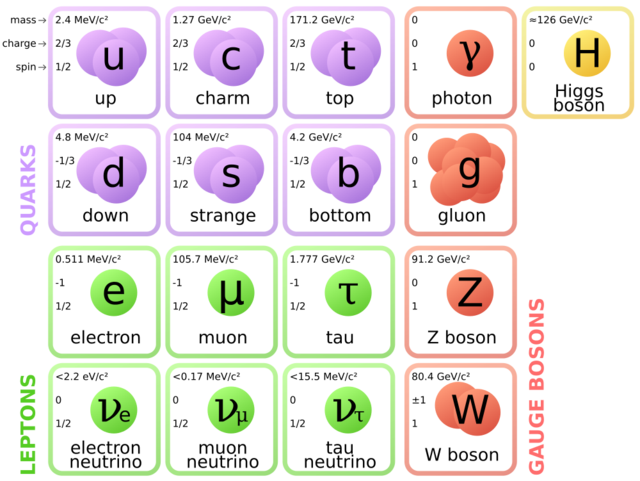
\includegraphics[width=0.50\textwidth]{Figures/Chapter1/SMParticles.png}
\caption{The 17 elementary particles, including 6 leptons, 6 quarks, 4 gauge bosons, and the Higgs boson, and their basic properties, such as mass, electric charge, spin, in the Standard Model of Particles Physics are shown above.}
\label{fig:SMParticle}
\end{center}
\end{figure} 


There are 19 parameters in the Standard Model: 6 quark masses, 3 lepton masses, 3 coupling strengths, 4 angles in the Cabibbo?Kobayashi?Maskawa Matrix, Higgs mass, vacuum expectation value, and QCD vacuum angle. These parameters are determined from the experiments. Physicists perform calculations based on the Standard Model and predict the cross section of different processes in high energy physics experiments. Since it is proposed in the 1970s, the Standard Model has been tested extensively in countless high-energy physics experiments. Its prediction holds for all of them with very few exceptions. The Standard Model consists of two sectors: the Electroweak theory (EW) and Quantum Chromodynamics (QCD). The Lagrangian of the Standard Model can be written as the sum of EW and QCD: $\mathcal{L_{SM}} = \mathcal{L_{EW}} + \mathcal{L_{QCD}}$ 


\section{Quantum Chromodynamics}

\subsection{QCD Lagrangian}

QCD, a non-abelian gauge theory with $SU(3)$ symmetry, is the theory for the strong interaction between quarks and gluons. The QCD Lagrangian is shown as follows:


\begin{equation}
\mathcal{L_{QCD}} = \bar \Psi^i i (\slashed{D})_{ij} \Psi^j - m  \bar \Psi^i \Psi_i - \frac{1}{16\pi^2} G^{\mu\nu}_{a}G_{\mu\nu}^{a}
\end{equation}

Where 

\begin{equation}
\slashed{D} = \gamma^\mu \partial_\mu - i g_s \frac{\lambda}{2}  \gamma^\mu A_\mu
\end{equation}

\begin{equation}
G^{\mu\nu}_{a} = \partial^\mu A^\nu_{a} - \partial_{\nu} A^\mu_{a} + g_s f_{abc} A^\mu_b A^\nu_c 
\end{equation}

Here, $\lambda$ are the Gell-Mann Matrices. $f_{abc}$ is the structure of constant of $SU(3)$. $A^\mu$ is the eight gluon field. $g_s$ is the strong coupling constant. The color indices $i$ and $j$ run from 1 to 3, which stands for 3 colors: red, blue, and green. The gluon field indices $a$, $b$, and $c$ run from 1 to 8, standing for the 8 gluon state (Gluon octet as the combination of 3 color and 3 anticolor: $3 \times \bar 3 = 1 \oplus 8$) living in the adjoint representation of $SU(3)$ of color.  



\subsection{Asymptotic Freedom}

The running of the strong coupling constant $\alpha_s = \frac{g_s^2}{4\pi}$ according to the 1-loop calculations in the renomalization theory \cite{QCDRunning} is shown as follows

\begin{equation}
\alpha_{s} (Q^2) = \frac{12\pi}{(11 N_{c} - 2 N_{f}) \ln(\frac{Q^2}{\Lambda_{QCD}^2})}
\end{equation}

We can see that as the energy scale increases, the coupling strength of the strong interaction decreases. This is in contrast to QED where the electromagnetic coupling strength increases as the energy scale increases. In the ultra-violate limit $Q^2 \rightarrow \infty$ and $\alpha_{s} \rightarrow 0$, quarks and gluons behave like free particles. This feature in QCD is called Asymptotic Freedom \cite{QCDAsym}. Meanwhile, in the infrared limit, the strong coupling constant increases. Near the $\Lambda_{QCD} \simeq$100 MeV, the strong coupling is greater than 1, where the perturbative expansion of QCD breaks down. Experimentally, physicists measure the strong coupling constant at different energy scales from different experiments at different colliders. Figure~\ref{QCDCoupling} \cite{AlphaTheoEx} shows the running of strong coupling constant in experiment and comparison with the theoretical calculations 

\begin{figure}[hbtp]
\begin{center}
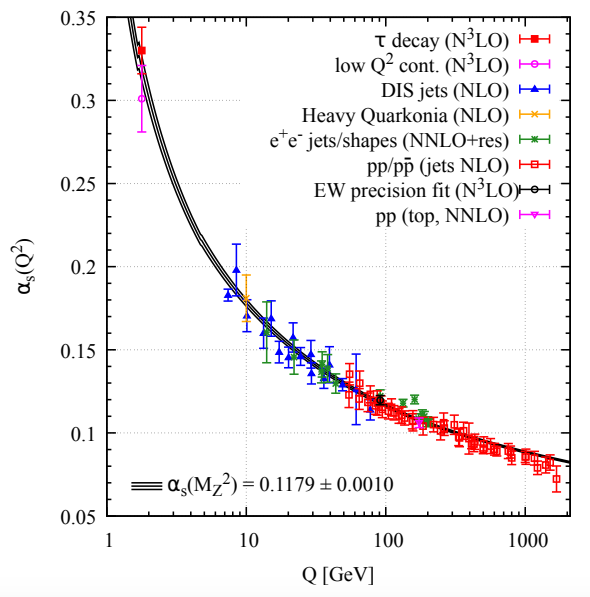
\includegraphics[width=0.50\textwidth]{Figures/Chapter1/QCDCoupling.png}
\caption{The running of the strong coupling constant $\alpha_s$ in different experiments at different energy scale $Q$ and the comparison with QCD calculations are shown above. Image from: \cite{AlphaTheoEx}}
\label{QCDCoupling}
\end{center}
\end{figure} 

An excellent agreement between theoretical predictions and experimental results of the strong coupling constant is observed in Figure~\ref{QCDCoupling}. 

\subsection{Perturbative QCD}

It is mathematically proven that there is in general no closed form expression for the partition function $Z[J(x)]$ Standard Model Lagrangian under the Quantum Field Theory framework.

\begin{equation}
Z[J(x)] = \int \mathcal{D}[\phi(x)] e^{iS + \int d^4 x J(x) \phi(x)}
\end{equation}

Therefore, physicists develop perturbation theory in Quantum Field Theory and apply it to the Standard Model. Physicist perform asymptotic expansions to obtain power series of the coupling constants and approximately calculate the expectation values of the observables to prediction experimental results.

For QCD, ,  perturbation theory is applicable to QCD in high energy and hard scattering processes since the coupling constant is much less than 1. Feynman rules and diagrams are applicable in the matrix element to evaluate the cross section of hard parton-parton scattering. Perturbative QCD (pQCD) calculations have been tested with various experiments such as electron-positron annihilations, deep inelastic electron-proton scatterings, and high energy proton-proton collisions.

\subsection{Non-perturbative QCD}

For soft scattering processes at low energy, the strong coupling constant is greater than 1. Perturbation theory of QCD breaks down. Many low-energy QCD processes such as hadronization and hadron-hadron interactions are non-perturbative. Historically, physicists developed Lattice gauge theory where the spacetime is discretized into lattice with finite size to evaluate the path integrals in the partition function $Z[J(x)]$. Lattice QCD can be applied to calculate the mass of the proton \cite{LQCDProtonMass}. Aside from Lattice gauge theory, effective theory is also to study non-perturbative QCD. For example, Chiral Perturbation Theory, where a low-energy effective Lagrangian in degree of freedom of hadrons is constructed by exploiting the approximate chiral symmetry while preserving other symmetries of parity and charge conjugation, has achieved some success to study pion-nucleon scattering \cite{ChiPT}. Non-perturbative QCD has achieved many successes in hadronic physics. Currently, some novel developments applying non-perturbative QCD to understand nuclear structure and nucleon spin structure are being carried by physicists. For instance, Chiral Perturbation Theory has been applied to study light nuclei structure such as ${}_{3}^{6}Li$ and ${}_{5}^{10}B$ \cite{ChiPTNuclear} and Lattice is employed to investigate nucleon spin structure \cite{LatticeNuclSpin}. 

\subsection{QCD Factorization Theorem}

The QCD factorization theorem states that in events with hadrons as incoming particle involving both hard and soft QCD processes, hard and soft process are mathematically factorized in the cross section computation shown schematically below \cite{QCDFactorization}: 

\begin{equation}
\sigma = PDF \otimes Diagrams \otimes FF
\end{equation}

\begin{figure}[hbtp]
\begin{center}
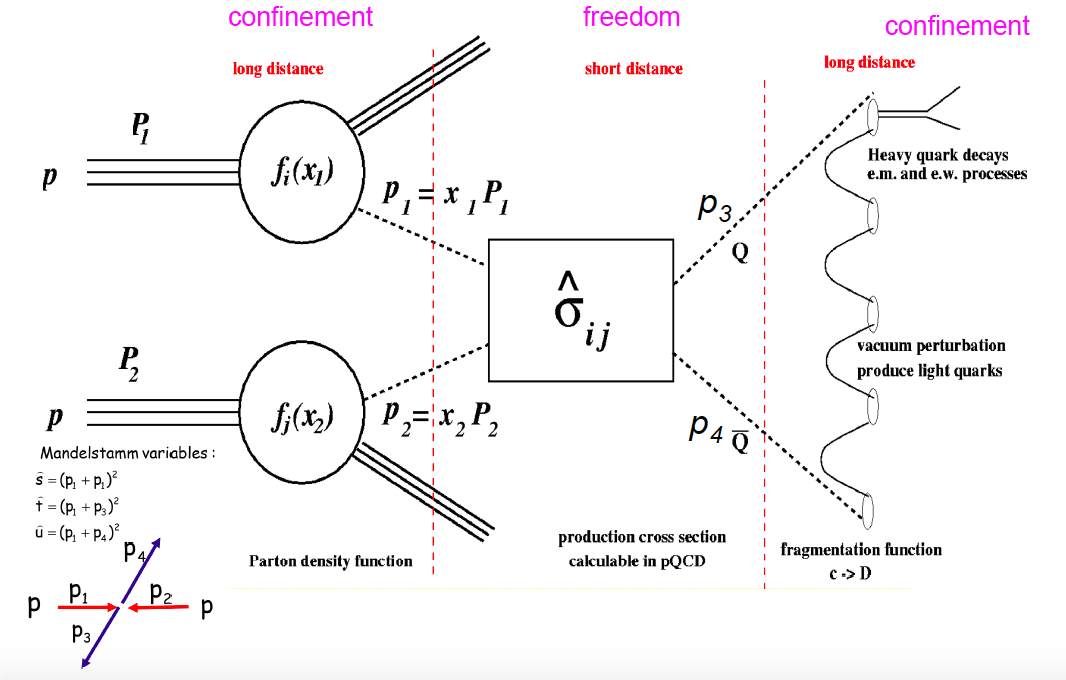
\includegraphics[width=0.75\textwidth]{Figures/Chapter1/QCDFactorizationTheorem.png}
\caption{The QCD factorization theorem applied to a pp collision event involving in soft and hard processes are shown above.}
\label{QCDFacTheo}
\end{center}
\end{figure} 

The hard processes are encoded in the factor of partonic cross sections while the soft processes are measured in experiments. Physicists employ parton distribution function (PDF), defined as the probability of finding a particle with a certain longitudinal momentum fraction $x$ at resolution scale of $\mu^2$, to describe the initial kinematic of partons inside hadrons \cite{PDFRef} and fragmentation function (FF), defined as the probability of a parton turn into a hadron $D_i^h(z)$ for a given energy fraction of the parton $z$ at resolution scale of $\mu^2$, to describe the hadronization process of partons \cite{QCDFFunc}. 

In addition to PDF, we could also define nuclear PDF (nPDF) for \cite{nPDF} to describe the parton kinematics inside nucleus. nPDF could be understood as the PDF of nucleons modified by the nuclear environment. Both parton distribution function and fragmentation function are extracted in experiments.

Physicists apply QCD factorization theorem to perform pQCD calculations and compare them with hadron spectra in electron-positron ($e^+e^-$), electron-proton ($ep$), and proton-proton ($pp$) collisions.

\subsection{Color Confinement}

Another feature of QCD as a non-abelian gauge theory is color confinement. The strong force carrier gluon itself is also color charged. Color charged partons, namely quarks and gluons, are never detected in isolation. In experiments, only color neutral hadrons are detected. Currently, the analytic explanation of color confinement is still not yet rigorously proven. The theoretical explanation of color confinement in QCD remains one of the unsolved problem in physics. 

\subsection{Hadronization}

The formation process hadrons from partons is called haronization. Because in experiments we can only measure final state hadrons, in order to study the interactions and dynamics of quarks and gluons during partonic stage from hadron spectra, we also need to understand hadronization mechanisms. However, hadronization is in general non-perturbative and cannot yet be described by first principle QCD calculations. Therefore, physicists make phenomenological models such as the Statistical Hadronization Model \cite{SHM}, Lund String Model \cite{LSM}, Cluster Hadronization Model \cite{CHM}, Quark Coalescence Model \cite{QCM} to study hadronization. Figure \ref{HadMech} schematically shows the hadronization of heavy quarks via fragmentation and recombination mechanism.

\begin{figure}[hbtp]
\begin{center}
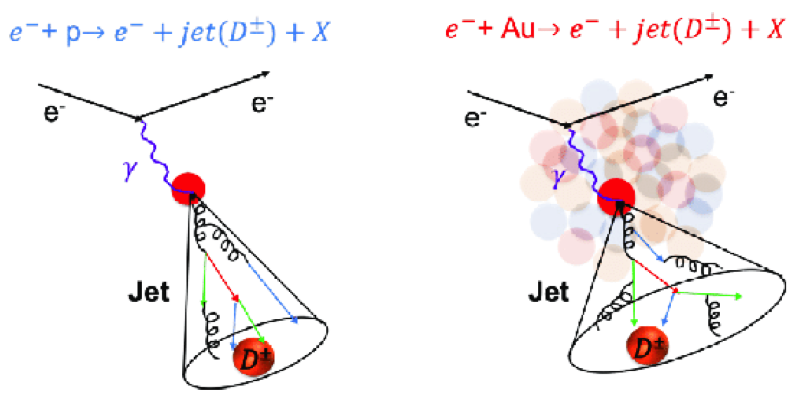
\includegraphics[width=0.48\textwidth]{Figures/Chapter1/FragCartoon.png}
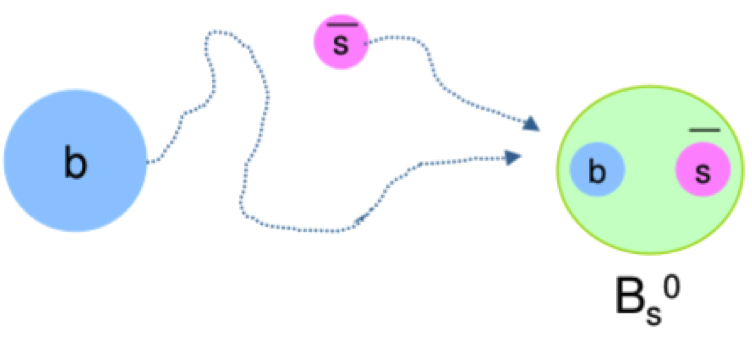
\includegraphics[width=0.48\textwidth]{Figures/Chapter1/CoalCartoon.png}
\caption{The fragmentation process of charms quarks hadronize into $D^\pm$ (left) and the coalescence process of beauty quark combining with a strange quark nearby to form a $B^0_s$ are shown above.}
\label{HadMech}
\end{center}
\end{figure} 


\subsection{Initial State and Final Effect}

In high energy proton-nucleus ($pA$) collisions, protons scatter off nucleons inside nuclei. Assuming QCD factorization still holds, nPDF could be applied to calculate the cross section of particle production. The initial state effects of nuclei including event-by-event geometry fluctuations due to nuclear dynamics \cite{GuntherV3}, nuclear shadowing effect \cite{IntroShadow}, EMC effect \cite{EMC} will modify the PDFs of nucleons in nuclei compare to PDFs of nucleons in vacuum. 

In the final state, the struck parton will lose energy from the interaction with the nuclear fragment and modify the final state hadron spectra. Because the parton-hadron interaction is generally non-perturbative, to retain the formula of QCD factorization theorem, the parton FF is modified \cite{CNEEFF}. These initial stage and final stage effects in $pA$ collision are call cold nuclear matter effects. 

\section{Hot QCD}

\iffalse 

\subsection{Initial State and Final Effect}


The development described in the previous section applies in small systems, for example, $e^+ e^-$, $ep$, and $pp$ collisions. In the smallest collision system $e^+e^-$, there is no initial state effect since the electron and positrons are point-like. In $ep$ and $pp$ collision, the initial state effects are encoded in the proton PDF. 

In high energy proton-nucleus collisions, proton scatter off nucleons inside nucleon. Assuming QCD factorization still applies, we can define nPDF to describe the kinematics of quarks inside nucleons of nucleus. We can see that there will be modification to the PDF for a nucleon vacuum due to the nucleon dynamics in the nuclei we can study the cold nuclear matter effect and probe the nPDF. In pA collisions, there many initial state effect depdendng on the collision $x$ and $Q^2$. For instance, we have nuclear shadowing, gluon saturation, and EMC effect. Both nPDF and the struck parton interact with the nuclear fragment will affect the final state hadron spectra. We call these effects in pA collision as cold nuclear matter effect.
%Hence, in addition to the initial state effect, there are also final state hot QCD matter effects in high energy nucleus-nucleus collisions.  

Initial state CGC 

\fi

\subsection{QCD in Finite Temperature} 

%In high energy, quarks and gluons inside nucleons of the nuclei become relevant to describe the event. As the energy increase, the quark and gluon density of the collision system increases. During the collisions, many quarks and gluons interact with each with in a small volume. 

In a system of dense and energetic quarks and gluons confined in a given size of volume, they scatter with each other and exchange momenta via the strong interaction. Many-body dynamics between quarks and gluons become relevant. In the limit of large number of quarks and gluons, after a sufficiently long period of time, the system eventually converges to the thermal equilibrium state via strong interaction \cite{MLBThermal,ADSCFTThermal,QCDThermal} regardless of its initial states. Therefore, a description based on thermodynamics can be formulated to study such systems \cite{QCDThemDyn}. We call this thermalized many-body system of quarks and gluons to be QCD matter. Therefore, a thermodynamic variable temperature ($\mathbf{T}$) can be introduced to characterize these many-body QCD systems. The study of many-body QCD in finite temperature is called hot QCD. 



\subsection{Temperature Dependence of QCD Static Potential}. 

If we consider two color charged quarks in the limit of infinite mass and are essentially at rest in the lab frame, we can define a QCD static potential between these two quarks due to the strong interaction. In vacuum, such a potential is called ``Cornell Potential'' \cite{Cornell}. The potential as a function of the distance between two quarks is shown as follows:

\begin{equation}
V(r) = -\frac{\alpha_{eff}}{r} + \sigma r
\end{equation}

Here, $\alpha_{eff}$ is the effective strong coupling coupling between the two quarks and $\sigma \simeq 0.184$ GeV/c is the string coupling constant \cite{CornellEquation}. 

Now if we consider a thermalized system in finite temperature $T$, the potential becomes: 

\begin{equation}
V(r) = -\frac{\alpha_{eff}}{r} e^{-m_D r} + \frac{\sigma}{m_D} (1 - e^{-m_D r})
\end{equation}

Here, $m_D \sim g_s T$ is the Debye mass due to Debye color screening effect \cite{CSEff}, which essentially modifies the gluon propagator by inserting a finite mass term: $-i \frac{g^{\mu\nu}}{q^2} \rightarrow -i \frac{g^{\mu\nu}}{q^2 - m_D^2}$. We have observed that as $V(\infty) = \frac{\sigma}{g_sT}$, which is finite for $T>$0. In fact, Equation (2) reduces to the Cornell potential when $T =$ 0. The QCD static potential is shown below in Figure~\ref{QCDPotential} \cite{TDepCornell}


\begin{figure}[hbtp]
\begin{center}
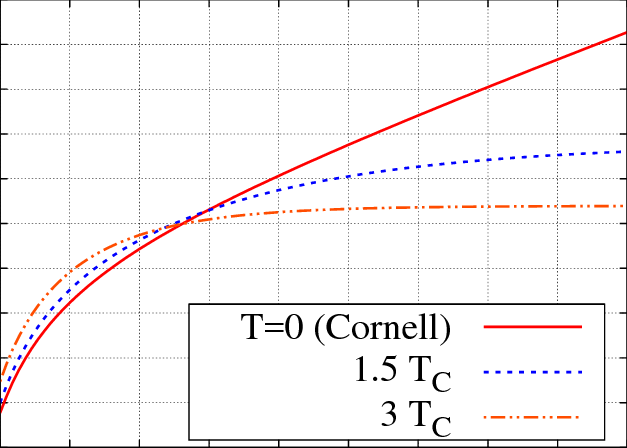
\includegraphics[width=0.55\textwidth]{Figures/Chapter1/QCDPotential.png}
\caption{The QCD potential $V(r)$ from at zero and at finite temperatures as a function of distance $r$ is shown above. Here, the critical temperature $T_c $ = 192 MeV. We can see that the QCD saturates at a finite value at finite temperature. }
\label{QCDPotential}
\end{center}
\end{figure} 


\subsection{Color Deconfinement}

As mentioned in the sections above, at finite temperature, the QCD static potential is screened and color degree of freedom become relevant in the system. As the temperature of the system increases, the quarks and gluon inside color-neutral hadrons will have more available space to move around and start to deconfine \cite{DeconfineTemp}. At some critical temperature $T_c$, quarks and gluons confined in hadrons will melt and form a new state of color deconfined QCD matter, which is called Quark-Gluon Plasma (QGP) \cite{QGPDeconfine}. The typical temperature of QGP is in the order of a few hundred MeV or about $10^{12}$ K, which is about hundreds of thousands times hotter than the core of the Sun. It is belived that QGP existed in the early universe several microsecond after the Big Bang \cite{}. Cosmologically, the study of QGP will help us understand the quark epoch and quark-hadron phase transition to under the history of the universe. 

%There are some interesting QCD phenomenologies involving temperature as listed in the following subsections.

%Hot applies in AA collision where a thermalized system is created. 

\subsection{QCD Phase Diagram}

Similar to form everyday matters such as metal, water, wood, glass, and plastic, which are formed by electromagnetic interaction and could all be described macroscopically by equations of states that are parameterized by thermodynamic variables. 
\iffalse Figure~\ref{QEDPhaseDiagram} shows the phase diagram of water ($\mathrm{H_2O}$) at different temperature and pressure:

\begin{figure}[hbtp]
\begin{center}
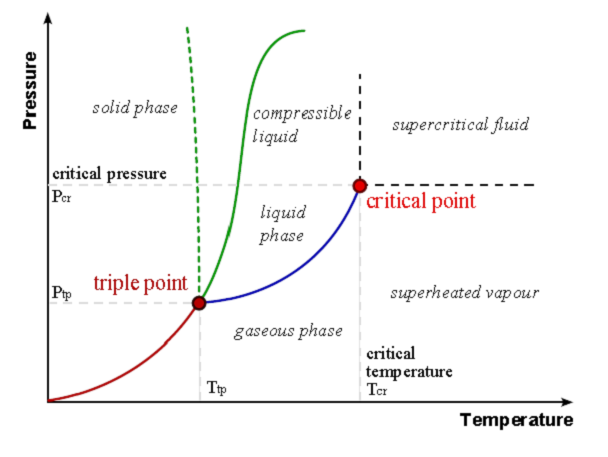
\includegraphics[width=0.45\textwidth]{Figures/Chapter1/WaterPhaseDiagram.png}
\caption{The P-T diagram of water in gas, liquid, solid phases is shown above.}
\label{QEDPhaseDiagram}
\end{center}
\end{figure} 

 
 \fi
Similarly, thermodynamical variables, for instance temperature ($\mathbf{T}$) and baryon chemical potential ($\mu_{B}$) can be introduced to characterize the equation of state of QCD matter formed via the strong interaction between many quarks and gluons. %Similarly, QCD matter is the matter formed by numerous quarks and gluons via the strong interaction and can also be describe by equations of states. L
Like our everyday matter which has gas, liquid, and solid phases at different pressure and temperature, QCD matter also has different phases at different temperature and baryon chemical potential. and can be describe by QCD phase diagrams. Figure~\ref{QCDPhaseDiagram} shows the QCD phase diagram at different temperature and baryon chemical potential:

\begin{figure}[hbtp]
\begin{center}
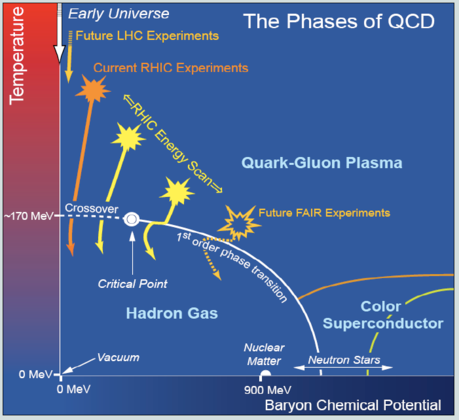
\includegraphics[width=0.60\textwidth]{Figures/Chapter1/QCDPhaseDiagram.png}
\caption{The theoretical QCD phase diagram of different QCD matter, including hadron resonance gas, quark-gluon plasma, neutron star, and color superconductor, as function of temperature and baryon chemical potential is shown above. The solid line indicates the conjecture of first order phase transition between quark-gluon plasma and hadron gas while the dash line is a smooth crossover. Thermodynamically, a critical points must exist in the boundary of smooth crossover and first order phase transition.}
\label{QCDPhaseDiagram}
\end{center}
\end{figure} 

We consider a system of free up and down quarks, antiquarks and gluons in temperature $T$ and baryon chemical potential $\mu_B$. According to MIT Bag Model \cite{MITBag}, its equation of state is given by

\begin{equation}
\epsilon(T,\mu_B) = \frac{37\pi^2}{30} T^4 + \frac{\mu_B^2}{3}T^2 + \frac{\mu_B^4}{54\pi^2} -  \mathcal{B}
\end{equation}

\iffalse
\begin{equation}
\epsilon(T,\mu_B) = \frac{37\pi^2}{30} T^4 + \frac{\mu_B^2}{7}T^2 + \frac{\mu_B^4}{161\pi^2} -  \mathcal{B}
\end{equation}
\fi

Here $p$ is the pressure and $\mathcal{B}$ is the bag constant, which can be understood as the pressure of the vacuum on the quarks and gluons to make them form hadrons with finite volume.

In a system of interacting quarks and gluons at $\mu_B=0$, based on lattice QCD calculations \cite{LatticeQGP}, the reduced energy density $\epsilon/T^4$ as a function of the temperature $T$ is shown below


\begin{figure}[hbtp]
\begin{center}
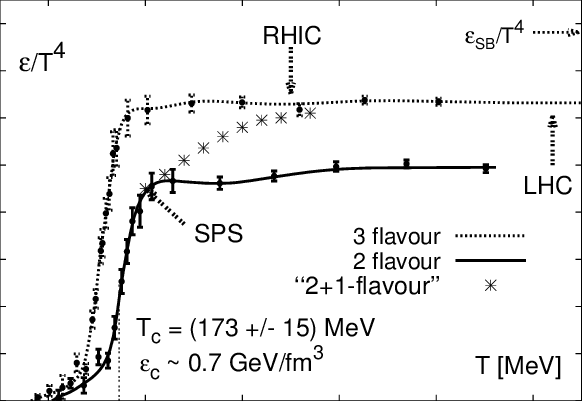
\includegraphics[width=0.60\textwidth]{Figures/Chapter1/LatticeData.png}
\caption{The reduced energy density $\epsilon/T^4$ as a function of temperature $T$ for different number of flavor scenarios from the lattice QCD calculations (data points) and the interpolation curves are shown above.}
\label{QCDPhaseDiagram}
\end{center}
\end{figure} 


A steep increase of the $\epsilon/T^4$ near the critical temperature at around $T_c  = 173$ MeV is observed, which signals the transition from hadron gas to the QGP \cite{PhaseTrans}. Experimentally, the critical point is estimated to be around $T_c = 175^{+1}_{-7}$ MeV and $\mu_B = (22 \pm 4.5)$ MeV \cite{CriticalPointEX} .






%Phase transition plot from LQCD

%Lattice QCD calculation has shown that.



%In the QCD phase diagram 

%Describe the diagram with QGP, Hadron Gas, and color superconductor.

%Talk a little about phase transition and critical point.

\section{High Energy Nuclear Physics}

Nuclear Physics is the study of atomic nuclei and their constituents and interactions. The typical energy scales of nuclear physics range from MeV to GeV. High Energy Nuclear Physics is a subfield of Nuclear Physics at an energy scale on the order of GeV. Its main goal is to under the physics of QCD matter from various approaches such as collider experiments, astrophysical observations, physics simulations, and theoretical modelings. In this thesis, I will focus on the research of QGP from the experimental approach using high energy heavy-ion colliders.

\subsection{Laboratories}

In laboratories, high energy nuclear physicists accelerate and collide heavy ions (A > 56) at center of mass high energy per nucleon at grater than 1 GeV to create extremely hot and dense conditions and study QGP. Relativistic heavy-ion collision is also known as ``The Little Bang'' compared to ``The Big Bang'' in cosmology \cite{LittleBang}. Historically, many colliders, such as the Alternating Gradient Synchrotron (AGS) at Brookhaven National Laboratory (BNL), in Upton, Long Island, New York and Super Proton Synchrotron (SPS) at European Center for Nuclear Research (CERN) in Meyrin, Switzerland, and GSI at Helmholtz Centre for Heavy Ion Research with both proton-proton and relativistic heavy-ion collision capabilities, have been built and established high-energy nuclear physics research programs. Today, two active colliders facilities, the Relativistic Heavy Ion Collider (RHIC) at BNL and the Large Hadron Collider (LHC) at CERN, are running at a wide range energies with various nuclei species and different impact parameters. In the future, another collider, called Facility for Antiproton and Ion Research (FAIR) running at relatively low energies, is being constructed at Darmstadt, Germany to map the location of the critical point in the QCD Phase Diagram. 

In addition to collider facilities, QGP might also be studied from astrophysical observations. For instance, strange stars, a quark star made of strange quark matter, may come from stable strangelet according to Bodmer--Witten conjecture \cite{SQMReview} or exist in the core of neutron stars under extreme pressure and temperature. It is believe there are several potential strange stars candidates according to telescope observations and gamma ray burst analysis \cite{SS1,SS2,SS3}.

%\subsection{Heavy-Ion Accelerators}

\subsection{Relativistic Heavy Ion Collider (RHIC)}

Located at BNL in Upton, Long Island, New York, United States of America, RHIC is one of the major high energy accelerator facilities and currently the highest energy collider in America. It is a circular collider with a circumference of 3.843 kilometers and can provide proton energy up to 500 GeV and gold ion energy up to 200 GeV \cite{RHICReport}. It was built in 2000 in order to search for a strongly interacting hot and dense state of nuclear matter created under ultra-relativistic heavy-ion collisions, currently known as QGP, with hints from the measurements at AGS and SPS. Moreover, RHIC provides physicists with a wide range of energies and a variety of ion species from proton to deuteron and cooper to uranium to create different sizes of systems at different temperature and baryon densities. In addition, taking the advantage of its highly polarization beam with high luminosity, RHIC has great machine capabilities for cold QCD physics. Figure \ref{RHIC} below shows a sky view of RHIC at BNL:


\begin{figure}[hbtp]
\begin{center}
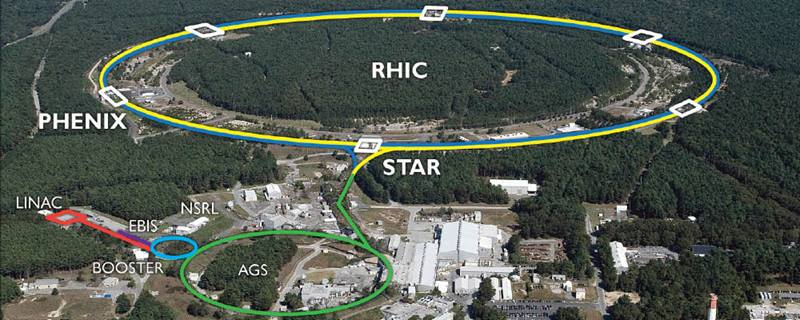
\includegraphics[width=0.85\textwidth]{Figures/Chapter1/RHIC.jpg}
\caption{The view of RHIC at BNL from the sky is shown above. The actual locations of other facilities at BNL, including Linac, Booster, EBIS, NSRL, AGS, and the experiments at RHIC such as, STAR and PHENIX, are also labelled.}
\label{RHIC}
\end{center}
\end{figure} 

Here is how RHIC accelerates charged particles to the energy scale of GeV per nucleon. For instance, if we consider the acceleration of a typical ion source gold (${}^{197}_{79}Au$) ion, we first use a cesium sputter ion source operated in the pulsed beam mode and point it to the gold metal to produce the $Au^-$ ion \cite{FirstAuSource}. Then, the $Au^{-}$ will undergo a series of electron stripping processes to reach the $Au^{79+}$ ion \cite{RHICStrpDetail}. First, 13 electrons are stripped by the carbon foil in the Terminal Stripping (S1) after the acceleration of tandem Van der Graaf generator to turn $Au^{-}$ into $Au^{12+}$. Then, the $Au^{12+}$ ion will go through the Object Foil (S2) at the second stripping stage and becomes $Au^{31+}$. Next, the $Au^{31+}$ will go through the third stripping station BTA foil (S3) made of aluminum and vitreous carbon between the Booster Synchrotron and AGS and becomes $Au^{77+}$. Finally, two more electrons of the gold ion $Au^{77+}$ are removed at the fourth stripping station ATF foil (S4) made of thin tungsten, located in between the AGS and RHIC. The fully stripped gold ions $Au^{79+}$ will then be injected to the blue and yellow rings at RHIC. For polarized protons, $H^-$ pass a single stripping stage called located in the Booster Synchrotron. The stripping station is called Linac-to-Booster (LTB) stripper made of carbon foils with special geometry and converts polarized $H^-$ to $H^+$. Figure \ref{AccAu} schematically shows the accelerating process of gold ions at RHIC \cite{AuStripRef}

\begin{figure}[hbtp]
\begin{center}
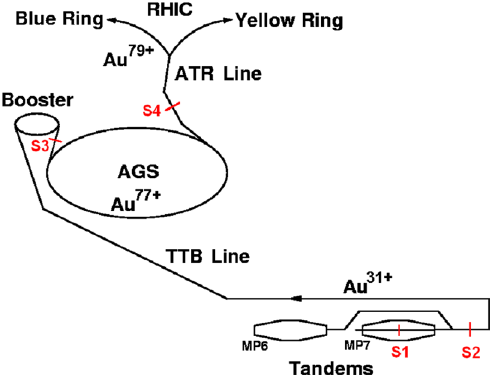
\includegraphics[width=0.45\textwidth]{Figures/Chapter1/AccAu.png}
\caption{The acceleration of gold ions for RHIC is shown above.}
\label{AccAu}
\end{center}
\end{figure} 

At RHIC, we will accelerate the $Au^{79+}$ ions in the superconducting Radio Frequency (RF) cavity under perpendicular electric and magnetic fields until they reach the energies up to about 100 GeV/c per nucleon. Subsequently, we collider them via bunch crossing at the interaction points of the experiments to perform relativistic heavy-ion collisions and study high energy nuclear physics. RHIC usually operates in the first six months of a calendar year. At RHIC, the energy can also be lower where the ion beam collides with ions at a lower energy in the laboratory frame. The STAR experiment at RHIC has already finished beam energy scan and is currently taking data in the fixed target program. 

%RHIC Versatile Machine - Energy + species 

\subsection{Large Hadron Collider (LHC)} 

Located at the border between Switzerland and France, LHC is one of the major high energy accelerator facilities in Europe and currently the highest energy collider in the world. It is a circular collider with a circumference of 26.7 kilometers and can provide proton energy up to 14.0 TeV and lead ion energy up to 5.02 TeV \cite{LHCReport}. It was built in 2008 with the main purpose to discover the Higgs Boson, perform precision measurements on SM, and search for Physics beyond SM. Due to its high energy ion capabilities, high energy nuclear physicists also use the existing general purpose detectors designed for high energy particle experiments at the LHC to conduct research on relativistic heavy-ion physics. LHC ion physics runs usually start at the end of the year and lasts for about a month. The photo taken from the sky to picture LHC is shown in Figure \ref{LHC}:

\begin{figure}[hbtp]
\begin{center}
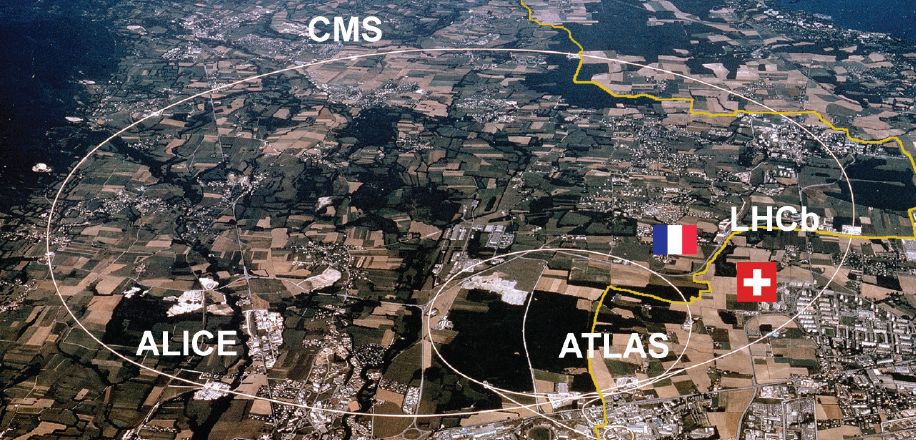
\includegraphics[width=0.85\textwidth]{Figures/Chapter1/LHC.png}
\caption{The sky view of LHC at CERN is shown above. The actual locations of the experiments at the LHC: ATLAS, CMS, ALICE and LHCb, as well as the French-Swiss border, are also displayed.}
\label{LHC}
\end{center}
\end{figure} 

CERN usually uses is lead ${}^{208}_{82} Pb$ ions, which are stable and approximately spherical. In the 2017 ion physics run, it also used the xenon ${}^{131}_{52} Xe$. Currently, there is also a discussion of potential future usage of lighter ions such as oxygen ${}^{32}_{16} O$ \cite{OORun}. Similar to RHIC, the lead ions at the LHC also undergo a series of stripping processes using stripping foils in to order to become partially ionized $Pb^{81+}$ \cite{LHCStrip}. Also, the lead ions pass a series of energy boosting before reaching to the desired energies at the LHC. Lead ions start from a source of vaporized lead and enter Linac 3 before being collected and accelerated in the Low Energy Ion Ring (LEIR) at the energy from 4.2 MeV to 72 MeV. Then, the lead ions will be injected to Proton Synchrotron (PS) to boost their energies. Next, they are sent to the Super Proton Synchrotron (SPS). Finally, the lead ions are injected to the LHC and increase their energies to TeV scale in two LHC rings with the RF cavity \cite{LHCReport}. Finally, the energetic lead ion beams from two LHC rings will collide with a small crossing angle at the interaction points of the LHC experiments. The CERN accelerator complex is shown schematically in \ref{CERNAccComplex} 


\begin{figure}[hbtp]
\begin{center}
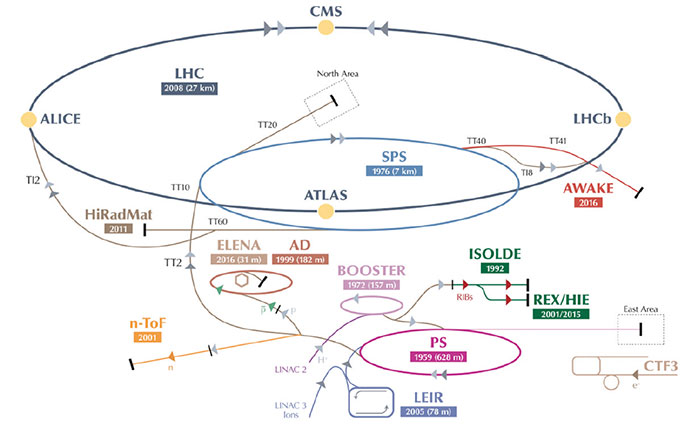
\includegraphics[width=0.65\textwidth]{Figures/Chapter1/CERNAccComplex.jpg}
\caption{The schematic overview of CERN accelerator complex with the accelerators labelled is shown above. Proton and lead ions are accelerated using these facilities and boost their energies to the TeV scale.}
\label{CERNAccComplex}
\end{center}
\end{figure} 

After Run III, LHC will upgrade to high-luminosity (HL) LHC and allows physicists to collect huge datasets, which is crucial to for precision measurements in heavy-ion physics program. Because the beam energy at the LHC is higher than RHIC, the QGP created at the LHC has a higher temperature and a smaller baryon chemical potential than the one created at RHIC.  

\subsection{High Energy Physics Coordinates}

As mentioned in the previous section, heavy-ion is in general highly relativistic. Therefore, Lorentz transformation will be relevant in our studies. In Cartesian coordinates $x^\mu = (t,x,y,z)$, under Lorentz transformation, if we boost the system by a speed $\beta$ in the $+z$ direction. The Lorentz gamma factor will be given by $\gamma = \frac{1}{\sqrt{1 - \beta^2}}$. The four vector $x^\mu \rightarrow x'^\mu$ transforms as follows

\begin{align}
   \begin{bmatrix} 
           t' \\
           x' \\
           y' \\
           z' \\
         \end{bmatrix} =
             \begin{bmatrix} 
             \gamma  & 0  & 0 & - \gamma \beta \\ 
            0 & 1 & 0 & 0 \\ 
             0 & 0 & 1 & 0 \\
             - \gamma  \beta & 0 & 0 &  \gamma \\
	\end{bmatrix} 
	  \begin{bmatrix} 
           t \\
           x \\
           y \\
           z \\
	\end{bmatrix}
\end{align}

The equation above is called the Lorentz Transformation. It is an orthogonal transformation preserving the Minkowski metric tensor $diag(1,-1,-1,-1)$ using particle physicists conventions.


Nowadays, heavy-ion detectors usually have $2\pi$ angular coverage in the transverse direction with some finite longitudinal acceptance along the beam line. They are essentially cylindrically symmetric. Hence, it is convenient and sensible to choose a cylindrical coordinate system and use Lorentz invariant kinematic variables. In general, we define the beam direction to be the z-direction of the coordinate system. Fort the standard cylindrical coordinates in the position space, the Lorentz four-vectors is $(t,x,y,z) \rightarrow (t, r, \phi, z)$. 


The relativistic coordinate system for our analysis is shown below in Figure \ref{HICoordinates}. 

\begin{figure}[hbtp]
\begin{center}
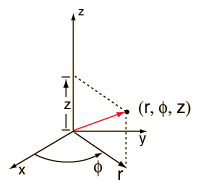
\includegraphics[width=0.40\textwidth]{Figures/Chapter1/PosCylindrical.png}
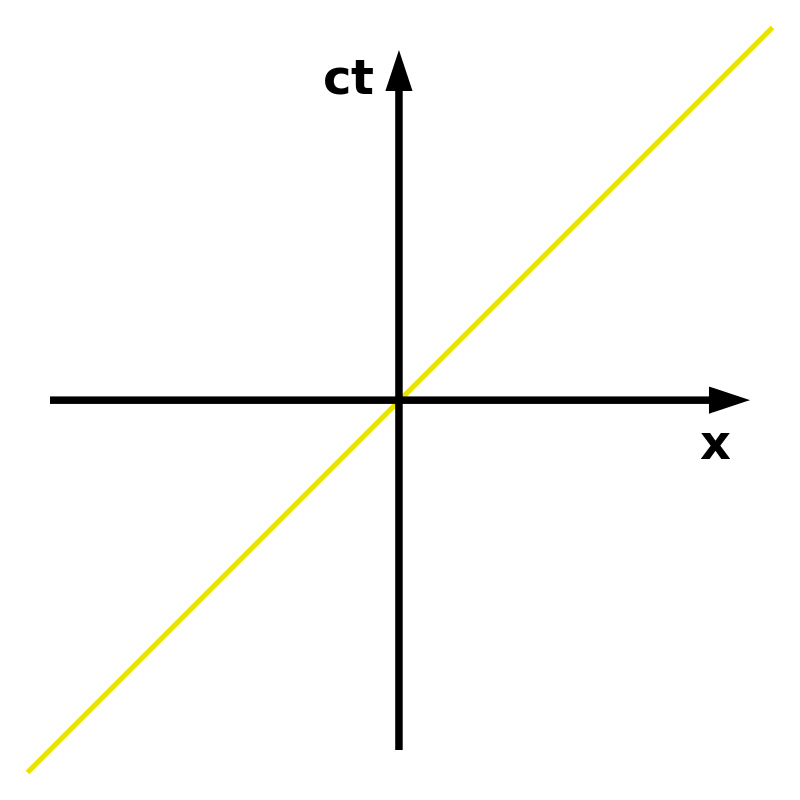
\includegraphics[width=0.40\textwidth]{Figures/Chapter1/STDiagram.png}
\caption{The cylindrical coordinate system in the position space (left) and the space time diagram (right) for relativistic heavy-ion physics analysis are shown above.}
\label{HICoordinates}
\end{center}
\end{figure} 


Thus, in the momentum space, we can use $p^\mu = (E,p_x, p_y, p_z) \rightarrow  (E,p_T, \phi, p_z)$ 

\begin{equation}
p_T = \sqrt{p_x^2 + p_y^2}
\end{equation}

\begin{equation}
\phi = \arctan(\frac{p_y}{p_x})
\end{equation}

We also define rapidity $y$, a relativistic version of velocity that can be convenient add to the boost.

\begin{equation}
y = \frac{1}{2} \ln \frac{E+p_z}{E-p_z}
\end{equation}


Experimentally, we also use pseudo-rapidity $\eta$, which is more directly connected to the detector measurements assuming ultra-relativistic limit kinematics ($E \rightarrow p$). The definition of pseudo-rapidity $\eta$ is shown as follows:

\begin{equation}
\eta =  - \ln \tan(\frac{\theta}{2})
\end{equation}

Here $\theta$ is the angle labelled in the left of Figure \ref{HICoordinates}. Particularly, $y = 0$ and $\eta = 0$ when $p_z = 0$. In addition, boosting by a speed $\beta$ in the longitudinal z-direction, we found that the rapidity simply shift by a const number $y' = y + \tanh \beta$. We should note that the cylindrical coordinates ($p_T$,$\phi$, $p_z$) are perfectly orthogonal while ($p_T$,$\phi$, $y$) or ($p_T$,$\phi$, $\eta$) are not.

For general collider experiments, two particles are moving toward each other with four-momenta $p_1^\mu$ and $p_2^\mu$ and interact with each other. It is also very convenient to use the Mandelstam variables $s, t, u$ in our studies. They are defined as follows

\begin{equation}
s \equiv (p_1 + p_2)^2
\end{equation}

\begin{equation}
t \equiv (p_1 - p_2)^2
\end{equation}

\begin{equation}
u \equiv (p_1 - p_3)^2
\end{equation}


In the center of mass frame, the momentum three vector follows $\vec{p_1} = -\vec{p_2} = \vec{p}$. Therefore, $p_1^\mu = (E, \vec{p})$ and $p_2^\mu = (E, -\vec{p})$. Hence, $s \equiv (p_1 + p_2)^2$ = $4E^2$ = $E_{CM}^2$. Hence, the center of mass energy of the collision system could be represented by the Mandelstam variable $\sqrt{s}$: $E_{CM} = \sqrt{s}$.


%\subsection{Heavy-ion Physics Detectors}

\subsection{Stages of Heavy-Ion Collisions}

In high energy heavy-ion collisions, both Electroweak and QCD processes occur in each event and contribute to the total cross section. We classify the events with elastic and inelastic reaction processes. For elastic processes, two nuclei scatter mainly electromagnetically with each via photon exchange without breaking themselves up or losing energy. For inelastic scattering, we classify diffractive and non-diffractive disassociation processes. In diffractive dissociation processes, the two nuclei may be slightly excited and lose a relatively small fraction of their energies, and produce relatively small number of particles. On the other hand, in non-diffractive dissociation processes, the nuclei lose a substantial fraction of their energies and produce a large number of particles \cite{CYWong}. 

Therefore, in events with significant contribution from non-diffractive dissociation, the interaction between two nuclei has multiple stages including both perturbative and non-pertubative QCD processes. We can define stages of heavy collisions and study the details of each stage. There are five stages: initial state of two highly Lorentz contracted nuclei before the collision, the very early pre-equilibrium stage when hard scatterings between partons inside nuclei begin, the rapid expansion of the fireball when the thermally and chemically equilibrated QGP is created, the hadronization stage after QGP expands and cools down, and the freeze-out stage when the inelastic scattering processes cease.


\begin{figure}[hbtp]
\begin{center}
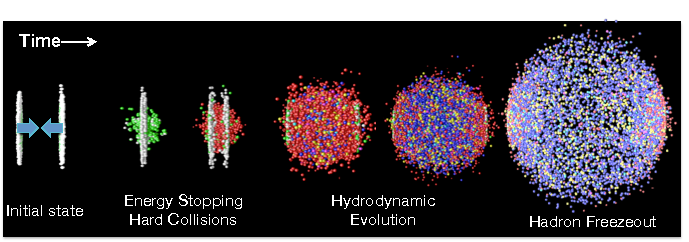
\includegraphics[width=0.80\textwidth]{Figures/Chapter1/Heavy-Ion-Process.png}
\caption{An event of a typical heavy-ion collisions event with different stages as time evolves is shown above.}
\label{HeavyIonStages}
\end{center}
\end{figure} 

\begin{figure}[hbtp]
\begin{center}
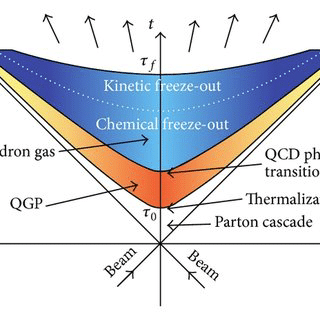
\includegraphics[width=0.45\textwidth]{Figures/Chapter1/HICSTEvolve.png}
\caption{The space-time evolution of heavy-ion collisions is shown above. It consists of four stages: initial state before the collision, early stage of hard scattering processes, the hydrodynamic expansion of QGP, hadronization after QGP expands and cools down, and the freeze-out stage, first chemical freezeout when the particle species no longer change, and finally kinetic freezeout when the elastic scattering processes ceas.}
\label{HICEvolution}
\end{center}
\end{figure} 

Theoretically, many phenomenological models such as Ultra-Relativistic Quantum Molecular Dynamics (UrQMD) and A Multi-Phase Transport Model (AMPT) are developed to describe relativistic heavy-ion collisions. 


\subsection{Global Event Observables}

Globally, we can define some physical quantities in heavy-ion collisions to generally characterize each event. Heavy-ion physicists define the impact parameter, centrality, number of participants, number of binary nucleon-nucleon collisions, and event multiplicity. We will discuss all of them below.

\textbf{Impact Parameter:} Prior to heavy-ion collisions, similar to other collider experiments, each event are prepared with the same unpolarized incoming particles with the same center of mass energy. Therefore, the incoming state $\ket{i}$ is used for each event. However, different from $e^+ e^-$ and $pp$ collision, in heavy-ion physics, we introduce another parameter called the impact parameter denoted $b$ to the transverse distance between center of two nuclei to classify the events. Therefore, the incoming state can be rewritten as  $\ket{i (b)}$. Figure \ref{IPHIColl} shows the definition of impact parameter in heavy-ion collision \cite{IPHICText}.

\begin{figure}[hbtp]
\begin{center}
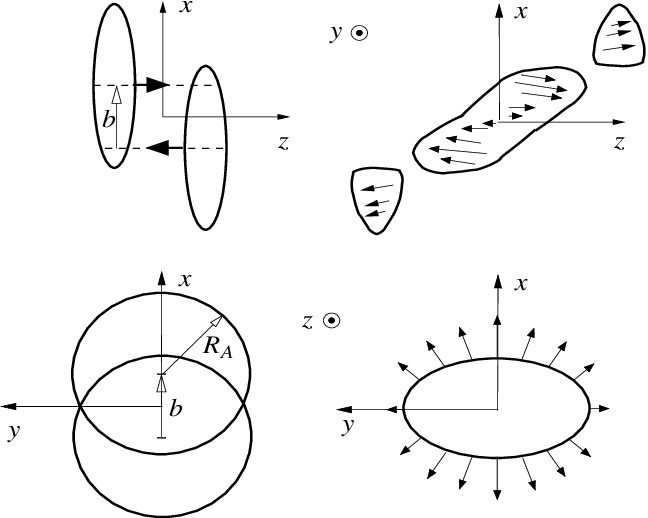
\includegraphics[width=0.60\textwidth]{Figures/Chapter1/IPHIColl.png}
\caption{The definition of impact parameter $b$ in heavy-ion collisions, the of overlapping interaction region, and the break up remnants of the two nuclei, which is called spectator, moving in the z-direction are shown above. An almond shape of the nuclear interaction region, which results in the azimuthal anisotropic emission of final state particles, is seen in heavy-ion collisions.}
\label{IPHIColl}
\end{center}
\end{figure} 


\textbf{Number of Participants:} Right at the end of heavy-ion collisions after two nuclei pass through each other, we can define the number of participants denoted $N_{part}$. The number of participants is essentially equivalent to the number of participating nucleons. The smaller the impact parameter, the more overlap volume between two nuclei, leading to a larger number of number of participating nucleons in the collision. The nuclear interaction system size is determined by the number of participating nucleons. However, due to event-by-event nuclei geometry fluctuations caused by the motion of nucleons inside nuclei \cite{GuntherV3}, it is more proper to say that the average number of participant $\langle N_{part} \rangle$ is related to the impact parameter.

\textbf{Number of Binary Nucleon-Nucleon Collisions:} In addition to $N_{part}$, we can also define another quantity that characterizes the detailed interaction in the events at rather hard scales. The number of binary nucleon-nucleon collisions, denoted $N_{coll}$, is also related to the impact parameter. At higher energy, nucleons inside nuclei become the relevant degree of freedom to describe the cross section. We could treat the collisions of two nuclei as the superposition of the collisions between nucleons inside the nuclei. Since binary nucleon-nucleon collision has a rather small cross section, it dominates the total nucleon-nucleon cross section according to binomial principle. Higher order effects, such as ternary nucleon-nucleon collisions, are negligible. The Glauber model \cite{CentPlot} is developed to study the relationship between $b$, $N_{part}$, and $N_{coll}$ in nuclei collisions and will be discussed in the following subsection.


\textbf{Centrality:} Experimentally, it is difficult to directly measure the impact parameter of each collision. Therefore, we define another physical quantity called centrality to characterize the impact parameter. The centrality ($C$) is defined as the fraction of the total nuclear interaction cross section: $C = \int^b_0 \frac{d\sigma}{dx} dx$ . Centrality is expressed in terms of percentage \cite{CentDef}. It is related to the quantity: $\frac{\pi b^2}{4\pi R_A^2}$ where $R_A$ is the radius of a nuclei defined above in Figure \ref{IPHIColl}. When the impact parameter between two nuclei is 0, the centrality is at 0\%. When the impact parameter between two nuclei is 2$R_A$, the centrality is 100\%. There is also a relationship between the centrality and the average number of participants. Heavy-ion experimental measurements are in general presented in terms of centrality or average number of participants. Experimentally, we look at the number of tracks and cluster energies of calorimeters at the forward direction, for instance, the forward hardonic calorimeters, to estimate the centrality \cite{ALICEZDC,CMSZDC,ATLASZDC}. 


\textbf{Virtuality:} Similar to deep inelastic scattering, we can also define the virtuality $Q^2$, which is the momentum transfer between the two nucleons in nucleon-nucleon collisions. To generate nucleon-nucleon collision event in Monte Carlo (MC) simulation, we used $\hat p_T$, defined as the transverse momentum of the hard subprocess, which is a quantity related to $Q^2$, developed by the high energy theory group of Lund University.


\textbf{Event Multiplicity:} We can also define the event multiplicity by counting the number of final state charged particles to quantify the activity of the event. Event multiplicity can be denoted as $N_{trk}$, number of tracks in the event, which is approximately proportional to the number of charged particle denoted as $N_{ch}$. Figure \ref{CentDefPlot} shows the correlation between the number of participants, their cross section, and the impact parameter in heavy-ion collisions, defining the centrality classes \cite{CentPlot}.


\begin{figure}[hbtp]
\begin{center}
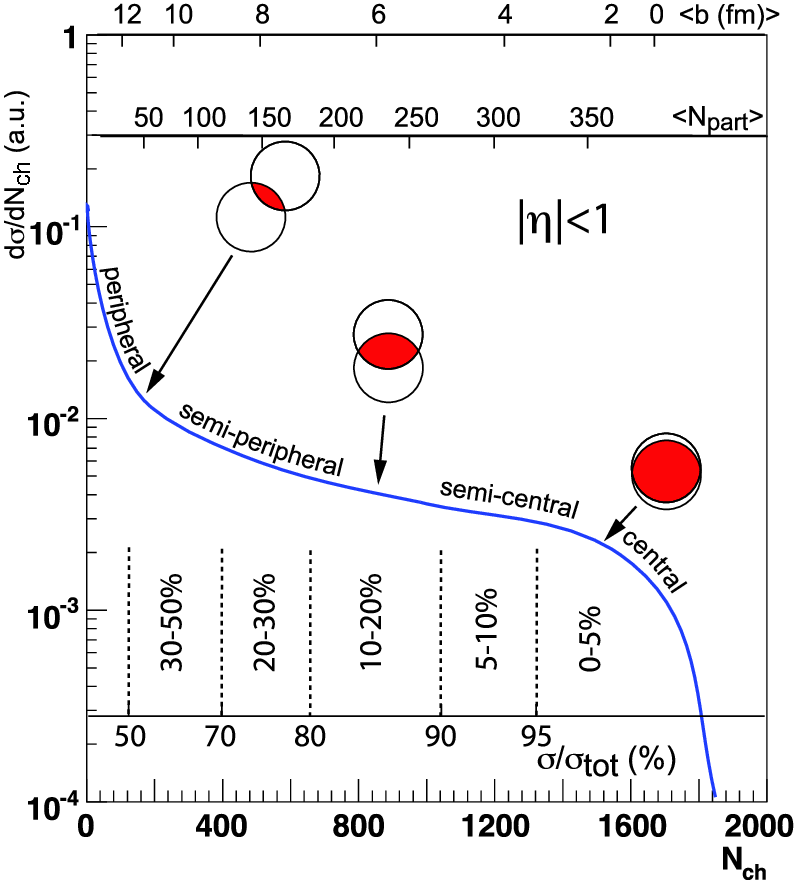
\includegraphics[width=0.55\textwidth]{Figures/Chapter1/CentDefPlot.png}
\caption{The plot showing relationship among number of charged particle, $N_{ch}$, related to the number of participants $N_{part}$, the differential cross section $\frac{d\sigma}{dN_{ch}}$, and the centrality, according to the Glauber Model calculations, is shown above.}
\label{CentDefPlot}
\end{center}
\end{figure} 


The initial global parameters such as the collisions energy, impact parameter, collision nuclei species, and polarization can be treated as knobs for high energy nuclear physicists to play with in order to study relativistic heavy-ion collisions and create strongly interacting systems with different sizes, chemical potentials, and temperatures in the QCD phase diagram. Figure \ref{STAREvtDisplay} shows an event display of thousands of tracks from a central Au + Au collision event at 200 GeV recorded by the Time Projection Chamber (TPC) of the STAR experiment at RHIC.


\begin{figure}[hbtp]
\begin{center}
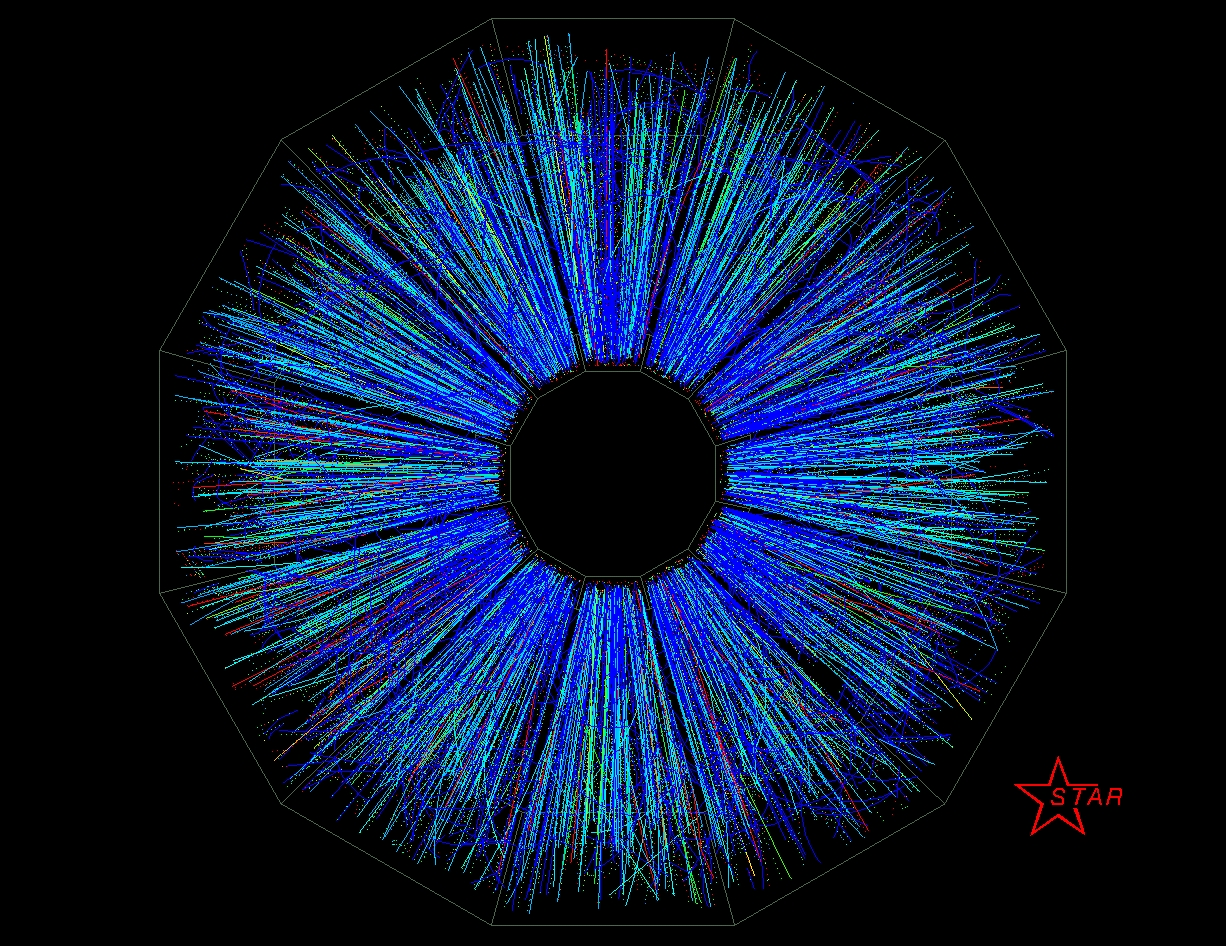
\includegraphics[width=0.50\textwidth]{Figures/Chapter1/STAREvtDisplay.png}
\caption{Two gold ions collide head-on in the STAR detector. The event with reconstructed tracks of final state particles are display by STAR TPC shown above. Image from \cite{STARTPC}}
\label{STAREvtDisplay}
\end{center}
\end{figure} 



\subsection{Glauber Model}

The Glauber Model, named after physicist Roy Glauber \cite{Glauber}, was originally developed to address high energy scattering problems with composite particles in the optical limit where optical theorem is applicable \cite{Optical1,Optical2}. It is a model describing two composite objects collider inelastically with each other and decompose the total cross section to the cross section of collision between two point objects. The Glauber Model can be applied to study nucleon-nucleus (N-A) and nucleus-nucleus (A-B) collisions with nucleon-nucleon (N-N) collisions and determine relationship between the global observables mentioned in the previous subsection.    

If we consider a spherically symmetric nucleus, the nuclear charge density can be described $\rho(r)$ by the Fermi distribution with three parameters below

\begin{equation}
\rho(r) = \rho_0 \frac{1 + w(r/R)^2}{1 + \exp({\frac{r-R}{a}})}
\end{equation}

The equation above is called the Wood-Saxon density formula. According to the Glauber Model \cite{Glauber}, the N-N inelastic cross section is denoted as $\sigma_{in}^{NN}$ and the effective thickness function of a nucleon is defined as a function of impact parameter in the transverse direction: $T(\vec{b})$. It is defined as follow

\begin{equation}
T(\vec{b}) =  \int \rho(\vec{b},z) dz 
\end{equation}

It is normalized to unity: $\int^{R_A}_0 T(\vec{b}) d^2b = 1$. $T(\vec{b})$ essentially depends on density of the nucleus $r(b)$. %If the nucleus is a uniform cylinder and the collide on its circular face along its height, then $T(\vec{b})$ will be a constant. 
Therefore, the probability that a nucleon collides with a nucleon inside the nucleus is given by $\sigma_{in} T(\vec{b})$. Therefore, the probability of $n$ nucleon collisions is given by

\begin{equation}
P_n = {A \choose n} \sigma_{in}^{NN} T(\vec{b})^{n} [1 - \sigma_{in} T(\vec{b})]^{A-n}
\end{equation}

Hence, if we consider a constant fraction of $\mu$ ($0 \le \mu \le 1$) of particle produced after each collisions, we can calculation the average event multiplicity $\langle N(\mu) \rangle$:

\begin{equation}
\langle N(\mu) \rangle = \Sigma_n P_n \Sigma^{n-1}_0 \mu^m =  \Sigma_{n-1} P_n \frac{1 - \mu^n}{1 - \mu} = \frac{1}{1-\mu} \{ 1 - [1 - (1-\mu) \sigma_{in} T(\vec{b})]^A \}
\end{equation}

It turns out that we have the following relationship between $N_{part}$ and $N_{coll}$ with $\langle  N(\mu) \rangle$  \cite{Glauber}

\begin{equation}
N_{part} = \langle N(\mu = 0) \rangle 
\end{equation}

\begin{equation}
N_{coll} = \frac{1}{2} \langle N(\mu = 1) \rangle = A T(\vec{b}) \sigma_{in}^{NN}
\end{equation}

In a more generalized case: A-B collisions, Figure \ref{GlauberRef} shows side view and beam-line view of heavy-ion collision of projectile B on target A


\begin{figure}[hbtp]
\begin{center}
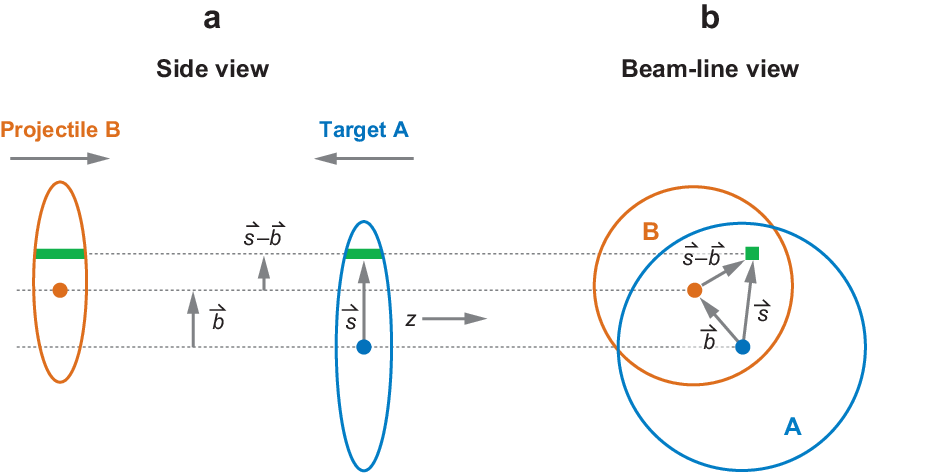
\includegraphics[width=0.65\textwidth]{Figures/Chapter1/GlauDefColl.png}
\caption{The A-B collision with the definition of the impact parameter vector $\vec{b}$ and the distance of nucleon to the center of projectile B $\vec{s}$ are shown above. The distance of the nucleon in B to center of the target A is $\vec{s}-\vec{b}$ according to vector subtraction rule. Here we assume both nuclei A and B are perfect spheres.}
\label{GlauberRef}
\end{center}
\end{figure} 

Using similar ideas \cite{CentPlot}, we could first calculate the effective thickness function $T_{AB}$ as follows:


\begin{equation}
T_{AB}(\vec{b}) = \int T_A(\vec{s}) T_B(\vec{b} - \vec{s}) d^2s 
\end{equation}



Now replacing T($\vec{b}$) in N-A by $T_{AB}(\vec{b})$ in A-B, we can obtain

\begin{equation}
\langle N(\mu) \rangle = \frac{A}{1-\mu} \int_0^b T_A(\vec{s}) \{1 - [1 - (1 - \mu) T_{B}(\vec{b}-\vec{s}) \sigma_{in}^{NN}]\}^A d^2s  +  \frac{B}{1-\mu} \int_0^b T_B(\vec{s}) \{1 - [1 - (1 - \mu) T_{A}(\vec{b}-\vec{s}) \sigma_{in}^{NN}]\}^B d^2s
\end{equation}


To obtain $N_{part}$, evaluate at $\mu = 0$, we get 

\begin{equation}
N_{part} =  A \int_0^b T_A(\vec{s}) \{1 - [1 - T_{B}(\vec{b}-\vec{s}) \sigma_{in}^{NN}]^A\}d^2s +  B \int_0^b T_B(\vec{s}) \{1 - [1 - T_{A}(\vec{b}-\vec{s}) \sigma_{in}^{NN}]^B\} d^2s
\end{equation}

To obtain $N_{coll}$, evaluate at $\mu = 1$, we get

\begin{equation}
N_{coll} = AB T_{AB}(\vec{b}) \sigma_{in}^{NN}
\end{equation}

In a very special case, assume the nuclei are simply perfect rigid sphere with the same radius and collide with zero impact parameter is $b=0$. That is $T_{A} \sigma_{in}^{NN} = T_{B} \sigma_{in}^{NN} = T_{AB} \sigma_{in}^{NN} = 1$, we get 


\begin{equation}
N_{part} = A + B
\end{equation}

\begin{equation}
N_{coll} = AB
\end{equation}

The results above of $N_{part}$ and $N_{coll}$ agree to our expectation. 

The comparison of the Glauber Model with simulations of the $N_{part}$ and $N_{coll}$ as a function of impact parameter $b$ is shown on Figure \ref{NPartandNColl} from the \cite{CentPlot}

\begin{figure}[hbtp]
\begin{center}
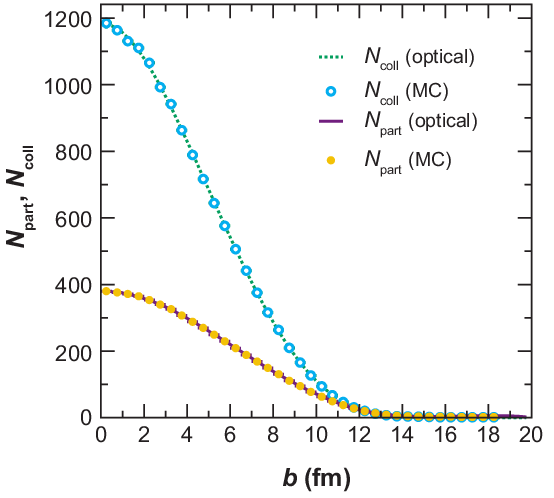
\includegraphics[width=0.50\textwidth]{Figures/Chapter1/NPartandNColl.png}
\caption{The $N_{part}$ and $N_{coll}$ as a function impact parameter calculated from the Glauber Model with optical approximation (lines) and from MC simulations (circles) are shown above. We can see they have almost perfect agreement with each other.}
\label{NPartandNColl}
\end{center}
\end{figure} 


Therefore, we can apply the Glauber model to determine $N_{part}$ and $N_{coll}$ for a given centrality range of AA collision ($T_{AB} \rightarrow T_{AA}$), which will be used in our analysis to obtain the corrected yield. It has been reported that the production of light hadrons, such as pions and kaons, are scaled as $N_{part}$ \cite{NPartScaling} while electroweak bosons, such as W and Z boson, are scaled as $N_{coll}$ \cite{NCollScaling}.

\section{Characterization of Quark-Gluon Plasma}

Equipped with the knowledge and collider technologies of heavy-ion collisions, we are ready to apply them to conduct scientific research on QGP in laboratories. The following subsections will describe the characterization of QGP from its predicted signatures to open questions today, which leads to my thesis research.

\subsection{Signatures}

QGP has been hypothesize long before its discovery as a color deconfined phase of quark matter named ``quark gluon plasma'' \cite{LeonQGP} and will demonstrate some specific benchmarks in experiments to prove the creation of QGP \cite{QGPSignature}. Here, four classic signatures of QGP will be discussed: $J/\psi$ and $\Upsilon$ suppression, jet quenching, elliptic flow, strangeness enhancement.  

\subsection{$J/\psi$ and $\Upsilon$ suppression} 

$J/\psi$ meson, as a type of heavy quarkonia, is bound state of $c\bar c$, made of charm quark and an anti-charm quark, with mass heavier than the $\Lambda_{QCD}$. Therefore, we could approximately treat the interaction between charm and the anti-charm quark with a static the Cornell potential $V(r)$ in the non-relativistic quantum mechanical hamiltonian system \cite{QuarkoniaV}: 

\begin{equation}
\hat H = \hat T + \hat V
\end{equation}

\begin{equation}
\hat H \ket{\psi} = i \frac{\partial}{\partial t}  \ket{\psi} 
\end{equation}

and solve Schrodinger equation the to describe $J/\psi$ mesons in vacuum. As we have seen in Section 1.3.2, with the QGP medium, at a finite temperature $T$, the potential is modified due to color screening effect. The distance between two charm quarks $V(r) \rightarrow \frac{\sigma}{m_D}$, which does not diverge, as $r \rightarrow \infty$. Therefore, the $c \bar c$ system could be unbounded if they have sufficiently high energy. In the field theory picture, this could be understood as the color string breaking between charm and anti-charm quark \cite{CSBQQ}, also known as quarkonia melting \cite{QQMelt}. Hence, with the influence of QGP at $T > 0$, the production cross section of $J/\psi$ will decrease compared to the vacuum at $T=0$. Experimentally, we define an observable to quantify the modification of particle production cross section in $AA$ collision compared to the reference $pp$ collisions normalized by the number of binary nucleon-nucleon collisions $N_{coll}$, which is defined in the previous subsection. We called this observable as nuclear modification factor denoted $R_{AA}$. Mathematically, $R_{AA}$ is defined as follows:

\begin{equation}
R_{AA} =\frac{1}{N_{coll}} \frac{\frac{d^2N_{AA}}{dp_T dy}}{\frac{d^2N_{pp}}{dp_T dy}} = \frac{1}{T_{AA}} \frac{\frac{d^2N_{AA}}{dp_T dy}}{\frac{d^2\sigma_{pp}}{dp_T dy}}
\end{equation}

Therefore, $R_{AA} < 1$ means suppression. $R_{AA} =1$ means no modification. $R_{AA} > 1$ means enhancement. Hence, in experiments, we expect to observe the $R_{AA} < 1$ a suppression of $J/\psi$ production. Figure \ref{JPsiSupp} shows the measurement of fully reconstructed $J/\psi$ at RHIC and LHC \cite{STARJpsi}


\begin{figure}[hbtp]
\begin{center}
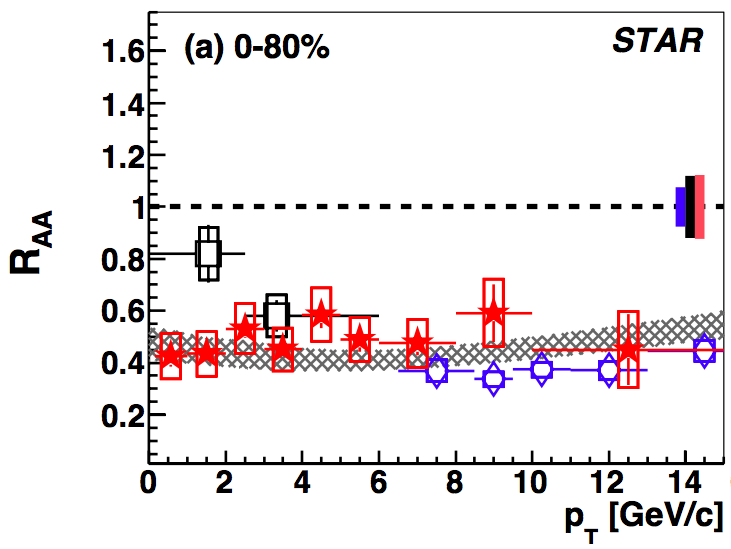
\includegraphics[width=0.47\textwidth]{Figures/Chapter1/STARPt.png}
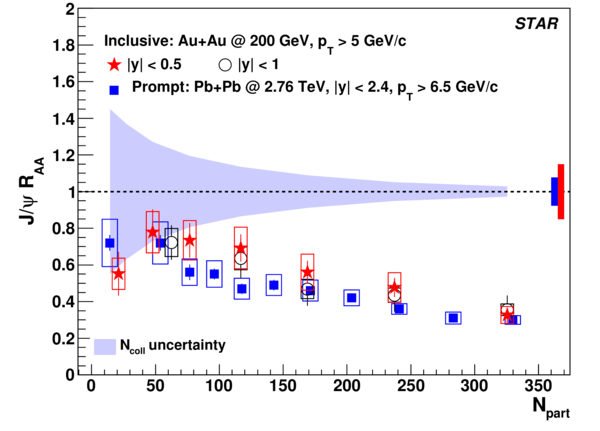
\includegraphics[width=0.487\textwidth]{Figures/Chapter1/STARNPart.png}
\caption{The nuclear modifications factor $R_{AA}$ of fully reconstructed $J/\psi$ as a function of $p_{T}$ (left) and $N_{part}$ (right) measured by the STAR experiment (red data points) at RHIC and CMS (blue diamond data points) and the ALICE (blue circle data points) experiment at the LHC are shown above. We can see that the $J/\psi$ $R_{AA}$ is below 1 for both $p_T$ and $N_{part}$. There is no significant $p_T$ dependence of $J/\psi$ $R_{AA}$. The $J/\psi$ $R_{AA}$ decreases as $N_{part}$ increases, consistent to the increasing creation probability of QGP with larger $N_{part}$.}
\label{JPsiSupp}
\end{center}
\end{figure} 

In fact, we could see that $R_{AA} < 1$ for every data point, which indicates a clear suppression of $J/\psi$ production from experiments at both RHIC and the LHC. However, we should note that the larger $J/\psi$ $R_{AA}$ observed at the LHC compared to RHIC could be explained by regeneration mechanism \cite{JPsiRegen}. %The observation of $J/\psi$ suppression is one of the earliest evidence of the discovery of QGP.

Similarly, we expect to see this in $\Upsilon$, which is made of $b \bar b$. Indeed, they expect to have sequential suppression since 3 $\Upsilon$ states: $\Upsilon(1S)$,  $\Upsilon(2S)$, and $\Upsilon(3S)$, could be observed in experiments. Because the total energy of the $b \bar b$ system or equivalently the rest mass: $m_{\Upsilon(3S)} > m_{\Upsilon(2S)} > m_{\Upsilon(3S)}$, a sequential suppression: $R_{AA}^{\Upsilon(1S)} > R_{AA}^{\Upsilon(2S)} > R_{AA}^{\Upsilon(3S)}$ should be observed if QGP is created. Figure \ref{UpsilonSupp} shows the measurements of fully reconstructed $\Upsilon$ states at RHIC and LHC \cite{STARUpsilonRef,CMSUpsilonRef}

\begin{figure}[hbtp]
\begin{center}
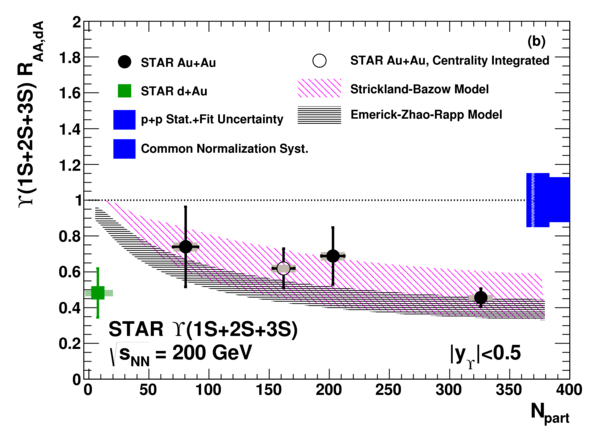
\includegraphics[width=0.52\textwidth]{Figures/Chapter1/STARUpsilon.png}
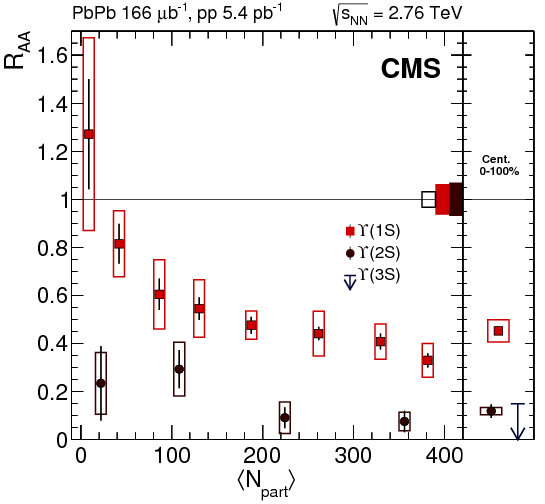
\includegraphics[width=0.40\textwidth]{Figures/Chapter1/CMSUpsilon.png}
\caption{The nuclear modifications factor $R_{AA}$ of fully reconstructed $\Upsilon$ as a function of $N_{part}$ measured by the STAR experiment (left) at RHIC and CMS experiment (right) at the LHC are shown above. We can see that the $R_{AA}$ of the three $\Upsilon$ states are below 1 when $N_{part} > 3$. The $\Upsilon$ $R_{AA}$ decreases as $N_{part}$ increases, consistent to the increasing creation probability of QGP with larger $N_{part}$. In addition, a sequential suppression of $\Upsilon$ $R_{AA}$ is observed by the CMS experiment: $R_{AA}^{\Upsilon(1S)} > R_{AA}^{\Upsilon(2S)} > R_{AA}^{\Upsilon(3S)}$, which agrees with the expectation QGP color screening effect.}
\label{UpsilonSupp}
\end{center}
\end{figure} 


\subsection{Jet Quenching} 

Experimentally, due to color confinement, it is impossible to directly detect and track the energetic partons. Therefore, physicists define jet as a spray of collimated hadrons within a narrow cone initiated from color charged partons. In nuclear and particle physics, jets are used to study the dynamics of partons before hadronization \cite{HERAJET} and understand the properties of QGP. A schematic view of a di-jet production from di-qurark event in electron-positron collider $e^+e^-\rightarrow q \bar q$ is shown below in Figure \ref{dijet}


\begin{figure}[hbtp]
\begin{center}
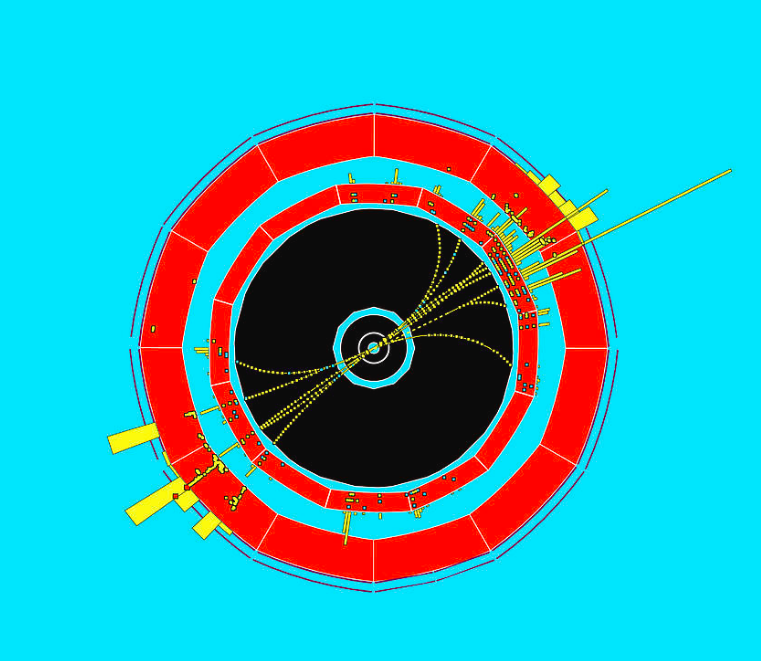
\includegraphics[width=0.50\textwidth]{Figures/Chapter1/DijetEvt.png}
\caption{The schematic display of a di-jet event from the ALEPH (a particle detector at the Large Electron-Positron collider) Experiment at the Large Electron-Positron Collider (LEP) is shown above. We can see two sprays of back to back particles within narrow cone, representing a di-jet event.}
\label{dijet}
\end{center}
\end{figure} 


Since we know QGP a color deconfined state of matter, an energetic parton carrying color charge traveling through the QGP medium is expected to lose a substantial a mount its energy to the medium. This is similar the effect that an electron beam losing energy in the electron-ion plasma via electromagnetic interaction \cite{ELossPlasma}. We call this effect as jet quenching. Figure \ref{JetELoss} shows jet quenching in QGP in AA collisions compared to pp collisions

\begin{figure}[hbtp]
\begin{center}
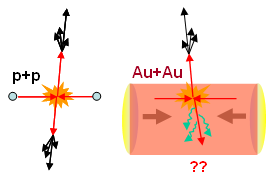
\includegraphics[width=0.45\textwidth]{Figures/Chapter1/JetELoss.png}
\caption{The schematic picture explaining jet quenching is shown above. Hard scatterings in pp collisions produce back-to-back "jets" of particles, but in Au + Au collisions, the presence QGP modifies the jets' properties.}
\label{JetELoss}
\end{center}
\end{figure} 


Experimentally, compared to pp collision where the QGP is not expected to be created, the jet spectra is modified by the QGP medium. The angular distributions would be broaden due to interaction with the medium. The $p_T$ spectra will be shifted to the left due to energy loss. This can be quantified by jet nuclear modification factor $R_{AA}$ similar to the $R_AA$ for quarkonium suppression mentioned previously. Figure \ref{JetRAA} shows the hadron angular correlation with the STAR experiment at RHIC and jet $R_{AA}$ as a function of $p_T$ with the ALICE experiments at LHC \cite{STARJetRef,ALICEJetRef}:
  
\begin{figure}[hbtp]
\begin{center}
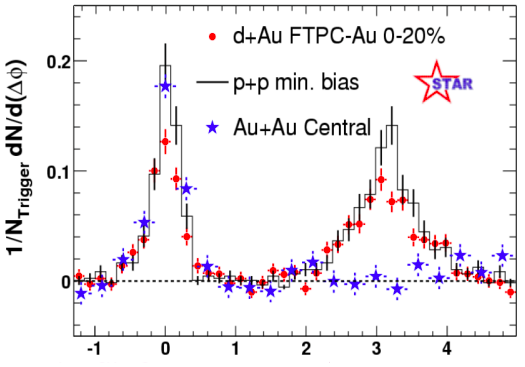
\includegraphics[width=0.55\textwidth]{Figures/Chapter1/HadronAngularSTAR.png}
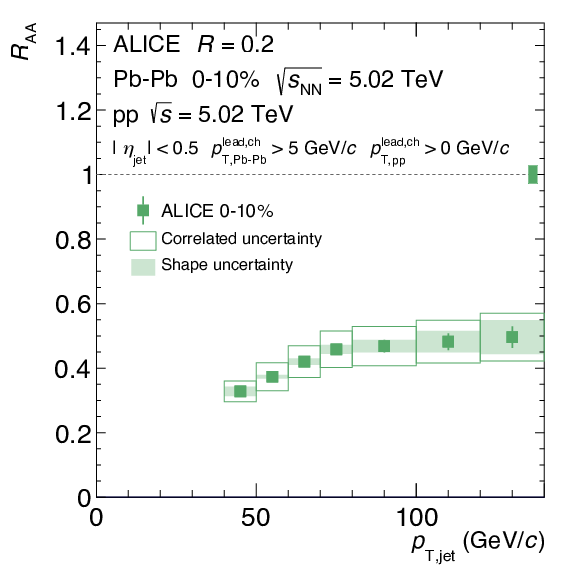
\includegraphics[width=0.40\textwidth]{Figures/Chapter1/JetRAAALICE.png}
\caption{The comparison of two-particle azimuthal distributions for central d + Au collisions to those seen in $pp$ and central Au + Au collisions measured with the STAR experiment and the jet $R_{AA}$ as a function $p_T$ measured by the ALICE experiment at LHC (right). From the STAR result, in central Au + Au collisions, the back-to-back peak has disappeared due to the redistribution of jet energy to the slow expanding medium constituents. The jet $R_{AA}$ from ALICE measurement is clearly below 1, suggesting that jets lose significant fractions of energy in $AA$ collision compared to $pp$.}
\label{JetRAA}
\end{center}
\end{figure} 

The jet $R_{AA}$ are all below 1 at RHIC and LHC \cite{ALICEJetRef,CMSJetSub}, which suggest jet quenching in AA collisions, supporting existence of QGP.

\subsection{Elliptic Flow} 

The reaction region in heavy-ion collisions, where the two nuclei overlap with each other, has an almond shape, which is azimuthally asymmetric. If a color deconfined matter QGP is created, particles emitted from the almond shape fire ball are expected to be anisotropic due to differences of the pressure gradient of the QGP in the and their path length through QGP in the x and y direction. Experimentally, physicists Dr. Arthur Poskanzer who sadly just passed away in June 30 2021, and Dr. Sergey Voloshin developed the event plane method to analyze the azimuthal anisotropy of particle emission in heavy-ion collisions \cite{EllipticFlow}. The reaction plane is defined as the plane of the impact parameter and the x-axis. Figure \ref{EventPlane} schematically shows the definition of reaction plane in heavy-ion collisions.

\begin{figure}[hbtp]
\begin{center}
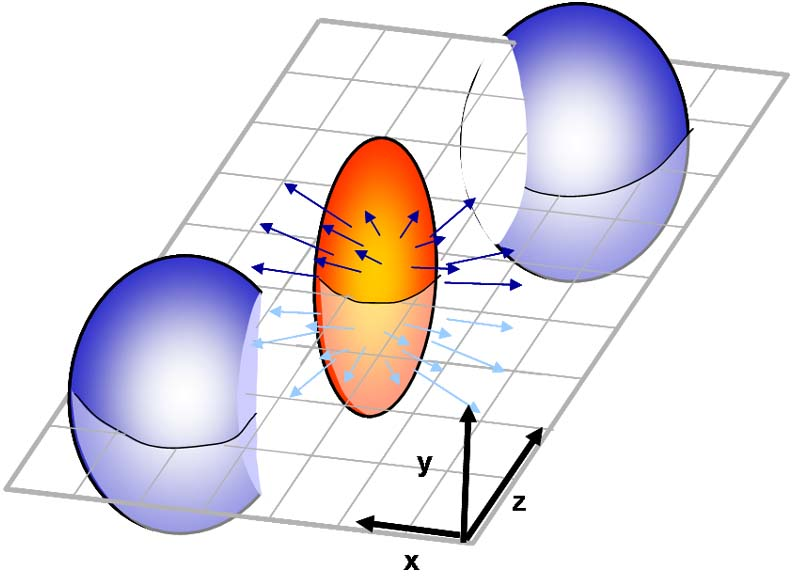
\includegraphics[width=0.40\textwidth]{Figures/Chapter1/ReactionPlane.jpg}
\caption{The figure above shows the ellipsoid of the overlapping nuclear reaction region of two nuclei in heavy-ion collisions. The reaction plane, which is the x-z plane shown as above, is constructed by the beam direction and the impact parameter vector. The emissions of particles are azimuthally anisotropic in the x-y plane.}
\label{EventPlane}
\end{center}
\end{figure} 

The particle spectra in heavy-ion collisions can be factorized as 

\begin{equation}
E \frac{d^3N}{d^3p} = E \frac{1}{2 \pi p_T}\frac{d^3N}{dp_T dy d\phi} = E \frac{1}{2 \pi p_T} \frac{d^2N_1}{dp_T dy} \frac{dN_2}{d\phi}
\end{equation}

Since the particle emission is azimuthally anisotropic, we can expand the $F(p_T,\phi,y) = \frac{dN_2}{d\phi}$ into a Fourier series \cite{EllipticFlow}:


\begin{equation}
F(p_T,\phi,y) = \frac{x_0(p_T,y)}{2\pi}  + \sum_{n=1}^{\infty}[x_n(p_T,y)\cos(n\phi)+y_n(p_T,y)\sin(n\phi)] 
\end{equation}

According to trigonometry, we get

\begin{equation}
F(p_T,\phi,y)  = \frac{x_0(p_T,y)}{2\pi} + \sum_{n=1}^{\infty}2v_n(p_T,y)\cos[n(\phi - \Psi_{n})]
\end{equation}

Here, $v_n = \frac{1}{2} \sqrt{x_n^2 + y_n^2}$ and $\Psi_{n} =\frac{1}{n} \arctan(\frac{y_n}{x_n})$. 

To find the Fourier coefficients $v_n$, we can apply the Fourier tricks to find $x_n$ and $y_n$.


Theoretically, because the function $\frac{dN_2(\phi)}{d\phi}$ is continuously analytical, we can use integral to find the Fourier coefficients [18] 
\begin{equation}
x_n =2\int_{0}^{2\pi} \frac{dN_2(\phi)}{d\phi}\cos(n\phi)d\phi 
\end{equation}
\begin{equation}
y_n =2\int_{0}^{2\pi} \frac{dN_2(\phi)}{d\phi}\sin(n\phi)d\phi 
\end{equation}

Experimentally, because our data take on discrete values, we can convert the integral into a sum 
\begin{equation}
x_n =\frac{2}{N}\sum_{n=1}^{N} \cos(n\phi)d\phi = 2\langle \cos n\phi \rangle
\end{equation}
\begin{equation}
y_n =\frac{2}{N}\sum_{n=1}^{N} \sin(n\phi)d\phi = 2\langle \sin n\phi \rangle
\end{equation}

Here, we sum up all tracks in the experiment to get the $x_n$ and $y_n$. Then, we will be able to find 

\begin{equation}
v_n = \frac{1}{2} \sqrt{x_n^2 + y_n^2} = \sqrt{(\langle \cos n\phi \rangle)^2+(\langle \sin n\phi \rangle)^2}. 
\end{equation}




In heavy-ion physics, the first order Fourier coefficient $v_1$ is called the directed flow. 

\begin{equation}
v_1 =  \sqrt{(\langle \cos \phi \rangle)^2+(\langle \sin \phi \rangle)^2}. 
\end{equation}

It can be connected to the initial tilting source of the colliding nuclei \cite{V1Tilted} and can be used to study Chiral Magnetic Effect \cite{V1CME}. 

The second order Fourier coefficient $v_2$ is called elliptic flow. 

\begin{equation}
v_2 =  \sqrt{(\langle \cos 2\phi \rangle)^2+(\langle \sin 2\phi \rangle)^2} =  \sqrt{(\langle \cos^2 \phi \rangle - \langle \sin^2 \phi \rangle)^2 + (2  \langle \sin \phi \rangle \langle \cos \phi \rangle)^2}. 
\end{equation}

Assuming in initial stage before the collision, the sum of the momentum of two colliding nuclei $\vec p_1$ and $\vec p_2$ is exactly 0 without any fluctuation. That is

\begin{equation}
\vec{p_1} + \vec{p_2} = 0
\end{equation}

According to momentum conservation, for the final state particles, we have 

\begin{equation}
\sum_i^N p_x^i = 0
\end{equation}

\begin{equation}
\sum_i^N p_y^i = 0
\end{equation}

Therefore, we have

\begin{equation}
\langle p_T \cos \phi \rangle = \langle p_x \rangle = \frac{1}{N} \sum_i^N p_x^i   = 0
\end{equation}

\begin{equation}
\langle p_T \sin \phi \rangle = \langle p_y \rangle =  \frac{1}{N} \sum_i^N p_y^i  = 0
\end{equation}
 
But since the $p_T$ and $\phi$ are completely orthogonal, the random variable $p_T$ is uncorrected to $\phi$. Therefore, we have 
 
\begin{equation}
\langle p_T \cos \phi \rangle =  \langle p_T \rangle \langle  \cos \phi \rangle = 0
\end{equation}

\begin{equation}
\langle p_T \sin \phi \rangle =  \langle p_T \rangle \langle  \sin \phi \rangle = 0
\end{equation}

Finally, we know that $p_T > 0$, thus   
 
\begin{equation}
\langle p_T \rangle > 0
\end{equation}  
 
Hence,  


\begin{equation}
\langle \cos \phi \rangle =  0
\end{equation} 


\begin{equation}
\langle \sin \phi \rangle =  0
\end{equation}

Therefore, we have 

\begin{equation}
v_2 = \sqrt{(\langle \cos^2 \phi \rangle - \langle \sin^2 \phi \rangle)^2 + (2  \langle \sin \phi \rangle \langle \cos \phi \rangle)^2} = \langle \cos^2 \phi \rangle - \langle \sin^2 \phi \rangle. 
\end{equation}

In terms of momentum $p_x$ and $p_y$, we can rewrite $v_2$ as 

\begin{equation}
v_2 =  \langle \cos^2 \phi \rangle - \langle \sin^2 \phi \rangle = \langle\frac{p_x^2}{p_T^2} \rangle - \langle \frac{p_y^2}{p_T^2} \rangle = \langle \frac{p_x^2 - p_y^2}{p_T^2} \rangle = \langle \frac{p_x^2 - p_y^2}{p_x^2 + p_y^2} \rangle. 
\end{equation}

Classically, we know that the momentum is proportional to the pressure gradient. Schematically, we could write

\begin{equation}
p_x \simeq \frac{m\tau}{\rho}\frac{\partial P}{\partial x} \simeq \frac{m\tau}{\rho}\frac{P}{L_x}
\end{equation}

Where $m$ is the mass of the particle, $\tau$ is the life time of the QGP, $\rho$ is the density of the QGP, and $L_x$ is the minor axis of the ellipse in the x direction according to the geometry of Figure \ref{EventPlane}.

Likewise, we have the same relation for $p_y$

\begin{equation}
p_y \simeq \frac{m\tau}{\rho}\frac{\partial P}{\partial y} \simeq \frac{m\tau}{\rho}\frac{ P}{L_y}
\end{equation} 

Here,  $L_y$ is the major axis of the ellipse in the y direction according to the geometry of Figure \ref{EventPlane}. Apparently, $L_y > L_x$. 

Hence, we can write $v_2$ as 
\begin{equation}
v_2 =  \langle \frac{p_x^2 - p_y^2}{p_x^2 + p_y^2} \rangle = \frac{\frac{1}{L_x^2} - \frac{1}{L_y^2}}{\frac{1}{L_x^2} + \frac{1}{L_y^2}} =  \frac{L_y^2 - L_x^2}{L_x^2 + L_y^2}  > 0
\end{equation}

In heavy ion collision, we define the eccentricity $\epsilon_s$ of an ellipse is defined as \cite{V2Eccent}

\begin{equation}
\epsilon_s \equiv \frac{L_y^2 - L_x^2}{L_x^2 + L_y^2}
\end{equation}

Hence, we have

\begin{equation}
v_2 \simeq \epsilon_s
\end{equation}

Therefore, we can see that $v_2$ is essentially proportional to the eccentricity simply based on ellipse geometry of reaction region. Historically, $v_2$ has extensively studied experimentally and theoretically. It turns out light hadrons demonstrate collectivity. Their elliptic flow $v_2$ could be calculated using relativistic viscous hydrodynamics, which we will describe in the next section. If QGP is created, we expect $v_2$ of the light flavor hadrons created direction from the QGP to be positive as we derive above. Figure \ref{V2} show the $v_2$ as a function of $p_T$ of charged light flavor hadrons in heavy-ion collisions at mid-rapidity measured by RHIC and LHC experiment \cite{V2STAR,V2ALICE}

\begin{figure}[hbtp]
\begin{center}
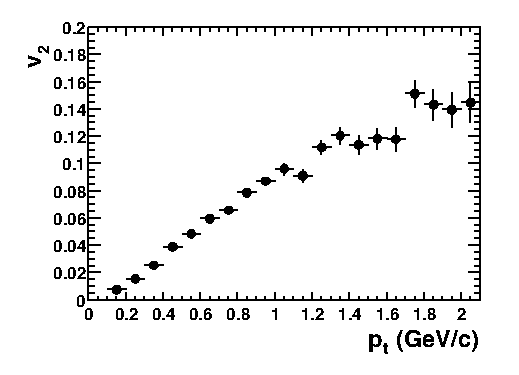
\includegraphics[width=0.45\textwidth]{Figures/Chapter1/STARV2Plot.eps}
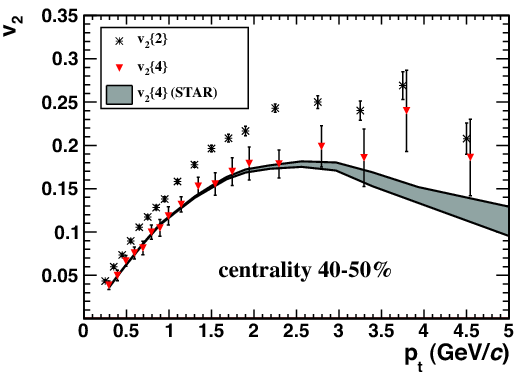
\includegraphics[width=0.45\textwidth]{Figures/Chapter1/ALICEV2Plot.png}
\caption{The elliptic flow of charged particles $v_2$ as a function of $p_T$ in AuAu collision measured by the STAR experiments at RHIC (left) and in PbPb collisions by the ALICE experiments at LHC (right) are shown above. Clearly, $v_2 > 0$ is observed in both experiments.}
\label{V2}
\end{center}
\end{figure}   

We can clearly see positive $v_2$ of charged particles at both RHIC and LHC, which also supports the creation of QGP in high energy heavy-ion collisions.  
 
\subsection{Strangeness Enhancement} 

As described in Section 1.4.6, the temperature of QGP is well above 100 MeV, which is much larger than the strange quark mass (about 95 MeV). Therefore, since $T_{QGP} > m_s$, in thermally and chemically equilibrated QGP, strange quarks could be produced thermally via the pair production process $u \bar u, d \bar d \rightarrow s\bar s$, and $gg \rightarrow s \bar s$, creating the chemical abundance equilibrium \cite{SSEnhance}. Therefore, the strangeness content in the QGP is enhanced, which could be experimentally observed from enhancement of strange particle yields in AA collisions compared to pp collisions. A direct experimental observable is the ratio of strange hadron yield to pions in AA and pp collisions. Figure \ref{PhiRAA1} and \ref{PhiRAA2} shows measurements on strange meson and baryons to pion ratios in AA and pp at RHIC and LHC 

\begin{figure}[hbtp]
\begin{center}
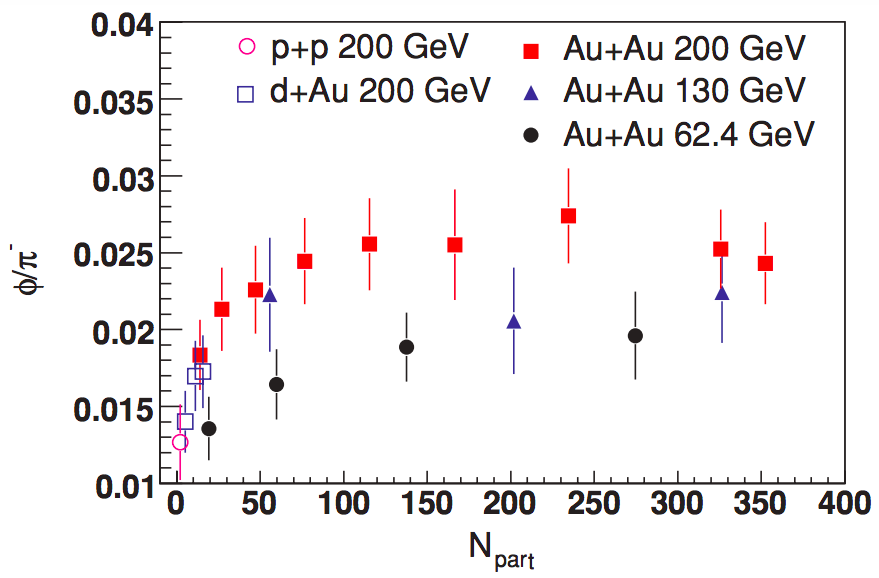
\includegraphics[width=0.45\textwidth]{Figures/Chapter1/STARPhiOverPi.png}
\caption{The yield ratio of $\phi/\pi$ as a function $N_{part}$ in p + p, p + Au, and Au + Au from the STAR experiment at RHIC are shown above.}
\label{PhiRAA1}
\end{center}
\end{figure}   

\begin{figure}[hbtp]
\begin{center}
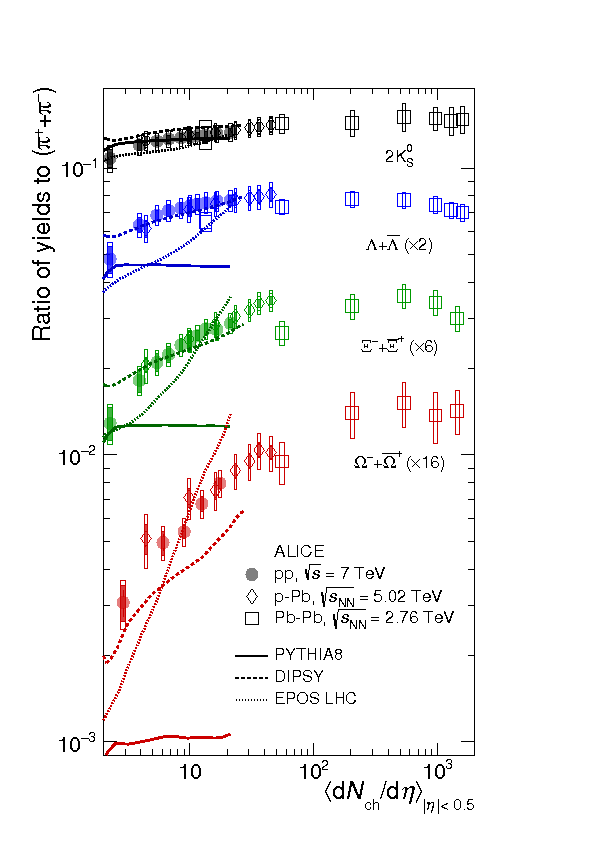
\includegraphics[width=0.60\textwidth]{Figures/Chapter1/ALICEStrange.png}
\caption{The yield ratio of strange hadrons $K^0_s, \Lambda^+, \Xi^0, \Omega^-$ as a function of $\langle dN_{ch}/d\eta \rangle$ from the ALICE experiment at LHC are shown above.}
\label{PhiRAA2}
\end{center}
\end{figure}   

We can see that $\phi/\pi$ ratio increases as $N_{part}$ and $\sqrt {s_{NN}}$ increases, which indicates strangeness enhancement in AA collisions compare to pp collisions. This again can be served as an evidence for the formation of QGP in heavy-ion collisions at RHIC and LHC. 

%J/psi suppression, jet quenching, elliptic flow, strangeness enhancement 

\subsection{Macroscopic Properties}

Physicists have conducted extensive studies to pin down macroscopic properties of QGP. 

\textbf{Transient Lifetime:} According to experimental results at RHIC and LHC, QGP has a very short lifetime. It is on the order of 10 fm/c \cite{QGPLifeTime}. It is generally assumed that QGP reaches thermal \cite{QGPThermal} and near chemical equilibrium \cite{QGPChemical} via the strong interaction. So far, there is not sufficient experimental evidence to directly support this assumption.

\textbf{Strong Interacting System:} Moreover, QGP, as a deconfined phase of matter, demonstrates a strongly interacting behavior, which contradicts to the prediction weak coupling according to the asymptotic freedom of quarks and gluons in QCD \cite{QCDAsym}. At $T \sim 1 - 3$ $T_c$, the coupling strength of QGP is still strong: $g_s \sim O(1)$ \cite{sQGP}. Therefore, strong interaction between the QGP constituents is in general non-perturbative. The equation of state of strong interacting QGP, as an input for hydrodynamic calculations, could be reasonably non-pertubative models such as MIT Bag Model or Lattice QCD \cite{LatticeEOS}. 

\textbf{Perfect Liquid Behavior:} Finally, QGP demonstrates a near-perfect liquid properties. The expansion of QGP in the fireball stage is approximately isentropic and could be well described by hydrodynamics \cite{Bjorken}. More specially, due to the relativistic nature of the strongly coupled near-perfect liquid system, assuming QGP reaches thermal \cite{QGPThermal} and near chemical equilibrium \cite{QGPChemical}, relativistic viscous hydrodynamics \cite{4DHydro} is the correct theoretical formalism for the dynamics of QGP. QGP is almost a perfect liquid. Its shear viscosity to entropy density ratio is very small: $\frac{\eta}{s}\sim (1 - 2.5) \frac{1}{4\pi}$ \cite{QGPEtaOverS}, approaching the quantum limit $\frac{\eta}{s} = \frac{1}{4\pi}$ predicted by the strongly coupled N=4 supersymmetric Yang-Mills plasma in Anti-de-Sitter Space/Conform Field Theory (AdS/CFT) correspondence \cite{ADSCFT}.

\textbf{Color Opaque Plasma:} It is also interesting that QGP is a color opaque plasma \cite{QGPGen}. This means that gluons propagating through the QGP will be absorbed by the plasma medium. Experimentally, the suppression of hadrons is a measure of the color opacity of the QGP \cite{QGPGen}. Physicists found that QGP is indeed highly color opaque \cite{QGPOpaque}.


%Nuclear Physics is a study of the interaction of nucleons and structure of atomic nuclei. 
%\subsection{Microscopic Structure}

%Constituents 

%Microscopic Kinetics -- Transport properties
 


\subsection{Open Questions}

Today, it has been more than 20 yeas since the discovery of QGP. However, there are still many outstanding conundrums, most of which are derived from the mysterious macroscopic behavior of QGP. Below is the list of selected open questions and are currently under active investigation by the heavy-ion physics community \cite{BigQuestions}:

1) \textbf{Thermalization of QGP:} How can QGP reach thermal equilibrium within such a short time, which is on the order 1 $fm/c$, from the non-equilibrium stage?

2) \textbf{Inner Workings of QGP:} What is the correct degree of freedom to describe QGP? The inner workings of QGP, as a deconfined phase of matter, must lay between asymptotically free quarks and gluons and color neutral hadrons. That is also why the sPHENIX experiment at RHIC, as the next generation DOE flagship Heavy Ion Physics program in the U.S., is going to built at BNL and collect date to probe the inner workings of QGP by resolving its properties at shorter and shorter length scales. 

3) \textbf{Smallest Droplet of QGP:} What is the smallest droplet of QGP that can be created? Can QGP be created in pPb, pp, or even $e^+e^-$ collision systems? What are the limits of the applicability of hydrodynamics?

\section{Heavy Flavor Physics}

\subsection{Heavy Quarks}

Heavy quarks, such as charm and beauty quarks, have large mass compared to the $\Lambda_{QCD}$ and $T_{QGP}$. Therefore, they are predominantly produced in early stage of heavy-ion collisions where hard scattering processes occur. Their production could be calculated by perturbation QCD. Figure \ref{HQProduce} show the lowest order Feynman diagrams of heavy quark pair production in QCD. 

 \begin{figure}[hbtp]
\begin{center}
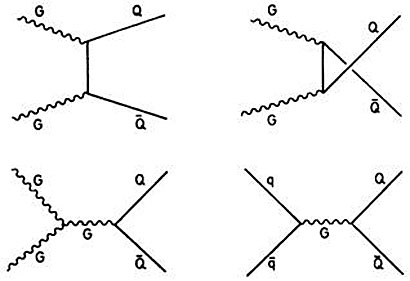
\includegraphics[width=0.45\textwidth]{Figures/Chapter1/HQDiagram.jpg}
\caption{The four lowest order tree level Feynman diagrams of heavy quark pair production are shown above.}
\label{HQProduce}
\end{center}
\end{figure}   

In general, due to their relatively momentum transfer to the medium constituents compared to mass \cite{}, they do not reach complete thermalization via multiple scattering as they traverse through the QGP. In addition, since their lifetime is much longer than the QGP lifetime, they retain their identities and record the evolution of the QGP, which makes them excellent probes. Then, they travel through the medium, hadronize into heavy flavor hadrons, and decay weakly. Their decay product are detected and identified by particles detectors.

Experimentally, from the final stage decay products, we can fully reconstruct open heavy flavor hadrons where heavy quark dynamics is encoded with different transverse momenta to study their diffusion coefficients, hadronizaton mechanism, and energy loss to probe the microscopic structure of QGP via their scattering patterns with the QGP constituents at different wavelengths. Figure \ref{HQ} below shows respectfully an event of beauty heavy quark production and hadronization in vacuum and QGP.

 \begin{figure}[hbtp]
\begin{center}
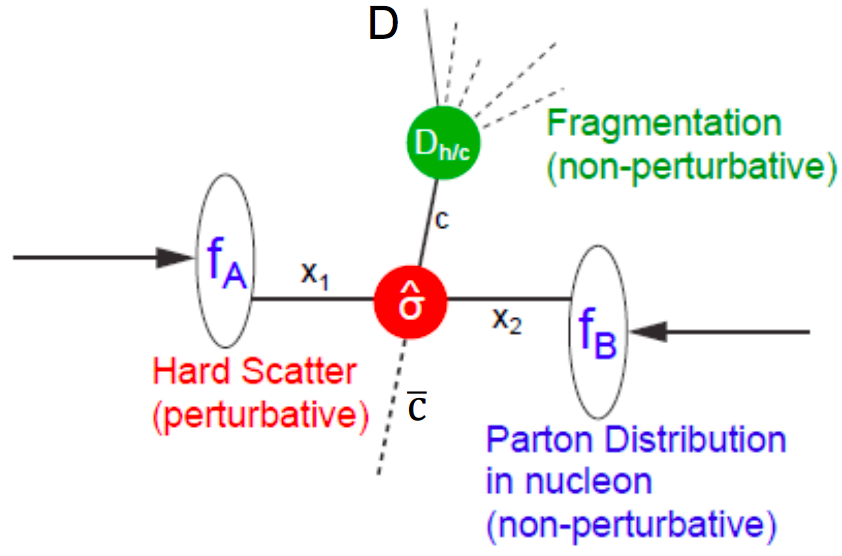
\includegraphics[width=0.46\textwidth]{Figures/Chapter1/HQVacuum.png}
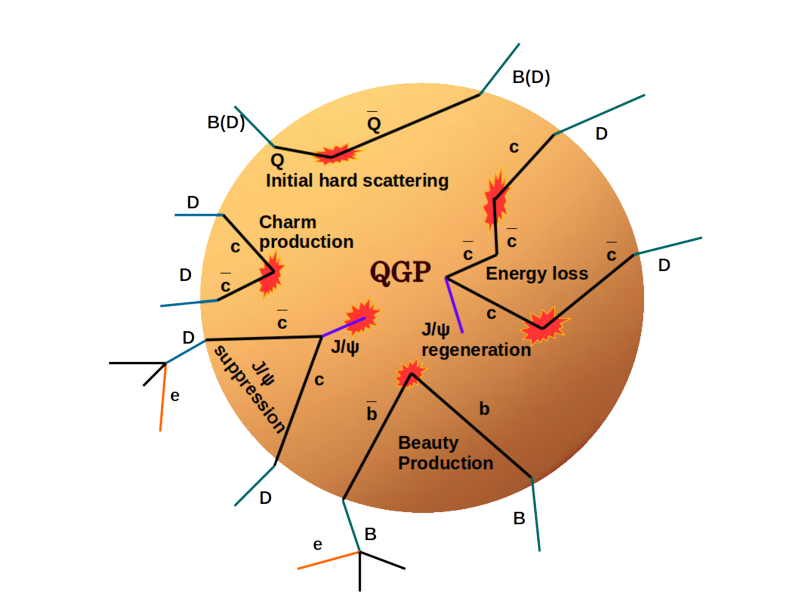
\includegraphics[width=0.48\textwidth]{Figures/Chapter1/HQQGP.png}
\caption{The schematic plots of heavy quark production and hadronization in vacuum (left) and QGP (right) are shown above.}
\label{HQ}
\end{center}
\end{figure}   


\subsection{Open Heavy Flavor Physics}

My graduate research focuses on answering the second question through the data analysis of fully reconstructed heavy flavor hadrons with the CMS experiment to understand transport properties and probe the microscopic structure of QGP. In this section, we will focus on discussing open heavy flavor physics where the only one heavy quark $Q$ is in hadron. Open heavy flavor hadrons have $\pm 1$ heavy flavor number. Quarkonia states $Q\bar Q$ are considered as hidden heavy flavor with a zero net heavy flavor quantum number. Their properties are different from open heavy flavor hadrons. We will not be discussed them in the follow subsections. 

\subsection{Heavy Flavor Physics in Vacuum}

To use heavy quark to probe the QGP created in heavy-ion collisions, we first need to understand heavy quark physics in vacuum from pp collisions. In the process $pp \rightarrow Q \bar Q$, QCD factorization theorem could be applied to study the using perturbative QCD (pQCD). Highn precision QCD calculations, including next-to-leading order (NLO), next-to-next-to-leading-order (NNLO), and Fixed-to-Next-to-the-Leading (FONLL), have been developed to describe heavy flavor production. Here, we will show FONLL calculation of the spectra of charm and beauty quarks, schematically denoted as: $\frac{d^2\sigma^Q}{p_T dp_T dy}$, in $pp \rightarrow Q  \bar Q$ at different energies \cite{FONLLRef}. Figure \ref{FONLL} shows the FONLL calculations of charm and beauty quarks spectra produced at the LHC energy for pp collisions at $\sqrt s = 5.02$ TeV.

 \begin{figure}[hbtp]
\begin{center}
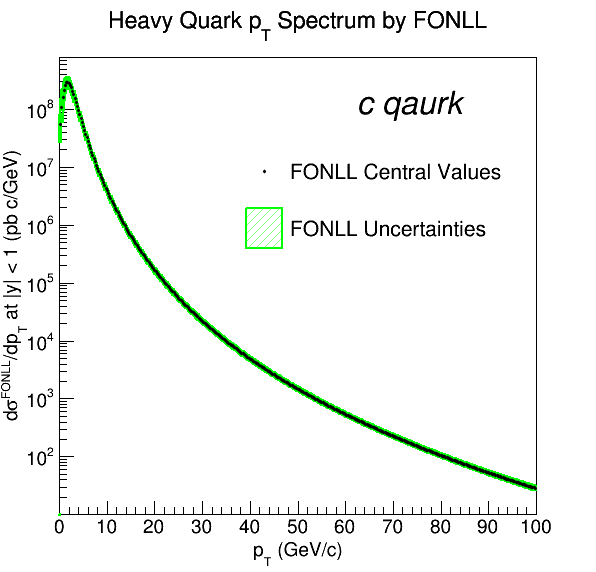
\includegraphics[width=0.45\textwidth]{Figures/Chapter1/Charm.png}
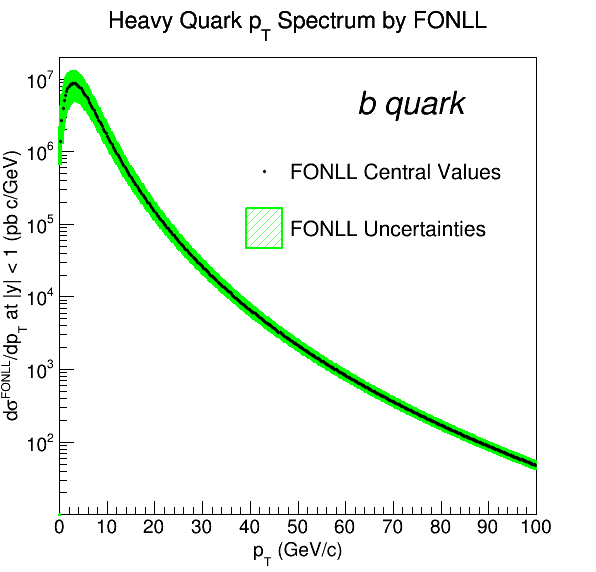
\includegraphics[width=0.45\textwidth]{Figures/Chapter1/Beauty.png}
\caption{The charm quark (left) and beauty quark (right) transverse momentum $p_T$ distribution at $\frac{d\sigma}{dp_T}$ at $|y| < 1$ from FONLL calculations are shown above.}
\label{FONLL}
\end{center}
\end{figure}   

In vacuum, heavy quarks fragment into heavy flavor hadrons $Q \rightarrow H_Q$. We can defined the parton fragmentation function $D^{H_Q}_{i}(z,\mu^2)$ where is the probability for a quark $q$ with energy $E$ fragment into a hadron with energy $zE$ ($0 < z < 1$) at the factorization scale of $\mu^2$ \cite{QCDFFunc}. According to pQCD, $D^{H_Q}_{i}(z,\mu^2)$ is universal in vacuum from $e^+e^-$, $ep$, and $pp$ collisions. Figure \ref{FFProcess} shows the scattering processes which fragmentation fraction is involved:

 \begin{figure}[hbtp]
\begin{center}
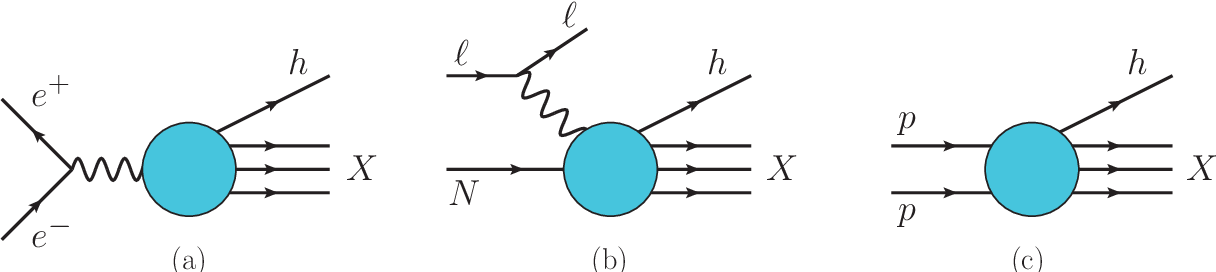
\includegraphics[width=1.0\textwidth]{Figures/Chapter1/FFProcess.png}
\caption{Single-inclusive hadron production process, where fragmentation function are involved, in (a) electron-positron annihilation, (b) deep-inelastic lepton-nucleon scattering, (c) proton-proton scattering are shown above.}
\label{FFProcess}
\end{center}
\end{figure}   

Next, we are ready to define heavy quark fragmentation fraction $f(Q \rightarrow H_Q)$. First we know, the energy

\begin{equation}
E=  \sqrt{m^2 + p_T^2 \cosh^2 y}
\end{equation}

Ignoring the mass, we have

\begin{equation}
E \simeq p_T \cosh y
\end{equation}

So energy of hadron $E^h$ that the quark with $E^Q$ fragmented to will be


\begin{equation}
E^h  = z E^Q 
\end{equation}

So we have the transverse momentum of the hadron $p_T^h$ 

\begin{equation}
p_T^{H_Q} = z p_T^Q
\end{equation}

With heavy quark spectra $ \frac{d^2\sigma^Q}{p_T dp_T dy}$ and parton fragmentation function $D_{i}^{H_Q}(z,\mu^2)$, we let


\begin{equation}
 \frac{d^2\sigma^Q}{p_T dp_T dy} = F^Q(p_T, y)
\end{equation}


Hence, for a hadron with $p_T$, the heavy quark will have $p_T/z$ with probability $D^{H_Q}_{i}(z)$ to fragment into this hadron. Therefore, the heavy flavor hadron spectra is given by:

\begin{equation}
\frac{d^2\sigma^{H_Q}}{p_T dp_T dy} = \int_{x_T}^1 F^Q(p_T/z, y) D_{i}^{H_Q}(z,\mu^2) dz
\end{equation}

Here $x_T = \frac{2p_T}{\sqrt s}$ \cite{HadronScale}.







\iffalse



From Figure \ref{FONLL} , it looks like the $p_T$ spectra of heavy quarks is overall approximately power law, particularly at high $p_T$. In fact, at a fixed $x_T$ and the center of mass angle \cite{HadronScale}, the heavy quark spectra overall demonstrates the power like behavior. In addition, assuming the spectra $F^Q(p_T,y)$ factorizes, we have
 

\begin{equation}
F^Q(p_T, y) \sim g(y) p_T^{-n}
\end{equation}

Hence,

\begin{equation}
F^Q(p_T/z, y) \sim F^Q(p_T, y)/z^{-n} = F^Q(p_T, y) z^n
\end{equation}


\begin{equation}
\frac{d^2\sigma^{H_Q}}{p_T dp_Tdy} \simeq \int_{x_T}^1 F^Q(p_T, y)  z^{n} D^{H_Q}_{i}(z) \frac{dz}{z^2} =F^Q(p_T, y)  \int_{x_T}^1  z^{n-2} D^{H_Q}_{i}(z) dz
\end{equation}



Hence, we can define the approximately constant heavy quark fragmentation fraction $f_{Q \rightarrow H_Q}$ as follows

\begin{equation}
f(Q \rightarrow H_Q) = \int_{x_T}^1 z^{n-2} D^{H_Q}_{i}(z) dz
\end{equation}

Hence, we will get 

\begin{equation}
\frac{d^2\sigma^{H_Q}}{p_T dp_T dy} = f(Q \rightarrow H_Q)  \frac{d^2\sigma^Q}{p_T dp_T dy}
\end{equation}

\fi

Now if we consider a factorization scaling near the heavy quark mass $\mu^2 \rightarrow m_Q^2$, according to PDG reference \cite{AlphaTheoEx}, solving the leading evolution equation, heavy quark fragmentation function $D_Q^{H_Q}(z)$ is in a form of delta function and light quark $q$ and gluons $g$ ($i = g, q$) will not contribute to produce heavy flavor hadrons. Hence, we could right

\begin{equation}
D^{H_Q}_{q,g}(z,\mu^2)|_{\mu^2=m_Q^2} = 0
\end{equation}

\begin{equation}
D^{H_Q}_{Q}(z,\mu^2)|_{\mu^2=m_Q^2} = f(Q \rightarrow H_Q) \delta(1 - z)
\end{equation}

Here $f({Q \rightarrow H_Q})$ is the heavy quark fragmentation fraction and stands for the probability of a heavy quark $Q$ hadronize into an open heavy flavor hadron $H_Q$. Indeed, according to the momentum sum rule constraint of the parton fragmentation function \cite{QCDFFunc}

\begin{equation}
\sum_{H_Q} \int_0^1 z D^{H_Q}_{Q}(z,\mu^2) dz = 1
\end{equation}

\begin{equation}
\sum_{H_Q} \int_0^1 z f(Q \rightarrow H_Q) \delta(1 - z) dz = 1
\end{equation}

\begin{equation}
\sum_{H_Q} f(Q \rightarrow H_Q) = 1 
\end{equation}

This verifies that the sum of heavy quark fragmentation fraction over all heavy flavor hadrons is equal to 1. Next, we have 


\begin{equation}
\frac{d^2\sigma^{H_Q}}{p_T dp_T dy} = \int_{x_T}^1 F^Q(p_T/z, y) D_{i}^{H_Q}(z,\mu^2) dz =  \int_{x_T}^1 F^Q(p_T/z, y) D^{H_Q}_{Q}(z,m_Q^2) dz 
\end{equation}

Thus,

\begin{equation}
\frac{d^2\sigma^{H_Q}}{p_T dp_T dy}  = \int_{x_T}^1 F^Q(p_T/z, y) f(Q \rightarrow H_Q) \delta(1 - z) dz =  f(Q \rightarrow H_Q)  F^Q(p_T, y)
\end{equation}

Hence, we have 

\begin{equation}
\frac{d^2\sigma^{H_Q}}{p_T dp_T dy} = f(Q \rightarrow H_Q) \frac{d^2\sigma^{Q}}{p_T dp_T dy}
\end{equation}

This means that the open heavy flavor hadron spectra $\frac{d^2\sigma^{H_Q}}{p_T dp_T dy}$ is essentially proportional to the heavy quark spectra $\frac{d^2\sigma^{Q}}{p_T dp_T dy}$ with heavy quark fragmentation fraction $f(Q \rightarrow H_Q)$ the as the coefficient of proportionality. Experimentally, charm and beauty fragmentation fractions have been measured at LEP, HERA, and the LHC and documented in PDG \cite{AlphaTheoEx}. The fragmentation fraction is often treated roughly a constant independent to $p_T$, $y$, and $\sqrt s$ and is assumed to be universal in $e^+e^-$, $ep$, and $pp$ collisions systems \cite{AlphaTheoEx}. 

In terms of being a constant, according LHCb $pp$ results \cite{LHCbFF}, it appears that the fragmentation fraction has significant $\sqrt s$ and $p_T$ dependence while no significant $y_B$ (or $\eta_B$) dependence is observed. Figure \ref{BeautyFFLHCb} shows the beauty quark fragmentation fraction: $f_u = f(b \rightarrow B^+)$, $f_d = f(b \rightarrow B^0)$, and $f_s = f(b \rightarrow B_s^0)$

 \begin{figure}[hbtp]
\begin{center}
\includegraphics[width=0.60\textwidth]{Figures/Chapter1/LHCbFFs.png}
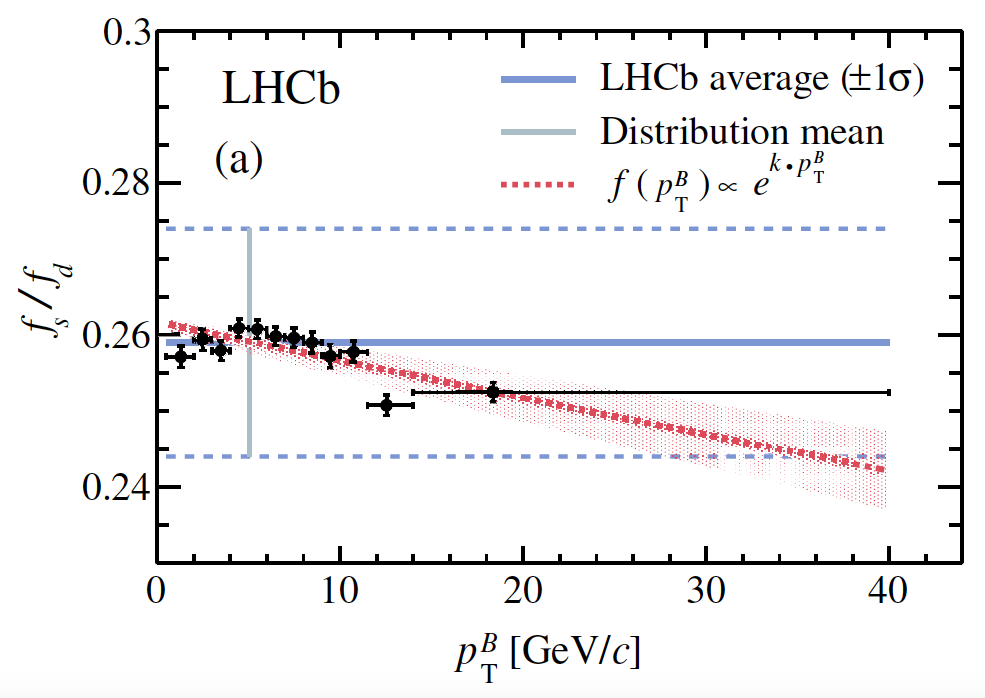
\includegraphics[width=0.60\textwidth]{Figures/Chapter1/LHCbFFpT.png}
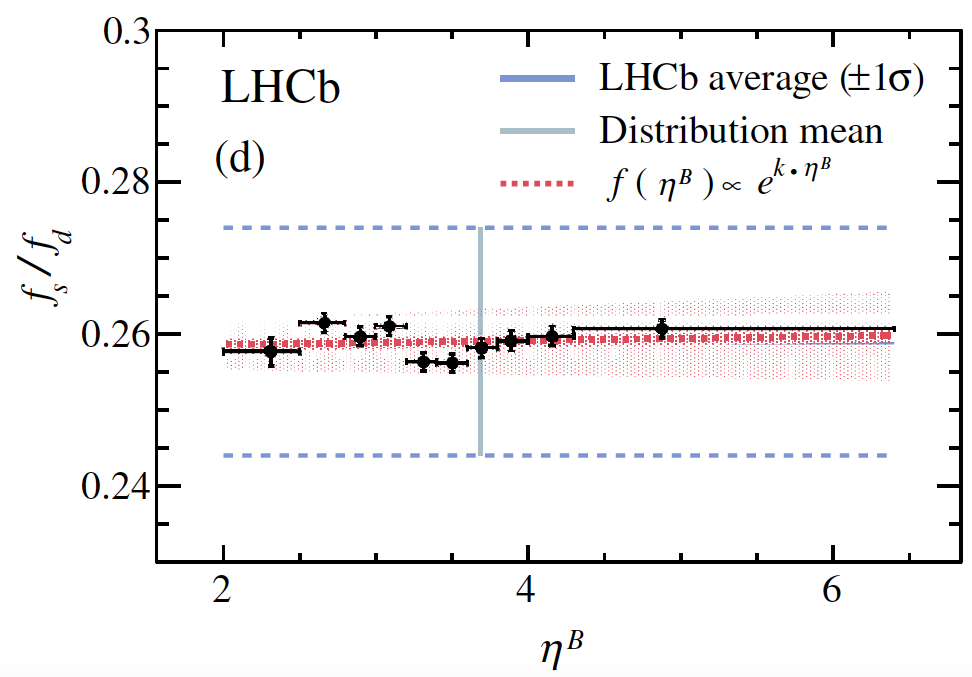
\includegraphics[width=0.60\textwidth]{Figures/Chapter1/LHCbFFy.png}
\caption{ $R$, the corrected yield ratio of $B^0_s/B^+$, as a function the $pp$ collision energy $\sqrt s$ (top), the $f_s/f_d$ ratio as a function $p_T$ (middle), and the $f_s/f_d$ ratio as a function $\eta_B$ (bottom), from the LHCb experiment are shown above.}
\label{BeautyFFLHCb}
\end{center}
\end{figure}   


In terms of universality, according to Strangeness Quark Matter Conference (SQM) in 2021, a hadronization universality breaking is observed from the ALICE experiment at the LHC \cite{GMISQM}. Figure \ref{CharmFFALICE} shows the hadronization universality breaking reported by the ALICE experiment in SQM 2021

 \begin{figure}[hbtp]
\begin{center}
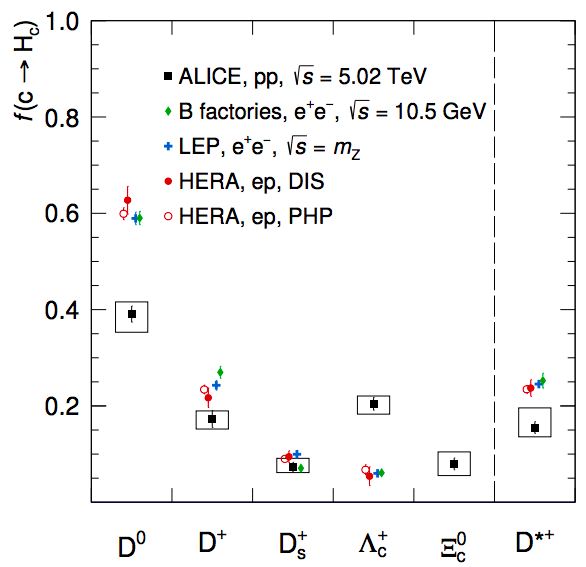
\includegraphics[width=0.52\textwidth]{Figures/Chapter1/ALICECharmFF.png}
\caption{The charm quark fragmentation fraction to different charm hadrons species in $e^+e^-$, $ep$, and $pp$ collisions are presented above. From the ALICE experiment, we can clearly see that the fragmentation fraction of $D^0$ has drop by about 40\% while the $\Lambda_c^+$ has enhanced by about a factor of 4. Therefore, the hadronization universality is clear broken at the LHC energy in the charm sector.}
\label{CharmFFALICE}
\end{center}
\end{figure}   

Further investigations of these results are currently ongoing. However, we will not expand the discussions here. Now, equipped with the understanding of heavy flavor physics in vacuum from $pp$ collisions as a reference, we are ready to use heavy quarks to probe the inner workings of QGP created in heavy-ion collisions. 

\subsection{Heavy Quark Diffusion}

In the limit of low $p_T$ or equivalently long wavelength, for heavy quarks inside the QGP medium, their elastic collision cross section dominates. In elastic $Q q \rightarrow Q q$ process in the thermally equilibrated QGP medium, heavy quarks has the relatively small momentum transfers of the order of the temperature compared to the heavy quark mass: $m_Q > |k| \simeq T$. Considering the mean free time of HQ in the QGP medium is about $\tau \sim 0.44 fm/c$ \cite{HQTau}. Therefore, the number of scattering of heavy quarks in the QGP medium is about $n \sim \frac{\tau_{QGP}}{\tau_{HQ}} \simeq 23 \sim O(10)$.

Now, we can consider a simple binomial process to model the diffusion of heavy quark in the QGP medium. Therefore, assuming the momentum of the heavy quark at $t = 0$ is $p$, after the time $\tau_{HQ}$, one scattering happens. The momentum of the heavy quark at $t = \tau_{HQ}$ either $p + k$ or $p - k$. Each has $1/2$ probability. Next, after another $\tau_{HQ}$, another scattering happens. The momentum of the heavy quark at $t = \tau_{HQ}$ either $p + 2k$, $p$ or $p - 2k$ with $1/4$, $1/2$, and $1/2$ probability respectfully. Therefore, the standard deviation of binomial process $\sigma_p = \frac{\sqrt{n}}{2} k$. If we take $n = 25$, $\sigma_p = 2.5k \simeq 2.5 T_{QGP} =$ 0.4 GeV. Experimentally, we consider a heavy quark with momentum about $p  > $ 1.5 GeV/c $>> \sigma_p$. 






We could see that the heavy quark transverse momentum is well above 1 GeV/c. Hence, such heavy quarks still retain a lot of memory about its initial conditions after multiple small scattering with QGP medium. Hence, in these conditions, heavy quark undergoes Brownian-like motion in the QGP medium \cite{HQReview}. Their motion in the QGP medium could be characterized by the Planck-Fokker Equation, which could be schematically written as follows \cite{HQRaff}:

\begin{equation}
\frac{\partial}{\partial t} f_q(t, \vec{p}) = \frac{\partial}{\partial p_{i}} \{ A_i(\vec p) f_q(t,\vec{p}) + \frac{\partial}{\partial p_j}[B_{ij}(\vec{p})f_q(t,\vec{p}) ] \}
\end{equation}

Here, $f_q(t,\vec{p})$ is the heavy quark phase space distribution function. If we ignore modification of the cold nuclear matter effect on the heavy quark initial production spectra, then in heavy-ion collision:

\begin{equation}
F^Q( t = 0,p_T) \propto \frac{d\sigma_{FONLL}}{p_Tdp_T}
\end{equation}


The transport parameters $A_i(\vec{p})$ is related to the thermal relaxation rate and $B_{ij}(\vec{p})$ is related to the momentum diffusion of heavy quark \cite{HQReview}. The heavy quark special diffusion coefficient $D_s$ is related to the transport parameter as follows:

\begin{equation}
D_s = \frac{T} {m_Q A(p=0)}
\end{equation}

$D_s$ characters the fundamental property of the QGP $\frac{\eta}{s}$ via the relationship 

\begin{equation}
2 \pi T D_s \simeq \frac{\eta}{s}
\end{equation}

More detailed studies has been carried out to examine heavy quark coupling strength and quantify the information heavy quarks carry as they traverse through the QGP medium \cite{HQJamie}.


\subsection{Heavy Quark Energy Loss}

In the limit of high $p_T$ or equivalently short wavelength, inelastic cross section starts to dominate \cite{}. Heavy quarks lose a substantial amount of energy as they travel fast through the QGP medium \cite{HQELossFirst}. In a simplified schematization, there are two different pictures that describe the energy loss mechanism of heavy quark in the QGP medium. In the pQCD picture, the coupling of the constituents of the QGP is assumed to be weak. Therefore, the QGP is made of weakly coupled quasiparticles. Heavy quarks scatter off the constituents incoherently when propagating through the QGP medium. There are two energy loss mechanisms: collisional energy loss and radiative energy loss \cite{HQRaff}. The collisional energy loss is given by $-\frac{dE}{dx} = \kappa_{coll}T^2$ and the radiative energy loss is given by  $-\frac{dE}{dx} = \kappa_{rad}T^3x$ \cite{HQCollELoss,HQRadELoss}. Figure \ref{HQELosspQCD} shows schematically heavy quark energy loss mechanism in the QGP medium



 \begin{figure}[hbtp]
\begin{center}
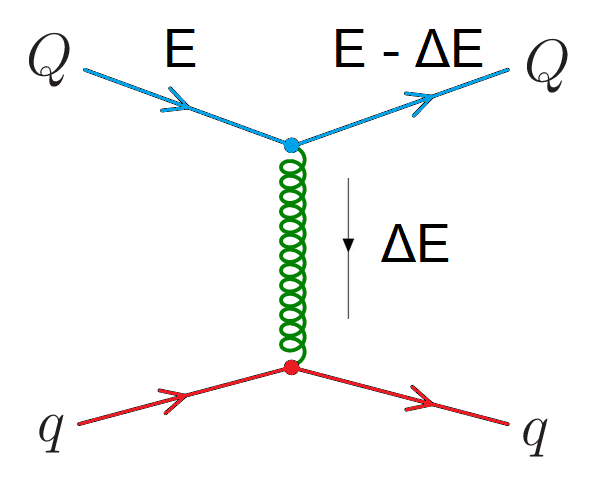
\includegraphics[width=0.35\textwidth]{Figures/Chapter1/Collisional.png}
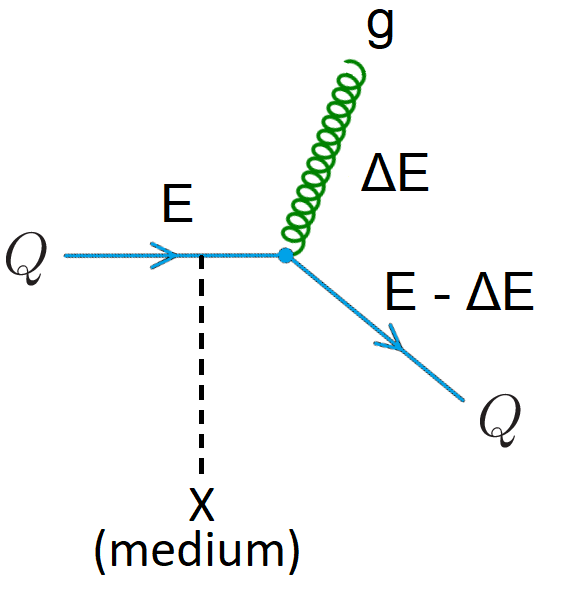
\includegraphics[width=0.35\textwidth]{Figures/Chapter1/Radiative.png}
\caption{The schematic demonstration of the pQCD picture: collisional energy loss (left) and radiative energy loss (right) of heavy quarks in the QGP medium are shown above.}
\label{HQELosspQCD}
\end{center}
\end{figure}   

The other picture, AdS/CFT, takes the strong coupling limit. In this picture, QGP behave like liquid and heavy quarks scatter off the constituents coherently in the QGP medium. The AdS/CFT model applies holographic drag force \cite{ADSCFTDrag} to calculate the energy loss of heavy quark \cite{HQHoloELoss} in the QGP medium

 \begin{figure}[hbtp]
\begin{center}
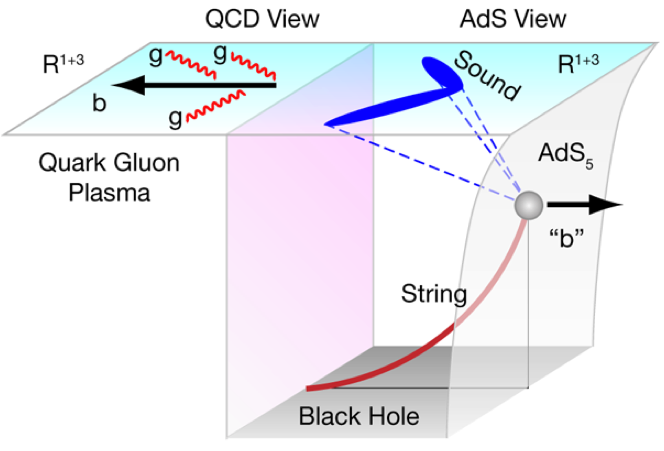
\includegraphics[width=0.45\textwidth]{Figures/Chapter1/ADSCFT.png}
\caption{The schematic demonstration of ADS/CFT picture: the energy loss of a quark in the QGP medium holographically due ADS/CFT drag force.}
\label{ADCCFT}
\end{center}
\end{figure}  

In pQCD picture, in the limit of $p_T \rightarrow \infty$, similar to electron Bremsstrahlung via QED radiation in the matter \cite{Brems}, for a heavy quark traveling through the QGP medium, its radiative energy loss via soft gluon radiation will dominate. The soft gluon radiation spectrum by a parton in the QGP medium is given by \cite{DEADCONE}

\begin{equation}
dP = \frac{\alpha_S C_{F}}{\pi} \frac{d\omega}{\omega}\frac{k_{\perp}^2 dk_{\perp}^2}{(k_{\perp}^2  + \omega^2\theta_0^2)^2}
\end{equation}

Where 

\begin{equation}
\theta_0 \equiv \frac{m}{E}
\end{equation}

Here, $\omega$ is the energy of the gluon and $k_{\perp}$ is the transverse momentum of the gluon, $C_F$ is color factor (Casimir) which is $3$ for gluons with one color and one anti-color charges and $4/3$ for quarks with one color charge. From Eq 1.84 above, a suppression of radiation at a small angle $0 - \theta_0$ is observed. This is effect is known as the dead cone phenomenon \cite{DEADCONE}. We also know that from from Eq 1.85, that as $m$ increases, the dead cone angle $\theta_0 = \frac{m}{E}$ will decrease. Figure \ref{DeadConePic} schematically shows a charm quark radiate gluon in the medium with a dead cone in the small angle:

 \begin{figure}[hbtp]
\begin{center}
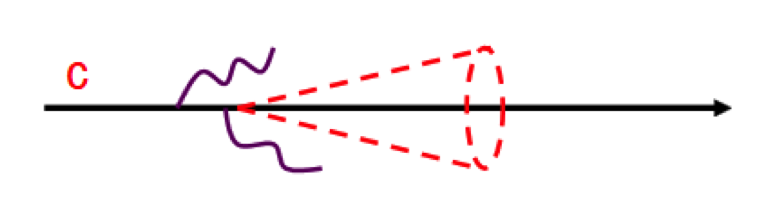
\includegraphics[width=0.85\textwidth]{Figures/Chapter1/CharmDeadCone.png}
\caption{The schematic demonstration of a charm quark radiate and suppression in small angle due to the dead cone effect in the QGP medium is shown above.}
\label{DeadConePic}
\end{center}
\end{figure}  

Since we have the follow mass hierarchy for quarks and gluons:

\begin{equation}
m_g < m_q < m_c < m_b
\end{equation}

We should expect the energy loss to follow

\begin{equation}
\Delta E_g > \Delta E_q > \Delta E_c >  \Delta E_b
\end{equation}

We call the inequality above to be the flavor dependence of energy loss, which is an important feature of heavy quark energy loss mechanism in the QGP medium. The studies of heavy quark energy loss mechanism in QGP will help us determine the fundamental jet transport coefficient $\hat q$ that characterizes the scattering power of the medium \cite{HQReview}. which relates to the mean free path and the momentum diffusion coefficient of heavy quarks \cite{qhatStudy}. The determination of $\hat q$ will be crucial for us decipher the inner workings of the QGP \cite{JetTransProbe}.

\subsection{Heavy Quark Hadronization}

After heavy quarks traverse through the medium, it will hadronize into heavy flavor hadrons, which could be fully reconstructed from their final state decay products in experiments. As described in section 1.2.7, in general, hadronization is non-perturbative. Considering heavy quark dynamics and apply hadronization models, physicists develop theoretical models to describe heavy quark hadrochemistry. Below, I will present two model candidates, the Texas A\&M University (TAMU) Model \cite{TAMUModel} and the Model developed from Cao et. al. \cite{CaoSunKo}, to describe beauty quark production and hadronization in vacuum:


\subsubsection{TAMU Model}

The TAMU Model uses a thermodynamic T-matrix formulism in terms of ``ladder diagrams'' to compute the heavy quark in-medium scattering amplitude and determine the non-perturbative transport parameters $A_i$ and $B_{ij}$ in the Planck-Fokker equation shown in Eq 1.81 \cite{TAMUModel}. Figure \ref{LadderDiagram} shows schematically the ``ladder diagram'' describing the dynamic evolution of a heavy quark in the QGP medium 

 \begin{figure}[hbtp]
\begin{center}
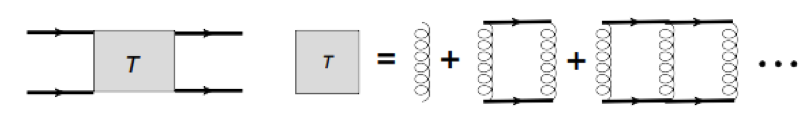
\includegraphics[width=1.0\textwidth]{Figures/Chapter1/LadderDiagram.png}
\caption{The ladder diagram used by the TAMU model to describe heavy quark diffusion in the QGP medium is shown schematically above.}
\label{LadderDiagram}
\end{center}
\end{figure}  

The input of T-matrix uses a lattice QCD potential \cite{LQCDTAMU} corrected with relativistic effects to model the non-perturbative interaction between heavy quarka and partons in the medium and make it consistent with HF spectroscopy in vacuum to determine the thermal relaxation rate coefficient $A_i(p,T)$. Only elastic collisional energy loss is included in the calculation. Resonance recombination model of heavy quark with a light quark nearby is applied to describe heavy quark hadronization \cite{RRM1}. Finally, effective hadronic scattering amplitudes is used to heavy flavor hadronic rescattering with other hadrons before kinetic freezout stage. The background parton composition and kinematics are modeled by the standard hydrodynamic simulations of the bulk medium in nuclear collisions

\subsubsection{Cao, Sun, Ko Model}

The Cao, Sun, Ko Model use an advanced Langevin-hydrodynamics approach \cite{CaoLH1,CaoLH2} incorporating both elastic and inelastic energy loss of heavy quarks inside the dynamical QGP medium. The equation below schematically shows relativistic Langevin equation to simulate heavy quark dynamics in the QGP medium


\begin{equation}
\Delta \vec{p} = - \gamma \frac{T^2}{M} \vec{p} \Delta t + \vec{\xi}(t) 
\end{equation}

And

\begin{equation}
\Delta \vec{x} = - \frac{\vec{p}}{E} \Delta t
\end{equation}

The noise is modeled by the Gaussian diffusion function 

\begin{equation}
P(\vec{\xi}) \propto \exp[\frac{\vec{\xi}^2}{2D_p \Delta t}]
\end{equation}

The dimensionless $\gamma$ factor is defined as

\begin{equation}
\gamma = \frac{M}{\tau_{HQ} T^2}
\end{equation}


A comprehensive coalescence model with strict energy-momentum conservation and PYTHIA fragmentation simulation \cite{PYTHIAFrag} with the default Peter fragmentation function, where the coalescence probability is determined from resonant scattering rate of heavy quarks in the QGP according to the resonant recombination model \cite{RRM1,RRM2}, are applied to model heavy quark hadronization.

In addition to TAMU Model and Cao, Sun, Ko Models, there are many other theoretical models that describe heavy quark hadrochemistry in heavy-ion collisions. Nevertheless, due to the large discrepancies between hadronization models, which significant limits the heavy-ion community to interpret the heavy flavor data. Therefore, experimentalists precisely measure heavy flavor observables and provide constrains for theoretical models.


 
\subsubsection{Equal Velocity Recombination Model}

In this model, the transverse momentum distribution of initially produced heavy quark is calculated by FONLL \cite{QCMModel}. The jet quenching effect in heavy-ion collisions is considered according to $R_{AA}$ measurement of $B^+$. The transverse momentum distributions of light-flavor quarks are obtained from data of light hadrons in the model. This model is particular designed to study low $p_T$ and mid-rapidity charm quarks produced at the LHC energy. It considers the equal-velocity combination of bottom quark with light-flavor anti-quarks  to form B mesons, a framework based on of co-moving quark recombination model (QCM).

\iffalse



\subsection{Experimental Observables}

Therefore, physicists propose many experimental observables to study open heavy flavor physics and test theoretical models in heavy ion collisions. Traditionally, heavy flavor hadron $v_2$, $R_{AA}$, and yield ratio are extensively studied. 

\textbf{Heavy Quark Diffusion: $v_2$}

In the QGP medium, heavy quark diffused by the color force and multiple scatter with medium constituents, which could generate sizable azimuthal anisotropy $v_2$ \cite{HQReview}. Experimentally, we scale the $v_2$ and the hadron kinetic energy $K_T = \sqrt{m^2 + p_T^2} - m^2$ of heavy quarks with $n_q$ according to the Number of Constituent Quark (NCQ) Scaling in quark coalescence model \cite{NCDScaling}. Figure \ref{HQV2} shows the comparison of the $v_2/n_q$ as a function of $K_T/n_q$ of $D^0$ ($c\bar u$) meson with light flavor hadrons with STAR experiments at RHIC \cite{STARD0v2} and the CMS experiment at LHC \cite{CMSD0v2}.


\begin{figure}[hbtp]
\begin{center}
\includegraphics[width=0.50\textwidth]{Figures/Chapter1/STARv2.png}
\includegraphics[width=0.485\textwidth]{Figures/Chapter1/CMSv2.png}
\caption{The NCQ scaled $D^0$ $v2/n_q$ vs $K_T/n_q$ and the comparison light hardons measured by the STAR experiment at RHIC (left) and the CMS experiment at LHC (right) are shown above.}
\label{HQV2}
\end{center}
\end{figure}   

We could see a reasonably good NCQ scaling behavior of $D^0$ meson with other light flavor hadrons, which suggests sizable collectivity of charm quarks in the QGP medium.

\textbf{Heavy Quark Energy Loss Mechanism: $R_{AA}$}

As we mentioned previously, the nuclear modification factor $R_{AA}$ of heavy flavor hadrons as a function of $p_T$ could quantify the energy loss of quarks via the shift of the $p_T$ spectra to the left in $AA$ collisions compared to $pp$ collisions. Figure \ref{HQRAA} $R_{AA}$ heavy and flavor hadrons measured with experiments at RHIC and LHC.

\begin{figure}[hbtp]
\begin{center}
\includegraphics[width=0.47\textwidth]{Figures/Chapter1/STARRAA.eps}
\includegraphics[width=0.47\textwidth]{Figures/Chapter1/CMSRAA.png}
\caption{The $D^0$ $R_{AA}$ vs $p_T$ with the STAR experiment in 0 - 10\%, 10 - 40\%, and 40 - 80\% centrality at RHIC and the $D^0$, $B^+$, non-prompt $J/\psi$ and charged hadrons $R_{AA}$ vs $p_T$ at at 0 - 100\% centrality with the CMS experiment at LHC are shown above.}
\label{HQRAA}
\end{center}
\end{figure}   

We could see that $R_{AA}$ of $D^0$ and $B^+$ are both below 1, which suggest charm and beauty quarks lose a significant fraction of energy to the QGP medium. As $p_T$ increases, the $R_{AA}$ of light and heavy flavor hadrons converge to the same value and approach 1, which Lorentz $\gamma$ factor come into play where the mass of the hadron become irrelevant. In addition, the CMS results above indirectly agree with the expectation of the flavor dependence of energy loss: $R_{AA}^{h} < R_{AA}^{D} < R_{AA}^{B} < 1$. With both $R_{AA}$ and $v_2$, we can constrain theoretical models and understand the interaction mechanism of heavy quarks with the QGP medium.

\textbf{Heavy Quark Hadronization: $H_s/H^0$ and $\Lambda_{Q}/H^{0}$}

According to the theoretical reviews of heavy quarks hadrochemistry in heavy-ion collisions \cite{StrangetoLight,BaryontoMeson}, the strange-to-non-strange meson ($H_s/H^0$) and baryon-to-meson ($\Lambda_{Q}/H^{0}$) ratios are excellent observables to test hadronization models. Figure \ref{HadroPlotCharm} shows the fully reconstructed $\Lambda_C^+/D^0$ ratio measured by the STAR and CMS experiments

\begin{figure}[hbtp]
\begin{center}
\includegraphics[width=0.52\textwidth]{Figures/Chapter1/STARLambdaCD0.png}
\includegraphics[width=0.47\textwidth]{Figures/Chapter1/ALICELambdaCD0}
\caption{The fully reconstructed $\Lambda_C^+/D^0$ ratio in pp and heavy-ion collisions measured by the STAR experiment at RHIC (left) and the CMS experiment at LHC (right) are shown above.}
\label{HadroPlotCharm}
\end{center}
\end{figure}   

We can see that in general, $\Lambda_C^+/D^0$ ratio in heavy-ion collisions lies above its ratio in $pp$ collisions. Moreover, there are many different theoretical predictions agree reasonably well with the experiments due to the large uncertainties. More precise $\Lambda_C^+/D^0$ measurements will be desired in order to constrain theoretical models.

In addition to $v_2$, $R_{AA}$, and $\Lambda_{Q}/H^{0}$, some modern observables with more differentiation such as the hadron-hadron correlation and heavy flavor jet substructure measurements have been recently carried out \cite{DDbar,DJet}. 

Hence, with the motivation to understand the hadronization mechanism of heavy quarks and investigate the inner workings of the QGP, I propose to carry out open heavy flavor physics measurements. In this thesis, I will focus on the measurement of the experimental observable $B^0_s/B^+$ ratio from fully reconstructed $B^0_s$ and $B^+$ mesons (and their anti-particles) via decay channels of $B^0_s \rightarrow J/\psi \phi \rightarrow \mu^+ \mu^- K^+ K^-$ and $B^0_s \rightarrow J/\psi K^+ \rightarrow \mu^+ \mu^- K^+$ in pp and PbPb collisions with the CMS experiment at the LHC to study the beauty production and hadronization mechanism in vacuum and QGP. 



\fi

%% This is an example first chapter.  You should put chapter/appendix that you
%% write into a separate file, and add a line \include{yourfilename} to
%% main.tex, where `yourfilename.tex' is the name of the chapter/appendix file.
%% You can process specific files by typing their names in at the 
%% \files=
%% prompt when you run the file main.tex through LaTeX.
\chapter{The CMS Detector}

\section{Overview}

The Compact Muon Solenoid (CMS) Detector is a general purpose high-energy physics detector located 100 meters underground on the French side of the LHC \cite{CMSDetector}. Overall, the complete detector is 21 m long, 15 m wide and 15 m high with a weight of 14 kiloton, heavier than the Eiffel Tower in Paris. It functions as a giant, high-speed camera, taking 3D ``photograph'' of particle collisions from all directions up to 40 million times each second. Figure \ref{CMSRealPic} shows the photo taken for the CMS detector at the underground collision hall.

\begin{figure}[hbtp]
\begin{center}
\includegraphics[width=0.80\textwidth]{Figures/Chapter2/CMSRealPic.jpg}
\caption{The front view of the CMS detector at the underground collision hall is shown above.}
\label{CMSRealPic}
\end{center}
\end{figure} 

The CMS detector is made of sub-detectors including silicon strip and pixel trackers, the preshower made of silicon strips, the crystal electromagnetic calorimeter (ECAL), the superconducting solenoid with 3.8 T of magnetic field strength, the inner hadronic calorimeter (HCAL), the steel returning yoke to enhance the magnetic field strength, the outer hadronic calorimeter, the muon chambers, and the forward hadronic calorimeter \cite{CMSDetector}. Figure \ref{CMSDecPic} shows schematic view of the CMS detector

\begin{figure}[hbtp]
\begin{center}
\includegraphics[width=0.80\textwidth]{Figures/Chapter2/CMSDecPic.jpg}
\caption{The schematic view of the CMS detector with brief descriptions of all its components is shown above. Image from \cite{HiggsCMS}}
\label{CMSDecPic}
\end{center}
\end{figure} 

The CMS detector is built, operated, and maintained by the CMS Collaboration. The CMS Collaboration consists of over 4000 members including scientists, engineers, technicians, students, and administrative assistants from 200 institutes and universities in 40 countries around the world. Physicists take data from the CMS detector and share data with each other with online system. The data are store in tapes and kept at different institutions. Members of the CMS experiment collaborate with each other on detector studies and data analysis to produce important scientific results and have published in more than 1000 papers in internationally recognized journals.

In the following sections, I will describe in more details the CMS experiment including the trigger system for data acquisition, the tracking system to track charged particles, the muon system for muon detection, identification, and reconstruction, and the calorimeter system to measure the energy of the particles.

\section{Triggers}

The CMS experiment develops triggers to acquire experimental data \cite{CMSTrigger}. Its main purpose is to select events of potential physics interests from approximately one billion events per second the particles collisions at the LHC. The CMS trigger system consists of two levels of triggers: hardware level 1 (L1) trigger and the software high level trigger (HLT). Different triggers encoded in the L1 and HLT are designed and fire to collect datasets for specific physics studies.

\subsection{L1 Trigger}

In the CMS experiment, an event is defined as a snapshot of one collision at the LHC. In the L1 trigger, physicists develop algorithms according to detector electronics response to decide if an event is accepted or rejected within the L1 trigger latency time. Figure \ref{L1Overview} shows the schematic overview of L1 trigger making its decision online to select events based on the information from the calorimeter and muon systems.


\begin{figure}[hbtp]
\begin{center}
\includegraphics[width=0.50\textwidth]{Figures/Chapter2/L1Overview.png}
\caption{The figure above demonstrates how the CMS L1 hardware trigger function schematically.}
\label{L1Overview}
\end{center}
\end{figure} 

In the interest of heavy-ion studies, physicists develop a set of dedicated triggers algorithms in the L1 trigger to build datasets. The minimum biased (MB) trigger is designed to collect minimum bias data for elliptic flow, $D^0$ meson, and charged particle multiplicity analyses while the single muon trigger is designed to select events muons for heavy flavor and electroweak physics analyses. We will describe the MB trigger since we will need to use it to determine the number of MB events in our analysis.

\subsection{MB Trigger}

By definition, an MB event corresponds to a non-single diffractive inelastic interaction \cite{MBTrigger}. A totally inclusive trigger, or called zero bias (ZB) trigger, corresponds to a randomly reading out from the detector whenever a collision is possible. MB trigger is algorithm to determine interesting MB events based on the response from forward HCAL located at $3 < |\eta| < 5$. It is put a fixed analog to digital converter (ADC) threshold in the HCAL response to reject background noise and collect MB events from ZB trigger. There is also an essentially linear relation between the maximum ADC with the actual energy response of the forward HCAL. Figure \ref{HFADC} shows the ADC distribution and HF energy as a function of ADC in 2018 PbPb run.

\begin{figure}[hbtp]
\begin{center}
\includegraphics[width=0.45\textwidth]{Figures/Chapter2/AllADC.png}
\includegraphics[width=0.45\textwidth]{Figures/Chapter2/HFvsADC.png}
\caption{In the CMS 2018 PbPb Run 326791, the ZB data (red), Empty Bunches (blue), and MB data (green) ADC distributions (left), and the HF energy according to the charge collected as a function of ADC (right) are shown above. We can see that the HF energy  is about (0.5 - 1) conversion factor to the ADC.}
\label{HFADC}
\end{center}
\end{figure} 

The MB trigger consist ``MB OR'', which requires the ADC threshold on either one of the forward HCAL (HF) out of both forward ECAL in both positive and negative sides, and ``MB AND'',  which requires the ADC threshold on both of HFs out of both forward ECAL in both positive and negative sides. Figure \ref{2018PbPbMB} shows the L1 MB trigger analysis of Run 326791 in the 2018 CMS PbPb data taking 

\begin{figure}[hbtp]
\begin{center}
\includegraphics[width=0.45\textwidth]{Figures/Chapter2/MaxADC.png}
\includegraphics[width=0.45\textwidth]{Figures/Chapter2/MBTrgEffADC.png}
\caption{In the CMS 2018 PbPb Run 326791, the ZB data (red), Empty Bunches (blue), and MB data (green) maximum ADC distributions (left) and the efficiencies of MB OR (blue) and MB AND (red) as a function ADC threshold (right) are shown above.}
\label{2018PbPbMB}
\end{center}
\end{figure} 

In the 2018 CMS PbPb data taking, to reject the noisy background, the max ADC of each event is required to be greater than 15 with MB AND along with the HLT trigger of at least one pixel track are applied to select MB events, as seen above from Figure \ref{2018PbPbMB} in the max ADC distribution of MB evens in green. A total number of about 2.4 billion MB events corresponding to a luminosity about 1.7 $nb^{-1}$ have been collected by CMS during the 2018 LHC PbPb run from November to December 2018. Figure \ref{MBStat} shows the MB events and corresponding luminosity as a function day throughout the 2018 CMS PbPb data taking period

\begin{figure}[hbtp]
\begin{center}
\includegraphics[width=0.55\textwidth]{Figures/Chapter2/MBStat.pdf}
\caption{The figure above shows the total number of 20 PbPb MB events from and corresponding luminosity how the as a function Run ID from November 15 to December 2 2018.}
\label{MBStat}
\end{center}
\end{figure} 


\subsection{Centrality Efficiency with MB Trigger}

In addition to overall efficiency vs the ADC with the MB trigger, we also study the centrality efficiency with different ADC thresholds. Figure \ref{EffCent} shows the centrality as a function of efficiency using MB OR and MB AND with different thresholds

\begin{figure}[hbtp]
\begin{center}
\includegraphics[width=0.55\textwidth]{Figures/Chapter2/EffCent.png}
\caption{The efficiency vs centrality with ADC > 16 for MB OR (blue) and MB AND (green) are shown above.}
\label{EffCent}
\end{center}
\end{figure} 

Because other physics trigger are mainly based on the MB datasets, in the physics analyses using 2018 CMS PbPb datasets, it is recommended to remove the very peripheral centrality range from 90 - 100\%, which is not fully efficient (efficiency $<$ 100\%). Therefore, the most of the CMS heavy-ion physics results using the 2018 PbPb dataset will be presented in the centrality range of 0 - 90\%.

\subsection{HLT Trigger}

The HLT software trigger is an array of commercially available computers running high-level physics algorithms \cite{CMSTrigger}. Unlike the online L1 hardware trigger which runs on-the-go during the data taking process, HLT is an offline software trigger that runs after the data are acquired. In the HLT trigger, more sophisticated analyses are performed to determine if the event is accepted or rejected for a specific dataset. The event data are stored locally on disk and eventually transferred to downstream systems, the CMS Tier-0 computing center, for offline HLT processing and permanent storage \cite{CMSTrigger}. There are many trigger paths in the HLT such as the high multiplicity trigger to specifically collect events with many tracks, the D meson trigger to select high $p_T$ D mesons, and the dimoun trigger to enrich Drell-Yen events, are designed and encoded in the HLT trigger. In the following, we will describe the dimuon trigger in details because the dimuon dataset will be used to fully reconstruct B mesons in this thesis. 

\subsection{DiMuon Trigger}

The dimuon trigger, as it is named, is a trigger based on the information of two muons tracks. HLT is able to quickly reconstruct the invariant mass of two oppositely charged muons $m_{\mu\mu}$. Figure \ref{DimuonInvMass} shows the $m_{\mu\mu}$ reconstructed by the CMS HLT with 2018 pp dataset.

\begin{figure}[hbtp]
\begin{center}
\includegraphics[width=0.55\textwidth]{Figures/Chapter2/DimuonInvMass.png}
\caption{The dimuon invariant spectrum $m_{\mu\mu}$ reconstructed by CMS HLT trigger in the 2018 pp dataset is shown above. We can identify the neutral vector boson resonances shown above.}
\label{DimuonInvMass}
\end{center}
\end{figure} 


In the 2018 PbPb run, the dimuon trigger requires the presence of two muon candidates, with no explicit momentum threshold and with the HLT reconstructed dimuon invariant mass of 1.0 GeV/c$^2$ $< m_{\mu\mu} <$ 5.0 GeV/c$^2$, near the $J/\psi$ PDG mass $m_{J/\psi} =$ 3.0969 GeV/c$^2$ \cite{AlphaTheoEx}, in coincidence with lead bunches crossing at the interaction point. Moreover, One of the trigger-level muons is reconstructed using information both from the muon detectors and the inner tracker with requirement of more than or equal to 10 hits (named as L3 muon), while for the other only information from the muon detectors is required (named as L2 muon) \cite{BAnaDimuonTrigger}.

\section{Tracking System}

\subsection{Silicon Detectors}

The CMS tracking system applies solid state semiconductor technologies. It consists of the 3 layers of silicon pixel tracker and 10 layers of silicon strip detector including 4 inner barrel layers and 6 outer barrel layers \cite{CMSSilicon}. It have a $\phi = 2\pi$ and $|\eta| < 2.4$ acceptance coverage. Figure \ref{CMSTracker} shows the CMS tracking system schematically

\begin{figure}[hbtp]
\begin{center}
\includegraphics[width=0.80\textwidth]{Figures/Chapter2/CMSTrackingSchemtic.png}
\caption{The schematic view of the CMS tracking system is shown above.}
\label{CMSTracker}
\end{center}
\end{figure} 


In nuclear and particle physics, a tracker is a detector that measures the trajectories of charged particles via ionization. In general, it does not destroy or significantly change the energy of the particle. With the external magnetic field, the tracker can measure the momentum, the charge, and the mass of the particle by the studying the electric charges collected from electron avalanche or electron-hole pair. The CMS tracking systems provides physicists with excellent tracking capabilities. The CMS silicon tracker is solid state detector employing semiconductor technologies. The silicon tracker is operated at a reserve bias mode with a depletion voltage of about 600V. High energy charged particles passing through the silicon tracker has an energy loss of $dE/dx \simeq 0.5 keV/\mu m$ \cite{AlphaTheoEx}. Therefore, for a 320 $\mu m$ thick silicon sensor, the charged particle will lose about 160 keV. The electron-hole pair in silicon is about 3 eV per pair. Therefore, the charged particle will produce roughly on the order of $10^4$ electrons. The hit resolution in $r\phi$ direction of the silicon strip is about 10 -- 40 $\mu m$ \cite{CMSTrackComp}. Figure \ref{SiliconDetector} shows schematically how a high energy charged particle ionized a electron-hole pair in the depletion region of a silicon P-N junction diode operated at a reverse biased mode


\begin{figure}[hbtp]
\begin{center}
\includegraphics[width=0.75\textwidth]{Figures/Chapter2/SiliconDetector.png}
\caption{The schematic plot explaining how a silicon tracker detector charged particles is shown above.}
\label{SiliconDetector}
\end{center}
\end{figure} 

However, in the CMS silicon tracker, due to the small number of electrons produced in the silicon sensor, the energy loss $dE/dx$ vs momentum $p$ of charged particle is does not good enough resolution to separate and identify electron, pion, kaons and protons. Therefore, we generally do not perform particle identification (PID) for hadrons with CMS detector in physics analyses.  

\iffalse

\subsection{Tracking Algorithm}

With the hardware silicon tracker, the CMS collaboration also developed the state-of-the-art tracking algorithm to reconstruct the paths and primary vertices of the collisions from the electronic readout signals. CMS tracking algorithm employs the Combinatorial Track Finder (CTF), an adaptation of the combinatorial Kalman filter \cite{CMSTrack1,CMSTrack2,CMSTrack3}, which in turn is an extension of the Kalman filter \cite{Kalman} to allow pattern recognition and track fitting to occur in the same framework. The collection of reconstructed tracks is produced by multiple passes (iterations) of the CTF track reconstruction sequence, in a process called iterative tracking \cite{CMSTrackComp}. The CMS tracking workflow and its performance are shown in Figure \ref{TrackWorkFlow} and Figure \ref{CMSTrackPer}

\begin{figure}[hbtp]
\begin{center}
\includegraphics[width=0.90\textwidth]{Figures/Chapter2/TrackWF.pdf}
\caption{The schematic block diagram of CMS tracking workflow is shown above.}
\label{TrackWorkFlow}
\end{center}
\end{figure} 


%Figure \ref{CMSTrackPer} shows the general performance of CMS tracking algorithm

\begin{figure}[hbtp]
\begin{center}
\includegraphics[width=0.48\textwidth]{Figures/Chapter2/TrackPTEff.pdf}
\includegraphics[width=0.48\textwidth]{Figures/Chapter2/TrackPTFake.pdf}
\caption{The CMS tracking efficiency (left) and fake rate (right) as a function of $p_T$ from simulations of $t \bar t$ events at 13 TeV with different pileup conditions are shown above.}
\label{CMSTrackPer}
\end{center}
\end{figure} 

Finally, with the collection of tracks, assuming all the tracks are promptly produced at a given interaction point, we can determine the primary vertex by selecting the tracks, performing track clustering, and fitting for the position of each vertex using its associated tracks \cite{CMSTrackComp}. The deterministic annealing algorithm \cite{DAAlgo} is track clustering algorithm that CMS is currently using. The track and vertex information of each event will be stored in datasets for physics analyses.

\fi

\section{Muon System}

Named as ``Compact \textbf{Muon} Solenoid'', the study on muon is one of the most important physics tasks of the CMS experiment. The CMS muon system has 1400 muon chambers including 250 drift tubes and 540 cathode strip chambers to track the positions of the muons and provide a trigger and 610 resistive plate chambers form a redundant trigger system with an acceptance coverage of $|\eta| < 2.4$ . Due to the small energy loss of muon in ECAL and HCAL \cite{AlphaTheoEx}, the muon produced from the collisions usually penetrates through the trackers and calorimeters. Therefore, the muon system is located at the outer of the CMS detector. Figure \ref{ParticleFlow} shows the particles produced at the interaction points and pass through the CMS detector

\begin{figure}[hbtp]
\begin{center}
\includegraphics[width=0.90\textwidth]{Figures/Chapter2/CMSParticleFlow.png}
\caption{The particle flow of long life particles, such as electrons, muons, photons, charged hadrons: $\pi,K,p$, and neutral hadrons: neutrons, in the CMS detector are shown above.}
\label{ParticleFlow}
\end{center}
\end{figure} 

%\textbf{How MUON CHAMBER WORKS}

The muon system employs gaseous detector technology. Physical modules of drift tubes, cathode strip proportional planes, and resistive plates are called ``chambers''. When a muon pass through the chambers, it will ionize electrons of the gas atom. Under a strong electric field, the avalanche electrons will be drifted to the anode and the gas ion will be drifted to the cathode. Electronic signal will be generated as this occurs. Figure \ref{Muonsystem} shows schematically how electron avalanches works in a gaseous detector to detect charged particles as well as the design of CMS drift tube to detect muons.


\begin{figure}[hbtp]
\begin{center}
\includegraphics[width=0.85\textwidth]{Figures/Chapter2/EAva.png}
\includegraphics[width=0.85\textwidth]{Figures/Chapter2/CMSDT.png}
\caption{A visualization of Townsend Avalanche (top) and schematic plot of the CMS drift tube detecting a muon (bottom) are shown above.}
\label{Muonsystem}
\end{center}
\end{figure} 


%The muon in the tracker uses a similar tracking algorithms as other charged particles \cite{CMSTrackComp}. Muon tracking performance is excellent. For isolated muons with 1 < $p_T$ < 100 GeV/c, the tracking efficiency is $>$ 99\% over the full $\eta$-range of tracker acceptance and does not significantly depend on $p_T$ while the fake rate is negligible \cite{CMSTrackComp}. We can require hits on the outer most muon chambers to identify muons because other charge particles will be stopped by the calorimeter and should not be able to enter the muon system as shown on Figure \ref{ParticleFlow}. Therefore, the CMS muon system has excellent capabilities of detecting, identifying, and reconstructing muons, which is crucial for heavy flavor physics studies. 

Therefore, with both the tracking system and the muon chambers, the CMS detectors has excellent capabilities of detecting, identifying, and reconstructing muons, which is crucial for heavy flavor physics studies.

\section{Calorimeter System}

In nuclear and particle physics, a calorimeter is a detector that completely stops particles and measure the total energy deposited. According to the particles, calorimeter can be divided into electromagnetic calorimeter (ECAL or EMCAL) to measure the energy of electron and photons and hadronic calorimeter to measure the energy of charge and neutron hadrons. The CMS calorimeters system includes both ECAL and HCAL. It is located in between the tracker and the muon chambers as shown in Figure \ref{CMSDecPic}. 

According to measurement of charged particle shower energy, calorimeter can typically be classified as sampling calorimeter and homogenous calorimeter. The sampling calorimeter has two components: absorber and scintillator. Absorber is generally made of metals and produces the shower. The scintillator collects a fraction of the total energy from the shower (visible energy) and then corrects the visible energy back to the total energy based on the light collection efficiency. On the other hand, the homogenous calorimeter collects all the energy deposited. Its material producing the particle shower also measures the energy deposition. 

\subsection{ECAL}

The CMS ECAL is made of lead tungstate (PbWO$_4$) crystal and is a homogeneous type calorimeter. High energy electrons and photons interact with the CMS ECAL and undergo bremsstrahlung to produce electron, positron and photons and deposit energy to the ECAL. It has an acceptance coverage of $|\eta| < 1.48$ with a high granularity of $\Delta \eta \times \Delta \phi = 0.0175 \times 0.0175$ in the barrel region and 1.5 $< |\eta| <$ 3.0 in the endcap region. In addition, the ECAL has an excellent energy resolution of $\frac{\Delta E}{E} = \frac{2.83\%}{\sqrt {E}} \oplus \frac{12.0\%}{E}  \oplus 0.26\%$ where $E$ is in the unit of GeV \cite{ECALReso} to precisely measure the energy of electrons and photons. It is capable of identifying electrons and detecting photons, which is crucial for heavy flavor physics studies and photon-jet analysis. 

\subsection{HCAL}

The CMS HCAL is a sampling type calorimeter made of 926 tons of steel or brass. Over a million World War II brass shell casements are from the Russian Navy. Hadrons interact with the HCAL brass and steel nuclei and produce hadronic showers. A fraction of the shower energy is sampled by the tiles of plastic wavelength shifting scintillators and transferred readout boxes. Generally, all particles except muons and neutrinos will not be able to penetrate the HCAL. The CMS HCAL system consists of the inner HCAL with barrel (HB) and Endcap (HE), the outter HECAL (HO), and the forward HCAL (HF). The acceptance coverages of HB are $|\eta| < $1.39, $|\eta| < $1.26, 1.31 $< |\eta| < $3.0, and 2.85 $< |\eta| < $5.19 respectfully. The HO and HB have a granularity of $\Delta \eta \times \Delta \phi = 0.087 \times 0.087$. The overall energy resolution of HCAL is $\frac{\Delta E}{E} \approx \frac{100\%}{\sqrt {E}}$ \cite{HCALReport}, which is excellent for jet physics studies.

\subsection{HF}

The forward HCAL is a special component of the CMS HCAL system. It is segmented into 36 $\times$ 13 towers in the $\eta - \phi$ plane. Figure \ref{HFPic} s schematic plot of HF shows schematic and physical views of the CMS HF detector \cite{HFInfo}

\begin{figure}[hbtp]
\begin{center}
\includegraphics[width=0.58\textwidth]{Figures/Chapter2/CMSForwardRegion.png}
\includegraphics[width=0.38\textwidth]{Figures/Chapter2/HFReal.jpg}
\caption{The schematic view of the CMS forward region including HF, CASTOR, and ZDC (left) and the physical view of the HF (right) are shown above.}
\label{HFPic}
\end{center}
\end{figure} 

As mentioned above, we have developed the L1 MB trigger based on HF response to select MB events. In addition, in CMS, centrality is defined based on the activities in the HF \cite{HFCentRef}. The more activity in the HF, the more remnants of colliding nuclei, the more central the collision event. Figure \ref{HFCent} shows the determination of centrality range from the HF response 



\begin{figure}[hbtp]
\begin{center}
\includegraphics[width=0.70\textwidth]{Figures/Chapter2/HFCent.png}
\caption{The distribution of sum of HF energy using Minimum Biased Trigger and Jet Trigger with the classification of centrality binning is shown above. As we can see, the energy of the HF increase as the collision events become more central, which  is within our expectation.}
\label{HFCent}
\end{center}
\end{figure} 



In addition to HF, CASTOR ($-$6.6 $< \eta <$ $-$5.2) and ZDC ($|\eta|$ > 8.1) are also calorimeters which are located at the very forward region \cite{CASZDCRef} as shown above on Figure \ref{HFPic}. They can help select MB events and trigger ultra-peripheral collision (UPC) events. Figure \ref{CASTORZDC} shows the pictures of CASTOR and the ZDC in the very forward direction of the CMS detector

\begin{figure}[hbtp]
\begin{center}
\includegraphics[width=0.44\textwidth]{Figures/Chapter2/CASTOR.png}
\includegraphics[width=0.50\textwidth]{Figures/Chapter2/CMSZDC.png}
\caption{The picture of the CASTOR (left) at the CMS underground collision hall and ZDC (right) at 140 m away from the CMS beam interacting point are shown above.}
\label{CASTORZDC}
\end{center}
\end{figure} 


\section{Relevant Detector Components}

In the data analysis of this thesis, the most relevant CMS sub-detectors are the silicon pixel and strip trackers and the muon chamber. We also use HF information to select high quality events. The datasets we used in the analysis are dimuon triggered datasets. We also use the MB trigger samples to estimate the total number of MB events in order to determine the cross section in our analysis. In the next chapter, we will describe in details the physics objects obtained from the detectors and used in our analysis to fully reconstruct B mesons and measure theirs cross sections.






%% This is an example first chapter.  You should put chapter/appendix that you
%% write into a separate file, and add a line \include{yourfilename} to
%% main.tex, where `yourfilename.tex' is the name of the chapter/appendix file.
%% You can process specific files by typing their names in at the 
%% \files=
%% prompt when you run the file main.tex through LaTeX.
\chapter{Reconstructed Objects}

The state-of-the-art CMS detector records the detailed information of the collisions and stored them into datasets. In the datasets, we can access to event information with fully reconstructed objects including hits, tracks, muons, and vertex, which will be crucial for our data analysis to study B meson physics in heavy-ion collisions.

\section{Event}

\section{Hit}

\section{Cluster}

\section{Track}

\section{Muon}

\section{Vertex}

\subsection{Primary Vertex}

\subsection{Secondary Vertex}


%% This is an example first chapter.  You should put chapter/appendix that you
%% write into a separate file, and add a line \include{yourfilename} to
%% main.tex, where `yourfilename.tex' is the name of the chapter/appendix file.
%% You can process specific files by typing their names in at the 
%% \files=
%% prompt when you run the file main.tex through LaTeX.
\chapter{Reconstructed Objects}

The state-of-the-art CMS detector take a snapshot of each event and saves the detailed information of the collisions into datasets. In the datasets, we can access to event information with fully reconstructed objects including hits, tracks, muons, and vertex, which will be crucial for our data analysis to study B meson physics in heavy-ion collisions. Below, we will describe, in principle, how these objects with physical meaning are reconstructed from electronic signal in the CMS detector.

\section{Event}

As mentioned previously, an event is defined as a snapshot of one collision at the LHC. Many particles are produced in the collisions and then decay before they are detected in an event. Theoretically, to obtain the complete information of an event, we only need to know the position and momentum of each particle. Experimentally, we detect final state particles and record their kinematics. In high energy physics experiments, the particles reaching the detectors are $e^{\pm}$, $\mu^{\pm}$, $\pi^{\pm}$, $K^{\pm}$, $p$, $n$, $K^0_L$, $\gamma$. All other particles already decayed into these particles before they can be detected. In order to study them, they need to be reconstructed. Historically, this is used to be done by fast camera with high resolution. The Figure \ref{OmegaNick} shows a famous $\Omega^-$ baryon (Strangeness -3: $\Omega = sss$) event reconstructed from one of picture taken in the bubble chamber \cite{OmegaRef}.

\begin{figure}[hbtp]
\begin{center}
\includegraphics[width=0.70\textwidth]{Figures/Chapter4/Omega.jpg}
\caption{The bubble chamber picture of the an $\Omega^-$ baryon reconstructed from an event: $K^- p \rightarrow K^0 K^+ \Omega^- \rightarrow \Xi^0 \pi^- \rightarrow \Lambda^0 \gamma \gamma \rightarrow \pi^- p$ taken from the group led by Nicholas Samios at BNL is shown above.}
\label{OmegaNick}
\end{center}
\end{figure} 


Nowadays, the high speed electronics and semiconductor technologies have advanced. With the development of computing, detector hardware and readout electronics, high energy physics experiments are able to collect many events with higher precision of measurements. For instance, the CMS experiment has an event trigger rate of 100kHz, which corresponds to a rate of 100000 events per second with 100 GB/s information \cite{CMSDAQ}. Experimental data have become more digital and abstract instead of pictorial and intuitive. All events information is stored at a file format instead of a photograph. Physicists use computer to read the experimental data and develop software to perform analysis of each event, extract the physics information from the analysis, and interpret the physics results. 

In the following subsections, for simplicity, I will explain the reconstructed objects of events with only one charged particle. 

\section{Hit}

All reconstructed objects start from hits as the energy deposition of particle passing through the detectors. Here I will explain the concept of hits based on CMS silicon pixel tracker. Figure \ref{CMSPixChip}, the schematic view of a chip with silicon pixels in the CMS tracker


\begin{figure}[hbtp]
\begin{center}
\includegraphics[width=0.50\textwidth]{Figures/Chapter4/CMSPixChip.png}
\caption{The schematic plot of a CMS silicon chip with pixel sensor is shown above.}
\label{CMSPixChip}
\end{center}
\end{figure} 

When a charged particle pass through a layer of the CMS silicon pixel detector, we can look at the charges collected by each pixel on that layer due to the ionization of electron-hole pairs by the high energy charged particle. Ideally, if a particle enter the tracker at a normal angle, only one pixel is fired. However, in reality, its neighboring pixels may also have some response. When the particle enter the tracker with a small angle  particularly when the part. Figure \ref{HitDemo} schematically demonstrates the firing pixel when a particle passing the layer

\begin{figure}[hbtp]
\begin{center}
\includegraphics[width=0.48\textwidth]{Figures/Chapter4/Hit1.png}
\includegraphics[width=0.48\textwidth]{Figures/Chapter4/Hit2.png}
\caption{The schematic views of a charged particle (blue line) entering the silicon pixel layer (black) at a normal angle (left) and a small tilting angle (right) with the pixels fired (red) are shown above. The left cluster has 1 hit and the right cluster has 4 hits.}
\label{HitDemo}
\end{center}
\end{figure} 

Here we call each firing pixel as a hit, which is demonstrated above in Figure \ref{HitDemo} in red. In CMS pixel tracker, the probability of a pixel firing when a charged particle passing through is greater than 99\% \cite{CMSTrackComp}, which means that it is very unlikely a hit is missing when a particle pass through the pixel. 



\section{Cluster}


Therefore, there should be at least one hit for each layer when a single particle pass through. We call the collection of the adjacent pixel hits in a layer due to one particle as a cluster \cite{CMSTrackComp}. Local hits reconstruction algorithm is implemented to obtain clusters. The number of electric charges $Q$ is associated to each hit. We can design an algorithm determine the center of a cluster according to the charges of each hit. A simple algorithm is to calculate the center of gravity of the cluster taking the weighted averaging of the charge and the position of each hit. In this case, for a cluster with a single hit, its position is simply the center of the pixel. For clusters with many hits, we develop a dedicated algorithm to estimate its position \cite{CMSTrackComp}. The position of a cluster is a measurement of the particle trajectory. 

However, in an event with many particles, the occupancy of each layer will be busy and the clusters will become complicated. The CMS collaboration develop  In CMS terminology, the conversion of electronic signal of pixels to clusters is called DIGI.


\section{Track}

\subsection{Overview of Basic Principles}

In a uniform external magnetic field, the trajectory of a charged particle will be a helix in 3 dimensions. Geometrically, five parameters are needed to parametrize a helix. A parametric curve of a helix moving in the Cartesian coordinates moving in the z direction is written as follows

\begin{equation}
x(t) = R \cos(\omega t) + a
\end{equation}

\begin{equation}
y(t) = R \sin(\omega t) + b
\end{equation}

\begin{equation}
z(t) = v t + c
\end{equation}

Therefore, we need at least 3 clusters to determine the all 5 parameters. 3 clusters can determine the radius $R$ and the center of the circle (a,b) and also can determine the straight line in the z-direction. Figure \ref{HelixAndFit} shows the helix path of a charged particle in a uniform magnetic field and the fit to determine the center and the radius of the helix.


\begin{figure}[hbtp]
\begin{center}
\includegraphics[width=0.35\textwidth]{Figures/Chapter4/Helix.png}
\includegraphics[width=0.55\textwidth]{Figures/Chapter4/FitToCircle.png}
\caption{The helix motion of a charged particle under a constant and uniform magnetic field $\vec{B}$ pointing in the +z direction (left) and the fit to 3 points to determine the center and the radius of a circle (right) are shown above.}
\label{HelixAndFit}
\end{center}
\end{figure} 

Moreover, we can determine transverse momentum of the charged particle according to the $R$ fitted from fit to the center of 3 clusters.

\begin{equation}
p_T  = qRB
\end{equation}

In general, the charges of the particles produced in the collision and pass through the tracker are $q = e$. Hence, $p_T = eRB$. For $p_T$ in the unit of GeV, $R$ in the unit of meter (m), and $B$ in the unit of tesla (T), we have 

\begin{equation}
p_T  \simeq 0.3 RB
\end{equation}

Therefore, as seen above from Figure \ref{HelixAndFit}, the transverse momentum resolution is driven by the determination of $R$ assuming we have a perfect measurement on the magnetic field $B$.

\begin{figure}[hbtp]
\begin{center}
\includegraphics[width=0.45\textwidth]{Figures/Chapter4/PixLayTrk.png}
\includegraphics[width=0.45\textwidth]{Figures/Chapter4/FitOnHits.png}
\caption{A track (blue) initiated from the beam spot (orange) passing through 3 layers of pixel detectors (black) with 3 clusters (red) is shown on the left and the circular fit to the 3 clusters with the definition of $R$, $L$, and $\theta$ is shown on the right.}
\label{HelixAndFit}
\end{center}
\end{figure} 



According to Figure \ref{HelixAndFit} on the right, at high $p_T$, essentially in parallel, for a 3 cluster fit. In addition, we know that the layers in the pixel track has equal spacing $\Delta r$ between layers. For CMS pixel tracker, its inner most 3 layers has equal distance $\Delta r_{12} = \Delta_{23} =$ 2.9 cm \cite{CMSPIXInfo}. 


Hence, we can see that $L/2 = \Delta r$, which assume fixed with no uncertainties. Hence, we have

\begin{equation}
\frac{L}{2} = R \sin \frac{\theta}{2}
\end{equation}

Again, at high $p_T$, the angle $\theta$ will be very small since the radius of the circle $R >> \Delta r$, $\sin\theta \simeq \theta$ and $\cos\theta \simeq 1 - \frac{\theta^2}{2}$. Hence, we can use small angle approximation

\begin{equation}
L = 2 R \sin \frac{\theta}{2} \simeq R \theta
\end{equation}

Therefore,

\begin{equation}
p_T  \simeq 0.3 RB = 0.3 \frac{BL}{\theta}
\end{equation}


Hence, geometrically, we have


\begin{equation}
s = R - R \cos \frac{\theta}{2} = R (1 -  \cos \frac{\theta}{2}) =  R (1 -  \cos \frac{\theta}{2})  \simeq  \frac{L}{\theta} \{1 - [1 - \frac{1}{2} (\frac{\theta}{2})^2] \} =  \frac{L\theta}{8} = \frac{0.3BL^2}{8p_T}
\end{equation}

Thus, the uncertainties on both sides go as 

\begin{equation}
\sigma_s =  \frac{0.3BL^2}{8p_T^2} \sigma_{p_T}
\end{equation}

Hence, the transverse momentum resolution $\frac{\sigma_{p_T}}{p_T}$ is given by 


\begin{equation}
\frac{\sigma_{p_T}}{p_T} = \frac{8\sigma_s}{0.3BL^2} p_T
\end{equation}

Here, $\sigma_s$ is effective the position resolution of the silicon pixel detector. We can see that the transverse momentum resolution gets worse as $p_T$ increases in the high $p_T$ region. Figure \ref{CMSpTReso} shows the $\frac{\sigma_{p_T}}{p_T}$ as a function $p_T$


\begin{figure}[hbtp]
\begin{center}
\includegraphics[width=0.60\textwidth]{Figures/Chapter4/CMSpTReso.png}
\caption{The transverse momentum resolution $\frac{\sigma_{p_T}}{p_T}$ of a track as a function of transverse momentum $p_T$ is shown above.}
\label{CMSpTReso}
\end{center}
\end{figure} 

We can see that a good agreement with linear growth of $\frac{\sigma_{p_T}}{p_T}$ for $p_T > 20$ GeV/c in the high $p_T$ region.

Longitudinally, $p_z$ can be determined by the $p_T$ and the angle $\Delta \theta$ in the transverse direction 

\begin{equation}
p_z = \frac{\Delta z}{\frac{R\Delta \theta}{p_T}} = 0.3B \frac{\Delta z}{\Delta \theta}
\end{equation}

At this point, we have obtain the trajectory with the complete kinematic information about a particle except its mass which will require particle identification in order to determine.

\subsection{CMS Tracking Algorithm}


Because the CMS silicon tracker has 3 pixel and 10 strip layers, a charge particle passing through all 13 layers should leave 13 clusters, which is much more than required to determine the helix. Moreover, in reality, collision events at the LHC, many tracks are produced at multiple vertices. In collider physics, we call use the concept of pileup events (PU), which is defined as events with more than one vertices. Figure \ref{CMSEvtInfo} shows the number of vertices and the number of tracks in $pp$ collisions at $\sqrt{s_{NN}} = $ 5.02 TeV

\begin{figure}[hbtp]
\begin{center}
\includegraphics[width=0.48\textwidth]{Figures/Chapter4/Vertex.png}
\includegraphics[width=0.48\textwidth]{Figures/Chapter4/Multiplicity.png}
\caption{The Data (blue) and MC (red) of the number of primary vertex distribution (left) and event multiplicity (right) are shown above. We can see that an event could be more than 1 vertices with more than 100 tracks, which make it very challenging to perform tracking.}
\label{CMSEvtInfo}
\end{center}
\end{figure} 

Hence, the CMS collaboration has developed the state-of-the-art tracking algorithm to reconstruct the paths and primary vertices of the collisions from the electronic readout signals. CMS tracking algorithm employs the Combinatorial Track Finder (CTF), an adaptation of the combinatorial Kalman filter \cite{CMSTrack1,CMSTrack2,CMSTrack3}, which in turn is an extension of the Kalman filter \cite{Kalman} to allow pattern recognition and track fitting to occur in the same framework. The collection of reconstructed tracks is produced by multiple passes (iterations) of the CTF track reconstruction sequence, in a process called iterative tracking \cite{CMSTrackComp}. The CMS tracking workflow and its performance are shown in Figure \ref{TrackWorkFlow} and Figure \ref{CMSTrackPer}



\begin{figure}[hbtp]
\begin{center}
\includegraphics[width=0.90\textwidth]{Figures/Chapter4/TrackWF.pdf}
\caption{The schematic block diagram of CMS tracking workflow is shown above.}
\label{TrackWorkFlow}
\end{center}
\end{figure} 



\textbf{Track Seeding:} After obtain the clusters and reconstruct the hits, the tracking is in the track seeding stage. A dedicated seeding algorithm is designed to select the clusters, either a triplet or a pair, from the pixel layers and other combinations of pixel and strip layers before fitting \cite{CMSTrackComp}. After these steps, preliminary fits to the seeds named trajectory seeds are created.


\textbf{Track Finding:} Then, it moves on to the track finding stage. A six-step iteration process, which includes navigation, hit search, hit grouping, and trajectory update, is implemented with the application of CFT algorithms based on Kalman Filter to build track candidates. A schematic overview of the track finding process is shown below Figure \ref{CMSTrackFDWF}

\begin{figure}[hbtp]
\begin{center}
\includegraphics[width=0.900\textwidth]{Figures/Chapter4/TrackFDWF.pdf}
\caption{The four steps of CMS track finding workflow (left) and the schematic demonstration of each step (right) are shown above.}
\label{CMSTrackFDWF}
\end{center}
\end{figure} 


\begin{figure}[hbtp]
\begin{center}
\includegraphics[width=0.48\textwidth]{Figures/Chapter4/Step1.png}
\includegraphics[width=0.48\textwidth]{Figures/Chapter4/Step2.png}
\includegraphics[width=0.48\textwidth]{Figures/Chapter4/Step3.png}
\includegraphics[width=0.48\textwidth]{Figures/Chapter4/Step4.png}
\caption{The four schematic plots demonstrating each of the four steps for track finding are shown respectfully above.}
\label{CMSTrackFDWF}
\end{center}
\end{figure} 

\textbf{Track Fitting:} Next, the tracking is in the stage of track fitting. Kalman filter \cite{Kalman} is applied to improve fitting performance. It starts from the innermost location with typically four hits \cite{CMSTrack1,CMSTrack2,CMSTrack3}. When extrapolating the trajectory from one hit to the next, the filtering and smoothing procedure is carried out with a Rugga-Katta propagator to obtain the best precision. $\chi^2 < $ 20 is required of each fit in order to improve its precision and reject fake tracks. Figure \ref{KalmanFitting} schematically shows how the Kalman filter fit along with Rugga-Katta propagator is applied in the iterative fitting algorithm for CMS tracking


\begin{figure}[hbtp]
\begin{center}
\includegraphics[width=0.80\textwidth]{Figures/Chapter4/KalmanFitting.png}
\caption{The schematic demonstration Kalman filter along with Rugga-Katta propagator to improve the tracks fitting is shown above.}
\label{KalmanFitting}
\end{center}
\end{figure} 


\textbf{Track Selection:} Subsequently, the tracking is in the stage of track selection. At this point, we have already obtained a preliminary track collection of one event. To improve the track quality and reject fake tracks, further selection based on the track properties will be applied. The following selection criteria are applied to select high quality tracks \cite{CMSTrackComp}

\begin{itemize}
\item Minimum number of layers in which the track has at least one associated hit
\item Minimum number of layers in which the track has an associated 3-D hit
\item Maximum number of layers that has no associate hits
\item $\chi^2/dof < \alpha_0 N_{layers}$ 
\item $|d_0^{BS}|/ \sigma_{d_0(p_T)} < (\alpha_1 N_{layers})^\beta$ 
\item $|z_0^{PV}|/ \sigma_{z_0(p_T,\eta)}  < (\alpha_2 N_{layers})^\beta$ 
\item $|d_0^{BS}|/\delta d_0 < (\alpha_3 N_{layers})^\beta$ 
\item $|z_0^{PV}|/\delta z_0 < (\alpha_4 N_{layers})^\beta$ 
\end{itemize}

Here, $\alpha_n$ and $\beta$ are configurable constant depend on the selection efficiency and purity requirements. $d_0^{BS}$ is the closest transverse distance of the track to the beam spot and $\delta d_0$ is its associated error. $z_0^{PV}$ is the distance along the beam-line from the closest pixel vertex and $\delta z_0^{PV}$ is its associated error. Hence, $|d_0^{BS}|/ \sigma_{d_0(p_T)}$ and $|z_0^{PV}|/ \sigma_{z_0(p_T,\eta)}$ are expressed in terms of significance. $\sigma_{d_0(p_T)}$ and $\sigma_{z_0(p_T,\eta)}$ are essentially the associated errors of $d_0^{BS}$ and $z_0^{PV}$ parametrized by track $p_T$ and $\eta$.


\textbf{Final Track Collection:}  Finally, after we apply the selections, we have obtained a final track collection for one event. Figure \ref{CMSTrackPer} shows the general performance of CMS tracking algorithm

\begin{figure}[hbtp]
\begin{center}
\includegraphics[width=0.48\textwidth]{Figures/Chapter4/TrackPTEff.pdf}
\includegraphics[width=0.48\textwidth]{Figures/Chapter4/TrackPTFake.pdf}
\caption{The CMS tracking efficiency (left) and fake rate (right) as a function of $p_T$ from simulations of $t \bar t$ events at 13 TeV with different pileup conditions are shown above.}
\label{CMSTrackPer}
\end{center}
\end{figure} 

We should note that a modified version of Kalman filter named Gaussian Sum Filter \cite{GSF} is applied to improve the tracking performance of electrons \cite{CMSTrackComp}.


\section{Muon}

The muon in the tracker uses an essentially the same tracking algorithms as other charged particles \cite{CMSTrackComp}. Tracking performance of muon is excellent. For isolated muons with 1 < $p_T$ < 100 GeV/c, the tracking efficiency is $>$ 99\% over the full $\eta$-range of tracker acceptance and does not significantly depend on $p_T$ while the fake rate is negligible \cite{CMSTrackComp}. We can require hits on the outer most muon chambers to identify muons because other charge particles will be stopped by the calorimeter and should not be able to enter the muon system as shown on Figure \ref{ParticleFlow}. The muon reconstruction workflow with the muon chambers are shown below in Figure \ref{MuonReco}


\begin{figure}[hbtp]
\begin{center}
\includegraphics[width=0.65\textwidth]{Figures/Chapter4/MuonReco.png}
\caption{The schematic block diagram of muon reconstruction in the CMS muon system is shown above.}
\label{MuonReco}
\end{center}
\end{figure} 

In addition, since mouns also deposit some energy to the ECAL and HCAL, we can also access calorimeter information for the muons. Therefore, the CMS muon system has excellent capabilities of detecting, identifying, and reconstructing muons, which is crucial for heavy flavor physics studies. 

In CMS terminology, there are many types of muons based on their selection requirement in reconstruction. They are classified as follows:


\begin{itemize}
\item \textbf{Standalone Muons:} the muon segments reconstructed from muon chambers only.
\item \textbf{Tracker Muons:} the muon segments reconstructed from tracker only but also valid with the information from calorimeter and muon systems
\item \textbf{Global Muons:} the muons reconstructed from the fits on the hits of both trackering and muon systems
\item \textbf{RPC Muons:} the muons reconstructed with both inner tracker and the resistive plate detector only 
\item \textbf{Calorimeter-based Muons (Calo Muons):} the muons reconstructed with both inner tracker and calorimeters  
\end{itemize}

The relationship between stand alone muons, tracker muons, global muons, and calo muons are shown below in Figure \ref{MuonRel}

\begin{figure}[hbtp]
\begin{center}
\includegraphics[width=0.75\textwidth]{Figures/Chapter4/MuonRel}
\caption{The relationship between different reconstructed muon in CMS is shown above}
\label{MuonRel}
\end{center}
\end{figure} 

For physics analysis, addition selections on muons including trigger, identification, and acceptance will be applied. We will further discussed them in the analysis chapter.

\section{Vertex}

In particle physics, the term vertex is similar to a vertex in Feynman diagram where old incoming particles are destroyed and new outgoing particles are created via an interaction at a space-time point. This has already shown in Figure \ref{OmegaNick} of the $\Omega^-$ baryon event where we can clearly see the vertices of $\Omega^-$ baryon creation and decay in the reconstructed plot on the right. 

\subsection{Primary Vertex}

By definition, in collider experiments, the primary vertex is assume where the hadron interact. Therefore, all particles produced in the collisions in that event originate from the primary vertices. With the final track collection for each event, assuming all the tracks are promptly produced at a given interaction point, we can determine the primary vertices by selecting the tracks, performing track clustering, and fitting for the position of each vertex using its associated tracks \cite{CMSTrackComp}. The selection criteria for the track to perform primary vertex are as follows:

\begin{itemize}
\item $|d_0^{BS}|/ \Delta d_0 < 5$
\item $N_{pixel} > 2$
\item $N_{strip} > 5$
\item $\chi^2/dof < 20$
\end{itemize}



The selection above make sure the tracks used have high quality and are indeed come from primary vertices. The deterministic annealing algorithm \cite{DAAlgo} is track clustering algorithm that CMS is currently using. An iterative process of minimize the annealing function of longitudinal distance between the tracks and the vertices gradual temperature reduction until dropping to the critical temperature is carried out to determine the number of vertices and their z coordinates \cite{CMSTrackComp}. A track can be used for more than one vertices during tracking clustering. Figure \ref{CMSEvtDisplay} is a $pp$ collision event display of the CMS detector with reconstructed tracks and primary vertices 

\begin{figure}[hbtp]
\begin{center}
\includegraphics[width=0.85\textwidth]{Figures/Chapter4/CMSEvtDisplay.png}
\caption{A $pp$ collision event display of the CMS detector with reconstructed tracks (green curves) and primary vertices (yellow dots) is shown above.}
\label{CMSEvtDisplay}
\end{center}
\end{figure} 

\iffalse
Figure \ref{DAAlgoPlot} shows schematically the deterministic annealing algorithm


\begin{figure}[hbtp]
\begin{center}
\includegraphics[width=0.75\textwidth]{Figures/Chapter4/MuonRel}
\caption{The relationship between different reconstructed muon in CMS is shown above}
\label{DAAlgoPlot}
\end{center}
\end{figure} 
\fi

After that, we have determined the vertex candidates with z coordinates. Then,  for the vertices candidates with at least two tracks, adaptive vertex fitter \cite{AVT} is applied to compute the best estimate of vertex parameters, including its x, y and z position, covariance matrix, and parameters characterizing the fitting performance such as the $\chi^2$, $n_{dof}$, vertex fitting probability, and the weights of the tracks used in the vertex. At this point we have obtain the complete information of an event with a final collection of tracks with best reconstructed vertices. The track and primary vertex information of each event will be saved in datasets for further physics analyses.

\subsection{Secondary Vertex}

Another object we should mention, particularly in the context of this thesis, is secondary vertex. Again, as seen from Figure \ref{OmegaNick}, there are many vertices in the $\Omega^-$ baryon event in its decay chain. We can the displaced vertex from the primary vertex due to the decay of a short-life particle produced at high energy as the secondary vertex. Figure \ref{D0Vtx} below is schematic plot of the decay topology of a prompt $D^0$ decay via the channel: $D^0 \rightarrow K^- \pi^+$ showing the primary vertex and secondary vertex  

\begin{figure}[hbtp]
\begin{center}
\includegraphics[width=0.45\textwidth]{Figures/Chapter4/D0Seconary.png}
\caption{The decay of $D^0 \rightarrow K^- \pi^+$ with the definition of secondary vertex is shown above}
\label{D0Vtx}
\end{center}
\end{figure} 

The decay length is defined as the distance between primary and secondary vertex. In LHC collisions, since the energy is very high, the particle produced from the primary vertex generally has a large momentum, which correspond to a large Lorentz gamma factor $\gamma \beta \simeq$ 5. For B mesons produced at the LHC, we estimate their length a $\gamma \beta c \tau \simeq 3$ mm due to its long lifetime $c \tau = 500$ $\mu$m \cite{AlphaTheoEx}. Therefore, the B meson secondary vertex is well seperated from the primary vertex and could even even viewed by eye. The relatively long B meson decay lengths make them ideal candidates to be fully reconstructed and study thanks to the excellent vertexing and tracking capabilities of the CMS detector.

Finally, we can also call the secondary vertex for a particle as the reconstructed mother particle's vertex. For instance, $B^0_s \rightarrow J/\psi \phi \rightarrow \mu^+\mu^- K^+K^-$. We can identify 3 secondary vertices. We call them $B^0_s$, $J/\psi$, and $\phi$ vertices. 

\iffalse

\section{Experimental Results}


Nevertheless, here I just take a simple case that only one charged particle is present in an event. In reality, LHC collision events in general have high pile with high multiplicity \cite{}. Figure \ref{} shows the number of reconstructed vertices in $pp$ collisions from MC and data. 


Therefore, when there are so many particles coming from many vertices in each event, the CMS Collaboration have designed more complicated algorithms to reconstruct events with physics objects mentioned above \cite{}.

\fi


%% This is an example first chapter.  You should put chapter/appendix that you
%% write into a separate file, and add a line \include{yourfilename} to
%% main.tex, where `yourfilename.tex' is the name of the chapter/appendix file.
%% You can process specific files by typing their names in at the 
%% \files=
%% prompt when you run the file main.tex through LaTeX.
\chapter{Data Analysis}

\section{Analysis Tools}

In this thesis, the analysis tools include Macbook computers, MIT and CERN high-performance computing facilities, Linux shell script, C++ programing language, and ROOT analysis package for high-energy physics experiments. The machines performing the analysis includes CERN lxplus, MIT Tier-2 submit, and MITHIG Grendel machine. Data files are saved in ROOT files format. Data samples are processed using the crab job submission framework at CERN lxplus system. Analysis jobs are submitted to MIT Tier-2 HTCondor parallel computing system. The core software for data processing is the CMS software (CMSSW\_10\_3\_4). The software for the analysis has been documented on Github and Gitlab. Throughout the analysis, I use the Poisson Statistics model to describe the statistical uncertainties of the data. In the limit of high statistics, it is approximately equivalent to the Gaussian Statistics. These tools are crucial for me to finish the analysis and report the results.

\section{Analysis Strategies}

\subsection{Physics Goals}

The exclusive productions of b hadrons in different collision systems are necessary to study beauty energy loss and hadronization mechanisms. In this thesis, we propose to fully reconstruct $B^0_s$ ($b\bar s$) and $B^+$ ($\bar b u$) mesons in $pp$ and PbPb collisions at $\sqrt{s_{NN}} = $ 5.02 TeV with the CMS experiment. We aim at measuring precisely their cross sections, yield ratios, and nuclear modification factors of fully reconstructed $B^0_s$ and $B^+$ mesons via the decay channels $B^0_s \rightarrow J/\psi \phi \rightarrow \mu^+\mu^- K^+K^-$ and $B^+ \rightarrow J/\psi \phi \rightarrow \mu^+\mu^- K^+$ to investigate beauty quark production and hadronization in vacuum and QGP. We hope to have a conclusive measurement of $B^0_s/B^+$ ratio to pinpoint the effect of strangeness enhancement in QGP on beauty hadronization and test theoretical model calculations \cite{StrangetoLight} with both jet fragmentation \cite{JetFrag} and quark coalescence \cite{QuarkCoal} mechanisms. Therefore, we would like to present our experimental measurements over a wide range of $p_T$ and centrality. We are particularly interested in the low and intermediate $p_T$ regions where the slow-moving beauty quarks will pick up nearby light quarks in the color-dense QGP environment while such mechanism is not expected to occur in the vacuum \cite{HQRaff}. The $R_{AA}$ down to low $p_T$ will constrain theoretical models and help understand beauty quark energy mechanism in the QGP medium. These studies will be crucial for us to understand the beauty quark diffusion coefficient and probe the inner workings of QGP, providing insights into one of the open questions in high-energy nuclear physics. 

\subsection{General Workflow}

Figure \ref{BsBPWorkFlow} shows the workflow we designed to fully reconstructed $B^0_s$ and $B^+$ mesons from final state particles via the exclusive decay modes. $B^0_s$ mesons are fully reconstructed from the decay channel of $B^0_s \rightarrow J/\psi \phi \rightarrow \mu^+\mu^- K^+K^-$, which has a fragmentation fraction of $f(b\rightarrow B_s^0) =$ 0.103 and a decay branching fraction $BR(B^0_s \rightarrow J/\psi \phi \rightarrow \mu^+\mu^- K^+K^-) = 3.17 \times 10^{-5}$ $B^+ \rightarrow J/\psi K^+\rightarrow \mu^+\mu^- K^+$ with the CMS detector. $B^+$ mesons are fully reconstructed from the decay channel of $B^+ \rightarrow J/\psi \phi \rightarrow \mu^+\mu^- K^+$, which has a fragmentation fraction of $f(b\rightarrow B^+) =$ 0.401 and a decay branching fraction $BR(B^+ \rightarrow J/\psi \phi \rightarrow \mu^+\mu^- K^+K^-) = 6.02 \times 10^{-5}$ $B^+ \rightarrow J/\psi K^+\rightarrow \mu^+\mu^- K^+$ with the CMS detector. 



\begin{figure}[hbtp]
\begin{center}
\includegraphics[width=0.75\textwidth]{Figures/Chapter5/BsBPWorkFlow.pdf}
\caption{The block diagram of the workflow with major steps for B-meson cross section measurements is shown above.}
\label{BsBPWorkFlow}
\end{center}
\end{figure} 

Figure \ref{BsBPRECO} shows pictorially the decay topology of fully reconstructed B mesons and our reconstruction strategies

\begin{figure}[hbtp]
\begin{center}
\includegraphics[width=1.05\textwidth]{Figures/Chapter5/BsBPRECO.pdf}
\caption{The strategies to fully reconstruct $B^0_s$ and $B^+$ in the selected exclusive decay modes are shown above.}
\label{BsBPRECO}
\end{center}
\end{figure} 

In this thesis, we propose to measure $B^0_s$ and $B^+$ cross section in the $p_T$ bin of [7, 10, 15, 20, 50] GeV/c within centrality [0, 90] and centrality bin of [0, 30, 90] with $p_T$ [10, 50]. The rapidity range of B-meson measurements is reported in $|y| < 2.4$.

\subsection{Technical Challenges}

In spite of the excellent muon, tracking, and vertexing capabilities of the CMS detector, there are still many challenges for the analysis. Below is a list of challenges in the B-meson analysis 

\begin{itemize}
\item The small B-meson decay branching ratio, which on in the order of 10$^{-5}$, and limited luminosity of the sample: $S \downarrow$ 
\item Huge combinatorial background without hadron particle identification, particularly in PbPb collisions and at low $p_T$:  $B \uparrow$ 
\item Low muon acceptance of at very low $p_T$: $S \downarrow$ 
\item High fake track rate with low tracking efficiency at very low $p_T$: $B \uparrow$ 
\end{itemize}

Here, $S$ stands for signal and $B$ stands for background. These factors will all lower the signal-to-background ratio, which makes it challenging to fully reconstruct B mesons, particularly at very low $p_T$. In this thesis, to reduce the signal-to-background ratio and the systematic uncertainties, we will employ a machine learning technique along with multivariate analysis approach and an elaborated single-particle efficiency correction method to perform the measurements.


\section{Analysis Samples}


\subsection{Dimuon Triggered Datasets}

In this part of the thesis, I focus on studying beauty production and hadronization in QGP. Therefore, this analysis is performed using the 2018 PbPb data at $\sqrt{s_{NN}}$=5.02 TeV, which has an integrated luminosity of 1.7 $nb^{-1}$. 
The analysis uses the dimuon triggered datasets (\textit{DoubleMu} PD). The full name of the used datasets and their corresponding luminosity can be found in Table~\ref{tab:lumi}.

\begin{table}[htb]
\begin{center}
\caption{List of PbPb HLT datasets and triggers with the corresponding integrated luminosities used in the analysis.}
\label{tab:lumi}
 \tiny
 \begin{tabular}{ l | l | l | l | }
 System& Primary dataset & Trigger & Luminosity\\
  \hline\hline 
PbPb & \verb#/HIDoubleMuonPsiPeri/HIRun2018A-04Apr2019-v1/AOD# & \verb# HLT_HIL3Mu0NHitQ10_L2Mu0_MAXdR3p5_M1to5_v1 # & 522 $nb^{-1}$\\
  PbPb & \verb#/HIDoubleMuon/HIRun2018A-04Apr2019-v1/AOD # & \verb# HLT_HIL3Mu0NHitQ10_L2Mu0_MAXdR3p5_M1to5_v1 # & 1124 $nb^{-1}$ \\
  \hline
  PbPb & Combined All & & 1.657 ($\sim$ 1.7) $nb^{-1}$ \\
 \end{tabular}
\end{center}
\end{table}

The details of the dimuon trigger selections to collect the data sample are explained in 2.2.5. Moreover, a Muon JSON to select good luminosity sections in the PbPb dataset is applied. Both $B^0_s$ and $B^+$ data come from these samples. However, in the later stage, the B-meson candidates are saved in different channels based on different reconstructions.

\subsection{Monte Carlo Simulations Samples}

Dedicated PbPb $B^0_s$ and $B^+$ MC samples are generated in order to estimate the acceptance and selection efficiencies, to study the background components, and to evaluate systematic uncertainties. {\sc PYTHIA8} Tune CUETPM8~\cite{PYTHIAFrag,PYTHIA2}, set to generate inclusive (all quark/antiquark, as well as gluon initiated) QCD processes, is used to generate B-meson signal at 5.02 TeV. Several preselections at the generation steps are applied in order to optimize the generation process and conserve resources.

For $B^0_s$, only signal events are kept with at least one $B^0_s$ (forced to decay through the channel $B^0_s \rightarrow J/\psi \phi \rightarrow \mu^+\mu^-K^+K^-$ by means of the {\sc evtgen} package~\cite{EvtGen}), with $p_{T}>$ 5.0 GeV/c and $|\eta|<$ 2.4. In addition, the $J/\psi$ and $\phi$ meson, are forced to decay in the two muons and two kaons respectively. Final state radiations are generated using {\sc photos}~\cite{PHOTOS}. The selected signal B mesons {\sc PYTHIA8} events are embedded into a PbPb background simulated with the {\sc HYDJET}  (version 1.8, tune ``Drum'' for the prompt and non-prompt $J/\psi$ MC and tune ``Cymbal5Ev8'' for the $B^0_s$ signal MC)~\cite{HYDJET} event generator.

For $B^+$, similar requirements for MC generation are applied except a different decay channel $B^+ \rightarrow J/\psi K^+ \rightarrow \mu^+\mu^-K^+$ is used.

For $B^0_s$ and $B^+$, around 50000 events are generated in 5 $\hat{p}_{T}$ bins: [0, 5, 15, 30, 50] GeV/c in both signal only and embedded samples. The high $\hat{p}_{T}$ selections are used to enrich the high $p_T$ B-meson statistics in order to perform efficiency correction. 

We should note that there are two components in the MC sample. The truth information about the particles generated in the simulation, which is called generated (GEN), and the reconstructed one smeared according to the CMS detector effects, which is called reconstructed (RECO). Due to the nature of MC generation, we will need to reweigh the MC in order to model the data. 

In addition to the $B^0_s$ and $B^+$, a sample of inclusive b hadron decay to $J/\psi$ (non-prompt) MC is also simulated to study the possible background contributions to the B-meson signal region without hadronic PID.


\subsection{$\hat{p}_{T}$ Reweighing}


As mentioned above, different $\hat{p}_{T}$ cuts are applied to generate the MC samples. When merging the samplings, a  $\hat{p}_{T}$ weight based on beauty production cross section is required to apply to the MC in order to obtain a smooth distribution that can model the real data. Figure \ref{GENPTDIS} shows the generated B-meson $p_T$ distributions of $J/\psi$, $B^+$ , and $B^0_s$ before and after applying the $\hat{p}_{T}$ weights:


\begin{figure}[h]
\begin{center}
\includegraphics[width= 0.90\textwidth]{Figures/Chapter5/JPsiGenpT.png}
\includegraphics[width= 0.90\textwidth]{Figures/Chapter5/BPlusGenpT.png}
\includegraphics[width= 0.90\textwidth]{Figures/Chapter5/BsGenpT.png}
\caption{ $J/\psi$ generated $p_{T}$ distribution before (upper left) and after (upper right) $\hat p_{T}$ reweighing, $B^+$ generated $p_{T}$ distribution before (middle left) and after (middle right) $\hat p_{T}$ reweighing, and $B_s^0$ generated $Gp_{T}$ distribution before (lower left) and after (lower right) $\hat p_{T}$ reweighing are shown above.}
\label{GENPTDIS}
\end{center}
\end{figure}

\clearpage

\subsection{RECO B-meson ${p}_{T}$ Reweighing}

Then, we also check if these smooth B-meson generated $p_T$ shapes in fact correspond to a good agreement between the data and MC in the RECO side. Therefore, we take the ratio of the normalized data raw yield to the normalized MC raw yield and perform a variety of functions to fit the distribution. In our studies, we use Linear ($y = p_0 + p_1 x$), Quadratic ($y = p_0 + p_1 x + p_2 x^2$), Linear + Inverse ($y = p_1 x + \frac{p_2}{x}$), Linear + Square Root ($y = p_0 + p_1 x + p_2 \sqrt{x}$), Linear + Log ($y = p_0 + p_1 x + p_2 \log{x}$). The data vs MC raw yield shapes and our fitting results on spectra ratio are shown as follows \ref{BsBptWeight} and  \ref{BPBptWeight} for $B^0_s$ and $B^+$ respectfully 



\begin{figure}[h]
\begin{center}
\includegraphics[width= 0.97\textwidth]{Figures/Chapter5/BsBptDataMC.png}
%\includegraphics[width= 0.55\textwidth]{Figures/Chapter5/BsBptDataMCAfter.png}
%\caption{ $B^0_s$ $p_T$ normalized raw yields obtained in PbPb MC and Data are shown above on the top left panel. The data/MC ratio and different fitting functions: Linear (Red), Quadratic(Green), Linear + Inverse (Blue), Linear + Square Root (Purple), and Linear + Log (Cyan) and their $\chi^2$ are shown above on the top right panel. The bottom plots are the data/MC reweighed yields with different functions from the fit on the top right panel. We can see that they all get closer to unity compared unweighted MC. The Linear + Log (Cyan) line, which has the smallest $\chi^2$ and is closest to unity after applying the weight to the MC. Hence, Linear + Log function is use as nominal for our $B^0_s$ $p_{T}$ reweighing. All other fitting function are used as reference to calculate the $p_T$ shape systematic uncertainties.}
\caption{ $B^0_s$ $p_T$ normalized raw yields obtained in PbPb MC and Data are shown above on the top left panel. The data/MC ratio and different fitting functions: Linear (Red), Quadratic(Green), Linear + Inverse (Blue), Linear + Square Root (Purple), and Linear + Log (Cyan) and their $\chi^2$ are shown above on the top right panel. The bottom plots are the data/MC reweighed yields with different functions from the fit on the top right panel.}
\label{BsBptWeight}
\end{center}
\end{figure}

\begin{figure}[h]
\begin{center}
\includegraphics[width= 0.48\textwidth]{Figures/Chapter5/BPBptDataMC1.pdf}
\includegraphics[width= 0.48\textwidth]{Figures/Chapter5/BPBptDataMC2.pdf}
\caption{The normalized $B^+$ raw yield in MC (green) and Data (red) as a function RECO $B^+$ $p_T$ (left) and the fourth-order polynomial fits to their ratio (right) are shown above.}
\label{BPBptWeight}
\end{center}
\end{figure}


\subsection{Centrality Reweighing}

Because the MC simulations employ PYTHIA embedded into a simulated PbPb background, they do not model the centrality of nucleus-nucleus collision well. Therefore, the MC simulations are also reweighed in order to match the centrality distribution in data. In the middle panel of Figure \ref{CentComp}, the centrality distribution of the MC simulation (red) is compared to the one in data (blue), before the reweighing. Each unit (hiBin) on the x-axis represents a 0.5\% centrality. The number of binary collisions $N_{coll}$ is used as the weight to scale the MC centrality, and the distribution presented in the right panel of Figure \ref{CentComp} is obtained. 

\begin{figure}[hbtp]
\begin{center}
\includegraphics[width=1.10\textwidth]{Figures/Chapter5/CentralityWeight.pdf}
\caption{The comparison between $N_{coll}$ and Data vs hiBin (left), centrality distribution of MC (red) and data (blue) in PbPb collisions in the centrality interval 0-100\% without $N_{coll}$ weight (middle), and with $N_{coll}$ weight (right) are shown above.}
\label{CentComp}
\end{center}
\end{figure} 


A better centrality agreement between the data and the MC is seen after the reweighing process. 

\subsection{PV$_{z}$ Reweighing}


In addition to $p_T$ shape and centrality reweighing, there must be a primary vertex $z$ position (PV$_{z}$) reweighing due to incorrect modeling of the primary vertex location and resolution in the MC simulation. In fact, it is known that the MB samples used to embed for PbPb signal MC samples (with Cymbal5Ev8 tune) have PV$_{z}$ offsets. Also, the offsets between data and MC in the X and Y directions are observed in the 2018 PbPb collisions. To remedy this, a Gaussian fit is applied to both data and MC PV$_{z}$ distributions shown in Fig.~\ref{PVZPlot}. The black markers represent the distribution points for MC (left), and data (right), while the red line represents the fit result. Then, the ratio between the two fit results is taken as the weighting function. The result after this weighting can be found in Fig. \ref{PVZPlot}. But we should note that this analysis is not sensitive to the absolute value of the PV position because the reconstruction of the B-meson relies only on the relative distance between PV and reconstructed B-meson secondary vertex, which will be presented in the later sections.

\begin{figure}
\begin{center}
\includegraphics[width= 1.10\textwidth]{Figures/Chapter5/PVzWeightPbPb.pdf}
\caption{The PV$_{z}$ distributions fitted with Gaussian functions in MC (left) and data (middle), and reweighed with MC to data with the ratio (right) are shown above. The PV$_z$ distributions are well described by the Gaussian functions and the reweighing PV$_z$ reduces the MC-data discrepancy.}
\label{PVZPlot}
\end{center}
\end{figure}

An almost perfect MC-data agreement after PV$_{z}$ reweighing is observed above. After these standard reweighing procedures, the residue disagreement between MC and data will be considered as a source of systematic uncertainties.




\section{Global Event Observables} 

The global event observables characterize general conditions of heavy-ion collisions. In this analysis, we decide to use another set of quantities including the total number of MB events to represent the luminosity and the average number of participants $\langle N_{parts} \rangle$ to represent centrality. In addition, to compare with $pp$ collisions, we also need to scale the cross section in PbPb according to $N_{coll}$. Therefore, we will determine all the global event observables including the total number of minimum bias events ($N_{MB}$), centrality, number of participants $N_{part}$, number of binary nucleon-nucleon collisions $N_{coll}$, and nuclear overlap function $T_{AA}$ in dimuon PbPb dataset in the following subsections.

\subsection{Total Number of Events}

As seen in Table \ref{tab:lumi}, the nominal luminosity of the dimuon PbPb dataset is 1.7 $nb^{-1}$. However, this nominal luminosity has large uncertainties and should be used in the analysis to measure the cross section. As mentioned previously in Chapter 2.2, the dimuon trigger, based on the MB trigger, will not save events that do not pass trigger selections. Hence, we can use the events of 1 PD MB datasets (PD0) via the following formula to determine the actual number of MB events corresponding to the dimuon PbPb datasets: 


\begin{equation}
N_{MB} = \frac{N^{\mu\mu json}_{MB}}{\mathcal{L}_{MB trigger}^{\mu json}} \mathcal{L}_{\mu\mu trigger}^{\mu\mu json}
\end{equation}

The definitions of the variables in the formula are as follows:


\textbf{$N_{MB}$:} The number of minimum bias events in dimuon PD with Muon JSON.

\textbf{$N^{\mu json}_{MB}$:} The number of the event of all MB PDs with Muon JSON. 

\textbf{$\mathcal{L}^{\mu json}_{MB}$:} The luminosity of all MB PDs with Muon JSON.

\textbf{$\mathcal{L}_{\mu\mu trigger}^{\mu\mu json}$:} The luminosity of dimuon PD with Muon JSON.

\iffalse 

To obtain the total number of minimum bias $N_{MB}$, first we process one PD (PD5) minimum bias events and count the total number of events for centrality at 0 - 90\% to obtain $N^{\mu\mu json}_{MB}$. Then, we run the brilcal for MB PD5 and sum the luminosity of HLT MB triggers: 

Trigger 1: ``HLT\_HIMinimumBias\_part0\_v1" 
 
Trigger 2: ``HLT\_HIMinimumBias\_SinglePixelTrack\_part0\_v1"
 
Trigger 3: ``HLT\_HIMinimumBias\_SinglePixelTrack\_NpixBypass\_part0\_v1" 
  
Trigger 4: ``HLT\_HIMinimumBias\_SinglePixelTrack\_NpixGated\_part0\_v1" 
 
to obtain $\mathcal{L}^{\mu\mu json}_{MB}$. 

Trigger 5: ``HLT\_HIL3Mu0NHitQ10\_L2Mu0\_MAXdR3p5\_M1to5\_v1" 

to obtain $\mathcal{L}^{\mu\mu json}_{MB}$. 

Table ~\ref{tab:lumibreadown} shows the luminosity of Trigger 1 -- 5 above. The sum of trigger 1 -- 4 will be $\mathcal{L}^{\mu\mu json}_{MB}$ and trigger 5 will be $\mathcal{L}^{\mu\mu json}_{MB}$.

\begin{table}[h]
\begin{center}
\caption{Summary table of the luminosity of HLT triggers to obtain the number of minimum biased events.}
\vspace{1em}
\label{tab:lumibreadown}
  \begin{tabular}{ |c | c| }
      \hline
   HLT  & Luminosity ($\mu b^{-1}$)  \\
    \hline
    \hline 
 HLT\_HIMinimumBias\_part0\_v1        & 14.8269  \\
 `HLT\_HIMinimumBias\_SinglePixelTrack\_part0\_v1  & 1.3010  \\
HLT\_HIMinimumBias\_SinglePixelTrack\_NpixBypass\_part0\_v1 & 7.9468 \\
HLT\_HIMinimumBias\_SinglePixelTrack\_NpixGated\_part0\_v1 &  \\
    \hline 
Total & 24.0748  \\
    \hline 
HLT\_HIL3Mu0NHitQ10\_L2Mu0\_MAXdR3p5\_M1to5\_v1  & 1657.1320 \\
     \hline
    \hline
\end{tabular}
\end{center}
\end{table}


We have also obtained the number of events by processing one of the MB sample. The total number of events can be found in Table \ref{tab:NMBEventsCent}. 

\begin{table}[h]
\begin{center}
\caption{Summary table of the total number of MB events vs centrality}
\vspace{1em}
\label{tab:NMBEventsCent}
  \begin{tabular}{ |c | c| }
    \hline 
Centrality & $ \mathcal{L}_{\mu\mu trigger}^{\mu\mu json}$ \\
     \hline
         \hline
0-10\% & 18276069  \\
10-20\%& 17680482  \\
20-30\% & 17687566 \\
30-40\% & 17684913 \\
40-50\% & 17685909 \\
50-60\% & 17680807 \\
60-70\% & 17686640 \\
70-80\% & 18375623 \\
80-90\% & 18749965 \\
0-30\% & 53644117 \\
30-90\% & 107863857 \\
0-90\% & 161507974 \\
     \hline
    \hline
\end{tabular}
\end{center}
\end{table}

\fi

For 0 - 90\%, $N_{MB}^{\mu json}$ is 161507974. The number of events can then be computed as follows:

\begin{equation}
N_{MB} = \frac{N^{\mu json}_{MB}}{\mathcal{L}_{MB trigger}^{\mu json}} \mathcal{L}_{\mu\mu trigger}^{\mu json} = \frac{1657.1320 \mu b^{-1}}{24.0748  \mu b^{-1}} \times 161507974 =  1.1823737719 \times 10^{10} \simeq  \textbf{11.82 billion}
\end{equation}

Hence, the number of MB events for the 2018 dimuon PbPb dataset is $N_{MB} = $11.82 billion. Below, in Table \ref{NMBUsedCent}, we compile the number of minimum biased events $N_{MB}$ in 0 - 30\%, 30\% - 90\%, and 0 -90\%. 

\begin{table}[h]
\begin{center}
\caption{Summary table of the total number of MB events and their uncertainties in different centralities}
\vspace{1em}
\label{NMBUsedCent}
  \begin{tabular}{ |c | c| c| }
    \hline 
Centrality & $N_{MB}$ (billion) & Uncertainties  \\
     \hline
         \hline
0-30\% &  3.941 & 1.26\% \\
30-90\% & 7.882 & 1.26\% \\
0-90\% & 11.82 & 1.26\% \\
     \hline
    \hline
\end{tabular}
\end{center}
\end{table}

%According to the official results from the CMS Global Observable Group, the number of events we obtains is about $N_{events} =$ 11968044281 $\simeq$ 12.0 billion for (0 - 90\%) centrality from using the brilcal to evaluate the luminosity and process MB PD0--5 with our muon JSON, which is very close our calculations: $N_{events} =$ 11.82 billion. Here, we will use the official results

\subsection{Centrality Definition}

For the 2018 PbPb dataset, the centrality is given in hiBin with a 0.5\% increment. The hiBin is defined based on the HF response (hiHF). According to the Global observable, Figure \ref{hiHFvsCent} demonstrates the hiHF as a function of centrality with uncertainties.


\begin{figure}[h]
\begin{center}
\includegraphics[width= 0.48\textwidth]{Figures/Chapter5/hiHFvsCent.png}
\caption{The nominal (black) and uncertainties band (green) hiHF vs hiBin for CMS 2018 PbPb dataset are shown above.}
\label{hiHFvsCent}
\end{center}
\end{figure}


We can compute the percent deviation nom of final results to estimate systematics due to uncertainties of centrality. 


\subsection{$\langle N_{part} \rangle$, $\langle N_{coll} \rangle$, $\langle T_{AA} \rangle$ vs Centrality}

As we discussed in the Glauber Model \cite{CentPlot,Glauber} section 1.5.7, the number of participants $N_{part}$, the number of binary nucleon-nucleon collisions, and nuclear overlap function $T_{AA}$ are all functions of the event centrality. The CMS Global Observable group has computed the average $N_{part} $, $N_{coll} $, $T_{AA}$, and their uncertainties  for different centrality bins based on the Glauber Model. The selected results are shown in Table \ref{GOvsCent} below


\begin{table}[h]
\begin{center}
\caption{A summary table of the total number of MB events vs centrality is shown below. The uncertainties are represented in terms of percentage in the parenthesis.}
\vspace{1em}
\label{GOvsCent}
  \begin{tabular}{ |c | c| c| c|}
    \hline 
Centrality &  $\langle N_{part} \rangle$ &$\langle N_{coll} \rangle$  & $\langle T_{AA} \rangle$  \\
     \hline
         \hline
0-30\% &  269.1 (0.39\%)  &  1042 (2.0\%) &	15.42 (2.0\%)   \\
30-90\% & 54.45 (1.5\%)   & 115.2 (3.6\%)  &   1.704 (3.6\%)  \\
0-90\% & 126.0 (0.67\%)   &  424.1(2.2\%)  &    6.274 (2.2\%)  \\
     \hline
    \hline
\end{tabular}
\end{center}
\end{table}

The global observables $N_{MB}$, $N_{part}$, $N_{coll}$, and $T_{AA}$ will be used as input for our B-meson analysis. 

\iffalse

\subsection{number of participants}

\subsection{Number of Binary Collisions}


\fi

\subsection{Event Multiplicity}

Aside from $N_{MB}$, $N_{part}$, $N_{coll}$, and $T_{AA}$, event multiplicity is also an event observable. We count the number of tracks in each event with some track quality selections and use it to interpret the event multiplicity, which characterizes the event activity. The following is the selection criteria 


\begin{itemize}
\item High purity tracks required 
\item $|d_z/\sigma_{d_z}| <$ 3
\item $|d_{xy}/\sigma_{d_{xy}}| <$ 3
\item $\sigma_{p_T}/p_T <$ 0.1
\item $p_T > $ 0.5 GeV/c
\item $|\eta| <$ 2.4 GeV/c
\end{itemize}


Nevertheless, the event multiplicity is not used in B-meson analysis of the PbPb datasets. Instead, it will be used in $pp$ analysis to study the $B^0_s/B^+$ ratio as a function of event multiplicity in $pp$ collisions.

%\section{Monte Carlo Simulations} 

%The Monte Carlo (MC) simulation on the B meson decay is essential to the analysis. It will plays an important role in both the signal extraction and efficiency correction.

%\subsection{PYTHIA}

%\subsection{Hydjet Embedding}

%\subsection{EvtGen Package}

%\subsection{MC reweighing}

\section{B-meson Reconstruction} 

Now we look into each event of the PbPb dimuon dataset. It turns out that there is no PU in any event, which means that there is only one primary vertex for each PbPb event. We can then reconstruct the B-meson candidates according to the final state muons and kaons tracks. In CMS, a dedicated software named ``\textit{Bfinder}'' is developed to perform B-meson reconstruction. Figure \ref{BsRECOWF} and Figure \ref{BPRECOWF} show the workflow to fully reconstruct \textit{Bfinder} for $B^0_s$ and $B^+$ respectfully.


\begin{figure}[h]
\begin{center}
\includegraphics[width= 0.98\textwidth]{Figures/Chapter5/BsmesonWorkflow.png}
\caption{The schematic block diagram of the full reconstruction workflows for $B^0_s$ via the decay channel of $B_s^0 \rightarrow J/\psi \phi \rightarrow \mu^+\mu^- K^+K^-$ in the \textit{Bfinder} is shown above.}
\label{BsRECOWF}
\end{center}
\end{figure}

\begin{figure}[h]
\begin{center}
\includegraphics[width= 0.98\textwidth]{Figures/Chapter5/BPmesonWorkflow.png}
\caption{The schematic block diagram of the full reconstruction workflows for $B^+$ via the decay channel of $B^+ \rightarrow J/\psi K^+ \rightarrow \mu^+\mu^- K^+$ in the \textit{Bfinder} is shown above.}
\label{BPRECOWF}
\end{center}
\end{figure}

Here, we should note that since we do not have hadronic PID for the kaons, we assume the track to be kaons and assign the charged kaon PDG mass to the tracks \cite{AlphaTheoEx} to the tracks. Also, the invariant mass of the muon pair is constrained to the nominal $J/\psi$ meson PDG mass ($m_{J/\psi}$ = 3.096916 GeV/c$^2$) \cite{AlphaTheoEx} instead of a distribution of the dimuon mass $m_{\mu\mu}$. The output file format of \textit{Bfinder} is an Ntuple. Finally, we do not distinguish particles and anti-particles during the B-meson reconstruction. Therefore, both $B^0_s$ and $\bar{B^0_s}$ as well as $B^+$ and $B^-$ are reconstructed. Here, for simplicity, we only mention the $B^0_s$ and $B^+$ throughout the thesis. Each event will have multiple B-meson candidates as shown in Figure \ref{BCand}.

\begin{figure}[h]
\begin{center}
\includegraphics[width= 0.48\textwidth]{Figures/Chapter5/BsSize.eps}
\includegraphics[width= 0.48\textwidth]{Figures/Chapter5/BPSize.eps}
\caption{The number of reconstructed B-meson candidates per event distributions in the dimuon PbPb dataset for $B^0_s$ (left) and $B^+$ (right) are shown above. Multiple B-meson candidates are reconstructed in one event.}
\label{BCand}
\end{center}
\end{figure}


Their information, including invariant mass, $p_T$, and $y$ as well as their daughter particles kinematics such as $p_T$ and $\eta$, is saved as a form of vector in each event. In this thesis, we use B-meson Ntuples to perform our analysis.


%\subsection{Decay Channels}


\subsection{Event Selections}

To ensure the quality of inelastic hadronic collisions events for B-meson reconstruction, we apply the following selections


\begin{itemize}
\item At least one reconstructed primary interaction vertex, formed by two or more tracks
\item The longitudinal distance from the center of the nominal interaction region of less than 15 cm along the beam axis: $|$PV$_{z}$$| < $ 15
\item Compatible shapes of the clusters in the pixel detector with those expected from particles produced by a PbPb collision \cite{EvtSel}
\item At least two towers in each of the HF detectors with energy deposits of more than 4 GeV per tower  
\end{itemize}

\subsection{Track Selections}

In addition to event selections, we also apply track selections to improve the quality of the tracks and reject fake tracks. For $B^+$ we have the following selections

\begin{itemize}
\item General Tracks passing high purity selection (described in section 3.4.2)
\item $|\eta| < 2.4$ and $p_T > 1$ GeV/c
\item $p_T$ momentum resolution: $\frac{\sigma_{p_T}}{p_T} < 0.1$
\item At least 10 hits in the pixel + strip tracker layers: $N_{hit} > 10$
\item (Track $\chi^2/ndf$)/(pixel + strip hits) > 0.18
\item Vertex probability > 0.05
\end{itemize}

For $B^0_s$, since we expect it to have a $\phi$ resonance in the decay chain, we require the mass of the reconstructed dikaon candidates $|p_{K^+} + p_{K^-}| = m_{KK}$ to be 0.015 GeV/c$^2$ within the $\phi$ meson PDG mass ($m_\phi$ = 1.019455 GeV/c$^2$): $|m_{KK} - m_\phi| < 0.015$ GeV/c$^2$

\subsection{Muon Selections}

The muon candidates are selected according to the \textit{hybrid-soft muon} selection, developed for the muon analysis using CMS 2012 7 TeV $pp$ data \cite{SoftMuon}. It is adapted from the soft-muon ID developed by the BPH group, with two modifications: a) the purity selection is removed, and b) the muon is required to be also \textit{global}. This selection will be updated for the one developed in 2018. The \textit{hybrid-soft muon} selection includes the following cuts:


\begin{itemize}
\item Required to be Global Muon and Tracker Muon (described in section 3.4.3)
\item At least one good muons 
\item Transverse impact parameter $D_{xy}$ < 0.3 cm
\item Longitudinal impact parameter $D_{z}$ < 20 cm
\item At least 1 muon hits on pixel tracker layers and 5 hits on both the pixel + strip tracker layers 
\end{itemize}

In addition, the muon acceptance selections ensure that the muon candidate will have a total efficiency: $\epsilon^\mu > 10\%$. Table \ref{MuonAccCut} shows that the muon acceptance cuts, designed by the CMS muon analysis group, are also applied in our B-meson analysis:

\begin{table}[h]
\begin{center}
\caption{Summary table of the muon acceptance selection for muon: $|\eta^\mu|$ as a function $p_T^\mu$.}
\vspace{1em}
\label{MuonAccCut}
  \begin{tabular}{ |c  c c c|}
    \hline 
Centrality &  $\langle N_{part} \rangle$ &$\langle N_{coll} \rangle$  & $\langle T_{AA} \rangle$  \\
    \hline 
 $|\eta^\mu|$ & 0 -- 1.2   & 1.2 -- 2.1  &  2.1 -- 2.4   \\
$p_T^\mu$ (GeV/c) &  > 3.5 &  > 5.47 - 1.89 & $\eta$  > 1.5   \\

    \hline
\end{tabular}
\end{center}
\end{table}

Table \ref{MuonAccCut} comes from the muon analysis in the 2018 PbPb dataset. Figure \ref{MuonAccPlot} shows the muon reconstruction, identification, and trigger efficiency as a function of $p_T^\mu$ and $\eta^{\mu}$ \cite{MuonAccRef}

\begin{figure}[h]
\begin{center}
\includegraphics[width= 0.48\textwidth]{Figures/Chapter5/MuonAccPbPb.pdf}
\includegraphics[width= 0.48\textwidth]{Figures/Chapter5/MuonAccPP.pdf}
\caption{The total efficiency, including reconstruction, identification, and trigger, of a single muon in 2018 PbPb (left) and 2017 $pp$ (right) are shown above. The black curve is the 2015 PbPb and $pp$ 90\% muon efficiency boundary while the green curve is the 2017 $pp$ and 2018 PbPb 90\% muon efficiency boundary. The green boundary is translated to numerical values in Table \ref{MuonAccCut}}
\label{MuonAccPlot}
\end{center}
\end{figure}

We should note that there is a discontinuity of the muon acceptance selection at $|\eta| = 1.2$. Aside from the single muon selections, the following selections are applied to the reconstructed dimuon candidates


\begin{itemize}
\item Two muons have opposite charges 
\item Two muons are tracker muons
\item The dimuon invariant mass is about 0.15 GeV/c$^2$ near the $J/\psi$ PDG mass ($m_{J/\psi}$ = 3.096916 GeV/c$^2$): $|m_{\mu\mu} - m_{J/\psi}| < 0.15$ GeV/c$^2$
\item One muon is L2 muon and the other one is L3 muon (described in section 2.25)
\item The probability of the two muon tracks originating from the same decay vertex $>$ 1\%
\end{itemize}


In addition, a B-meson invariant mass window of $4 < m_B < 6$ GeV/c$^2$ is applied since the $B^0_s$ mass is $m_{B^0_s} = $ 5.367 GeV/c$^2$ and the $B^0_s$ mass is $m_{B^+} = $ 5.279 GeV/c$^2$ \cite{AlphaTheoEx}. Anything far away from the mass window should not be considered. After applying all these preliminary selections to improve the quality of our dataset for the analysis, we are ready to perform cut optimization to further reject background candidates based on the decay topology of the $B^0_s$ and $B^+$ decay chains.


\section{Cut Optimization} 


Given the high combinatorial background, particularly in PbPb collision where we have thousands of tracks per event \cite{PbPbMulti}, it is not possible to observe the B-meson resonance by simply applying the preselections presented in the previous section. Figure \ref{BMassPreCut} shows the invariant mass distribution of fully reconstructed $B^0_s$ and $B^+$ at $7 < p_T < 50$ GeV/c after the event, track, and muon selections.

\begin{figure}[h]
\begin{center}
\includegraphics[width= 0.48\textwidth]{Figures/Chapter5/BsMassPreCut.eps}
\includegraphics[width= 0.48\textwidth]{Figures/Chapter5/BPMassPreCut.eps}
\caption{The invariant mass distributions of fully reconstructed $B^0_s$ (left) and $B^+$ (right) after preselection are shown above.}
\label{BMassPreCut}
\end{center}
\end{figure}


No clear B-meson signal is observed from the data. Therefore, aside from the preselections, a multivariate analysis (MVA) approach \cite{MVARef} is thus conducted in order to develop optimal selections to separate B-meson signal from the background and reconstruct significant resonances in the invariant mass distributions from the data. The fitting performance is further related to both the amount of signal and background presented in the B-meson invariant mass spectra. 


\subsection{Topological Variables}


By an MVA analysis, one can then find the proper selection criteria optimized for this purpose. Several variables related to the kaon tracks and B mesons decay topology are applied to reduce the combinatorial background that arises from a random combination of tracks and muons. The topological variables used in B-meson analyses to be optimized by are listed as follows:

\textbf{Topological Variables for $B^0_s$:}
\begin{itemize}
\item Kaon track $p_T$
\item Kaon track transverse distance to closest approach (DCA) significance: $DCA_{xy}/\sigma_{DCA_{xy}}$ 
\item Kaon track longitudinal distance to closest approach (DCA) significance: $DCA_{z}/\sigma_{DCA_{z}}$
\item Dikaon invariant mass distance to the $\phi$ meson PDG mass: $|m_{KK} - m_{\phi}|$
\item The $B^0_s$ meson decay length [or the distance between primary vertex (PV) and secondary vertex (SV)] significance: $|\vec{D}(SV,DV)|/|\sigma_{\vec{D}(SV,DV)}|$
\item The open angle between the B-meson decay length vector and its three momentum: $\alpha: \cos(\alpha) = \frac{\vec{D}(SV,DV) \cdot \vec{p}}{|\vec{D}(SV,DV)||\vec{p}|}$
\item The cosine angle of the opening angle in the transverse direction:  $\theta_B: \cos(\theta_B) = \frac{\vec{D(SV,DV)_{xy} \cdot \vec{p_T}}}{|\vec{D(SV,DV)_{xy}}||\vec{p_T}|}$
\item Vertex fitting probability: the $\chi^2$ value of the vertex fitting
\end{itemize}

For $B^+$, we also apply some addition rectangular selections before cut optimization. After that, we use the following topological variables in the cut optimization.

\textbf{Topological Variables for $B^+$:}
\begin{itemize}
\item Kaon track $p_T$
\item Kaon track $|\eta|$
\item Kaon track transverse distance to closest approach (DCA) significance: $DCA_{xy}/\sigma_{DCA_{xy}}$ 
\item The $B^+$ meson decay length [or the distance between primary vertex (PV) and secondary vertex (SV)] significance: $|\vec{D}(SV,DV)|/|\sigma_{\vec{D}(SV,DV)}|$
\item The open angle between the B-meson decay length vector and its three momentum: $\alpha: \cos(\alpha) = \frac{\vec{D}(SV,DV) \cdot \vec{p}}{|\vec{D}(SV,DV)||\vec{p}|}$
\item The cosine angle of the opening angle in the transverse direction:  $\theta_B: \cos(\theta_B) = \frac{\vec{D(SV,DV)_{xy} \cdot \vec{p_T}}}{|\vec{D(SV,DV)_{xy}}||\vec{p_T}|}$
\item Vertex fitting probability: the $\chi^2$ value of the vertex fitting
\end{itemize}

Figure \ref{DecayTopoBs} and Figure \ref{DecayTopoBP} show the definitions of topological variables of $B^0_s$ and $B^+$ decay chains respectfully 

\begin{figure}[h]
\begin{center}
\includegraphics[width= 0.98\textwidth]{Figures/Chapter5/BsDecay.png}
\caption{The definitions of topological variables in the decay of $B^0_s \rightarrow J/\psi \phi \rightarrow \mu^+\mu^- K^+K^-$ (left) are schematically shown above.}
\label{DecayTopoBs}
\end{center}
\end{figure}


\begin{figure}[h]
\begin{center}
\includegraphics[width= 0.98\textwidth]{Figures/Chapter5/BPDecay.png}
\caption{The definitions of topological variables in the decay of $B^+ \rightarrow J/\psi K^+ \rightarrow \mu^+\mu^- K^+ $ are schematically shown above.}
\label{DecayTopoBP}
\end{center}
\end{figure}

These topological variables will become the inputs to the multivariate analysis to optimize the signal significance.

\subsection{Multivariate Analysis}

In statistics, many data analysis techniques only focus on one or two variables individually. Multivariate analysis (MVA) analyzes more than two variables simultaneously to improve the data analysis. Figure \ref{MVADemo} shows schematically the advantages of MVA to traditional statistical techniques in data analysis to separate the signal from the background with two variables. 




\begin{figure}[h]
\begin{center}
\includegraphics[width= 0.48\textwidth]{Figures/Chapter5/Rectangular.pdf}
\includegraphics[width= 0.48\textwidth]{Figures/Chapter5/MVA.pdf}
\caption{The performance of traditional rectangular selection with a range of $x$ and $y$ (left) compared to the MVA method of a curve as a function of X and Y (right) are shown above. Here, we have the total signal S = 215 and the background B =  1000.}
\label{MVADemo}
\end{center}
\end{figure}

We can see that in multivariate analysis, an MVA value as a function of two independent variables $x$ and $y$: $MVA = f(x,y)$ is able to select signal out from the background with higher purity (larger S/B ratio) than the rectangular selection function $x_1 < x < x_2$ and $y_1 < y < y_2$. Table \ref{MVAvsRec} shows the performance of MVA and traditional rectangular selections

\begin{table}[h]
\begin{center}
\caption{The numerical values of the comparison between the traditional rectangular selections and MVA.}
\vspace{1em}
\label{MVAvsRec}
  \begin{tabular}{ |c | c| c| c|}
    \hline 
Analysis Techniques &  S & B & S/B \\
     \hline
Rectangular & 174 & 135 & 1.29  \\
         \hline
MVA &   215  & 114  & 1.89  \\
     \hline
    \hline
\end{tabular}
\end{center}
\end{table}


\subsection{Machine Learning Techniques}

Machine learning, as a branch of artificial intelligence, is the science that gets computers to learn what human beings do. It is an automating data analysis method for model building to solve practical problems. Figure \ref{MLProblem} demonstrates the data analysis problems including classification, regression, and clustering, where machine learning could be applied.

\begin{figure}[h]
\begin{center}
\includegraphics[width= 0.85\textwidth]{Figures/Chapter5/MLProblemsNew.png}
\caption{The solutions to classification, regression, and clustering problems with supervised and unsupervised machine learning approaches are shown schematically above.}
\label{MLProblem}
\end{center}
\end{figure}

In this analysis, our goal is to separate B-meson signal out of the background. Therefore, it is a classification problem. Machine learning can be a powerful tool to solve our problems. We will apply supervised machine learning to train the computer and let them find the optimal selections for B-meson analyses for us.   


\subsection{Terminologies}

The following list explains the technical jargons of machine learning techniques along with MVA that may be mentioned later in this thesis:


\begin{itemize}
\item \textbf{Training samples:} the input samples including both background and signal to train the computer. In this thesis, we use the B-meson candidates coming from our selected B-meson decay channels (GEN Matched) in MC as the signal input and the B-meson candidates from the invariant mass sideband region with a distance of greater than 0.2 GeV/c$^{2}$ to the PDG B-meson mass as the background input to the \textit{TMVA} framework
\item \textbf{Testing samples:} the samples including both background and signal going to be tested with the output from the training. The testing sample should not be the same as the training sample.
\item \textbf{Correlation matrix:} the linear correlation between the input variables for training 
\item \textbf{ROC curve:} the curve of signal efficiency as a function of the background rejection (equivalent to 1 $-$ background efficiency) for a given MVA value. Here the efficiency is defined as: efficiency = the number of candidates with the given MVA cut/number of candidates without the MVA cut.
\item \textbf{Overtraining:} A Kolmogorov-Smirnov test \cite{KSTest} comparing the shape of the MVA distributions of training and test samples. It returns probabilities for both signal and background between 0 and 1. The closer to 0, the poor the matching, the more the overtraining will be.  
\end{itemize}


Figure \ref{SigBackRegion} shows the definition of signal and background regions in $B^0_s$ and $B^+$ invariant mass plot. 

\begin{figure}[h]
\begin{center}
\includegraphics[width= 0.48\textwidth]{Figures/Chapter5/BsData.png}
\includegraphics[width= 0.48\textwidth]{Figures/Chapter5/BPData.png}
\caption{The definitions of signal (red band) and background region (blue band) in the fully reconstructed B-meson invariant mass distribution for $B^0_s$ (left) and $B^+$ (right) are shown above.}
\label{SigBackRegion}
\end{center}
\end{figure}

The signal region is $|m_B - m_B^{PDG}| < 0.08$ GeV/c and the background region is $0.20 < |m_B - m_B^{PDG}| < 0.30$ GeV/c$^2$ for $B^0_s$ and $0.15 < |m_B - m_B^{PDG}| < 0.25$ GeV/c$^2$  for $B^+$.


\subsection{Boosted Decision Tree Algorithm}

Nowadays, machining learning has become more and more sophisticated. There are many well developed machining learning algorithms such as Rectangular Cut (CutsSA), Linear Discriminant (LD), Boosted Decision Tree (BDT), Neutral Network Feed-Forward Multilayer Perceptrons with Recommended ANN with BFGS Training Method and Bayesian Regulator (MLPBNN), and Deep Learning in the market. Here, I will give a brief introduction about the BDT algorithm in terms of \textit{Boosted} and \textit{Decision Tree}

\textbf{Boosted:} Boosted here refers to the ``boosting'' factor $\alpha$ in the hypothesis function to let the machine learn and correctly model the actual curve \cite{BoostingRef}. According to supervised machine learning, in order to use the boosting method, we first assign an ensemble of many weak learners to create a strong learner. The idea of boosting is to keep reweighing the function to enhance the classification and regression and performance by applying an MVA algorithm subsequently to the reweighed version of the training data in a sequential matter. Eventually, the hypothesis will converge a function that can describe the actual data. Figure \ref{Boosting} below shows schematically the boosting scheme 


\begin{figure}[h]
\begin{center}
\includegraphics[width= 0.85\textwidth]{Figures/Chapter5/Boosting.jpg}
\caption{The schematic illustration of boosting procedures in machine learning is shown above.}
\label{Boosting}
\end{center}
\end{figure}


\textbf{Decision Tree:} A decision tree, sometimes called a regression tree, is a binary decision support tool using a tree-like model of decisions and list their possible consequences. Starting from a sample to analyze, it sets up criteria for selections to decide the likelihood of signal and background based on the pure signal and background input samples. Then, it makes binary decisions (Yes/No), in each branch to select a subset of samples out of the current sample, which can be either sequentially or in parallel. It will then iterate multiple times until the subsamples are considered as signal or background. In \textit{TMVA} machinery, the number of iteration is called \textit{NTree}. Figure \ref{DecisionTree} is a schematic demonstration of a decision tree with NTree = 4

\begin{figure}[h]
\begin{center}
\includegraphics[width= 0.85\textwidth]{Figures/Chapter5/DecisionTree.pdf}
\caption{The schematic block diagram of a binary decision tree with NTree = 4 to separate signal and background in a training sample.}
\label{DecisionTree}
\end{center}
\end{figure}

In general, the performance of BDT will improve as NTree become larger. However, we should note that normally NTree is required to be smaller than the sample statistics. Otherwise, overtraining may occur and could induce biases in data analysis. We should also note that the BDT scores range from -1 to 1. 



\subsection{TMVA Training}


To perform machine learning, I use the Toolkit for Multivariate Data Analysis with ROOT (\textit{TMVA}) \cite{TMVA}, a dedicated ROOT base machine learning software framework on C++ programing language, to train the computer to find the optimal MVA value as a function of the topological variables in our B-meson analyses. We propose to optimize $B^0_s$ in the $p_T$ binning of [7, 10, 15, 20, 50] GeV/c and $B^+$ in the $p_T$ binning of [5, 7, 10, 15, 20, 30, 40, 50, 60] GeV/c individually. The following procedures are carried out:

Step 1: identify sufficient signal and background samples to train the computer within \textit{TMVA} machinery. 

Step 2: choose the training algorithms to use. Here, we choose CutsSA, CutsGA, BDT, MLP, and MLPBNN2 algorithms

Step 3: decide the training parameters for each training algorithm. 

Step 4: run the TMVA machinery and generate the performance plots 

Step 5: choose the best algorithm according to the performance


\subsection{Training Performance}

After finishing the TMVA training procedure, we are ready to look at the training performance. First, we produce the correlation between the input topological variables. Figure \ref{CorrMatrix} shows the correlation matrices of $B^0_s$ and $B^+$ topological variables for B-meson $10 < p_T < 15$ GeV/c.

\begin{figure}[h]
\begin{center}
\includegraphics[width= 0.48\textwidth]{Figures/Chapter5/BsCorr_10_15.eps}
\includegraphics[width= 0.48\textwidth]{Figures/Chapter5/BPCorr_10_15.pdf}
\caption{The correlation matrices of $B^0_s$ (left) and $B^+$ (right) in data at $10 < p_T < 15$ GeV/c are shown above.}
\label{CorrMatrix}
\end{center}
\end{figure}

No significant correlation among the topological variables is observed except for the opening angle $\alpha$ and the cosine its transverse projection $ \cos\theta$, which is known to be correlated. Therefore, the variable sets we input to the \text{TMVA} training are good.  

Next, we compare the overall performance of the algorithms. Figure \ref{ROCAll} below shows the ROC curves for $B^0_s$ \textit{TMVA} training from 10 $< p_T < $ 15 GeV/c.

\begin{figure}[h]
\begin{center}
%\includegraphics[width= 0.80\textwidth]{Figures/Chapter5/BsROC.png}
\includegraphics[width= 0.48\textwidth]{Figures/Chapter5/BsROC1015.eps}
\includegraphics[width= 0.48\textwidth]{Figures/Chapter5/BsROC1520.eps}
\caption{The $B^0_s$ ROC curves of CutsSA, CutsGA, BDT, MLP, and MLPBNN2 algorithms are shown above.}
\label{ROCAll}
\end{center}
\end{figure}

We should note that the number of trees for BDT here is NTree = 2000. From Figure \ref{ROCAll}, we can see that BDT has the best performance compared to other algorithms in the given parameter settings. Basically, for a given background rejection efficiency, the BDT curve has the highest signal efficiency. Or, in order words, the area of BDT ROC curve is the largest among all other algorithms, demonstrating that BDT has the best performance. The BDT ROC curve is closer to the upper right corner where the best algorithm lies. Therefore, we decide to use the BDT algorithm to look for the optimal selections in all $p_T$ bins in both $B^0_s$ and $B^+$ analysis.


Finally, before, implementing the BDT algorithm to the analysis, we also check the overtraining and make sure that no significant overtraining is observed. Figure \ref{OverTraining} show the overtraining test for both $B^0_s$ and $B^+$ BDT at 10 $< p_T < $ 15 GeV/c. 


\begin{figure}[h]
\begin{center}
\includegraphics[width= 0.48\textwidth]{Figures/Chapter5/BsOT.eps}
\includegraphics[width= 0.48\textwidth]{Figures/Chapter5/BPOT.pdf}
\caption{The Kolmogorov-Smirnov overtraining tests on the signal (blue) and background (red) in $B^0_s$ (left) and $B^+$ (right) at $10 < p_T < 15$GeV/c are shown on the right. These plots suggest that they both pass the tests.}
\label{OverTraining}
\end{center}
\end{figure}

According to Figure \ref{OverTraining}, neither signal nor background of $B^0_s$ and $B^+$ BDT is vanishing. Hence, no significant overtraining is observed. The BDT training is valid to use in the $B^0_s$ and $B^+$ analysis.


\subsection{Working Point Determination}

Now with the BDT training results, next step is to choose the BDT selections that can give us the best analysis results. We decide to use the statistical significance as the figure of merit, which is as follows

\begin{equation}
Sig = \frac{S}{\sqrt{S+B}}
\end{equation}

We estimate $S$ and $B$ for a set of BDT cuts and choose the BDT scores that return to the maximum statistical significance in each $p_T$ bin. We can directly estimate the background $B$ according to the data sideband region width scaled to the signal region band width

\begin{equation}
B = \frac{w_{S}}{w_{B}} N_{B} \epsilon_{B}
\end{equation}

To determine the signal $S$, we do not directly look at the data. Instead, we use FONLL cross section \cite{FONLLCal} shown in \ref{FONLL} and the MC to determine the signal $S$ as follows

\begin{equation}
S = 2 R_{AA}^{2015Ref} L \sigma_{FONLL}^{pp\rightarrow b\bar b} \epsilon_{pre} \epsilon_{S} f(b\rightarrow B) BR
\end{equation}

We know that since $B^+$ is more abundantly produced with large reconstructed efficiency since it has only one kaon track compared to $B^0_s$. Therefore, the $B^0_s$ signal statistics is more limited. Table \ref{BsSBCal} summarizes our calculations of $B^0_s$ $S$, $B$, and $S/B$ after the event, track, and muon pre-selections.  


\begin{table}[h]
\begin{center}
\caption{The summary table of signal and background estimation of $B^0_s$ in each $p_T$ and centrality bin in the analysis.}
\vspace{1em}
\label{BsSBCal}
  \begin{tabular}{ |c|c|c|c|c|}
    \hline 
Centrality (\%) & $B^0_s$ $p_T$ (GeV/c) & Signal ($S$) & Background ($B$) & $S/B$ Ratio \\
     \hline
0 -- 90 & 7 -- 10 & 12 & 24234 & 0.000495  \\
0 -- 90 & 10 -- 15 & 47 &14230  & 0.00330 \\
0 -- 90 & 15 -- 20 &24 & 2457 & 0.00977 \\
0 -- 90 & 20 -- 50 & 25 & 698 & 0.0358 \\
0 -- 30 & 10 -- 50 & 64 &  16697 & 0.00383 \\
30 -- 90 & 10 -- 50 &32 & 688 & 0.0465 \\
0 -- 90 & 10 -- 50 & 96 &17385  &  0.00552\\
     \hline
    \hline
\end{tabular}
\end{center}
\end{table}



Now, we scan through a series of BDT values from -1 to 1 and compute their corresponding statistical significance. Figure \ref{WorkingPoint} shows the statistical significance as a function of BDT for $B^0_s$ and $B^+$ from $10 < p_T <  15$ GeV/c

\begin{figure}[h]
\begin{center}
\includegraphics[width= 0.40\textwidth]{Figures/Chapter5/BsSig_10_15.pdf}
\includegraphics[width= 0.53\textwidth]{Figures/Chapter5/BPSig_10_15.pdf}
\caption{The significance: $Sig = \frac{S}{\sqrt{S+B}}$ as a function of BDT in $B^0_s$ from $10 < p_T <  15$ GeV/c are shown above. We can see that $B^0_s$ BDT peaks near 0.32 while $B^+$ peaks near 0.09.}
\label{WorkingPoint}
\end{center}
\end{figure}

For $B^0_s$, our optimal selection returns us with an S = 38 and B = 5, which has a remarkable background-to-signal rejection of more than $10^3 : 1$.



Table \ref{BsSig} and TableWe can see tha \ref{BPSig} document the optimal BDT selections maximizing the statistical significance in each $p_T$ bin for $B^0_s$ and $B^+$ respectfully.

\begin{table}[h]
\begin{center}
\caption{The summary of optimal BDT selection maximizing the $B^0_s$ statistical significance.}
\vspace{1em}
\label{BsSig}
  \begin{tabular}{ |c | c| c| c| c|}
    \hline 
$B^0_s$ $p_T$ (GeV/c) & 5 -- 10 & 10 -- 15 & 15 -- 20 &  20 -- 50\\
     \hline
 BDT Cut Values & $>$ 0.32 & 0.29  & 0.35 & 0.33  \\
     \hline
    \hline
\end{tabular}
\end{center}
\end{table}

\begin{table}[h]
\begin{center}
\caption{The summary of optimal BDT selection maximizing the $B^+$ statistical significance.}
\vspace{1em}
\label{BPSig}
  \begin{tabular}{ |c | c| c| c| c| c| c| c| c|}
    \hline 
$B^+$ $p_T$ (GeV/c) & 5 -- 7 & 7 -- 10 & 10 -- 15 & 15 -- 20 & 20 -- 30 & 30 -- 40 & 40 -- 50 & 50 -- 60\\
     \hline
 BDT Cut Values & $>$ 0.02  & 0.03  & 0.09 & 0.07  & 0.10 & 0.16 & 0.20 & 0.27  \\
     \hline
    \hline
\end{tabular}
\end{center}
\end{table}


\subsection{Optimal Selection Performance}

To check the performance BDT selections, we look at the dimuon and dikaon invariant mass distributions to see if $J/\psi$ and $\phi$ resonance are observed. Figure \ref{mesonpeak} shows the results after applying the selections


\begin{figure}[h]
\begin{center}
\includegraphics[width=0.42\textwidth]{Figures/Chapter5/mc_PbPb_1_Bmumumass.pdf}
\includegraphics[width=0.42\textwidth]{Figures/Chapter5/mc_PbPb_1_Btktkmass.pdf}
\includegraphics[width=0.42\textwidth]{Figures/Chapter5/data_PbPb_1_Bmumumass.pdf}
\includegraphics[width=0.42\textwidth]{Figures/Chapter5/data_PbPb_1_Btktkmass.pdf}
\caption{The $J/\psi$ (left) and $\phi$ (right) meson mass distributions after applying BDT > 0 for MC (top) and data (bottom) in $B^0_s$ analysis are shown above.}
\label{mesonpeak}
\end{center}
\end{figure}

We can see clear $J/\psi$ and $\phi$ peaks after applying the selections in both data and MC, which suggests that our selections are reasonable. Now we can also look at the invariant mass distributions of $B^0_s$ and $B^+$ in Figure \ref{Bpeaks}

\begin{figure}[h]
\begin{center}
\includegraphics[width=0.42\textwidth]{Figures/Chapter5/BsMassBDTCut.eps}
\includegraphics[width=0.42\textwidth]{Figures/Chapter5/BPMassBDTCut.eps}
\caption{The $B^0_s$ (left) and $B^+$ (right) invariant mass distributions after applying optimal BDT selections from $10 < p_T < 50$ GeV/c in data are shown above.}
\label{Bpeaks}
\end{center}
\end{figure}

Again, we can see very clear signals after the optimal BDT selections in both $B^0_s$ and $B^+$ invariant mass distributions. With the optimal BDT selections and clear B-meson signals, we are ready to study its background and signal before extracting the raw yield for B-meson cross section measurement.

\section{Background Studies} 

\subsection{Overview}

The productions of $J/\psi$ mesons occur in three ways. The prompt $J/\psi$ produced directly in $pp$ collision, indirectly via the decay of heavier charmonium states, and non-prompt $J/\psi$ from the decay of a b hadron. Non-prompt $J/\psi$ mesons lead to a measurement of the b-hadron cross section. According to PDG, so far physicists have observed thousands of known decay modes of b hadrons \cite{AlphaTheoEx}. Without hadronic PID, we can envision that potential background feed-down sources coming from other b-hadron decays contribute to the B-meson invariant mass spectra. For instance, the decay of $B^0 \rightarrow J/\psi K^{*0} (892) \rightarrow \mu^+ \mu^- K\pi$ could contribute to the $B^0_s \rightarrow J/\psi \phi \rightarrow \mu^+ \mu^- K^+ K^-$ due to misidentification of $\pi$ to $K$. We call such background as ``non-prompt (NP) background'', to distinguish them from the combinatorial background due to random combinations of decay daughter tracks when reconstructing B mesons. NP background generally forms a peaking structure in the region of interests. A dedicated inclusive NP $J/\psi$ from b-hadron decays MC is simulated to determine the NP background component within our B-meson invariant mass regions. We then classify each reconstructed B-meson candidate by their GEN-level particle, e.g. whether it is coming from a $B^{0}_s$, $B^{+}$, or other decays that fall into the B-meson reconstruction workflow, in order to measure their individual contribution to the peaking structure.


\subsection{Individual Channel NP Background Studies} 


Many small contributions form the peaking background structure. We can not identify each of them individually but most of the contributed ones are determined.
Below is a list of example processes composing the majority of the peaking background:

\begin{itemize}
\item {Case 1: $ X \rightarrow J/\psi  \pi^{-}  K^{+}$, here pion is misidentified as kaon}
\item {Case 2: $ B_{s}^{0} \rightarrow J/\psi  K^+ K^- $, in which both kaons are not coming from the decay of an intermediate $\phi$ meson resonance.}
\item {Case 3: $ B^{+} \rightarrow J/\psi  K^{+}$, added extra $K^-$} 
\item {Case 4: $ X \rightarrow J/\psi  \pi^{+} \pi^{-}$, pions misidentified as kaons. }
\item {Case 5: $ B_{s}^{0} \rightarrow J/\psi K^{+} K^{-} X $ }
\item {Case 6: $ B_{s}^{0} \rightarrow J/\psi \phi \pi \pi $}
\item {Case 7: $B^0 \rightarrow J/\psi  K^{*0} $}
%\item {8 th case $ \chi_{1c} \rightarrow J/\psi \gamma$ }
%\item {9 th case $ \psi_{2s} \rightarrow J/\psi  X $}
\end{itemize}

Figure \ref{BsNPbkgd} shows the contribution of the determined channels with respect to the total background after applying optimal cuts for PbPb for 10 $< p_T <$ 15 GeV/c, 15 $< p_T <$ 20 GeV/c, 20 $< p_T <$ 50 GeV/c, as well as the inclusive 10 $< p_T <$ 50 GeV/c. The peak at the $B_{s}^{0}$ signal region has been investigated. We have found that the mostly contributing channels are $B^0 \rightarrow J/\psi  K^{*0} (892)$ in grey color and $ B_{s}^{0} \rightarrow J/\psi  K^{+} K^{-}$ in black color. 


\begin{figure}[ht!]
\centering
\includegraphics[width=0.45\linewidth]{Figures/Chapter5/NPBackgroundONLY_0.png}
\includegraphics[width=0.45\linewidth]{Figures/Chapter5/NPBackgroundONLY_1.png}
\includegraphics[width=0.45\linewidth]{Figures/Chapter5/NPBackgroundONLY_2.png}
\includegraphics[width=0.45\linewidth]{Figures/Chapter5/NPBackgroundONLY_3.png}
\caption{Individual NP background contributions with respect to the total background components from 10 to 15 GeV (top left), 15 to 20 GeV (top right), 20 to 50 GeV (bottom left), and 10 to 50 GeV (bottom right) in $B^0_s$ invariant mass distributions. The non-prompt background from all channels listed above is negligible compared to the inclusive background. Also, no peak near the $B_s^0$ resonance is observed when the $B^0 \rightarrow J/\psi  K^{*0} $ and $B_s \rightarrow J/\psi K^+ K^-$ components subtract from inclusive background.}
\label{BsNPbkgd}
\end{figure}


Figure \ref{BsNPBS} also includes the signal component in the distribution. We can see that the non-prompt background is insignificant compared to the total inclusive background and the inclusive background is low comparing to the $B_s \rightarrow J/\psi \phi \rightarrow J/\psi K^+ K^-$ signal in our studies.
 
 
 
 \begin{figure}[ht!]
\centering
\includegraphics[width=0.45\linewidth]{Figures/Chapter5/NPBackground_0.png}
\includegraphics[width=0.45\linewidth]{Figures/Chapter5/NPBackground_1.png}
\includegraphics[width=0.45\linewidth]{Figures/Chapter5/NPBackground_2.png}
\includegraphics[width=0.45\linewidth]{Figures/Chapter5/NPBackground_3.png}
\caption{Individual Non-prompt background contributions with respect to the total background components and the signal channel from 10 to 15 GeV (top left), 15 to 20 GeV (top right), 20 to 50 GeV (bottom left), and 10 to 50 GeV (bottom right). We can see that the inclusive background is small compared to the signal in our studies.}
\label{BsNPBS}
\end{figure}
 
 
\subsection{B-meson contribution of NP Background to $B^0_s$}


From the non-prompt background studies above, we can see that there are many small contributions. Those small components together summed up constructing a large background and we can not identify all of them individually. Under this circumstances, another definition of individual component is used. The new definition of the NP background components are listed below

\begin{itemize}
\item {Case 1: $ B^{+} \rightarrow J/\psi X $, all contributions from B+}
\item {Case 2: $ B_{s}^{0} \rightarrow J/\psi X $ , all contributions from $ B_{s}^{0} $ }
\item {Case 3: $ B^{0} \rightarrow J/\psi X$, all contributions from $ B^{0}$}
\item {Case 4: Other contributions}
\end{itemize}

In Figure \ref{BMesonNPCon}, the signal region is dominated by the $B^{0}$, $B^{+}$, and $B_{s}^{0}$ decays while the other channels are contributed on the left side of the mass spectrum. %For both $pp$ and PbPb data, the $B^{0}_{s} $ to $J/\psi$ + X  (orange region) makes a big contribution.

\begin{figure}[ht!]
\centering
\includegraphics[width=0.45\linewidth]{Figures/Chapter5/BmesonBackground_0.png}
\includegraphics[width=0.45\linewidth]{Figures/Chapter5/BmesonBackground_1.png}
\includegraphics[width=0.45\linewidth]{Figures/Chapter5/BmesonBackground_2.png}
\includegraphics[width=0.45\linewidth]{Figures/Chapter5/BmesonBackground_3.png}
\caption{ $B^{+}$, $B_{s}^{0} $, $ B^{0}$ channels make nearly equal contribution in the signal region for all $p_T$ bins 10 - 15 GeV/c, 15 - 20 GeV/c, 20 - 50 GeV/c, and 10 - 50 GeV/c.}
\label{BMesonNPCon}
\end{figure}

 

Hence, the conclusion is that the NP peaking background contribution to the $B^0_s$ is negligible due to the $K^{*0} (892)$ veto cut: $|m_{KK} - m_\phi| < 0.015$ GeV/c$^2$. We estimate that it may only contribute around 4\% uncertainties to the signal yield, negligible compared to the statistical uncertainties of the $B^0_s$ signal, which is on the order of 10\%. Hence, there is no need to develop a specific function to model the NP background component for $B^0_s$.


\subsection{B-meson Contribution of NP Background to $B^+$}

We veto the candidates from the inclusive NP $J/\psi$ MC sample that are matched to a genuine $B^+$ signal. The resulting B candidate mass spectrum in the inclusive $p_T$ range (5-100 GeV/c) is shown in Figure \ref{NPBP} for PbPb MC samples. 

It is clear that these sources create a peaking structure in the region of $\rm m_{B^{+}}<$5.20 GeV/c$^2$ as seen in Figure \ref{Bpeaks} after applying the optimal selections. This structure can be nicely fitted with an error function as done previously in B-meson $pp$ analyses \cite{CMSBPH}. In addition, there is a minor peak on the right shoulder ($\approx$5.34 GeV/c$^2$) of the nominal signal ($\approx$5.28 GeV/c$^2$), and this can be fitted with a Gaussian function. The additional combinatorial background can be fitted with an exponential decay function. This contribution is absorbed in the total combinatorial background of our nominal channel of the main analysis. This will be described in detail in Section 5.8. The shape of the NP background model function is used as a template in fit to perform the signal extraction.

Further MC studies have been carried out to identify different channels that give rise to the non-prompt peaking structure in the $B^+$ invariant mass distribution. Several main processes have been identified as follows:

\begin{itemize}
\item Case 1: 4-body $B^+$ decays which occur via resonant decay channels e.g. $B^+\rightarrow J/\psi K^{*+}(892)$. In these cases, we treat the kaons coming from the $K^{*+}(892)$ decays as coming from a signal $B^+\rightarrow J/\psi~K^+$ decay. 
\item Case 2: 4-body $B^0$ decays channels e.g. $B^0\rightarrow J/\psi K^{*0}(892)$.
\item Case 3: $B^+\rightarrow J/\psi\pi^+$ decays in which we have misidentified the $\pi^+$ as a $K^+$.
\end{itemize}

The different contributions are presented in Fig.\ref{BPNPPeak}.
The contribution from $B^+\rightarrow J/\psi \pi^+$ clearly forms a peaking structure on the right shoulder of the nominal decay channel $B^+$ decay. However, the overall magnitude of this component is tiny compared to the other two sources, and negligible compared to the nominal signal. As a consequence, we can barely see the contribution of this peaking structure in the invariant mass plot of $B^+$ nominal channel.

\begin{figure}[h]
\begin{center}
\includegraphics[width= 0.45\textwidth]{Figures/Chapter5/fitNP_PbPb.pdf}
\caption{$B^+$ invariant mass distributions obtained from inclusive B-meson MC production after vetoing the contribution of genuine $B^+$ signal candidates is shown above.}
\label{NPBP}
\end{center}
\end{figure}

\begin{figure}[h]
\begin{center}
\includegraphics[width= 0.32\textwidth]{Figures/Chapter5/BmassBpPi.pdf}
\includegraphics[width= 0.32\textwidth]{Figures/Chapter5/BmassBpK_tkmatch.pdf}
\includegraphics[width= 0.32\textwidth]{Figures/Chapter5/BmassB0K_tkmatch.pdf}
\caption{Peaking background contribution from $B^+\rightarrow J/\psi \pi$ and from $K^{*0}(892)$ and $K^{*+}(892)$ resonant decay channels of $B^0$ and $B^+$ are shown above.}
\label{BPNPPeak}
\end{center}
\end{figure}

The conclusion from these studies is that we need to use a function to model the NP background component. Its template shape should be determined according to the $B^+$ NP $J/\psi$ MC sample and applied to the data with a scale parameter. According to our studies, such function is the error function in the left-hand shoulder (lower than the $B^+$ PDG mass) and a double Gaussian in the $B^+$ signal region.

\section{Signal Extraction} 

Now, equipped with the optimal BDT selections and the NP background studies, we are ready to extract the signal raw yield from the B-meson invariant distribution and measure the cross section. Also, since we see very clear $B^0_s$ signals, we can estimate the $B^0_s$ significances and check if they lead to an observation.

\subsection{Fitting Models}

Raw yields are extracted through the extended unbinned maximum likelihood fits to the invariant mass of reconstructed $B^0_s$ meson candidates, which is performed using the \textit{Roofit} package \cite{ROOFIT}. The unbinned fit can reduce the potential bias due to the binning artifact. We develop the probability density function (PDF) to fit to the B-meson invariant mass distributions to extract their signal raw yields. In the PDF, the signal region for both $B^0_s$ and $B^+$ are described by Gaussian functions with the same means but different widths while the combinatorial background is modeled with an exponential decay function. For $B^+$, an additional error function in the left-hand shoulder (lower than the $B^+$ PDG mass) and a double Gaussian in the $B^+$ signal region to fit NP peaking background due to the b-hadron feed down based on the template fits to inclusive NP $J/\psi$ MC sample in Section 5.7. 

Hence, the generic event likelihood in data is described by the formula below

\begin{equation}
{\cal{L}}(m;N_S) = N_S \cdot (\alpha G(m;M,\sigma_1) + (1-\alpha) G(m; M,\sigma_2))+ N_B \cdot E(m;\lambda_m)
\end{equation}

\begin{equation}
G(m;M,\sigma) = \frac{1}{\sqrt{2\pi}\sigma} \exp^{-\frac{(m-M)^2}{2\sigma^2}} 
\end{equation}

\begin{equation}
E(m;\lambda_m) = \exp^{-\lambda_m m}
\end{equation}

Where $m$ is the candidate mass (input). $M$ and $\sigma_i$ are the signal mass means and widths (resolution); $G$ and $E$ denote respectively Gaussian and Exponential functions, normalized in the fitting mass window; $N_S$ denotes the signal raw yield (the parameter of interest), $N_B$ is the background yield, while $\alpha$ and $\lambda_m$ are nuisance parameters (describing the signal fractions and exponential decay constants). %As mentioned already, $\alpha$, $\sigma_1$ and $\sigma_2$ are fixed from the MC fit.

It should note that the main reason for using double Gaussian functions instead of a single Gaussian is that the reconstructed $B^0_s$ signal width varies as a function of B-meson $p_T$ due to the $p_T$ dependence of the track $p_T$ resolution. Figure \ref{BsBPWidthPT} shows the $B^0_s$ and $B^+$ invariant mass width as a function of $p_T$ in the MC


\begin{figure}[ht!]
\centering
\includegraphics[width=0.48\linewidth]{Figures/Chapter5/BsHisPtWidth.eps}
\includegraphics[width=0.48\linewidth]{Figures/Chapter5/BPHisPtWidth.eps}
\caption{The signal $B^0_s$ (left) and $B^+$ (right) invariant mass widths as a function of $p_T$ are shown above. We could see a rather large variation of the B-meson mass width from low to high $p_T$.}
\label{BsBPWidthPT}
\end{figure}


\subsection{Raw Yield Extraction}


To obtain the signal raw yields and their statistical uncertainties from $B^0_s$ and $B^+$ invariant mass distributions, the following fitting procedures are carried out within the B-meson invariant mass window of $5 < m < 6$ GeV/c$^2$.

\begin{itemize}
\item First, a fit is performed, with a double Gaussian function to the MC invariant mass distribution of the genuine B-meson signals.
\item For $B^+$, the shape of the NP background component is obtained using the dedicated NP $J/\psi$ MC samples.
\item The fit is performed to the data with the fixed shapes (widths and relative proportion of the two Gaussians) same with the Gaussians obtained from the MC fit.
\item For systematic uncertainty check, add a free parameter ($a$), which is commonly multiplied by the widths of the signal Gaussians, serving as a scale factor of the resolution that parametrizes data and MC signal shape difference. However, in the nominal fit, this is set to be unity ($a = 1$), which means the widths of the data signal are set to be identical to the ones of the MC signal.
\item The parameters of the background PDF and the mean of the signal Gaussians are the free parameters of the fit.
\end{itemize}

% First, the fit is performed to the MC invariant mass distribution to obtain the two double Gaussian width parameters $\sigma_1$ and $\sigma_2$ as well as the relative proportion $\alpha$ describing the signal. Then, the fit is performed to the reconstructed B-meson invariant mass distribution in data, fixing the values of the $\sigma_1$ and $\sigma_2$ and the relative proportion $\alpha$ between the two gaussians to the value obtained from the MC fit. The mean of the Gaussian is treated as a floating parameter. The background components, including the NP peaking background and combinatorial background, are also determined according to the fit.

Figure \ref{BsMassPt} shows the fitting results of $B^0_s$ in the $p_T$ range of [7, 10, 15, 20, 50] GeV/c.  


\begin{figure}[h]
\begin{center}
\includegraphics[width= 0.45\textwidth]{Figures/Chapter5/data_PbPb_1_BptNew_710_doubly0_0_90EffInfoTreeFit.pdf}
\includegraphics[width= 0.45\textwidth]{Figures/Chapter5/data_PbPb_2_BptNew_1015_doubly0_0_90EffInfoTreeFit.pdf}
\includegraphics[width= 0.45\textwidth]{Figures/Chapter5/data_PbPb_3_BptNew_1520_doubly0_0_90EffInfoTreeFit.pdf}
\includegraphics[width= 0.45\textwidth]{Figures/Chapter5/data_PbPb_4_BptNew_2050_doubly0_0_90EffInfoTreeFit.pdf}
\caption{The $B^0_s$ invariant mass distributions as well as the fits to extract the signal raw yield $N_{S}$ in different $p_T$ bins are shown above.}
\label{BsMassPt}
\end{center}
\end{figure}

Figure \ref{BsMassCent} shows the fitting results of $B^0_s$ in the centrality range of [0, 30, 90]\% in PbPb collisions.  

\begin{figure}[h]
\begin{center}
\includegraphics[width= 0.45\textwidth]{Figures/Chapter5/data_PbPb_1_BptNew_1050_doubly0_0_30EffInfoTreeFit.pdf}
\includegraphics[width= 0.45\textwidth]{Figures/Chapter5/data_PbPb_1_BptNew_1050_doubly0_30_90EffInfoTreeFit.pdf}
\includegraphics[width= 0.45\textwidth]{Figures/Chapter5/data_PbPb_1_BptNew_1050_doubly0_0_90EffInfoTreeFit.pdf}
\caption{The $B^0_s$ invariant mass distributions as well as the fits to extract the signal raw yield $N_{S}$ in centrality bins 0 - 30\%, 30 - 90\%, and 0 - 90\% are shown above.}
\label{BsMassCent}
\end{center}
\end{figure}

Figure \ref{BPMassPt} shows the fitting results of $B^+$ in the $p_T$ range of [7, 10, 15, 20, 50] GeV/c.  


\begin{figure}[h]
\begin{center}
\includegraphics[width= 0.45\textwidth]{Figures/Chapter5/data_PbPb_1_Bpt_710_doubly0_0_90_ntKp.pdf}
\includegraphics[width= 0.45\textwidth]{Figures/Chapter5/data_PbPb_2_Bpt_1015_doubly0_0_90_ntKp.pdf}
\includegraphics[width= 0.45\textwidth]{Figures/Chapter5/data_PbPb_3_Bpt_1520_doubly0_0_90_ntKp.pdf}
\includegraphics[width= 0.45\textwidth]{Figures/Chapter5/data_PbPb_4_Bpt_2050_doubly0_0_90_ntKp.pdf}
\caption{The $B^+$ invariant mass distributions as well as the fits to extract the signal raw yield $N_{S}$ in different $p_T$ bins are shown above.}
\label{BPMassPt}
\end{center}
\end{figure}

Figure \ref{BPMassCent} shows the fitting results of $B^0_s$ in the centrality range of [0, 30, 90]\% in PbPb collisions.  

\begin{figure}[h]
\begin{center}
\includegraphics[width= 0.45\textwidth]{Figures/Chapter5/data_PbPb_1_Bpt_1050_doubly0_0_30_ntKp.pdf}
\includegraphics[width= 0.45\textwidth]{Figures/Chapter5/data_PbPb_1_Bpt_1050_doubly0_30_90_ntKp.pdf}
\includegraphics[width= 0.45\textwidth]{Figures/Chapter5/data_PbPb_1_Bpt_1050_doubly0_0_90_ntKp.pdf}
\caption{The $B^+$ invariant mass distributions as well as the fits to extract the signal raw yield $N_{S}$ in centrality bins 0 - 30\%, 30 - 90\%, and 0 - 90\% are shown above.}
\label{BPMassCent}
\end{center}
\end{figure}

\clearpage

Table \ref{BsRawYield} and \ref{BPRawYield} below summarize the selected fit parameters and their error extracted from the fits of $B^0_s$ and $B^+$ respectfully



\begin{table}[h]
\begin{center}
\caption{The summary table of $B^0_s$ fits results of Gaussian mean, signal raw yield, and background raw yield as well as their uncertainties.}
\vspace{1em}
\label{BsRawYield}
  \begin{tabular}{ |c|c|c|c|c|}
    \hline 
Centrality (\%) & $B^0_s$ $p_T$ (GeV/c) & Gaus Mean (GeV/c$^2$) & Sig Yield ($N_S$) & Bkgd Yield ($N_B$) \\
     \hline
0 -- 90 & 7 -- 10 & 5.386 $\pm$ 0.007 & 5.94 $\pm$ 2.43 & 1.06 $\pm$ 1.03 \\
0 -- 90 & 10 -- 15 & 5.368 $\pm$ 0.003 & 23.41 $\pm$ 5.28 & 35.59 $\pm$ 6.28 \\
0 -- 90 & 15 -- 20 & 5.369 $\pm$ 0.002 & 26.70 $\pm$ 5.31 & 16.33 $\pm$ 4.20 \\
0 -- 90 & 20 -- 50 & 5.371 $\pm$ 0.003 & 30.19 $\pm$ 5.73 & 16.82 $\pm$ 4.39 \\
0 -- 30 & 10 -- 50 & 5.369 $\pm$ 0.002 & 54.64 $\pm$ 7.86 & 60.35 $\pm$ 8.19 \\
30 -- 90 & 10 -- 50 & 5.370 $\pm$ 0.003 & 29.88 $\pm$ 5.58 & 10.13 $\pm$ 3.37 \\
0 -- 90 & 10 -- 50 & 5.369 $\pm$ 0.002 & 80.25 $\pm$ 9.43 & 68.74 $\pm$ 8.79 \\
     \hline
    \hline
\end{tabular}
\end{center}
\end{table}


\begin{table}[h]
\begin{center}
\caption{The summary table of $B^+$ fits results of Gaussian mean, signal raw yield, and background raw yield as well as their uncertainties.}
\vspace{1em}
\label{BPRawYield}
  \begin{tabular}{ |c|c|c|c|c|}
    \hline 
Centrality (\%) & $B^+$ $p_T$ (GeV/c) & Gaus Mean (GeV/c$^2$) & Sig Yield ($N_S$) & Bkgd Yield ($N_B$) \\
     \hline
0 -- 90 & 7 -- 10 & 5.277 $\pm$ 0.004 & 92.33 $\pm$ 10.88 & 7.90 $\pm$ 2.33 \\
0 -- 90 & 10 -- 15 & 5.279 $\pm$ 0.001 & 354.6 $\pm$ 20.68 & 39.9 $\pm$ 6.28 \\
0 -- 90 & 15 -- 20 & 5.279 $\pm$ 0.001 & 26.70 $\pm$ 5.31 & 16.33 $\pm$ 4.20 \\
0 -- 90 & 20 -- 50 & 5.278 $\pm$ 0.001 & 30.19 $\pm$ 5.73 & 16.82 $\pm$ 4.39 \\
0 -- 30 & 10 -- 50 & 5.278 $\pm$ 0.001 & 657.7 $\pm$ 27.7 & 53.46 $\pm$ 5.28 \\
30 -- 90 & 10 -- 50 & 5.281 $\pm$ 0.001 & 327.0 $\pm$ 19.5 & 19.57 $\pm$ 4.69 \\
0 -- 90 & 10 -- 50 & 5.279 $\pm$ 0.001 & 971.6 $\pm$ 33.9 & 74.16 $\pm$ 6.91 \\
     \hline
 \end{tabular}
\end{center}
\end{table}

At a glance, we can see that our fits all look good. In addition to the fits, the pulls, defined as the ratios of the difference between the data and the fit to the statistical uncertainties of the data, are also shown above in Figure \ref{BsMassPt}, Figure \ref{BsMassCent}, Figure \ref{BPMassPt}, and Figure \ref{BPMassCent}. We can see that the pulls are basically consistent with 0 with a 2$\sigma$ fluctuation, which again suggests that our fits good. A dedicated closure test on the fits will be conducted later to further validate our fits.

\subsection{Signal Significance Estimation}

The significance ($Z$) is calculated through a likelihood method, which follows the formula below:

\begin{equation}
Z=\sqrt{ 2 \log \frac{L_{S+B}}{L_B}}
\end{equation}

Here, $L_{S+B}$ is the likelihood of each fit and $L_B$ is the likelihood when the number of signal $N_S$ parameter is fixed to 0. Figure \ref{BsSigScan} show the likelihood scan of $B^0_s$ in 4 $p_T$ bins and 3 centrality bins

\begin{figure}[h]
\begin{center}
\includegraphics[width= 0.45\textwidth]{Figures/Chapter5/sigscan_0_90_7_10.png}
\includegraphics[width= 0.45\textwidth]{Figures/Chapter5/sigscan_0_90_10_15.png}
\includegraphics[width= 0.45\textwidth]{Figures/Chapter5/sigscan_0_90_15_20.png}
\includegraphics[width= 0.45\textwidth]{Figures/Chapter5/sigscan_0_90_20_50.png}
\caption{The significance vs signal yield for $p_T$ bins from 7 -- 10, 10 -- 15, 15 -- 20, and 20 -- 50 GeV/c for 0 - 90\% centrality are shown above}
\label{BsSigScan}
\end{center}
\end{figure}


\begin{figure}[h]
\begin{center}
\includegraphics[width= 0.45\textwidth]{Figures/Chapter5/sigscan_0_30_10_50.png}
\includegraphics[width= 0.45\textwidth]{Figures/Chapter5/sigscan_30_90_10_50.png}
\includegraphics[width= 0.45\textwidth]{Figures/Chapter5/sigscan_0_90_10_50.png}
\caption{The significance vs signal yield for centrality bins in 0 - 30\%, 30\% - 90\% 0 - 90\% for $p_T$ from 10 - 50 GeV/c are shown above}
\label{fig:SigScanCent}
\end{center}
\end{figure}



Table \ref{BsSig} summarizes the significance of $B^0_s$ according to our likelihood estimation.



\begin{table}[h]
\begin{center}
\caption{The summary table of $B^0_s$ likelihood significance for each $p_T$ and centrality bin.}
\vspace{1em}
\label{BsSig}
  \begin{tabular}{ |c|c|c|}
    \hline 
Centrality (\%) & $B^0_s$ $p_T$ (GeV/c) & Likelihood Significance ($Z$)  \\
     \hline
0 -- 90 & 7 -- 10 & 5.3 \\
0 -- 90 & 10 -- 15 & 7.9 \\
0 -- 90 & 15 -- 20 & 10 \\
0 -- 90 & 20 -- 50 & 10 \\
0 -- 30 & 10 -- 50 &  14 \\
30 -- 90 & 10 -- 50 &  11\\
0 -- 90 & 10 -- 50 & 16 \\
     \hline
    \hline
\end{tabular}
\end{center}
\end{table}



We can see that $B^0_s$ mesons have significances of greater than 5$\sigma$ for all $p_T$ and centrality bins. \textbf{In fact, this is the first observation of fully reconstructed $B^0_s$ meson in nucleus-nucleus collisions with greater than 5$\sigma$ significance.}

\section{B-Meson Candidates MC-Data Comparison}

\subsection{Overview}

Ideally, if the simulation is impeccable, the RECO distribution in the MC should match perfectly with the data. Nevertheless, there are always limitations in the MC simulations because of the incorrect modeling of physics processes in the generation side or the poor implementation of detector effects on the reconstruction side. The discrepancy should be quantified as a source of systematic uncertainties. The MC simulation plays a crucial role in data analysis and could affect our final results significantly. In order to compare the consistency between data and MC, we need to look at the B-meson signal-only candidates. In the MC, we can simply apply the GEN-Match selection to select all B-meson signal candidates. In the data, we need to perform the background subtraction to extract the signal. After that, we can normalize the distributions of the data and MC to compare their shapes. 

\subsection{\textbf{Splot} Techniques}

To carry out MC-Data comparison studies, a dedicated \textit{Splot} method is used. It is a likelihood-based method by which we reweigh the data using the unbinned fit results. The weights are added to the dataset based on models and yield extraction variables. Each event has two weights: the probability of belonging to the signal given its mass and probability of belonging to the background given its mass. The \textit{Splot} class gives us the distributions of our variables for given species (signal or background). The advantage of using this method is that we use the full dataset for the comparison in contrast to the sideband subtraction method where one should select the investigation range of signal and background. Furthermore, we use likelihood to describe the behavior of the events in contrast to the potential misidentification of signal events in the background region which might occur in the sideband subtraction method. 

%ADD DESCRIPTIONS OF SPLOT TECHNIQUE HERE BRO

In order to obtain the \textit{Splot} weight, we first need to fit the data using a discriminating variable, namely the B-meson candidates invariant mass. This method, like the one described in the previous section, assumes that the discriminating variables chosen are independent of the variables we wish to study. We then use the fit to attribute to each event two weights: $w_{S}$, which corresponds to the probability of it belonging to the signal, and $w_B$, which corresponds to the probability of fit belonging to the background. The weights are qualitatively demonstrated in Figure \ref{SplotPic}.


\begin{figure}[h]
\begin{center}
\includegraphics[width=0.75\textwidth]{Figures/Chapter5/SplotWeighPic.png}
\caption{The illustration of \textit{Splot} techniques via an unbinned fit to $B^+$ invariant mass distribution using our fitting model to extract the \textit{Splot} weights $w_S$ and $w_B$ is shown above.}
\label{SplotPic}
\end{center}
\end{figure}


\subsection{\textbf{Splot} Variable Correlation Studies}

First, in order to apply \textit{Splot} to perform Data-MC comparison, we need to confirm that our variables are indeed not correlated to the invariant mass. Therefore, the correlation matrices for BDT variables vs $B^0_s$ and $B^+$ invariant mass (Bmass) for data and MC are shown in  Figure~\ref{BsBDTCorr} and Figure~\ref{BPBDTCorr} respectfully


\begin{figure}[h]
\begin{center}
\includegraphics[width=0.45\textwidth]{Figures/Chapter5/BsBDTCorrB.pdf}
\includegraphics[width=0.45\textwidth]{Figures/Chapter5/BsBDTCorrB.pdf}
\caption{The correlation matrices in data (left) and MC (right) of $B^0_s$.}
\label{BsBDTCorr}
\end{center}
\end{figure}

\begin{figure}[h]
\begin{center}
\includegraphics[width=0.45\textwidth]{Figures/Chapter5/BPBDTCorrB.pdf}
\includegraphics[width=0.45\textwidth]{Figures/Chapter5/BPBDTCorrS.pdf}
\caption{The correlation matrices in data (left) and MC (right) of $B^+$.}
\label{BPBDTCorr}
\end{center}
\end{figure}

\subsection{\textbf{Splot} Results for Data-MC Comparison}



No significant correlation between the BDT variables and the invariant mass is observed in either $B^0_s$ and $B^+$, which also validates their BDT training. Therefore, \textit{Splot} will be applicable to compare data and MC. Here, we focus on BDT values that are directly used in our signal extraction and related to MC distribution validation, rather than the individual topological variables used in BDT training. In a wide range of BDT, the two distributions show good agreement. We only focus on the region where BDT is greater than the working point and is smaller than the maximum values of the candidates.

\begin{figure}[h]
\begin{center}
\includegraphics[width=0.45\textwidth]{Figures/Chapter5/Bs_BDT_5_10.png}
\includegraphics[width=0.45\textwidth]{Figures/Chapter5/Bs_BDT_10_15.png}
\includegraphics[width=0.45\textwidth]{Figures/Chapter5/Bs_BDT_15_20.png}
\includegraphics[width=0.45\textwidth]{Figures/Chapter5/Bs_BDT_20_50.png}
\caption{Comparison of $B^0_s$ BDT distributions in data (red) and MC (green) using the \textit{Splot} method.}
\label{BsMCData}
\end{center}
\end{figure}

\begin{figure}[h]
\begin{center}
\includegraphics[width=0.45\textwidth]{Figures/Chapter5/BDT_pt_5_7_mc_validation_Bu.pdf}
\includegraphics[width=0.45\textwidth]{Figures/Chapter5/BDT_pt_7_10_mc_validation_Bu.pdf}
\includegraphics[width=0.45\textwidth]{Figures/Chapter5/BDT_pt_10_15_mc_validation_Bu.pdf}
\includegraphics[width=0.45\textwidth]{Figures/Chapter5/BDT_pt_15_20_mc_validation_Bu.pdf}
\includegraphics[width=0.45\textwidth]{Figures/Chapter5/BDT_pt_20_30_mc_validation_Bu.pdf}
\includegraphics[width=0.45\textwidth]{Figures/Chapter5/BDT_pt_30_40_mc_validation_Bu.pdf}
\includegraphics[width=0.45\textwidth]{Figures/Chapter5/BDT_pt_40_50_mc_validation_Bu.pdf}
\includegraphics[width=0.45\textwidth]{Figures/Chapter5/BDT_pt_50_60_mc_validation_Bu.pdf}
\caption{Comparison of $B^+$ BDT distributions in data (red) and MC (green) using the \textit{Splot} method.}
\label{BPMCData}
\end{center}
\end{figure}

\clearpage

From Figure \ref{BPMCData}, the $B^+$ BDT variables in for all $p_T$ bins have overall reasonably good agreement between data and MC. Their ratios are near unity with some fluctuations due to limited statistics. In the systematic section, we will quantify the discrepancy between data and MC as a source of systematic uncertainties. For $B^0_s$, unlike $B^+$ whose statistics is in general $>$ 100, the total number of signal $B^0_s$ candidates is $<$ 100, which results in large error bars shown in Figure \ref{BsMCData}. Nonetheless, the ratios of data to MC shapes are still overall near unity within. Nevertheless, since the events used by $B^0_s$ and $B^+$ are essentially the same and their tracks are very similar, the overall good $B^+$ Data-MC agreement can provide an indirect validation for $B^0_s$. The CMS analysis note AN-19-219 \cite{AN-19-219} documents more details on the general descriptions of the \textit{Splot} method applied to this analysis.  


\section{Acceptance and Efficiency Correction} 

\subsection{Overview}

Now, we have clearly seen B-meson signals and extracted their signal raw yields $N_S$ from their invariant distributions. In the next step, we need to correct the acceptance and selection efficiency of the B mesons in order to obtain the cross section. The following procedures define the method we use to determine B-meson acceptance and selection efficiency using B-meson MC samples:

First, We count the total number of GEN-level B-meson candidates reweighed by the centrality, PV$_{z}$, and $\hat p_T$ as \textbf{NBGen} within the given B-meson rapidity region $|y| < 2.4$.

Next, we count the number of generated B-meson candidates passing the following selections

\textbf{Muon track selections:}

\begin{equation}
\centering
\setlength\arraycolsep{20pt}
\begin{array}{l c r r}
p_T^{\mu}>3.5 \text{ GeV/c} & & \text{for}\enspace |\eta^{\mu}|<1.2 & \\
p_T^{\mu}>(5.47 - 1.89\times |\eta^{\mu}|) \text{ GeV/c} & &  \text{for}\enspace 1.2\le |\eta^{\mu}|<2.1 &\\
p_T^{\mu}>1.5 \text{ GeV/c} & & \text{for}\enspace 2.1\le |\eta^{\mu}|<2.4 &
\end{array}
\label{eq:SingleMuonAccCuts}
\end{equation}


\textbf{Kaon track selections:}

\begin{equation}
\centering
\setlength\arraycolsep{20pt}
\begin{array}{l c r r}
p_T^{K}>0.9 \text{ GeV/c} \\
|\eta^{K}| < 2.4
\end{array}
\label{eq:KaonTrackCut}
\end{equation}

We denote those generated B-meson candidates passing selections as \textbf{NPassAcc}.


Finally, we apply all the selections on the GEN-matched RECO B mesons. We count the reconstructed B-meson candidates passing the selections mentioned in Section 5.5 ``Muon and $J/\psi$ candidates selections" and the optimal BDT selections in Table 5.7 and Table 5.8 in Section 5.6.9 and denote the number as \textbf{NSelPass}.

The acceptance is defined by: \textbf{acceptance = NPassAcc/NBGen}.

The selection efficiency is defined by: \textbf{selection efficiency = NSelPass/NPassAcc}.

Here, we denote $\alpha$ \textbf{as the acceptance} and $\epsilon$ \textbf{as the selection efficiency} and their product, which is \textbf{$\alpha \times \epsilon$ = NSelPass/NBGen}, is call (total) efficiency. 

\subsection{Tag \& Probe Techniques}

The previous subsection mentioned the efficiency correction for B-meson using MC simulations only. However, we know that both $B^0_s$ and $B^+$ decay to $J/\psi$. A dedicated analysis technique called \textit{tag \& probe} is developed to correct the B-meson efficiency in a data-driven way. The tag-\&-probe method uses \textit{scale factors} defined as the ratio of data/MC for L2 and L3 triggered single muon efficiency tagged from the $J/\psi$ resonance \cite{TnPMethod}. There are three scale factors: identification (id), tracking (trk), and trigger (trg). Figure \ref{L2L3MuonWF} shows the workflow for the tag-\&-probe method in B-meson analysis


\begin{figure}[h]
\begin{center}
\includegraphics[width= 0.85\textwidth]{Figures/Chapter5/L2L3MuonWF.pdf}
\caption{The workflow to obtain L2 and L3 muons in order to apply the tag-\&-probe method is shown above.}
\label{L2L3MuonWF}
\end{center}
\end{figure}

The total scale factor (SF) of two muons ($SF^{\mu\mu}$) is given by the following formula

\begin{equation}
SF^{\mu\mu} = id^{\mu_1} \times trk^{\mu_1}  \times trg^{\mu_1}  \times id^{\mu_2}  \times trk^{\mu_2}  \times trg^{\mu_2} 
\end{equation}

It should note that, as mentioned in Section 2.2.5, the dimuon PbPb triggered datasets consist of one L2 muon and one L3 muon. In our analysis, the two muons used to reconstruct B-meson are made of either one L2 muon and one L3 muon (L2, L3) or two L3 muons (L3, L3). The muon type (either L2 or L3) only affects the trg SF. In the (L2, L3) case, we simply correct the scale factor according to the individual scale factor values of the muon legs. However, in the (L3, L3) case, we can treat them as the combination of (L2, L3) and (L3, L2) by considering one of the muon legs as L2 muon. Then we compute the SF for both cases and take the average of the two SF as the SF for (L3, L3).  

\subsection{Traditional Efficiency Correction Results}

Traditionally, we simply compute the efficiency as functions of binned $p_T$ and centrality and use it to correct the signal raw yield within the $p_T$ and centrality bins. The $B^0_s$ and $B^+$ acceptance, selection efficiency, and total efficiency as a function of $p_T$ and centrality are shown respectfully below in Figure \ref{BsEffAll} and Figure \ref{BPEffAll}

\begin{figure}[h]
\begin{center}
\includegraphics[width=0.48\textwidth]{Figures/Chapter5/BsAcc1DPtHis.png}
\includegraphics[width=0.48\textwidth]{Figures/Chapter5/BsAcc1DCentHis.png}
\includegraphics[width=0.48\textwidth]{Figures/Chapter5/BsSel1DPtHis.png}
\includegraphics[width=0.48\textwidth]{Figures/Chapter5/BsSel1DCentHis.png}
\includegraphics[width=0.48\textwidth]{Figures/Chapter5/BsEff1DPtHis.png}
\includegraphics[width=0.48\textwidth]{Figures/Chapter5/BsEff1DCentHis.png}
\caption{The $B^0_s$ acceptance (top), selection efficiency (middle), and efficiency (bottom) as a function of $p_T$ (left) and event centrality (right) are shown respectfully above. We should note that there is no significant centrality dependence on the $B^0_s$ acceptance, which makes sense.}
\label{BsEffAll}
\end{center}
\end{figure}

\clearpage

\begin{figure}[h]
\begin{center}
\includegraphics[width=0.48\textwidth]{Figures/Chapter5/BPAcc1DPtHis.png}
\includegraphics[width=0.48\textwidth]{Figures/Chapter5/BPAcc1DCentHis.png}
\includegraphics[width=0.48\textwidth]{Figures/Chapter5/BPSel1DPtHis.png}
\includegraphics[width=0.48\textwidth]{Figures/Chapter5/BPSel1DCentHis.png}
\includegraphics[width=0.48\textwidth]{Figures/Chapter5/BPEff1DPtHis.png}
\includegraphics[width=0.48\textwidth]{Figures/Chapter5/BPEff1DCentHis.png}
\caption{The $B^+$ acceptance (top), selection efficiency (middle), and efficiency (bottom) as a function of $p_T$ (left) and event centrality (right) are shown respectfully above. We should note that there is no significant centrality dependence on the $B^+$ acceptance, which makes sense.}
\label{BPEffAll}
\end{center}
\end{figure}

\clearpage

\subsection{Analysis Challenges}

Although B-meson $p_T$ and $y$ distributions are reasonably modeled by FONLL in $pp$ collisions, the precise B-meson $p_T$ and $y$ distribution shapes are still unknown in PbPb, which could significantly affect the efficiency determination. In the following, we demonstrate how the unknown shape of the generated B-meson kinematics can affect the efficiency. 

Since we know the efficiency is given by \textbf{$\alpha \times \epsilon$ = NSelPass/NBGen}. NBGen in the simulation could not represent the truth. A weight function $w(x)$ is defined as the ratio between the generated B-meson cross section to the cross section of actual B-meson in PbPb for some kinematic variable $x$ as follows

\begin{equation}
w(x) = \frac{\sigma^{MC}_B (x)}{\sigma^{PbPb}_B (x)}
\end{equation}

Therefore, this weight function needs to be applied to both GEN-level $G(x)$ and RECO-level $R(x)$ in order to obtain the correct selection efficiency as a function of B mesons $p_T$. 


\begin{equation}
\epsilon_{corr}(x) =  \frac{\langle R(x) \rangle}{\langle G(x) \rangle}= \frac{\int R(x) w(x)dx}{\int G(x) w(x)dx}
\end{equation}

Experimentally, the data are discreet. Therefore, the measurement is done in bins. Now considering a bin of [$x_1,x_2$], the expression above is written as 

\begin{equation}
\epsilon_{corr}(x_1 < x < x_2) =  \frac{\int^{x_2}_{x_1} R(x) w(x)dx}{\int^{x_2}_{x_1} G(x) w(x)dx}
\end{equation}


When $x_1 \rightarrow x_2$, we have

\begin{equation}
\epsilon_{corr}(x_1 < x < x_2) =  \frac{\int^{x_2}_{x_1} R(x) w(x)dx}{\int^{x_2}_{x_1} G(x) w(x)dx} \sim  \frac{R(x) w(x)  (x_2 - x_1)}{G(x) w(x) (x_2 - x_1)}  = \frac{R(x)}{G(x)} = \epsilon(x)
\end{equation}

We can see that, for any non-trivial $w(x)$, in very fine bins, the effect of $w(x)$ will disappear. When we measure B-meson over a large $p_T$ range, this effect could be significant, particularly for the $B^0_s$ mesons where the change of efficiency between 7 -- 10 GeV/c and 10 -- 15 GeV/c and the slope of uncertainties on $w(x)$ both are huge. Hence, in order to eliminate the uncertainties due to unknown the B-meson kinematics, we can bin the efficiency finely.

\subsection{Fiducial Measurement}

In fact, to better estimate B-meson efficiency, we should use 2D efficiency maps as functions of B-meson $p_T$ and $|y|$. Figure \ref{Bs2DRECO} shows reconstructed $B^0_s$ and $B^+$ distribution in the MC

\begin{figure}[h]
\begin{center}
\includegraphics[width= 0.48\textwidth]{Figures/Chapter5/hBptByData.png}
\includegraphics[width= 0.48\textwidth]{Figures/Chapter5/hBptByMC.png}
\caption{The finely binned 2D B-meson candidates distribution vs $p_T$ and $|y|$ for data (left) and MC (right) in centrality 0 - 90\% are shown respectfully above.}
\label{Bs2DRECO}
\end{center}
\end{figure}

For B-meson $p_T$ below 10 GeV/c, very few B mesons are reconstructed at the rapidity region of $|y| < 1.5$. This is due to the limited acceptance of muons because the muon tracks at low $p_T$ cannot reach the muon systems. Hence, a fiducial measurement is carried out. For B mesons from $p_T < 10$ GeV/c, we only correct the efficiency within $1.5 < |y| < 2.4$ instead of $|y| < 2.4$. For $p_T > 10$ GeV/c, we still correct them to $|y| < 2.4$. The fiducial B-meson measurements will be carried out throughout this thesis.

\subsection{Finely Binned 2D Efficiency Map}

After significantly reducing the unknown B-meson kinematics effects on efficiency correction and choosing the fiducial region for our measurement, we propose to measure the inverse of the total efficiency: $\frac{1}{\alpha \times \epsilon}$ as a function of $p_T$ and $|y|$ to correct the B-meson raw yield to production yield. We implement the following workflow in Figure \ref{EffWorkFlow} to estimate $\langle \frac{1}{\alpha \times \epsilon} \rangle$


\begin{figure}[h]
\begin{center}
\includegraphics[width= 0.85\textwidth]{Figures/Chapter5/EffCorrMethod.pdf}
\caption{The workflow for the efficiency correction including the data-driven tag-\&-probe approach in B-meson analysis is shown above.}
\label{EffWorkFlow}
\end{center}
\end{figure}

The $\frac{1}{\alpha \times \epsilon}$ applied with the tag-\&-probe SFs as functions of $p_T$ and $|y|$ for $B^0_s$ and $B^+$ are shown on Figure \ref{Bs2DMap} and Figure \ref{BP2DMap} respectfully 

\begin{figure}[h]
\begin{center}
\includegraphics[width= 0.32\textwidth]{Figures/Chapter5/BsEff2D_0_90.png}
\includegraphics[width= 0.32\textwidth]{Figures/Chapter5/BsEff2D_0_30.png}
\includegraphics[width= 0.32\textwidth]{Figures/Chapter5/BsEff2D_30_90.png}
\caption{The finely binned 2D $\frac{1}{\alpha \times \epsilon}$ vs $B^0_s$ $p_T$ and B $|y|$ in centrality 0 - 90\% (top), 0 - 30\% (middle), and 30\% - 90\% (bottom) are shown respectfully above.}
\label{Bs2DMap}
\end{center}
\end{figure}

\begin{figure}[h]
\begin{center}
\includegraphics[width= 0.32\textwidth]{Figures/Chapter5/BPEff2D_0_90.png}
\includegraphics[width= 0.32\textwidth]{Figures/Chapter5/BPEff2D_0_30.png}
\includegraphics[width= 0.32\textwidth]{Figures/Chapter5/BPEff2D_30_90.png}
\caption{The finely binned 2D $\frac{1}{\alpha \times \epsilon}$ vs $B^+$ $p_T$ and B $|y|$ in centrality 0 - 90\% (top), 0 - 30\% (middle), and 30\% - 90\% (bottom) are shown respectfully above.}
\label{BP2DMap}
\end{center}
\end{figure}

The $p_T$ bin width is 0.5 GeV/c from 5 - 10 GeV/c and 1 GeV/c from 10 - 50 GeV/c. The $|y|$ binning is [0, 1.2, 1.8, 2.1, 2.4].

\subsection{Data-Drive Efficiency Correction}

Finally, we propose to correct the efficiency with a data-driven method. We correct the signal B-meson candidate efficiency. This can be done by looping B-meson data signal region candidates on the 2D $\frac{1}{\alpha \times \epsilon}$ map according to their $p_T$ and $|y|$. Then, referring to techniques of the published $J/\psi$ analysis \cite{TnPMethod}, we compute the average on the efficiency of all signal B-meson candidates: $\langle\frac{1}{\alpha \times \epsilon} \rangle$ within the $p_T$ and centrality bins. Here, we call $\langle\frac{1}{\alpha \times \epsilon} \rangle$ as the efficiency correction factor. Mathematically, it is written as

\begin{equation}
\langle\frac{1}{\alpha \times \epsilon} \rangle = \frac{1}{N} \sum_{i = 1}^{N} \frac{1}{\alpha_i \times \epsilon_i}
\end{equation}

It should note that the reason why we will measure  $\langle\frac{1}{\alpha \times \epsilon} \rangle$ instead of $\frac{1}{\langle\alpha \times \epsilon \rangle}$ is because $\langle\frac{1}{\alpha \times \epsilon} \rangle$ has better closure. A dedicated closure test on this approach will be carried out and the results discussed will be in Section 5.11. 

Also, there are some background contaminations even the candidates are restricted within the signal region. This could be improved by the \textit{Splot} method. However, it turns out that the difference in the efficiency between applying Splot and not applying Splot is very small. We do not consider using the \textit{Splot} method in this measurement. 

Finally, this method only gives nominal results. The statistical uncertainties turn out to be correlated with both the data and MC statistics. A dedicated data bootstrapping approach to estimate the statistical uncertainties of the efficiency correction factor $\langle\frac{1}{\alpha \times \epsilon} \rangle$ will be carried out in Section 4.12.

\subsection{Results}

After applying a data-driven method to compute the efficiency correction factor, we obtain Figure \ref{BsEffFig} and Figure \ref{BPEffFig} showing $\langle\frac{1}{\alpha \times \epsilon} \rangle$ as functions of $p_T$ and centrality for both $B_s^0$ and $B^+$.


\begin{figure}[h]
\begin{center}
\includegraphics[width= 0.32\textwidth]{Figures/Chapter5/EffPlotPt.pdf}
\includegraphics[width= 0.32\textwidth]{Figures/Chapter5/EffPlotCent.pdf}
\includegraphics[width= 0.32\textwidth]{Figures/Chapter5/EffPlotCentInc.pdf}
\caption{The $B^0_s$ efficiency correction factor $\langle\frac{1}{\alpha \times \epsilon} \rangle$ vs $p_T$ (left) and 0 -- 30 \% and 30 -- 90\% centrality (middle) and the inclusive 0 -- 90\% centrality (right) are shown above.}
\label{BsEffFig}
\end{center}
\end{figure}

\begin{figure}[h]
\begin{center}
\includegraphics[width= 0.32\textwidth]{Figures/Chapter5/BPEffPlotPt.pdf}
\includegraphics[width= 0.32\textwidth]{Figures/Chapter5/BPEffPlotCent.pdf}
\includegraphics[width= 0.32\textwidth]{Figures/Chapter5/BPEffPlotCentInc.pdf}
\caption{The  $B^+$ efficiency correction factor $\langle \frac{1}{\alpha \times \epsilon} \rangle$ vs $p_T$ (left) and 0 -- 30 \% and 30 -- 90\% centrality (middle) and the inclusive 0 -- 90\% centrality (right) are shown above.}
\label{BPEffFig}
\end{center}
\end{figure}




Table \ref{BsEffTab} and \ref{BPEffTab} summarize the nominal efficiency of $B^0_s$ and $B^+$ respectfully and their upper and lower asymmetric statistical uncertainties obtained from Section 5.12.
%\section{Cross Section Results} 


\begin{table}[h]
\begin{center}
\caption{The summary table of $B^0_s$ efficiency correction factor $\langle\frac{1}{\alpha \times \epsilon} \rangle$ for each $p_T$ and centrality bin.}
\vspace{1em}
\label{BsEffTab}
  \begin{tabular}{ |c|c|c|c|c|}
    \hline 
Centrality (\%) & $B^0_s$ $p_T$ (GeV/c) & $\langle\frac{1}{\alpha \times \epsilon} \rangle$ & $\langle\frac{1}{\alpha \times \epsilon} \rangle$ Error Up (+) &$\langle\frac{1}{\alpha \times \epsilon} \rangle$ Error Down (-) \\
     \hline
0 -- 90 & 7 -- 10 & 381.5  &  19.3\% & 20.3\% \\
0 -- 90 & 10 -- 15 & 75.92 &  12.4\% & 12.3\% \\
0 -- 90 & 15 -- 20 & 22.35 &   6.41\% & 6.47\% \\
0 -- 90 & 20 -- 50 & 10.63 & 5.90\% &  6.20\% \\
0 -- 30 & 10 -- 50 & 45.90 & 14.9\% & 14.6\%  \\
30 -- 90 & 10 -- 50 & 14.19 & 10.3\% & 9.78\% \\
0 -- 90 & 10 -- 50 & 34.90 & 17.9\% & 16.3\% \\
     \hline
    \hline
\end{tabular}
\end{center}
\end{table}


\begin{table}[h]
\begin{center}
\caption{The summary table of $B^+$ efficiency correction factor $\frac{1}{\langle\alpha \times \epsilon \rangle}$ for each $p_T$ and centrality bin.}
\vspace{1em}
\label{BPEffTab}
  \begin{tabular}{ |c|c|c|c|c|}
    \hline 
Centrality (\%) & $B^+$ $p_T$ (GeV/c) &$\langle\frac{1}{\alpha \times \epsilon} \rangle$ & $\langle\frac{1}{\alpha \times \epsilon} \rangle$ Error Up (+) & $\langle\frac{1}{\alpha \times \epsilon} \rangle$ Error Down (-) \\
     \hline
0 -- 90 & 7 -- 10 & 105.9  &  15.8\% & 15.1\% \\
0 -- 90 & 10 -- 15 & 37.55 &  4.10\% & 7.95\% \\
0 -- 90 & 15 -- 20 & 10.94 &   6.54\% & 6.50\% \\
0 -- 90 & 20 -- 50 & 5.932 & 6.90\% &  5.26\% \\
0 -- 30 & 10 -- 50 & 21.67 & 5.81\% & 5.54\%  \\
30 -- 90 & 10 -- 50 & 12.28 & 6.71\% & 7.06\% \\
0 -- 90 & 10 -- 50 & 19.23 & 5.06\% & 4.54\% \\
     \hline
    \hline
\end{tabular}
\end{center}
\end{table}

At this point, we have all the ingredients to measure the B-meson cross section and study the physics. 

\section{Cross Section Measurement} 

The goal is this thesis is to measure the cross section of B-meson in PbPb collisions as functions of B mesons $p_T$ and PbPb collision event centrality. Here, in high-energy heavy-ion physics, cross section really means production yield. 

In terms of B-meson $p_T$, the cross section is defined mathematically as follows:

\begin{equation}
\frac{1}{T_{AA}}\frac{dN}{d p_T} =  \frac{1}{T_{AA}} \frac{1}{2} \frac{1}{\Delta p_T} \frac{1}{N_{MB} BR } N_S \langle\frac{1}{\alpha \times \epsilon} \rangle
\end{equation}

In terms of PbPb collision event centrality, the cross section is defined as mathematically as follows:

\begin{equation}
\frac{1}{T_{AA}} N =  \frac{1}{T_{AA}} \frac{1}{2} \frac{1}{N_{MB} BR} N_S \langle\frac{1}{\alpha \times \epsilon} \rangle
\end{equation}

The definitions of the variables above are shown below:

\begin{itemize}
\item $N$: B-meson production yield
\item $T_{AA}$: nuclear overlapping function - here is for spherical nucleus ${}^{208}_{82}$Pb  
\item $N_{MB}$: number of minimum biased events corresponding to the dimuon PbPb datasets
\item $\frac{1}{2}$: divide by 2 for the purpose of normalizing particle and antiparticle 
\item $BR$: B-meson decay branching ratio
%\item $f(b\rightarrow B)$: Beauty quark fragmentation fraction to B mesons
\item $\Delta p_T$: B-meson transverse momentum bin width
\item $N_S$: signal raw yield 
\item $\langle\frac{1}{\alpha \times \epsilon} \rangle$: the data-drive efficiency correction factor
\end{itemize}

It should be pointed out that we aim at measuring the $p_T$ differential cross section as a function B mesons $p_T$ while as we plan to present the $p_T$ integrated cross section as a function of event centrality in this thesis. Before presenting our final results of the cross section measurement, we need to validate our signal raw yield $N_S$ and efficiency correction factor $\langle\frac{1}{\alpha \times \epsilon} \rangle$ measurements and estimate the correct statistical and systematic uncertainties of the B-meson measurements. 

\section{Validation Tests} 

Before presenting the final results, some more validation tests need to complete to ensure our results are unbiased.

\subsection{Mass Scraping Test}

From Figure \ref{BsBDTCorr}, we see that the BDT variables are essentially uncorrelated to the $B^0_s$ invariant mass. However, uncorrelation is not equivalent to independence. We need to make sure that in the BDT training procedures, no significant invariant mass dependence is introduced. This effect is called the mass scraping effect. Therefore, we propose the following tests to explicitly quantify the $B^0_s$ BDT variables dependence on the $B^0_s$ invariant mass. 

\begin{itemize}
\item We look at the BDT shape in different $B^0_s$ data invariant mass sideband regions (both left- and right-hand side) that are far away from the $B^0_s$ PDG mass
\item Then we take the ratio from other BDT shape with respect to one sideband to produce the ratio as a function of the BDT in different invariant mass regions
\item We fit each BDT shape with a linear function, which is treated as a weight as a function of the BDT: $w(BDT)$
\item We apply the weight $w(BDT)$ to each $B^0_s$ candidate and plot their invariant mass distributions with the weights
\item We fit the $w(BDT)$ weighted invariant mass distribution and extracted the $w(BDT)$ weighted yield $N^{w}_S$
\item We count the total number of candidates in both $w(BDT)$ unweighed and weighted case $N$ and $N^{w}$
\item We compute the percent difference $\delta$ from the rescaled $w(BDT)$ $B^0_s$ signal raw yield $\frac{N}{N^{w}} N^{w}_S$ to the unweighed nominal $B^0_s$ signal raw yield $N_S$
\end{itemize}

\begin{equation}
\delta = \frac{\frac{N}{N^{w}} N^{w}_S - N_S}{N_S} \times 100\%
\end{equation}

Table \ref{MassScrapCheck} shows the nominal and linearly weighted rescaled signal raw yields and the percent deviation of the variated signal raw yield from nominal raw yield in each $p_T$ and centrality bin.

\begin{table}[h]
\begin{center}
\caption{The summary table of BDT vs mass dependence systematics on the background yields from the fits in different $p_T$ and centrality bins are shown below.}
\vspace{1em}
\label{MassScrapCheck}
  \begin{tabular}{ |c | c | c| c| c|}
        \hline
     Centrality &  $B^0_s$ $p_T$ (GeV/c) & $\frac{N}{N^{w}} N^{w}_S$ & $N_{s}$ & Percent Deviation ($\delta$)  \\
    \hline
    \hline
0 - 90\% & 7 - 10 & 6.831  & 6.787 & \textbf{0.64\%} \\ 
0 - 90\% & 10 - 15 &  27.14 & 27.23 & \textbf{0.33\%}  \\ 
0 - 90\% & 15 - 20 & 26.69   & 26.78  &   \textbf{0.34\%}\\ 
0 - 90\% & 20 - 50 &  31.26 &  31.41 &  \textbf{0.48\%}  \\ 
0 - 30\% & 10 - 50 & 59.25  &  60.19  &  \textbf{1.59\%}  \\ 
30 - 90\% & 10 - 50 & 29.88 & 30.04 &  \textbf{0.20\%}    \\ 
0 - 90\% & 10 - 50 & 84.95 & 86.07 &  \textbf{0.14\%}  \\ 
    \hline
\end{tabular}
\end{center}
\end{table}
 

We can see the mass scraping effect on $B^0_s$ raw yield extraction is less than 2\%, which is negligible. This fully validates that our B-meson BDT variables have little to no dependence on B-meson invariant mass.

\subsection{Raw Yield Closure}

In addition, we test the closure of the unbinned fits to extract signal raw yields and make sure they are good. 5000 MC toy samples are generated according to the means and uncertainties of the B-meson invariant distributions. Then, each sample is fitted with our models and produces a signal raw yield value, error, and pull. The pull of a fit parameter is related to its value $p_i$ and the error $\sigma_{p_i}$ and the mean of the total dataset $\bar p$ as follows:

\begin{equation}
Pull = \frac{p_i - \bar p}{\sigma_{p_i}}
\end{equation}

Finally, we plot the pull distributions of all 5000 samples and perform the Gaussian fits to the pull distributions to obtain their means and widths. We expect each Gaussian fit to have a mean $\mu = 0$ and the width $\sigma = 1$, which is called a unit pull. Figure \ref{BsPtPull}, \ref{BsCentPull}, \ref{BPPtPull} and \ref{BPCentPull} show the pull distributions and the Gaussian fits for $B^0_s$ and $B^+$ signal raw yield parameter $N_S$ for each $p_T$ and centrality bin respectfully 



\begin{figure}[h]
\begin{center}
\includegraphics[width= 0.45\textwidth]{Figures/Chapter5/pull_signal_BptNew_0_90_7_10_0_Bs.png}
\includegraphics[width= 0.45\textwidth]{Figures/Chapter5/pull_signal_BptNew_0_90_10_15_0_Bs.png}
\includegraphics[width= 0.45\textwidth]{Figures/Chapter5/pull_signal_BptNew_0_90_15_20_0_Bs.png}
\includegraphics[width= 0.45\textwidth]{Figures/Chapter5/pull_signal_BptNew_0_90_20_50_0_Bs.png}
\caption{The $B^0_s$ pull distributions and the Gaussian fits for 0 - 90\% from $p_T$ 7 - 10, 10 - 15, 15 - 20, 20 - 50 GeV/c are shown respectfully above.} 
\label{BsPtPull} 
\end{center}
\end{figure}

\begin{figure}[h]
\begin{center}
\includegraphics[width= 0.45\textwidth]{Figures/Chapter5/pull_signal_BptNew_0_30_10_50_0_Bs.png}
\includegraphics[width= 0.45\textwidth]{Figures/Chapter5/pull_signal_BptNew_30_90_10_50_0_Bs.png}
\includegraphics[width= 0.45\textwidth]{Figures/Chapter5/pull_signal_BptNew_0_90_10_50_0_Bs.png}
\caption{The $B^0_s$ pull distributions and the Gaussian fits in 0 - 30\%, 30 - 90\%, and 0 - 90\% event centrality are shown respectfully above.} 
\label{BsCentPull} 
\end{center}
\end{figure}


\begin{figure}[h]
\begin{center}
\includegraphics[width= 0.45\textwidth]{Figures/Chapter5/BP_pull_signal_full_0_0_90.png}
\includegraphics[width= 0.45\textwidth]{Figures/Chapter5/BP_pull_signal_full_1_0_90.png}
\includegraphics[width= 0.45\textwidth]{Figures/Chapter5/BP_pull_signal_full_2_0_90.png}
\includegraphics[width= 0.45\textwidth]{Figures/Chapter5/BP_pull_signal_full_3_0_90.png}
\caption{The $B^+$ pull distributions and the Gaussian fits for 0 - 90\% at $p_T$ 7 - 10, 10 - 15, 15 - 20, 20 - 50 GeV/c are shown respectfully above.} 
\label{BPPtPull} 
\end{center}
\end{figure}

\begin{figure}[h]
\begin{center}
\includegraphics[width= 0.45\textwidth]{Figures/Chapter5/BP_pull_signal_full_-1_0_90.png}
\includegraphics[width= 0.45\textwidth]{Figures/Chapter5/BP_pull_signal_full_-1_0_30.png}
\includegraphics[width= 0.45\textwidth]{Figures/Chapter5/BP_pull_signal_full_-1_30_90.png}
\caption{The $B^+$ pull distributions and the Gaussian fits for 0 - 30\%, 30 - 90\%, and 0 - 90\% event centrality are shown respectfully above.} 
\label{BPCentPull} 
\end{center}
\end{figure}




According to the results of the fits, all pulls appear to be unit pulls. This validates the closure of our fits and confirms our signal raw yield $N_S$ has the correct mean and error yield.  

\subsection{Efficiency Closure}

Next, after validating the fit closure for B-meson signal raw yield extraction, we also need to validate the efficiency correction approach to explicitly show that the efficiency correction factor $\langle\frac{1}{\alpha \times \epsilon} \rangle$ are indeed consistent with the truth efficiency to avoid potential bias. To perform this study, we use the $\hat p_T = 5$ GeV/c MC sample. Here, we consider both cases. The high statistics case: one whole $\hat p_T = 5$ GeV/c MC sample. The low statistics case: 2000 split data-like $\hat p_T = 5$ GeV/c MC samples same as the raw yield fit studies. In both cases, we use the same 2D $\frac{1}{\alpha \times \epsilon}$ efficiency correction maps without tag-\&-probe weights from the input MC samples. We compare the $\langle \frac{1}{\alpha \times \epsilon}\rangle$ to the expected value, which is the total number of generated $B_s$/total number of reconstructed B mesons. Then we compute the 


\begin{equation}
\% Dev = \frac{\langle \frac{1}{\alpha \times \epsilon} \rangle - GEN/RECO_{truth}}{GEN/RECO_{truth}} \times 100\%
\end{equation}
 
to quantify the potential bias of the efficiency correction factor $\langle \frac{1}{\alpha \times \epsilon} \rangle$ in the analysis. 

\textbf{High Statistics Limit}

The efficiency closure test results in high statistics limit of $B^0_s$ and $B^+$ are summarized in table \ref{BsHighStat} and \ref{BPHighStat} respectfully below


\begin{table}[h]
\begin{center}
\caption{The results of $B^0_s$ efficiency factors $\langle \frac{1}{\alpha \times \epsilon} \rangle$ and $\frac{1}{\langle \alpha \times \epsilon \rangle}$ and their percent deviations are shown above.}
\vspace{1em}
\label{BsHighStat}
  \begin{tabular}{| c | c |c |c |c | c |  c| c|}
    \hline
     Centrality &  $B^0_s$  $p_T$ (GeV/c) & NRECO & GEN/RECO &  $\langle \frac{1}{\alpha \times \epsilon} \rangle$  & \% Dev & $\frac{1}{\langle \alpha \times \epsilon \rangle}$ &  \% Dev \\
    \hline
    \hline
0 - 90\% & 7 - 10 & 12102 & 117.495 & 112.958 & \textbf{-3.4\% }& 80.5755 &  \textbf{-30.6\% }   \\ 
0 - 90\% & 10 - 15 & 1788 & 43.3865 & 43.1728 & \textbf{-0.493\% }& 27.6409 &  \textbf{-36.3\% }   \\ 
0 - 90\% & 15 - 20 & 4577 & 13.7835 & 13.639 & \textbf{-1.05\% }& 12.6465 &  \textbf{-8.25\% }   \\ 
0 - 90\% & 20 - 50 & 35980 & 6.38043 & 6.36748 & \textbf{-0.203\% }& 5.9658 &  \textbf{-6.50\% }   \\ 
0 - 90\% & 10 - 50 & 9522 & 12.2694 & 12.2668 & \textbf{-0.0212\% }& 6.5642 &  \textbf{-28.3\% }   \\ 
0 - 30\% & 10 - 50 & 33143 & 7.70383 & 7.70087 & \textbf{-0.0384\% }& 8.79954 &  \textbf{-24.2\% }   \\ 
30 - 90\% & 10 - 50 & 42453 & 8.72094 & 8.71793 & \textbf{-0.0345\% }& 5.8419 &  \textbf{-24.7\% }   \\ 
    \hline
    \hline
\end{tabular}
\end{center}
\end{table}


\begin{table}[h]
\begin{center}
\caption{The results of $B^+$ efficiency factors $\langle \frac{1}{\alpha \times \epsilon} \rangle$ and $\frac{1}{\langle \alpha \times \epsilon \rangle}$ and their percent deviations are shown above.}
\vspace{1em}
\label{BPHighStat}
  \begin{tabular}{| c | c |c |c |c | c |  c| c|}
    \hline
     Centrality &  $B^+$   $p_T$ (GeV/c) & NRECO & GEN/RECO &  $\langle \frac{1}{\alpha \times \epsilon} \rangle$  & \% Dev & $\frac{1}{\langle \alpha \times \epsilon \rangle}$ &  \% Dev \\
    \hline
    \hline
0 - 90\% & 7 - 10 & 12102 & 117.495 & 112.958 & \textbf{-3.4\% }& 80.5755 &  \textbf{-30.6\% }   \\ 
0 - 90\% & 10 - 15 & 1788 & 43.3865 & 43.1728 & \textbf{-0.493\% }& 27.6409 &  \textbf{-36.3\% }   \\ 
0 - 90\% & 15 - 20 & 4577 & 13.7835 & 13.639 & \textbf{-1.05\% }& 12.6465 &  \textbf{-8.25\% }   \\ 
0 - 90\% & 20 - 50 & 35980 & 6.38043 & 6.36748 & \textbf{-0.203\% }& 5.9658 &  \textbf{-6.50\% }   \\ 
0 - 90\% & 10 - 50 & 9522 & 12.2694 & 12.2668 & \textbf{-0.0212\% }& 6.5642 &  \textbf{-28.3\% }   \\ 
0 - 30\% & 10 - 50 & 33143 & 7.70383 & 7.70087 & \textbf{-0.0384\% }& 8.79954 &  \textbf{-24.2\% }   \\ 
30 - 90\% & 10 - 50 & 42453 & 8.72094 & 8.71793 & \textbf{-0.0345\% }& 5.8419 &  \textbf{-24.7\% }   \\ 
    \hline
    \hline
\end{tabular}
\end{center}
\end{table}


In conclusion, we can see that the biases of the $\langle \frac{1}{\alpha \times \epsilon}\rangle$, which are all below 3.5\%, are negligible compared to other sources of uncertainties. On the contrary, the efficiency correction factor $\frac{1}{\langle \alpha \times \epsilon \rangle}$ has a large bias. That also explains why we use $\langle \frac{1}{\alpha \times \epsilon}\rangle$ instead of $\frac{1}{\langle \alpha \times \epsilon \rangle}$ in our B-meson data analysis.



\subsubsection{Low Statistics Limit}

We compute the efficiency correction factor $\langle \frac{1}{\alpha \times \epsilon}\rangle$ on each of the 2000 data-like MC samples. Then, we plot their percent deviation for all $p_T$ and centrality bins and compute their mean values. Our results are shown in Figure \ref{BsLowStatFig} and Figure \ref{BPLowStatFig}

\begin{figure}[h]
\begin{center}
\includegraphics[width= 0.32\textwidth]{Figures/Chapter5/BsEffONLY_0_90_0.png}
\includegraphics[width= 0.32\textwidth]{Figures/Chapter5/BsEffONLY_0_90_1.png}
\includegraphics[width= 0.32\textwidth]{Figures/Chapter5/BsEffONLY_0_90_2.png}
\includegraphics[width= 0.32\textwidth]{Figures/Chapter5/BsEffONLY_0_90_3.png}
\includegraphics[width= 0.32\textwidth]{Figures/Chapter5/BsEffONLY_0_30_-1.png}
\includegraphics[width= 0.32\textwidth]{Figures/Chapter5/BsEffONLY_30_90_-1.png}
\includegraphics[width= 0.32\textwidth]{Figures/Chapter5/BsEffONLY_0_90_-1.png} 
 
\caption{The percent deviation distributions of $B^0_s$ $\langle \frac{1}{\alpha \times \epsilon}\rangle$ to RECO/GEN for the data-like randomly constructed MC samples in centrality 0 - 90\% from 7 - 10, 10 - 15, 15 - 20, and 20 - 50 GeV/c as well as 0 - 90\%, 0 - 30\%, and 30 - 90\% event centrality from 10 - 50 GeV/c are shown respectfully above.} 
\label{BsLowStatFig} 
\end{center}
\end{figure}
\clearpage

\clearpage

\begin{figure}[h]
\begin{center}
\includegraphics[width= 0.32\textwidth]{Figures/Chapter5/BPEffONLY_0_90_0.png}
\includegraphics[width= 0.32\textwidth]{Figures/Chapter5/BPEffONLY_0_90_1.png}
\includegraphics[width= 0.32\textwidth]{Figures/Chapter5/BPEffONLY_0_90_2.png}
\includegraphics[width= 0.32\textwidth]{Figures/Chapter5/BPEffONLY_0_90_3.png}
\includegraphics[width= 0.32\textwidth]{Figures/Chapter5/BPEffONLY_0_30_-1.png}
\includegraphics[width= 0.32\textwidth]{Figures/Chapter5/BPEffONLY_30_90_-1.png}
\includegraphics[width= 0.32\textwidth]{Figures/Chapter5/BPEffONLY_0_90_-1.png} 
\caption{The percent deviation distributions of $B^+$ $\langle \frac{1}{\alpha \times \epsilon}\rangle$ to RECO/GEN for the data-like randomly constructed MC samples in centrality 0 - 90\% from 7 - 10, 10 - 15, 15 - 20, and 20 - 50 GeV/c as well as 0 - 90\%, 0 - 30\%, and 30 - 90\% event centrality from 10 - 50 GeV/c are shown respectfully above.} 
\label{BPLowStatFig} 
\end{center}
\end{figure}



The percent deviations of $B^0_s$ and $B^+$ efficiency correct factors $\langle \frac{1}{\alpha \times \epsilon}\rangle$ are summarize in the Table \ref{BsEffClosure} and Table \ref{BPEffClosure} respectfully


\begin{table}[h]
\begin{center}
\caption{The percent deviation of $B^0_s$ efficiency factors from the expected value in the statistics similar to the data analysis is shown above.}
\vspace{1em}
\label{BsEffClosure}
  \begin{tabular}{| c | c |c |}
    \hline
     Centrality &   $B^0_s$  $p_T$ (GeV/c) &   \% Dev \\
    \hline
    \hline
0 - 90\% & 7 - 10 &  \textbf{-2.49\% }   \\ 
0 - 90\% & 10 - 15 &  \textbf{-0.10\% }   \\ 
0 - 90\% & 15 - 20 &   \textbf{-0.16\% }   \\ 
0 - 90\% & 20 - 50 &  \textbf{+0.03\% }   \\ 
0 - 90\% & 10 - 50 &  \textbf{-1.09\% }   \\ 
0 - 30\% & 10 - 50 &   \textbf{-1.21\% }   \\ 
30 - 90\% & 10 - 50 & \textbf{-3.03\% }   \\ 
    \hline
    \hline
\end{tabular}
\end{center}
\end{table}

\begin{table}[h]
\begin{center}
\caption{The percent deviation of $B^+$ efficiency factors from the expected value in the statistics similar to the data analysis is shown above.}
\vspace{1em}
\label{BPEffClosure}
  \begin{tabular}{| c | c |c |}
    \hline
     Centrality &   $B^+$  $p_T$ (GeV/c) &   \% Dev \\
    \hline
    \hline
0 - 90\% & 7 - 10 &  \textbf{-2.58\% }   \\ 
0 - 90\% & 10 - 15 &  \textbf{-0.43\% }   \\ 
0 - 90\% & 15 - 20 &   \textbf{-1.53\% }   \\ 
0 - 90\% & 20 - 50 &  \textbf{-0.50\% }   \\ 
0 - 90\% & 10 - 50 &  \textbf{-0.28\% }   \\ 
0 - 30\% & 10 - 50 &   \textbf{-0.57\% }   \\ 
30 - 90\% & 10 - 50 & \textbf{-0.20\% }   \\ 
    \hline
    \hline
\end{tabular}
\end{center}
\end{table}


In conclusion, we can see that, even in the limit of low statistics, which is similar to the statistics in our B-meson data analysis, the $\langle \frac{1}{\alpha \times \epsilon} \rangle$ correction method still gives us satisfying closure within 3\% of bias. All these show that the efficiency correction factor $\langle \frac{1}{\alpha \times \epsilon} \rangle$ will not introduce significant bias in both $B^0_s$ and $B^+$ analyses.


\subsection{\textit{Splot} Closure on Efficiency}

Finally, we will validate the efficiency correction factor $\langle \frac{1}{\alpha \times \epsilon} \rangle$ using all signal region data candidates. We compare our nominal $\langle \frac{1}{\alpha \times \epsilon} \rangle$ to the results with \textit{Splot} weights $w^S$, which are obtained from the \textit{Splot} analysis techniques shown in Section 4.9. Figure \ref{BsBPSPlot} shows the \textit{Splot} weight distributions of $B^0_s$ and $B^+$ candidates  

\begin{figure}[h]
\begin{center}
\includegraphics[width= 0.48\textwidth]{Figures/Chapter5/Bs_sPLOTEffDistribution.png}
\includegraphics[width= 0.48\textwidth]{Figures/Chapter5/BP_sPLOTEffDistribution.png}
\caption{The sPlot weight distributions for $B_s^0$ (left) and $B^+$ (right) candidates are shown above.}
\label{BsBPSPlot}
\end{center}
\end{figure}

We can see that most of the candidates are either background-like (near 0) and signal-like (near 1). But some candidates are in between. Hence, the \textit{Splot} weighted efficiency correction factor $\langle\frac{1}{\alpha \times \epsilon} \rangle'$ is given by

\begin{equation}
\langle\frac{1}{\alpha \times \epsilon} \rangle' = \frac{\sum_{i = 1}^{N} \frac{w^S_i}{\alpha_i \times \epsilon_i}}{\sum_{i = 1}^{N}  w^S_i}
\end{equation}

We can compute the \textit{Splot} weighted efficiency correction factor $\langle\frac{1}{\alpha \times \epsilon} \rangle'$ and look at its deviation from the nominal efficiency correction factor $\langle\frac{1}{\alpha \times \epsilon} \rangle$. 


\begin{equation}
\% Dev = \frac{\langle \frac{1}{\alpha \times \epsilon} \rangle' - \langle \frac{1}{\alpha \times \epsilon} \rangle}{\langle \frac{1}{\alpha \times \epsilon} \rangle} \times 100\%
\end{equation}


The percent deviations of $B^0_s$ and $B^+$ \textit{Splot} weighted efficiency correct factor $\langle \frac{1}{\alpha \times \epsilon}\rangle'$ to the nominal efficiency correction factor $\langle \frac{1}{\alpha \times \epsilon}\rangle$ are summarized in Table \ref{BsSplotTable} and Table \ref{BPSplotTable} respectfully  



\begin{table}[h]
\begin{center}
\caption{The $B^0_s$ \textit{Splot} weighted efficiency correct factor $\langle \frac{1}{\alpha \times \epsilon}\rangle'$, nominal unweighed $\langle \frac{1}{\alpha \times \epsilon} \rangle$, and their percent deviation for each $p_T$ and centrality bin are summarized below.}
\vspace{1em}
\label{BsSplotTable}
  \begin{tabular}{| c | c |c |c | c|}
    \hline
     Centrality & $B^0_s$  $p_T$ (GeV/c) & $\langle \frac{1}{\alpha \times \epsilon} \rangle'$ (Weighed) & $\langle \frac{1}{\alpha \times \epsilon} \rangle$ (Nominal)  & Percent Deviation (\% Dev ) \\
    \hline
    \hline
0 - 90\% & 7 - 10   &  386.5  & 381.5 & 1.31\% \\ 
0 - 90\% & 10 - 15 &   77.34 & 75.92 & 1.88\%  \\ 
0 - 90\% & 15 - 20 &  22.24  &  22.35 & 0.49\% \\ 
0 - 90\% & 20 - 50 &   10.71 & 10.63 & 0.75\%  \\ 
0 - 30\% & 10 - 50 &  46.20  &45.90 & 0.63\%  \\ 
30 - 90\% & 10 - 50 &  14.27 &14.19 & 0.56\% \\ 
0 - 90\% & 10 - 50 &   35.15  & 34.90 &  0.72\% \\ 
    \hline
    \hline
\end{tabular}
\end{center}
\end{table}

\begin{table}[h]
\begin{center}
\caption{The $B^+$ \textit{Splot} weighted efficiency correct factor $\langle \frac{1}{\alpha \times \epsilon}\rangle'$, nominal unweighed $\langle \frac{1}{\alpha \times \epsilon} \rangle$, and their percent deviation for each $p_T$ and centrality bin are summarized below.}
\vspace{1em}
\label{BPSplotTable}
  \begin{tabular}{| c | c |c |c | c|}
    \hline
     Centrality &   $B^+$  $p_T$ (GeV/c) & $\langle \frac{1}{\alpha \times \epsilon} \rangle'$ (Weighed) & $\langle \frac{1}{\alpha \times \epsilon} \rangle$ (Nominal)  & Percent Deviation (\% Dev ) \\
    \hline
    \hline
0 - 90\% & 7 - 10   &  104.1  & 105.9 & 1.72\% \\ 
0 - 90\% & 10 - 15 &   37.51 & 37.55  & 0.11\%  \\ 
0 - 90\% & 15 - 20 &  10.95  &  10.94 & 0.09\% \\ 
0 - 90\% & 20 - 50 &   5.932 & 5.932 & 0.01\%  \\ 
0 - 30\% & 10 - 50 &  21.65  &21.67 & 0.09\%  \\ 
30 - 90\% & 10 - 50 &  12.15 &12.28 & 1.06\% \\ 
0 - 90\% & 10 - 50 &   19.17  & 19.23 &  0.31\% \\ 
    \hline
    \hline
\end{tabular}
\end{center}
\end{table}




Since the percent deviations are within 2\%, there is no need to implement \textit{Splot} weight to compute the efficiency correct factor $\langle \frac{1}{\alpha \times \epsilon}\rangle$. Up to here, our analysis procedures have been fully validated. 

\section{Statistical Uncertainties Determination} 




\subsection{Data Bootstrapping}


After showing that there is no explicit bias throughout the entire analysis, the next step is to evaluate the statistical uncertainties of the analysis. To estimate the statistical uncertainties of measurements, we can simply follow the toy approach. We can repeat the counting experiments with identical conditions and randomly sample the statistics according to the Poisson distribution defined as follows:

\begin{equation}
P(\mu,x) = \frac{\mu^N e^{-\mu}}{N!}
\end{equation}

In order to estimate the statistical uncertainties, we develop the following procedures named as ``Data Bootstrapping'', to quantify the statistical uncertainties of the final cross section measurement, which is defined in Equations 5.18 and 5.19 in Section 5.11:

\begin{itemize}
\item Randomly resample the data after passing the selections for each $p_T$ and centrality bin. Each resampled data has the number of B mesons according to Poisson distribution with the same mean as the signal raw yield in data analysis.
\item Construct 1000 randomly resampled datasets. Here, we allow events to repeat in the resampled dataset.
\item Carry out the same analysis workflows on each of the resampled datasets as the data analysis and compute the corrected yield, which is defined as the product of the signal raw yield $N_S$ and efficiency correction factor $\langle \frac{1}{\alpha \times \epsilon}\rangle$
\item Plot the B-meson corrected yield distribution and compute the mean and RMS for each $p_T$ and centrality bin
\item Quote the RMS/Mean values of the distributions as the percent statistical uncertainties
\end{itemize}

Figure \ref{BsCorrYieldBoot} and \ref{BPCorrYieldBoot} show the corrected yield distribution of 1000 $B^0_s$ and $B^+$ resampled datasets respectfully



\begin{figure}[h]
\begin{center}
\includegraphics[width= 0.32\textwidth]{Figures/Chapter5/BsCorrYield_0_90_7-10_Assym.png}
\includegraphics[width= 0.32\textwidth]{Figures/Chapter5/BsCorrYield_0_90_10-15_Assym.png}
\includegraphics[width= 0.32\textwidth]{Figures/Chapter5/BsCorrYield_0_90_15-20_Assym.png}
\includegraphics[width= 0.32\textwidth]{Figures/Chapter5/BsCorrYield_0_90_20-50_Assym.png}
\includegraphics[width= 0.32\textwidth]{Figures/Chapter5/BsCorrYield_0_90_10-50_Assym.png}
\includegraphics[width= 0.32\textwidth]{Figures/Chapter5/BsCorrYield_0_30_10-50_Assym.png}
\includegraphics[width= 0.32\textwidth]{Figures/Chapter5/BsCorrYield_30_90_10-50_Assym.png}  
\caption{The $B^0_s$ corrected yield distributions of the 1000 data-like randomly resampled datasets for centrality in 0 - 90\% in the $p_T$ range of 7 - 10, 10 - 15, 15 - 20, and 20 - 50 GeV/c as well as 0 - 90\%, 0 - 30\%, and 30 - 90\% in the $p_T$ range of 10 - 50 GeV/c are shown above.} 
\label{BsCorrYieldBoot} 
\end{center}
\end{figure}
\clearpage

\begin{figure}[h]
\begin{center}
\includegraphics[width= 0.32\textwidth]{Figures/Chapter5/BPCorrYield_0_90_7-10_Assym.png}
\includegraphics[width= 0.32\textwidth]{Figures/Chapter5/BPCorrYield_0_90_10-15_Assym.png}
\includegraphics[width= 0.32\textwidth]{Figures/Chapter5/BPCorrYield_0_90_15-20_Assym.png}
\includegraphics[width= 0.32\textwidth]{Figures/Chapter5/BPCorrYield_0_90_20-50_Assym.png}
\includegraphics[width= 0.32\textwidth]{Figures/Chapter5/BPCorrYield_0_90_10-50_Assym.png}
\includegraphics[width= 0.32\textwidth]{Figures/Chapter5/BPCorrYield_0_30_10-50_Assym.png}
\includegraphics[width= 0.32\textwidth]{Figures/Chapter5/BPCorrYield_30_90_10-50_Assym.png}  
\caption{The $B^+$ corrected yield distributions of the 1000 data-like randomly resampled datasets for centrality in 0 - 90\% in the $p_T$ range of 7 - 10, 10 - 15, 15 - 20, and 20 - 50 GeV/c as well as 0 - 90\%, 0 - 30\%, and 30 - 90\% in the $p_T$ range of 10 - 50 GeV/c are shown above.} 
\label{BPCorrYieldBoot} 
\end{center}
\end{figure}

\clearpage

\subsection{Statistical Uncertainties Interpretation}

More refinement is needed as we see from Figure \ref{BsCorrYieldBoot} and Figure \ref{BPCorrYieldBoot} that the corrected yield distributions are indeed asymmetric. Hence, asymmetric statistical uncertainties will be introduced in our B-meson cross section measurements. To quantify the asymmetric statistical uncertainties, we do the following


\begin{itemize}
\item Find the location of the bin corresponding to the mean of corrected yield distribution 
\item Integrate the up/down ($+/-$) side by increasing/decreasing the bin number from the mean bin 
\item Take integral count from the mean bin ratio to the total up/down side counts from the mean so that they reach 1 $\sigma$, which is $34.14\% \times 2 = 68.28\%$. Mathematically, the method is shown below:
\begin{equation}
\frac{\int_{\langle Y \rangle}^{Y^+} f(x) dx }{\int_{\langle Y \rangle}^{\infty} f(x) dx} = 68.28\%
\end{equation}
\item Read out the corresponding up/down corrected yield values, for instance, $Y^+$ as shown on the equation above
\item Compute the percent deviations (\% Dev) from the mean values for both up/down corrected yields and quote the deviations as up/down statistical uncertainties 
\begin{equation}
\% Dev^\pm =\frac{Y^\pm - \langle Y \rangle}{\langle Y \rangle} \times 100\%
\end{equation}
\end{itemize}

Table \ref{BsStatErr} and Table \ref{BPStatErr} summarize the estimations of statistical uncertainties for $B^0_s$ and $B^+$ cross sections in each $p_T$ and centrality bin

\begin{table}[h]
\begin{center}
\caption{The $B^0_s$ RMS/Mean and their asymmetric up and down statistical uncertainties of the corrected yield distributions are summarized below.}
\vspace{1em}
\label{BsStatErr}
  \begin{tabular}{| c | c |c | c| c|}
    \hline
     Centrality &  $B^0_s$ $p_T$ (GeV/c) & RMS/Mean  & Stat. Up (+) & Stat Down (-)  \\
    \hline
    \hline
0 - 90\% & 7 - 10 & 46.1\%  &  \textbf{51.3\% }  &  \textbf{48.3\% }   \\ 
0 - 90\% & 10 - 15 & 24.7\% & \textbf{22.4\% }  & \textbf{25.6\%}  \\ 
0 - 90\% & 15 - 20 & 21.2\% & \textbf{21.6\% }  & \textbf{20.7\%}   \\ 
0 - 90\% & 20 - 50 & 20.8\% & \textbf{21.6\% }  &  \textbf{16.3\%}   \\ 
0 - 30\% & 10 - 50 & 22.0\% &  \textbf{21.2\% }  &  \textbf{22.0\% } \\ 
30 - 90\% & 10 - 50 & 20.6\% & \textbf{19.5\% }  &  \textbf{19.7\% }  \\ 
0 - 90\% & 10 - 50 & 18.3\% & \textbf{17.9\% }  & \textbf{16.3\% }  \\ 
    \hline
    \hline
\end{tabular}
\end{center}
\end{table}


\begin{table}[h]
\begin{center}
\caption{The $B^+$ RMS/Mean and their asymmetric up and down statistical uncertainties of the corrected yield distributions are summarized below.}
\vspace{1em}
\label{BPStatErr}
  \begin{tabular}{| c | c |c | c| c|}
    \hline
     Centrality & $B^+$ $p_T$ (GeV/c) & RMS/Mean  & Stat. Up (+) & Stat Down (-)  \\
    \hline
    \hline
0 - 90\% & 7 - 10 &  16.4\%  &  \textbf{15.8\%}  & \textbf{15.1\%}   \\ 
0 - 90\% & 10 - 15 &  7.70\%   &  \textbf{7.60\%}  & \textbf{8.77\%}   \\ 
0 - 90\% & 15 - 20 &   6.72\%   &  \textbf{6.00\%}  & \textbf{6.66\%}   \\ 
0 - 90\% & 20 - 50 &  6.19\%    &  \textbf{6.64\%}  & \textbf{5.49\%}   \\ 
0 - 30\% & 10 - 50 &   6.52\% &  \textbf{5.81\%}  & \textbf{5.54\%}   \\ 
30 - 90\% & 10 - 50 & 8.10\%  &  \textbf{8.22\%}  & \textbf{6.97\%}   \\ 
0 - 90\% & 10 - 50 & 5.49\%  &  \textbf{5.06\%}  & \textbf{4.54\%}    \\ 
    \hline
    \hline
\end{tabular}
\end{center}
\end{table}


\section{Systematic Uncertainties Estimation} 

The final step is to estimate the systematic uncertainties of the B-meson measurements. We know that systematic uncertainties always exist in experiments due to the imperfection of apparatus conditions, unknown variation in the experiments, and limitation of the analysis techniques, which cannot be cure even with infinite statistics. They mainly come from 3 parts: the common constant scale factors for both $B^0_s$ and $B^{+}$ mesons, the signal raw yield extraction, and the efficiency correction. Based on the formula to obtain the cross section (Equations 5.18 and 5.19), we can identify the main sources of systematic uncertainties in terms of percentage and the method to estimate each of them in the following subsections.  

\subsection{Global Observables}

The uncertainties of global observables $T_{AA}$ and $N_{MB}$ are summarized in Table \ref{GOvsCent} and Table \ref{NMBUsedCent}. We simply quote the uncertainties from them in our cross section measurements. 

\subsection{Branching Ratios}

According to PDG 2018 \cite{PDG2018}, the relevant decay branching ratio and their uncertainties are listed as follows:

\begin{itemize}
\item $BR(B^0_s \rightarrow J/\psi \phi)$ = $(1.08 \pm 0.08) \times 10^{-3}$
\item $BR(B^+ \rightarrow J/\psi K^+)$ = $(1.010 \pm 0.029) \times 10^{-3}$
\item $BR(J/\psi \rightarrow \mu^+ \mu^-)$ = $(5.961 \pm 0.033)\%$
\item $BR(\phi \rightarrow K^+ K^-)$ = $(49.2 \pm 0.5)\%$
\end{itemize}

Hence, we can compute the total branching ratios of the B-meson decay chains by multiply the partial decays. The uncertainties on the BR will propagate in an uncorrelated manner.   

\begin{itemize}
\item $BR(B^0_s \rightarrow J/\psi \phi  \rightarrow \mu^+ \mu^- K^+ K^-)$ = $(3.17 \pm 0.24) \times 10^{-5}$
\item $BR(B^+ \rightarrow J/\psi K^+  \rightarrow \mu^+ \mu^- K^+)$ = $(6.03 \pm 0.18) \times 10^{-5}$ 
\end{itemize}

Hence, we can compute the percent uncertainties of the $B^0_s$ and $B^+$ branching ratios. The systematic uncertainties due to decay branching ratio of $B^0_s$ are $\textbf{7.50\%}$ and $B^+$ is $\textbf{2.92\%}$.

\subsection{Tracking Efficiency}

The difference in the track reconstruction efficiency in data and simulation is estimated by comparing 3-prong $D^{*}$ decay $D^{*} \rightarrow K \pi\pi$ and 5-prong $D^{*}$ decay $D^{*} \rightarrow K \pi\pi\pi\pi$ \cite{TrackEff}. According to CMS tracking group studies, this results in \textbf{5\%} for each track. Hence, the systematic uncertainties due to tracking efficiency are \textbf{5\%} for $B^+$ since it has only one kaon track and \textbf{10\%} for $B^0_s$ since it has two kaon tracks. These apply to all $p_T$ and centrality bins.

\subsection{Muon Efficiency}

The systematic uncertainties due to muon efficiency can be quantified by taking the up and down cases of the tag-\&-probe scale factors determined by the CMS dilepton group. Figure \ref{MuonEffSystWF} shows the workflow to carry out the systematic uncertainties studies using the tag-\&-probe method in this analysis:

\begin{figure}[h]
\begin{center}
\includegraphics[width=0.48\textwidth]{Figures/Chapter5/TnPSystScheme.png}
\includegraphics[width=0.48\textwidth]{Figures/Chapter5/TnPSystCal.png}
\caption{The schematic block diagrams demonstrating the calculations of the uncertainties on tag-\&-probe scale factors (left) and the asymmetric systematic uncertainties due to muon efficiency on the efficiency correction factor (right) are shown above.} 
\label{MuonEffSystWF} 
\end{center}
\end{figure}

Table \ref{BsTnPSyst} and Table \ref{BPTnPSyst} summarize the systematic uncertainties due to muon efficiency on $B^0_s$ and $B^+$ respectfully

\begin{table}[h]
\begin{center}
\caption{The $B^0_s$ systematic uncertainties due to muon efficiency for each $p_T$ and centrality bin are summarized below.}
\vspace{1em}
\label{BsTnPSyst}
  \begin{tabular}{| c | c |c | c|}
    \hline
     Centrality & $B^0_s$ $p_T$ (GeV/c) &Uncertainty Up (+) & Uncertainty Down (-)  \\
    \hline
    \hline
0 - 90\% & 7 - 10 &   \textbf{8.88\% }  &  \textbf{7.49\% }   \\ 
0 - 90\% & 10 - 15 & \textbf{5.97\% }  & \textbf{5.24\%}  \\ 
0 - 90\% & 15 - 20 &  \textbf{3.73\% }  & \textbf{3.46\%}   \\ 
0 - 90\% & 20 - 50 &  \textbf{3.91\% }  &  \textbf{3.60\%}   \\ 
0 - 30\% & 10 - 50 &   \textbf{5.52\% }  &  \textbf{4.85\% } \\ 
30 - 90\% & 10 - 50 & \textbf{4.63\% }  &  \textbf{4.19\% }  \\ 
0 - 90\% & 10 - 50 &  \textbf{5.29\% }  & \textbf{4.70\% }  \\ 
    \hline
    \hline
\end{tabular}
\end{center}
\end{table}


\begin{table}[h]
\begin{center}
\caption{The $B^+$ systematic uncertainties due to muon efficiency for each $p_T$ and centrality bin are summarized below.}
\vspace{1em}
\label{BPTnPSyst}
  \begin{tabular}{| c | c |c | c|}
    \hline
     Centrality & $B^+$ $p_T$ (GeV/c) &Uncertainty Up (+) & Uncertainty Down (-)  \\
    \hline
    \hline
0 - 90\% & 7 - 10 &   \textbf{7.21\% }  &  \textbf{6.28\% }   \\ 
0 - 90\% & 10 - 15 & \textbf{4.29\% }  & \textbf{3.92\%}  \\ 
0 - 90\% & 15 - 20 &  \textbf{3.83\% }  & \textbf{3.53\%}   \\ 
0 - 90\% & 20 - 50 &  \textbf{3.87\% }  &  \textbf{3.56\%}   \\ 
0 - 30\% & 10 - 50 &   \textbf{4.18\% }  &  \textbf{3.83\% } \\ 
30 - 90\% & 10 - 50 & \textbf{4.14\% }  &  \textbf{3.80\% }  \\ 
0 - 90\% & 10 - 50 &  \textbf{4.16\% }  & \textbf{3.81\% }  \\ 
    \hline
    \hline
\end{tabular}
\end{center}
\end{table}
\clearpage


\subsection{Selection Efficiency}

Next, we will estimate uncertainties due to B-meson selection efficiency. The efficiency correction heavily relies on the MC performance. The poor descriptions of detector performance in the MC simulation, the limited MC statistics, and the poor underlying physics processes modeling of the MC B-meson spectra will contribute to the uncertainties in efficiency correction. In fact, this is the major systematic uncertainty throughout the analysis.

\subsubsection{Data-MC Discrepancy}

We have previously compared the data and MC distributions of $B^0_s$ and $B^+$ BDT scores. To quantify the systematic uncertainties due to data-MC discrepancy, we can simply apply the \textit{Splot} weights $w$ obtained by \textit{Splot} techniques in the BDT distributions to get a weighted 2D efficiency correction map $\frac{w}{\alpha \times \epsilon}$. Then, we compute the weighted efficiency correction factor $\langle \frac{1}{\alpha \times \epsilon}\rangle_{w}$. Finally, we take the percent deviation (\% Dev) of the BDT \textit{Splot} weighted $\langle \frac{1}{\alpha \times \epsilon}\rangle_{w}$ to the nominal efficiency correction factor $\langle \frac{1}{\alpha \times \epsilon}\rangle$ as the systematic uncertainties. 

\begin{equation}
\% Dev = \frac{\langle \frac{1}{\alpha \times \epsilon} \rangle_{w} - \langle \frac{1}{\alpha \times \epsilon} \rangle}{\langle \frac{1}{\alpha \times \epsilon} \rangle} \times 100\%
\end{equation}

This method works for $B^+$ since it has sufficient statistics.  However, for $B^0_s$, due to its limited statistics, we decide to apply the \textit{Splot} weights obtained from kinematic variables of the kaon tracks of $B^+$ to the efficiency correction factor and quote the largest one as the systematic uncertainties. The list of kinematic variables are shown below: 


\begin{itemize}
\item The transverse distance of closest approach the kaon track to the primary vertex
\item The error on the transverse distance of closest approach the kaon track to the primary vertex
\item The longitudinal distance of closest approach the kaon track to the primary vertex
\item The error on the longitudinal distance of closest approach the kaon track to the primary vertex
\item The kaon track pseudorapidity 
\item The kaon track rapidity 
\item The kaon track transverse momentum 
\end{itemize}


Table \ref{BsMCDataSyst} and Table \ref{BPMCDataSyst} summarize the systematic uncertainties due to data-MC discrepancy on $B^0_s$ and $B^+$ respectfully


\begin{table}[h]
\begin{center}
\caption{The $B^0_s$ systematic uncertainties due to data-MC discrepancy for each $p_T$ and centrality bin are summarized below.}
\vspace{1em}
\label{BsMCDataSyst}
  \begin{tabular}{| c | c |c |}
    \hline
     Centrality & $B^0_s$ $p_T$ (GeV/c) & \% Dev \\
    \hline
    \hline
0 - 90\% & 7 - 10 &   \textbf{34.65\% }     \\ 
0 - 90\% & 10 - 15 & \textbf{5.64\% }    \\ 
0 - 90\% & 15 - 20 &  \textbf{4.66\% }     \\ 
0 - 90\% & 20 - 50 &  \textbf{10.24\% }    \\ 
0 - 30\% & 10 - 50 &   \textbf{3.09\% }  \\ 
30 - 90\% & 10 - 50 & \textbf{3.66\% }    \\ 
0 - 90\% & 10 - 50 &  \textbf{3.19\% }   \\ 
    \hline
    \hline
\end{tabular}
\end{center}
\end{table}



\begin{table}[h]
\begin{center}
\caption{The $B^+$ systematic uncertainties due to data-MC discrepancy for each $p_T$ and centrality bin are summarized below.}
\vspace{1em}
\label{BPMCDataSyst}
  \begin{tabular}{| c | c |c |}
    \hline
     Centrality & $B^+$ $p_T$ (GeV/c) & \% Dev \\
    \hline
    \hline
0 - 90\% & 7 - 10 &   \textbf{4.17\% }     \\ 
0 - 90\% & 10 - 15 & \textbf{15.25\% }    \\ 
0 - 90\% & 15 - 20 &  \textbf{3.01\% }     \\ 
0 - 90\% & 20 - 50 &  \textbf{1.65\% }    \\ 
0 - 30\% & 10 - 50 &   \textbf{13.28\% }  \\ 
30 - 90\% & 10 - 50 & \textbf{8.49\% }    \\ 
0 - 90\% & 10 - 50 &  \textbf{11.51\% }   \\ 
    \hline
    \hline
\end{tabular}
\end{center}
\end{table}


\subsubsection{Finite MC Statistics}

Another source of uncertainties on the selection efficiency is the statistics of the MC samples. Ideally, this kind of uncertainty should be 0 because we can in principle simulate as many MC events as we want. However, in reality, we only generated about 2.5 million MC events, which is finite. Particularly, when we create the finely binned 2D maps of efficiency vs B-meson $p_T$ and $|y|$, due to the limited acceptance and fine binning, very low $p_T$ B mesons will have very few candidates.

To quantify the systematic uncertainties due to limited B-meson MC events, the following procedures are carried out

\begin{itemize}
\item Generate 10000 2D maps of efficiency vs B-meson $p_T$ and $|y|$ and smear them with Gaussian distribution according to the means and errors of the nominal 2D maps
\item Carry out the analysis workflow to obtain the efficiency correct factors for $\langle\frac{1}{\alpha \times \epsilon}\rangle$ all 10000 2D maps using the same B-meson experimental data input
\item Plot the distributions of the efficiency correct factors $\langle\frac{1}{\alpha \times \epsilon}\rangle$
\item Compute the RMS/Mean of the distributions and quote them as the systematic uncertainties due to finite MC statistics
\end{itemize}

Figure \ref{BsEffStatSyst} and Figure \ref{BPEffStatSyst} show the $\langle\frac{1}{\alpha \times \epsilon}\rangle$ distributions for $B^0_s$ and $B^+$ respectfully

\begin{figure}[h]
\begin{center}
\includegraphics[width= 0.90\textwidth]{Figures/Chapter5/BsStatSyst_0_90_4BinsPT.png}
\includegraphics[width= 0.32\textwidth]{Figures/Chapter5/BsStatSyst_0_30_1BinsPT.png}
\includegraphics[width= 0.32\textwidth]{Figures/Chapter5/BsStatSyst_30_90_1BinsPT.png}
\includegraphics[width= 0.32\textwidth]{Figures/Chapter5/BsStatSyst_0_90_1BinsPT.png}
\caption{The distributions of $B^0_s$ $\langle \frac{1}{\alpha \times \epsilon} \rangle$ for centrality in 0 - 90\% in the $p_T$ range of 7 - 10, 10 - 15, 15 - 20, and 20 - 50 GeV/c as well as 0 - 90\%, 0 - 30\%, and 30 - 90\% in the $p_T$ range of 10 - 50 GeV/c are shown above. The red dash lines are our nominal values for efficiency correction.}
\label{BsEffStatSyst}
\end{center}
\end{figure}


\begin{figure}[h]
\begin{center}
\includegraphics[width= 0.90\textwidth]{Figures/Chapter5/BPStatSyst_0_90_4BinsPT.png}
\includegraphics[width= 0.32\textwidth]{Figures/Chapter5/BPStatSyst_0_30_1BinsPT.png}
\includegraphics[width= 0.32\textwidth]{Figures/Chapter5/BPStatSyst_30_90_1BinsPT.png}
\includegraphics[width= 0.32\textwidth]{Figures/Chapter5/BPStatSyst_0_90_1BinsPT.png}
\caption{The distributions of $B^+$ $\langle \frac{1}{\alpha \times \epsilon} \rangle$ for centrality in 0 - 90\% in the $p_T$ range of 7 - 10, 10 - 15, 15 - 20, and 20 - 50 GeV/c as well as 0 - 90\%, 0 - 30\%, and 30 - 90\% in the $p_T$ range of 10 - 50 GeV/c are shown above. The red dash lines are our nominal values for efficiency correction.}
\label{BPEffStatSyst}
\end{center}
\end{figure}

\clearpage

As expected, the distributions have symmetric Gaussian shapes. The means of the distributions agree with the nominal values of $\langle\frac{1}{\alpha \times \epsilon}\rangle$ in the analysis, which makes sense and thus validates the procedures. Table \ref{BsMCStatSyst} and Table \ref{BPMCStatSyst} summarize the RMS/Mean results of the distributions for $B^0_s$ and $B^+$ respectfully 

\begin{table}[h]
\begin{center}
\caption{The $B^0_s$ systematic uncertainties due to limited MC sample statistics for each $p_T$ and centrality bin are summarized below.}
\vspace{1em}
\label{BsMCStatSyst}
  \begin{tabular}{| c | c |c |}
    \hline
     Centrality & $B^0_s$ $p_T$ (GeV/c) & \% Dev \\
    \hline
    \hline
0 - 90\% & 7 - 10 &   \textbf{26.5\% }     \\ 
0 - 90\% & 10 - 15 & \textbf{6.28\% }    \\ 
0 - 90\% & 15 - 20 &  \textbf{3.08\% }     \\ 
0 - 90\% & 20 - 50 &  \textbf{3.21\% }    \\ 
0 - 30\% & 10 - 50 &   \textbf{6.59\% }  \\ 
30 - 90\% & 10 - 50 & \textbf{2.27\% }    \\ 
0 - 90\% & 10 - 50 &  \textbf{4.37\% }   \\ 
    \hline
    \hline
\end{tabular}
\end{center}
\end{table}



\begin{table}[h]
\begin{center}
\caption{The $B^+$ systematic uncertainties due to MC sample statistics for each $p_T$ and centrality bin are summarized below.}
\vspace{1em}
\label{BPMCStatSyst}
  \begin{tabular}{| c | c |c |}
    \hline
     Centrality & $B^+$ $p_T$ (GeV/c) & \% Dev \\
    \hline
    \hline
0 - 90\% & 7 - 10 &   \textbf{9.22\% }     \\ 
0 - 90\% & 10 - 15 & \textbf{3.36\% }    \\ 
0 - 90\% & 15 - 20 &  \textbf{1.92\% }     \\ 
0 - 90\% & 20 - 50 &  \textbf{1.35\% }    \\ 
0 - 30\% & 10 - 50 &   \textbf{3.37\% }  \\ 
30 - 90\% & 10 - 50 & \textbf{2.26\% }    \\ 
0 - 90\% & 10 - 50 &  \textbf{2.49\% }   \\ 
    \hline
    \hline
\end{tabular}
\end{center}
\end{table}

The systematic uncertainties due to finite MC simulation events are particularly large at low $p_T$ due to the limited acceptance. 
 

\subsubsection{Residue $p_T$ Shape Effects}

According to the B-meson fragmentation fraction measurement in $pp$ collisions from LHCb in Figure \ref{BeautyFFLHCb}, no significant rapidity dependence is observed. Assuming similar insignificant rapidity dependence also holds in PbPb collisions, the rapidity should not contribute to the weigh function $w(x)$. Hence, only B-meson $p_T$ shapes play an important role in creating the systematic uncertainties to selection efficiency. 

As demonstrated in Section 5.10.4, in the limit of zero bin width, the uncertainties due to the unknown B-meson kinematics will be completely eliminated. However, since we have a very fine but still finite $p_T$ binning, there could still be residue effects on systematic uncertainties due to the B-meson $p_T$ shape. To quantify the uncertainties, we simply apply the B-meson $p_T$ weights obtained in Section 5.3.4 according to the fit functions obtained in Figure \ref{BsBptWeight} and Figure \ref{BPBptWeight}. 

We apply the B-meson $p_T$ weights to the 2D $\frac{1}{\alpha \times \epsilon}$ map. Then, we compute different $\langle\frac{1}{\alpha \times \epsilon}\rangle^{w_{p_T}}$ and take the percent deviation to the nominal efficiency correction factor $\langle\frac{1}{\alpha \times \epsilon}\rangle$. Next, we choose the largest percent deviated from 0 and quote them as the systematic uncertainties due to the B-meson $p_T$ shape. Table \ref{BsPTShape} and Table \ref{BPPTShape} summarize the results 


\begin{table}[h]
\begin{center}
\caption{The $B^0_s$ systematic uncertainties due to unknown B-meson $p_T$ shape in PbPb collisions for each $p_T$ and centrality bin are summarized below.}
\vspace{1em}
\label{BsPTShape}
  \begin{tabular}{| c | c |c |}
    \hline
     Centrality & $B^0_s$ $p_T$ (GeV/c) & \% Dev \\
    \hline
    \hline
0 - 90\% & 7 - 10 &   \textbf{0.015\% }     \\ 
0 - 90\% & 10 - 15 & \textbf{0.050\% }    \\ 
0 - 90\% & 15 - 20 &  \textbf{0.010\% }     \\ 
0 - 90\% & 20 - 50 &  \textbf{0.022\% }    \\ 
0 - 30\% & 10 - 50 &   \textbf{0.067\% }  \\ 
30 - 90\% & 10 - 50 & \textbf{0.015\% }    \\ 
0 - 90\% & 10 - 50 &  \textbf{0.037\% }   \\ 
    \hline
    \hline
\end{tabular}
\end{center}
\end{table}



\begin{table}[h]
\begin{center}
\caption{The $B^+$ systematic uncertainties due to unknown B-meson $p_T$ shape in PbPb collisions for each $p_T$ and centrality bin are summarized below.}
\vspace{1em}
\label{BPPTShape}
  \begin{tabular}{| c | c |c |}
    \hline
     Centrality & $B^+$ $p_T$ (GeV/c) & \% Dev \\
    \hline
    \hline
0 - 90\% & 7 - 10 &   \textbf{0.166\% }     \\ 
0 - 90\% & 10 - 15 & \textbf{0.198\% }    \\ 
0 - 90\% & 15 - 20 &  \textbf{0.009\% }     \\ 
0 - 90\% & 20 - 50 &  \textbf{0.005\% }    \\ 
0 - 30\% & 10 - 50 &   \textbf{0.158\% }  \\ 
30 - 90\% & 10 - 50 & \textbf{0.093\% }    \\ 
0 - 90\% & 10 - 50 &  \textbf{0.140\% }   \\ 
    \hline
    \hline
\end{tabular}
\end{center}
\end{table}

We can see that the remaining $p_T$ shape systematic uncertainties are essentially negligible, which demonstrates the success of $\langle\frac{1}{\alpha \times \epsilon}\rangle$ efficiency correction approach. 

\subsubsection{Total Uncertainties on Selection Efficiency}

Hence, in summary, the total uncertainties due to selection efficiency are simply the sum of uncertainties due to data-MC discrepancy, finite MC events, and the remaining B-meson $p_T$ shape in quadrature: selection efficiency = data-MC discrepancy $\oplus$ finite MC events $\oplus$ remaining B-meson $p_T$ shape. Table \ref{BsSelSum} and Table \ref{BPSelSum} summarize the selection efficiency systematic uncertainties of $B^0_s$ and $B^+$ respectfully 


\begin{table}[h]
\begin{center}
\caption{The $B^0_s$ selection efficiency uncertainties are summarized below.}
\vspace{1em}
\label{BsSelSum}
  \begin{tabular}{| c | c |c | c| c| c| c| }
    \hline
     Centrality & $B^0_s$ $p_T$ (GeV/c) & MC-Data  & MC Stat. & $p_T$ Shape & Total Uncertainties \\
    \hline
    \hline
0 - 90\% & 7 - 10 &   34.65\%  &  26.5\% & 0.015\% &  \textbf{43.62\%} \\ 
0 - 90\% & 10 - 15 & 5.64\%  & 6.28\%  & 0.050\% &   \textbf{8.44\%}  \\ 
0 - 90\% & 15 - 20 &  4.66\%   & 3.08\%   &  0.010\% &  \textbf{5.85\%} \\ 
0 - 90\% & 20 - 50 &  10.24\%   & 3.21\%  &  0.022\%  &   \textbf{10.73\%}\\ 
0 - 30\% & 10 - 50  & 3.09\%  & 6.59\%  & 0.067\% &  \textbf{7.28\%} \\ 
30 - 90\% & 10 - 50 &  3.66\% &   2.27\%  & 0.015\% &  \textbf{4.31\%} \\ 
0 - 90\% & 10 - 50 & 3.19\%   & 4.37\%  & 0.037\% &   \textbf{5.41\%} \\ 
    \hline
    \hline
\end{tabular}
\end{center}
\end{table}



\begin{table}[h]
\begin{center}
\caption{The $B^+$ selection efficiency uncertainties are summarized below.}
\vspace{1em}
\label{BPSelSum}
  \begin{tabular}{| c | c |c | c| c| c| c| }
    \hline
     Centrality & $B^+$ $p_T$ (GeV/c) & MC-Data  & MC Stat. & $p_T$ Shape & Total Uncertainties \\
    \hline
    \hline
0 - 90\% & 7 - 10 &   4.17\%  &  9.22\% & 0.166\% &  \textbf{10.12\%} \\ 
0 - 90\% & 10 - 15 & 15.25\%  & 3.36\%  & 0.198\% &   \textbf{15.62\%}  \\ 
0 - 90\% & 15 - 20 &  3.01\%   & 1.92\%   & 0.009\% &  \textbf{3.57\%} \\ 
0 - 90\% & 20 - 50 &  1.65\%   & 1.35\%  &  0.005\%  &   \textbf{2.13\%}\\ 
0 - 30\% & 10 - 50  & 13.28\%  & 3.37\%  &0.158\% &  \textbf{13.70\%} \\ 
30 - 90\% & 10 - 50 &  8.49\% &   2.26\%  & 0.093\% &  \textbf{8.79\%} \\ 
0 - 90\% & 10 - 50 & 11.51\%   & 2.49\%  & 0.140\% &   \textbf{11.78\%} \\ 
    \hline
    \hline
\end{tabular}
\end{center}
\end{table}



\subsection{Signal Extraction}

Finally, there are also systematic uncertainties due to signal extraction. To evaluate the uncertainties, we try different models for the signal and background components in the unbinned fit to the B-meson invariant mass distributions. Then, we quote the percent deviations (\% Dev) of the variated signal raw yields $N_S^{'}$ from the nominal signal raw yields $N_S$ as the systematic uncertainties.  

\subsubsection{Signal PDF Variation}

For the signal component, we consider several variations listed as follows. %First, we consider switching the nominal double Gaussian to triple Gaussian PDF.

\begin{itemize}
\item Switch double Gaussian to triple Gaussian
\item Fix the mean of the double Gaussian to be the mean from the MC fits
\item Increase/decrease the widths nominal double Gaussian function by 10\%: $\sigma_{1,2} \rightarrow (1 + \pm 10\%) \sigma_{1,2}$
\end{itemize}

Figure \ref{BsSigVar} and Figure \ref{BPSigVar} show the examples of signal PDF variation performed in $B^0_s$ and $B^+$ invariant mass fits to estimate the systematic uncertainties due to signal extraction


\begin{figure}[hbtp]
\begin{center}
\includegraphics[width=0.45\textwidth]{Figures/Chapter5/data_PbPb_1_BptNew_2050_doubly0_0_90_signal_3gaussEffInfoTreeFit.pdf}
\includegraphics[width=0.45\textwidth]{Figures/Chapter5/data_PbPb_1_BptNew_2050_doubly0_0_90_signal_fixedEffInfoTreeFit.pdf}
\includegraphics[width=0.45\textwidth]{Figures/Chapter5/data_PbPb_1_BptNew_2050_doubly0_0_90_signal_scal+EffInfoTreeFit.pdf}
\includegraphics[width=0.45\textwidth]{Figures/Chapter5/data_PbPb_1_BptNew_2050_doubly0_0_90_signal_scal-EffInfoTreeFit.pdf}
\caption{The fits of $B^0_s$ invariant mass distributions for $p_T$ from 20 - 50 GeV/c and centrality from 0 - 90\% are shown above. The signal PDFs are gaussian (with widths and relative proportions fixed from MC), double gaussian with all the parameters fixed (including the mean), increased width (\textit{a}=1.1), and decreased width (\textit{a}=0.9) from top left to bottom right.}
\label{BsSigVar}
\end{center}
\end{figure}


\begin{figure}[hbtp]
\begin{center}
\includegraphics[width=0.45\textwidth]{Figures/Chapter5/data_PbPb_1_Bpt_2050_3gauss_doubly0_ntKp.pdf}
\includegraphics[width=0.45\textwidth]{Figures/Chapter5/data_PbPb_1_Bpt_2050_fixed_doubly0_ntKp.pdf}
\includegraphics[width=0.45\textwidth]{Figures/Chapter5/data_PbPb_1_Bpt_2050_scal+_doubly0_ntKp.pdf}
\includegraphics[width=0.45\textwidth]{Figures/Chapter5/data_PbPb_1_Bpt_2050_scal-_doubly0_ntKp.pdf}
\caption{The fit of $B^0_s$ invariant mass distributions for $p_T$ from 20 - 50 GeV/c and centrality from 0 - 90\% are shown above. The signal PDFs are gaussian (with widths and relative proportions fixed from MC), double gaussian with all the parameters fixed (including the mean), increased width (\textit{a}=1.1), and decreased width (\textit{a}=0.9) from top left to bottom right.}
\label{BPSigVar}
\end{center}
\end{figure}

Next, we simply take the largest percent variations of the variated signal raw yields compared to the nominal ones and quote them as the systematic uncertainties. Table \ref{BsSigVarTable} and Table \ref{BPSigVarTable} summarize the signal PDF systematic uncertainties 

\begin{table}[h]
\begin{center}
\caption{The $B^0_s$ systematic uncertainties due to signal PDF variation in $p_T$ and centrality bin are summarized below.}
\vspace{1em}
\label{BsSigVarTable}
  \begin{tabular}{| c | c |c | c| c| c| c| }
    \hline
     Centrality & $B^0_s$ $p_T$ (GeV/c) & Triple Gaussian &  Fixed Mean & +10\% Width & -10\% Width  \\
    \hline
    \hline
0 - 90\% & 7 - 10 &   \textbf{0.862\% }  &  0.762\% & 0.066\% &  0.056\% \\ 
0 - 90\% & 10 - 15 & 0.144\%  & 0.137\%  & 1.83\% &   \textbf{2.34\%}  \\ 
0 - 90\% & 15 - 20 &  \textbf{0.110\% }  & 0.066\%   &  \textbf{1.02\%} &  1.00\% \\ 
0 - 90\% & 20 - 50 &  \textbf{0.629\% }   & 0.056\%  &  1.40\%  &   \textbf{1.88\%}\\ 
0 - 30\% & 10 - 50  & 0.241\%  & 0.192\%  &1.47\% &  \textbf{1.74\%} \\ 
30 - 90\% & 10 - 50 &  \textbf{2.96\%} &   0.208\%  & 0.840\% &  0.767\%\\ 
0 - 90\% & 10 - 50 &  1.56\%   & 0.20\%  & 1.33\% &   \textbf{1.65\%} \\ 
    \hline
    \hline
\end{tabular}
\end{center}
\end{table}



\begin{table}[h]
\begin{center}
\caption{The $B^+$ systematic uncertainties due to signal PDF variation in $p_T$ and centrality bin are summarized below.}
\vspace{1em}
\label{BPSigVarTable}
  \begin{tabular}{| c | c |c | c| c| c| c| }
    \hline
     Centrality & $B^+$ $p_T$ (GeV/c) & Triple Gaussian &  Fixed Mean & +10\% Width & -10\% Width  \\
    \hline
    \hline
0 - 90\% & 7 - 10 &   0.004\%  &  1.13\% & 3.84\% & \textbf{4.46\%} \\ 
0 - 90\% & 10 - 15 & 0.235\%  & 0.046\%  & 2.27\% &   \textbf{2.67\%}  \\ 
0 - 90\% & 15 - 20 &  0.050\%  & 0.025\%   &  2.32\% & \textbf{2.74\%} \\ 
0 - 90\% & 20 - 50 &  0.750\%  & 0.010\%  &  1.79\%  &   \textbf{2.36\%}\\ 
0 - 30\% & 10 - 50  & 0.415\%  & 0.155\%  &2.12\% &  \textbf{2.50\%} \\ 
30 - 90\% & 10 - 50 &  0.370\% &   0.064\%  & 2.10\% &  \textbf{2.57}\%\\ 
0 - 90\% & 10 - 50 &  0.494\%   & 0.060\%  & 2.19\% &   \textbf{2.60\%} \\ 
    \hline
    \hline
\end{tabular}
\end{center}
\end{table}


\subsubsection{Background PDF Variation}

The variation of background is simpler. We replace the nominal exponential decay function with first-, second-, and third-order polynomials. Again, same as the signal PDF variation, we quote the percent deviation from the variated signal raw yield to the nominal signal raw yield as the background PDF systematic uncertainties.


Figure \ref{BsBkgdVar} and Figure \ref{BPBkgdVar} show the examples of background PDF variation done in $B^0_s$ and $B^+$ invariant mass fits to estimate the systematic uncertainties due to background extraction


\begin{figure}[hbtp]
\begin{center}
\includegraphics[width=0.32\textwidth]{Figures/Chapter5/data_PbPb_1_BptNew_2050_doubly0_0_90_background_1stEffInfoTreeFit.pdf}
\includegraphics[width=0.32\textwidth]{Figures/Chapter5/data_PbPb_1_BptNew_2050_doubly0_0_90_background_2ndEffInfoTreeFit.pdf}
\includegraphics[width=0.32\textwidth]{Figures/Chapter5/data_PbPb_1_BptNew_2050_doubly0_0_90_background_3rdEffInfoTreeFit.pdf}
\caption{The Invariant mass fits to $B^0_s$ candidates for $B^0_s$ $p_T$ from 20 - 50 GeV/c and centrality from 0 to 90\% in 5.02 TeV PbPb. The background PDFs from left to right are first-, second-, and third-order polynomials.}
\label{BsBkgdVar}
\end{center}
\end{figure}


\begin{figure}[hbtp]
\begin{center}
\includegraphics[width=0.32\textwidth]{Figures/Chapter5/data_PbPb_1_Bpt_2050_1st_doubly0_ntKp.pdf}
\includegraphics[width=0.32\textwidth]{Figures/Chapter5/data_PbPb_1_Bpt_2050_2nd_doubly0_ntKp.pdf}
\includegraphics[width=0.32\textwidth]{Figures/Chapter5/data_PbPb_1_Bpt_2050_3rd_doubly0_ntKp.pdf}
\caption{The Invariant mass fits to $B^+$ candidates for $B^+$ $p_T$ from 20 - 50 GeV/c and centrality from 0 to 90\% in 5.02 TeV PbPb. The background PDFs from left to right are first-, second-, and third-order polynomials.}
\label{BPBkgdVar}
\end{center}
\end{figure}

Again, we simply take the largest percent variations of the variated signal raw yields compared to the nominal ones and quote them as the systematic uncertainties. Table \ref{BsBkgdVarTable} and Table \ref{BPBkgdVarTable} summarize the background PDF systematic uncertainties 

\begin{table}[h]
\begin{center}
\caption{The $B^0_s$ systematic uncertainties due to background PDF variation in $p_T$ and centrality bin are summarized below.}
\vspace{1em}
\label{BsBkgdVarTable}
  \begin{tabular}{| c | c |c | c| c| c| }
    \hline
     Centrality & $B^0_s$ $p_T$ (GeV/c) & First Order & Second Order  &  Third Order \\
    \hline
    \hline
0 - 90\% & 7 - 10 &   0.02\%  &  0.92\% & \textbf{0.96\%}  \\ 
0 - 90\% & 10 - 15 & 1.45\%  & \textbf{2.69\%}  & 2.64\% \\ 
0 - 90\% & 15 - 20 &  \textbf{1.45\% }  & 1.36\%   &  0.28\%\\ 
0 - 90\% & 20 - 50 &  3.30\%   & 3.54\%  &  \textbf{6.11\%}  \\ 
0 - 30\% & 10 - 50  & \textbf{1.83\%}  & 0.495\%  &0.029\%  \\ 
30 - 90\% & 10 - 50 &  1.14\% &   \textbf{1.33\%}  & 0.912\% \\ 
0 - 90\% & 10 - 50 &  \textbf{1.58\%}   & 0.773\%  & 0.592\% \\ 
    \hline
    \hline
\end{tabular}
\end{center}
\end{table}



\begin{table}[h]
\begin{center}
\caption{The $B^+$ systematic uncertainties due to background PDF variation in $p_T$ and centrality bin are summarized below.}
\vspace{1em}
\label{BPBkgdVarTable}
  \begin{tabular}{| c | c |c | c| c| c| }
    \hline
     Centrality & $B^+$ $p_T$ (GeV/c) & First Order & Second Order  &  Third Order \\
    \hline
    \hline
0 - 90\% & 7 - 10 &   0.021\%  &  0.117\% & \textbf{0.093\%} \\ 
0 - 90\% & 10 - 15 & 0.312\%  & 0.380\%  & \textbf{0.546\%} \\ 
0 - 90\% & 15 - 20 &  0.386\% & 0.432\%   &  \textbf{0.576\%} \\ 
0 - 90\% & 20 - 50 &  0.196\%  & 0.238\%  &  \textbf{1.03\%} \\ 
0 - 30\% & 10 - 50  & 0.157\%  & 0.245\%  & \textbf{0.412\%}  \\ 
30 - 90\% & 10 - 50 &  \textbf{1.13\%} &   0.065\%  & 0.102\% \\ 
0 - 90\% & 10 - 50 &  0.384\%   & \textbf{0.427\%}  & 0.422\% \\ 
    \hline
    \hline
\end{tabular}
\end{center}
\end{table}



\subsubsection{Total PDF Variation}

To calculate the total PDF variation, we simply add the PDF variations of the signal and background into quadrature: signal extraction uncertainties = PDF variation of signal $\oplus$ background. Table \ref{BsPDFVar} and Table \ref{BPPDFVar} summarize the total PDF systematic uncertainties contributing to $B^0_s$ and $B^+$ signal extraction respectfully. 



\begin{table}[h]
\begin{center}
\caption{The $B^0_s$ signal extraction systematic uncertainties due to PDF variation in $p_T$ and centrality bin are summarized below.}
\vspace{1em}
\label{BsPDFVar}
  \begin{tabular}{| c | c |c | c| c| c| }
    \hline
     Centrality & $B^0_s$ $p_T$ (GeV/c) & Signal PDF & Background PDF  &  Total Uncertainties \\
    \hline
    \hline
0 - 90\% & 7 - 10 &   0.762\%  &  0.96\% & \textbf{1.23\%} \\ 
0 - 90\% & 10 - 15 & 2.34\%  & 2.69\%  & \textbf{3.57\%} \\ 
0 - 90\% & 15 - 20 &  1.02\% & 1.45\%   &  \textbf{1.77\%} \\ 
0 - 90\% & 20 - 50 &  1.88\%    & 6.11\%  &  \textbf{6.39\%} \\ 
0 - 30\% & 10 - 50  & 1.74\%  & 1.83\%  & \textbf{2.53\%}  \\ 
30 - 90\% & 10 - 50 &  2.96\% &   1.33\%  & \textbf{3.25\%} \\ 
0 - 90\% & 10 - 50 &  1.65\%   & 1.58\%  & \textbf{2.28\%} \\ 
    \hline
    \hline
\end{tabular}
\end{center}
\end{table}



\begin{table}[h]
\begin{center}
\caption{The $B^+$ signal extraction systematic uncertainties due to PDF variation in $p_T$ and centrality bin are summarized below.}
\vspace{1em}
\label{BPPDFVar}
  \begin{tabular}{| c | c |c | c| c| c| }
    \hline
     Centrality & $B^+$ $p_T$ (GeV/c) & Signal PDF & Background PDF  &  Total Uncertainties \\
    \hline
    \hline
0 - 90\% & 7 - 10 &   4.46\%  &  0.117\% & \textbf{4.46\%} \\ 
0 - 90\% & 10 - 15 & 2.67\%  & 0.546\%  & \textbf{2.73\%} \\ 
0 - 90\% & 15 - 20 &  2.74\% & 0.576\%   &  \textbf{2.80\%} \\ 
0 - 90\% & 20 - 50 &  2.36\%    & 1.03\%  &  \textbf{2.57\%} \\ 
0 - 30\% & 10 - 50  & 2.50\%  & 0.412\%  & \textbf{2.53\%}  \\ 
30 - 90\% & 10 - 50 &  2.57\% &   1.13\%  & \textbf{2.81\%} \\ 
0 - 90\% & 10 - 50 &  2.60\%   & 0.427\%  & \textbf{2.64\%} \\ 
    \hline
    \hline
\end{tabular}
\end{center}
\end{table}



\subsection{Summary}


Finally, we collect all studies above and add all sources of systematic uncertainties into quadrature to obtain the total systematic uncertainties. We compile summary tables for the systematic uncertainties in $B^0_s$ and $B^+$ cross section measurements in each $p_T$ and centrality bin. Table \ref{BPPtSystSum} and Table \ref{BPCentSystSum} show $B^+0_s$ $p_T$ and centrality cross section measurements respectfully
  

\begin{table}[h]
\begin{center}
\caption{Summary of systematic uncertainties in each $B^0_s$ $p_T$ bin. All the values are reported in percentage.}
\vspace{1em}
\label{BsPtSystSum}
\begin{tabular}{ |c | c | c | c | c|}
\hline
$B^0_s$ $p_T$ (GeV/c) &  7 - 10 & 10 - 15 & 15 - 20 & 20 - 50  \\
\hline
Tracking Efficiency & 10\% & 10\% & 10\% & 10\% \\
Muon Efficiency     & +8.88\% & +5.97\% & +3.73\% & +3.91\% \\
                                & $-$7.49\% & $-$5.24\% & $-$3.46\% & $-$3.60\% \\
Selection Efficiency & 43.62\%  & 8.44\%  & 5.85\% & 10.73\%  \\
Signal Extraction & 1.23\%  & 3.57\% & 1.77\%  & 6.39\% \\
Total  & +45.64\% &  +14.82\% &  +12.18\% & +16.47\%  \\
      	 & $-$45.39\% &  $-$14.54\% &  $-$12.10\% &  $-$16.40\%  \\
\hline
 \hline
$\rm{N_{MB}} $ & 1.26\% & 1.26\% & 1.26\% & 1.26\% \\
$T_{AA}$ & 2.2\% & 2.2\% & 2.2\% & 2.2\% \\
Branching Ratio & 7.5\% & 7.5\% & 7.5\%& 7.5\%\\
Global Systematics & 7.92\% & 7.92\% & 7.92\%& 7.92\%\\
 \hline
\end{tabular}
\end{center}
\end{table}


\begin{table}[h]
\begin{center}
\caption{Summary of systematic uncertainties in each $B^0_s$ centrality bin. All the values are reported in percentage.}
\vspace{1em}
\label{BsCentSystSum}
\begin{tabular}{ |c | c | c | c | c|}
\hline
PbPb Collision Centrality &  0 - 30\% & 30 - 90\% & 0 - 90\%   \\
\hline
Tracking Efficiency & 10\% & 10\% & 10\% \\
Muon Efficiency     & +5.52\% & +4.63\% & +5.29\%  \\
                                & $-$4.85\% & $-$4.19\% & $-$4.70\%  \\
Selection Efficiency &  7.28\% & 4.31 \% & 5.41\%  \\
Signal Extraction & 2.53\%  & 3.25\% & 2.28\%  \\
$T_{AA}$ & 2\% & 3.6\% & 2.2\%\\	
$\rm{N_{MB}}$ & 1.26\% & 1.26\% & 1.26\% \\                                
 Total     &  +13.68\%  & +12.71\% & +13.00\% \\
 	      &  -13.52\%  & -12.60\% & -12.77\% \\
\hline
\hline
    Branching fractions &  7.5\%  &  7.5\%   &  7.5\% \\
      Global Systematics & 7.5\% & 7.5\% &  7.5\%\\ 
 \hline
\end{tabular}
\end{center}
\end{table}


Table \ref{BPPtSystSum} and Table \ref{BPCentSystSum} show $B^+$ $p_T$ and centrality cross section measurements respectfully


\begin{table}[h]
\begin{center}
\caption{Summary of systematic uncertainties in each $B^+$ $p_T$ bin. All the values are reported in percentage.}
\vspace{1em}
\label{BPPtSystSum}
\begin{tabular}{ |c | c | c | c | c|}
\hline
$B^+$ $p_T$ (GeV/c) &  7 - 10 & 10 - 15 & 15 - 20 & 20 - 50  \\
\hline
Tracking Efficiency & 5\% & 5\% & 5\% & 5\% \\
Muon Efficiency     & +7.21\% & +4.29\% & +3.83\% & +3.87\% \\
                                & $-$6.28\% & $-$3.92\% & $-$3.53\% & $-$3.56\% \\
Selection Efficiency & 10.12\%  & 15.62\%  & 3.57\% & 2.13\%  \\
Signal Extraction & 4.46\%  & 2.73\% & 2.80\%  & 2.57\% \\
Total  & +14.04\% &  +17.14\% &  +7.75\% & +7.15\%  \\
      	 & $-$13.59\% &  $-$17.05\% &  $-$7.61\% &  $-$6.99\%  \\
\hline
 \hline
$\rm{N_{MB}} $ & 1.26\% & 1.26\% & 1.26\% & 1.26\% \\
$T_{AA}$ & 2.2\% & 2.2\% & 2.2\% & 2.2\% \\
Branching Ratio & 2.9\% & 2.9\% & 2.9\%& 2.9\%\\
Global Systematics & 3.85\% & 3.85\% & 3.85\%& 3.85\%\\
 \hline
\end{tabular}
\end{center}
\end{table}


\begin{table}[h]
\begin{center}
\caption{Summary of systematic uncertainties in each $B^+$ centrality bin. All the values are reported in percentage.}
\vspace{1em}
\label{BPCentSystSum}
\begin{tabular}{ |c | c | c | c | c|}
\hline
PbPb Collision Centrality &  0 - 30\% & 30 - 90\% & 0 - 90\%   \\
\hline
Tracking Efficiency & 10\% & 10\% & 10\% \\
Muon Efficiency     & +4.18\% & +4.14\% & +4.16\%  \\
                                & $-$3.83\% & $-$3.80\% & $-$3.81\%  \\
Selection Efficiency &  13.70\% & 8.79\% & 11.78\%  \\
Signal Extraction & 2.53\%  & 2.81\% & 2.64\%  \\
$T_{AA}$ & 2\% & 3.6\% & 2.2\%\\	
$\rm{N_{MB}}$ & 1.26\% & 1.26\% & 1.26\% \\                                
 Total     &  +15.53\%  & +11.89\% & +13.92\% \\
 	      &  -15.43\%  & -11.77\% & -13.82\% \\
\hline
\hline
    Branching fractions &  2.92\%  &  2.92\%   &  2.92\% \\
      Global Systematics & 2.92\% & 2.92\% &  2.92\%\\ 
 \hline
\end{tabular}
\end{center}
\end{table}
\clearpage

Finally, Figure \ref{BsSystSumPlot} and Figure \ref{BPSystSumPlot} below illustrate the plot of all sources of $B^0_s$ and $B^+$ systematic uncertainties respectfully for each $p_T$ and centrality bin. 

\begin{figure}[hbtp]
\begin{center}
\includegraphics[width=0.32\textwidth]{Figures/Chapter5/BsPtSyst.pdf}
\includegraphics[width=0.32\textwidth]{Figures/Chapter5/BsCentSyst.pdf}
\includegraphics[width=0.32\textwidth]{Figures/Chapter5/BsIncSyst.pdf}
\caption{The summary of $B^0_s$ systematic uncertainties plotted as a function of $p_T$ (left), centrality in 0 - 30\% and 30 - 90\% (middle), and the inclusive centrality bin 0 - 90\% (right) are shown above.}
\label{BsSystSumPlot}
\end{center}
\end{figure}

\begin{figure}[hbtp]
\begin{center}
\includegraphics[width=0.32\textwidth]{Figures/Chapter5/BpPtSyst.pdf}
\includegraphics[width=0.32\textwidth]{Figures/Chapter5/BpCentSyst.pdf}
\includegraphics[width=0.32\textwidth]{Figures/Chapter5/BpIncSyst.pdf}
\caption{The summary of $B^+$ systematic uncertainties plotted as a function of $p_T$ (left), centrality in 0 - 30\% and 30 - 90\% (middle), and the inclusive centrality bin 0 - 90\% (right) are shown above.}
\label{BPSystSumPlot}
\end{center}
\end{figure}

\clearpage

\section{Final Results} 

\subsection{Overview}

At this point, we have fully validated the analysis with detailed evaluations of both statistical and systematic uncertainties. We are ready to report the experimental measurements of $B^0_s$ and $B^+$ cross section and the $B^0_s/B+$ ratios as functions of $p_T$ and PbPb collision centrality.

\subsection{$B^0_s$ and $B^{+}$ Cross Sections}

When the B-meson cross section measurements as a function of $p_T$ plots are created, the abscissa of each data point is set to the mean value of the corresponding $p_T$ distribution after background subtraction via \textit{Splot}. Figure \ref{BmesonDataPt} shows $B^0_s$ and $B^+$ $p_T$ differential cross section $\frac{1}{T_{AA}} \frac{dN}{d_pT}$ as a function B-meson $p_T$ in PbPb collisions at $\sqrt{s_{NN}} = $5.02 TeV with the CMS detector using the 2018 dimuon PbPb dataset.

\begin{figure}[hbtp]
\begin{center}
\includegraphics[width=0.70\textwidth]{Figures/Chapter5/xsec_vsPt.pdf}
\caption{The measurement of $B^0_s$ and $B^+$ $p_T$ differential cross section $\frac{1}{T_{AA}} \frac{dN}{d p_T}$ as a function of B-meson $p_T$ within 0 - 90\% centrality is shown above. It should be pointed out that the cross section results are plotted in the unit of pb c/GeV since $T_{AA}$ is in the unit of pb$^{-1}$ while the $p_T$ is in the unit of GeV/c. The open markers from 7 - 10 GeV/c stand for the fiducial measurements in the B-meson rapidity of $1.5 < |y| < 2.4$.}
\label{BmesonDataPt}
\end{center}
\end{figure}

Table \ref{BsXsectPt} and Table \ref{BPXsectPt} summarize the B-meson cross section as functions of $p_T$:

\begin{table}[h]
\begin{center}
\caption{The numerical values and uncertainties of the $B^0_s$ cross section as a function of $p_T$ are summarized below.}
\vspace{1em}
\label{BsXsectPt}
  \begin{tabular}{| c | c |c | c| c| c| c|}
    \hline
$p_T$ (GeV/c) &  $\frac{1}{T_{AA}} \frac{dN}{d_pT}$ (pb c/GeV) & Stat. Up (+)   & Stat. Down (-)  &  Syst. Up (+)  &  Syst. Down (-) \\
    \hline
    \hline
 7 - 10 &   160432  &  51.3\% & 48.3\% & 45.6\% & 45.4\% \\ 
 10 - 15 & 75523.7  & 22.4\%  & 25.6\%  & 14.8\% & 14.5\% \\ 
 15 - 20 &  25355 & 21.6\%   &  20.7\% & 12.2\% & 12.1\% \\ 
 20 - 50 &  2272.18    & 21.6\%  &  16.3\% & 16.5\% &16.4\% \\ 
    \hline
    \hline
\end{tabular}
\end{center}
\end{table}


\begin{table}[h]
\begin{center}
\caption{The numerical values and uncertainties of the $B^+$ cross section as a function of $p_T$ are summarized below.}
\vspace{1em}
\label{BPXsectPt}
  \begin{tabular}{| c | c |c | c| c| c| c|}
    \hline
$p_T$ (GeV/c) &  $\frac{1}{T_{AA}} \frac{dN}{d_pT}$ (pb c/GeV) & Stat. Up (+)   & Stat. Down (-)  &  Syst. Up (+)  &  Syst. Down (-) \\
    \hline
    \hline
 7 - 10 &   311668  &  15.9\% & 14.3\% & 14.0\% & 13.6\% \\ 
 10 - 15 & 270167  & 6.63\%  & 7.95\%  & 17.1\% & 17.1\% \\ 
 15 - 20 &  64384.4 & 6.54\%   &  6.50\% & 7.75\% & 7.61\% \\ 
 20 - 50 &  7704.11    & 6.90\%  &  5.26\% & 7.15\% &6.99\% \\ 
    \hline
    \hline
\end{tabular}
\end{center}
\end{table}

We should again point out that for the $p_T$ bin from 7 - 10 GeV/c, the measurement is a fiducial measurement correcting to B-meson rapidity only up to $1.5 < |y| < 2.4$. The B-meson measurements have a $p_T$ range of 7 - 50 GeV/c. The uncertainties are large for $B^0_s$ $p_T$ from 7 to 10 GeV/c due to the very limited statistics. 



Figure \ref{BmesonDataCent} shows $B^0_s$ and $B^+$ $p_T$ integrated cross section as a function of average number of participants $\langle N_{part}\rangle$, with the correspondending PbPb collision centralities labeled in the plot
 

\begin{figure}[hbtp]
\begin{center}
\includegraphics[width=0.70\textwidth]{Figures/Chapter5/xsec_vsCent.pdf}
\caption{The measurement of $B^0_s$ and $B^+$ cross section $\frac{1}{T_{AA}} N$ as a function of $\langle N_{part}\rangle$ in different PbPb collision centralities within B-meson $p_T$ from 10 - 50 GeV/c is shown above. }
\label{BmesonDataCent}
\end{center}
\end{figure}

Table \ref{BsXsectCent} and Table \ref{BPXsectCent} summarize the $B^0_s$ and $B^+$ cross section as functions of centrality and their statistical and systematic uncertainties.




\begin{table}[h]
\begin{center}
\caption{The numerical values and uncertainties of $B^0_s$ cross section as a function of centrality are summarized below.}
\vspace{1em}
\label{BsXsectCent}
  \begin{tabular}{| c | c |c | c| c| c| c|}
    \hline
Centrality &  $\frac{1}{T_{AA}} N$ (pb) & Stat. Up (+)   & Stat. Down (-)  &  Syst. Up (+)  &  Syst. Down (-) \\
    \hline
    \hline
0 - 30\% &   650790  &  21.2\% & 22.0\% & 14.0\% & 13.7\% \\ 
30 - 90\%  & 497359  & 19.5\%  & 19.7\%  & 12.8\% & 12.7\% \\ 
0 - 90\% &  595064 & 17.9\%   &  16.3\% & 13.0\% & 12.8\% \\ 
    \hline
    \hline
\end{tabular}
\end{center}
\end{table}


\begin{table}[h]
\begin{center}
\caption{The numerical values and uncertainties of $B^+$ cross section as a function of centrality are summarized below.}
\vspace{1em}
\label{BPXsectCent}
  \begin{tabular}{| c | c |c | c| c| c| c|}
    \hline
Centrality &  $\frac{1}{T_{AA}} N$ (pb) & Stat. Up (+)   & Stat. Down (-)  &  Syst. Up (+)  &  Syst. Down (-) \\
    \hline
    \hline
0 - 30\% &   1780710  &  5.52\% & 6.72\% & 15.5\% & 15.4\% \\ 
30 - 90\%  & 2286890  & 6.71\%  & 7.06\%  & 11.9\% & 11.8\% \\ 
0 - 90\% &  1936560 & 4.47\%   &  4.76\% & 13.9\% & 13.8\% \\ 
    \hline
    \hline
\end{tabular}
\end{center}
\end{table}



It also should note that this is the first centrality differential measurement of fully reconstructed $B^0_s$ with the CMS experiment. From the cross section above, we can see that the nominal values of the cross section are lower for both $B^0_s$ and $B^+$ in more central collision (0 - 30\%) than the peripheral collision (30 - 90\%). However, given the large uncertainties, we could not draw a conclusion that such suppression is due to the hot QGP medium effect.






\subsection{$B^0_s/B^{+}$ Ratios}

Since we have measured the $B^0_s$ and $B^+$ cross section, the next step is to obtain their ratio, which is an experimental observable to study beauty hadronization mechanism as mentioned in Section 1.8.4. We should note that when we take the ratio between $B^0_s$ to $B^+$, the systematic uncertainties of $T_{AA}$ and $N_{MB}$ will be canceled. Also, the systematic uncertainties of tracking efficiency are reduced to 5\% instead of adding into quadrature. Finally, the systematic uncertainties of muon efficiency are treated as perfectly correlated. This means we both vary the $B^0_s$ and $B^+$ cross sections with the muon efficiency systematics up and down and compute the ratios. Then, we calculate the percent deviations of up and down variated $B^0_s/B^+$ to the nominal $B^0_s/B^+$ and quote those numbers as the systematic uncertainties. Other sources of systematic uncertainties in $B^0_s$ and $B^+$ cross sections are added into quadrature for $B^0_s/B^+$ ratio. 

Figure \ref{BsBPPtDataONLY} shows the $B^0_s/B^+$ ratio as a function of B-meson $p_T$



\begin{figure}[hbtp]
\begin{center}
\includegraphics[width=0.70\textwidth]{Figures/Chapter5/ratio_vsPt_ref0_0.pdf}
\caption{The measurement of $B^0_s/B^+$ as a function of $p_T$ is shown above. The open markers from 7 - 10 GeV/c stand for the fiducial measurements in B-meson rapidity of $1.5 < |y| < 2.4$.}
\label{BsBPPtDataONLY}
\end{center}
\end{figure}

Table \ref{BsBPPtCMS} summarizes $B^0_s/B^+$ ratio as a function of B-meson $p_T$


\begin{table}[h]
\begin{center}
\caption{The numerical values and uncertainties of $B^0_s/B^+$ cross section ratio as a function of $p_T$ are summarized below.}
\vspace{1em}
\label{BsBPPtCMS}
  \begin{tabular}{| c | c |c | c| c| c| c| c|}
    \hline
  $p_T$ (GeV/c) & Abc. (GeV/c) & $B^0_s/B^+$ & stat. up (+) & stat. down (-)  & syst. up (+) & syst. down (-) \\
    \hline
    \hline
    (7,10) &  8.75&  0.5148 & 53.7\% & 50.4\%  &  46.0\% &  46.1\% \\
    (10,15) &12.6  &  0.2795 & 22.3\% & 26.8\%  & 19.3\% & 19.3\%  \\
    (15,20) &17.4  & 0.3938 & 22.6\% & 21.7\% & 9.10\% & 9.11\% \\
    (20,50) &27.3 & 0.2949 & 22.7\% & 17.1\% & 13.9\% & 13.9\%  \\
    \hline
    \hline
\end{tabular}
\end{center}
\end{table}


\clearpage

Figure \ref{BsBPCentDataONLY} shows the $B^0_s/B^+$ ratio as a function of PbPb collision centrality 


\begin{figure}[hbtp]
\begin{center}
\includegraphics[width=0.70\textwidth]{Figures/Chapter5/ratio_vsCent_ref0.pdf}
\caption{The measurement of $B^0_s/B^+$ as a function of $p_T$ is shown above.}
\label{BsBPCentDataONLY}
\end{center}
\end{figure}


Table \ref{BsBPCentCMS} summarizes $B^0_s/B^+$ ratio as a function of PbPb collision centrality


\begin{table}[h]
\begin{center}
\caption{The numerical values and uncertainties of $B^0_s/B^+$ cross section ratio as a function of centrality are summarized below.}
\vspace{1em}
\label{BsBPCentCMS}
  \begin{tabular}{| c | c |c | c| c| c| c| c|}
    \hline
Centrality & $B^0_s/B^+$ & stat. up (+) & stat. down (-)  & syst. up (+) & syst. down (-)  \\
    \hline
    \hline
    0 - 30\%  & 0.3655  & 21.9\%  & 23.0\% &  17.2\% & 17.2\% \\
    30 - 90\%  &  0.2175 & 20.6\% & 20.9\% &  12.0\%  & 12.0\%   \\
      0 - 90\%  & 0.3073   & 18.4\%  & 17.0\% &  14.5\% & 14.6\% \\
    \hline
    \hline
\end{tabular}
\end{center}
\end{table}


Finally, we can also cross check our measurement with the 2015 published $B^0_s/B^+$ ratio. Figure \ref{2018Comp2015} shows the direct comparisons of $B^0_s/B^+$ ratio as a function $p_T$ 

\begin{figure}[hbtp]
\begin{center}
\includegraphics[width=0.70\textwidth]{Figures/Chapter5/2018Comp2015.pdf}
\caption{The comparison of $B^0_s/B^+$ as a function of $p_T$ between the CMS 2018 PbPb datasets in centrality 0 - 90\% (red) and the 2015 PbPb dataset in centrality 0 - 100\% (green) is shown above.}
\label{2018Comp2015}
\end{center}
\end{figure}

Within uncertainties, we can see that our new results are fully consistent with the 2015 published results but can provide much more information since our measurement is more precise and differential.  

Hence, we have reported the measurements of $B^0_s$ and $B^+$ mesons cross section and the $B^0_s/B^+$ ratio in PbPb collisions at $\sqrt{s_{NN}} =$ 5.02 TeV with the CMS experiment. Moreover, we have successfully reproduced our data with the 2015 published results with enhanced performance. In the next chapter, we will answer the questions raised in Section 2.6 through the comparison of our data with other experimental references and theoretical predictions. 


%\subsection{$B^0_s$ and $B^{+}$ Nuclear Modification Factor}


%% This is an example first chapter.  You should put chapter/appendix that you
%% write into a separate file, and add a line \include{yourfilename} to
%% main.tex, where `yourfilename.tex' is the name of the chapter/appendix file.
%% You can process specific files by typing their names in at the 
%% \files=
%% prompt when you run the file main.tex through LaTeX.
\chapter{Conclusions}

With $B^0_s$ and $B^+$ measurements in PbPb collision, we can study beauty hadrochemistry and answer questions 

\section{Comparison with Other Experiments and Theoretical Models}

Because our fully reconstructed B-meson analysis in pp as the reference is still ongoing, in order to understand our PbPb data, we add the B-meson pp measurements from LHCb and ATLAS at different rapidity ranges. Since the rapidity dependence is not significant in $B^0_s/B^+$ ratio as demonstrated in Figure \ref{} from the LHCb publication \ref{}, assuming it is also insignificant in PbPb, we can use the pp reference at different rapidity ranges as references in our $B^0_s/B^+$ measurement

In addition to the pp reference, we also include the prediction from TAMU and Cao, Sun, Ko models, which have been introduced in Section 1.

Figure \ref{FinalResults} show the comparison between our $B^0_s/B^+$ measurement with pp references and theoretical model calculations. 

\begin{figure}[hbtp]
\begin{center}
\includegraphics[width=0.48\textwidth]{Figures/Chapter6/ratio_bsbu_vsPt.pdf}
\includegraphics[width=0.48\textwidth]{Figures/Chapter6/ratio_bsbu_vsCent.pdf}
\caption{The fully reconstructed $B^0_s$ and $B^+$ $R_{AA}$ (left) and $B^0_s/B^+$ $R_{AA}$ ratio (right) as a function of $p_T$ using the 2015 CMS pp and PbPb datasets are shown above.}
\label{FinalResults}
\end{center}
\end{figure}   
 

\section{Physics Messages Discussion}

Lies above but with in about 1.5 sigma. not significant $p_T$ dependence. Agree reasonably well with both TAMU and Cao, Sun, Ko models. compatible with LHCb data


\section{Conclusions}

More precise measurement. Inconcluive no significant $p_T$ dependence, more precise measurement needed 

\section{Future Outlooks}

As mentioned previous, current results still limited. It would also be great . Figure \ref{} shows our ongoing analysis of fully reconstructed $B^0_s$, $B^+$, and $B^0$ via the decay channels of 


Very clear B-meson signals have been observed. The estimated significance are all greater 4. With these signals, we can perform measurement on $B^+$ cross section in pp collisions down to 0 $p_T$, which allows us to perform measurement of inclusive beauty production cross section. In addition, we will also be able to measure $B^0_s/B^+$ ratio down to 3 GeV/c. Also, according to the multiplicity studies, we can also $B^0_s/B^+$ as a function of multiplicity up to 150, which also help us answer questions raised in Chapter 2. 

In the era of LHC Run 3 and HL-LHC, much more statistics will be collected to perform measurement on fully reconstructed $B^+_c$ and $\Lambda_b$. With the potential update of CMS MTD, we can good performance of PID for particle momentum from to GeV/c, which allow us to measure down to very low $p_T$. 

Finally, with the sPHENIX experiment at RHIC taking data in 2023, we can also fully reconstruct b hadrons at RHIC energy to study a QGP medium at a lower temperature and higher baryon chemical potential. The beauty measurement at RHIC will be complementary to the measurements at the LHC. Together, these will help determine heavy quark diffusion coefficient with different temperature, constrain the fundamental property of QGP $\eta/s$, and probe the inner workings of QGP. A bright and exciting future of heavy flavor physics in heavy-ion collision will be forthcoming.




%%% This is an example first chapter.  You should put chapter/appendix that you
%% write into a separate file, and add a line \include{yourfilename} to
%% main.tex, where `yourfilename.tex' is the name of the chapter/appendix file.
%% You can process specific files by typing their names in at the 
%% \files=
%% prompt when you run the file main.tex through LaTeX.
\chapter{Other Studies}

\section{sPHENIX Heavy Flavor Physics Simulations}


\section{sPHENIX Electromagnetic Calorimeter Studies}


\section{EIC Electromagnetic Calorimeter R\&D}

%remove for now
%\appendix
%\chapter{Tables}

\begin{table}
\caption{Armadillos}
\label{arm:table}
\begin{center}
\begin{tabular}{||l|l||}\hline
Armadillos & are \\\hline
our	   & friends \\\hline
\end{tabular}
\end{center}
\end{table}

\clearpage
\newpage

%\chapter{Figures}

\vspace*{-3in}

\begin{figure}
\vspace{2.4in}
\caption{Armadillo slaying lawyer.}
\label{arm:fig1}
\end{figure}
\clearpage
\newpage

\begin{figure}
\vspace{2.4in}
\caption{Armadillo eradicating national debt.}
\label{arm:fig2}
\end{figure}
\clearpage
\newpage

%\renewcommand{\nomname}{List of Symbols}

\makenomenclature

\mbox{}

\nomenclature{$c$}{Speed of light in a vacuum inertial frame}
\nomenclature{$\hbar$}{Reduced Planck constant}
\nomenclature{$p_T$}{Transverse monetum}
\nomenclature{$R_{AA}$}{Nuclear Modification Factor}




\printnomenclature


\renewcommand{\nomname}{Abbreviations}
\makenomenclature
\nomenclature{CMS}{Compact Muon Solenoid}
\nomenclature{LHC}{Large Hadron Collider}
\nomenclature{CERN}{European Center for Nuclear Research}

\mbox{}

\printnomenclature

%% This defines the bibliography file (main.bib) and the bibliography style.
%% If you want to create a bibliography file by hand, change the contents of
%% this file to a `thebibliography' environment.  For more information 
%% see section 4.3 of the LaTeX manual.
\renewcommand{\bibname}{References}
\begin{thebibliography}{00}
\bibitem{StandardModel} S. Weinberg, ``A Theory of Leptons'', Phys. Rev. Lett. 19 1264 - 1266 (1967)
\bibitem{SMTheory} M. K. Gaillard, P. D. Grannis, and F. J. Sciulli, ``The Standard Model of Particle Physics'', Rev. Mod. Phys. 71 (1999)
\bibitem{QCDRunning} C. D. Roberts, ``Nonperturbative effects in QCD at Finite Temperature and Density'', Phys. Part. Nucl. 30 (1999) 
\bibitem{AlphaTheoEx} P.A. Zyla et al. (Particle Data Group), ``Review of Particle Physics'', Prog. Theor. Exp. Phys. 2020, 083 C01 (2020)
\bibitem{QCDAsym} J. Gross and F. Wilczek, ``Ultraviolet behavior of non-abelian gauge theories'', Phys. Rev. Lett. 30, 1343 (1973)
\bibitem{LQCDProtonMass}  S. D�rr et al. ``Ab Initio Determination of Light Hadron Masses'', Science. 322 (5905): 1224 7 (2008)
\bibitem{ChiPT} N. Fettes, U.-G. Mei{\ss}ner, and S. Steininger, ``Pion-nucleon scattering in chiral perturbation theory I: Isospin-symmetric case'', Nucl. Phys. A 640 (1998) 
\bibitem{ChiPTNuclear} P. Navrtil and E. Caurier, ``Nuclear structure with accurate chiral perturbation theory nucleon nucleon potential: Application to ${}_{3}^{6}Li$ and ${}_{5}^{10}B$'', Phys. Rev. C 69, 014311 (2004)
\bibitem{LatticeNuclSpin} C. Alexandrou, M. Constantinou, K. Hadjiyiannakou, K. Jansen, C. Kallidonis, G. Koutsou, and A. V. Avil�s-Casco, ``Nucleon spin structure from lattice QCD'',  PoS DIS2018, 148 (2018)
\bibitem{QCDFactorization} J. C. Collins,  D. E. Soper, and G. F. Sterman, ``Factorization of Hard Processes in QCD'', Adv. Ser. Direct. High Energy Phys. 5 (1989)
\bibitem{PDFRef} D. E. Soper, ``Parton distribution functions'', Nucl. Phys. B Proc. Suppl. 53, 69-80 (1997) 
\bibitem{QCDFFunc} A. Metz and A. Vossen, ``Parton Fragmentation Functions'', Prog. Part. Nucl. Phys. 91, 136-202  (2016)
\bibitem{nPDFDef} J. J. Ethier and E. R. Nocera, ``Parton Distributions in Nucleons and Nuclei'', Ann. Rev. Nucl. Part. Sci. 70, 43-76 (2020)
\bibitem{SHM} Francesco Becattini, ``What is the meaning of the statistical hadronization model?'', J. Phys. Conf. Ser. 5 (2005) 
\bibitem{LSM} B. Andersson, G. Gustafson, G. Ingelman, and T. Sj�strand,  ``Parton fragmentation and string dynamics'', Phys. Rep. 97 (1983)
\bibitem{CHM} B. R. Webber, ``A QCD Model for Jet Fragmentation Including Soft Gluon Interference'', Nucl. Phys. B 238 492-528 (1984) 
\bibitem{QCM} R. J. Fries, V. Greco, and P. Sorensen ``Coalescence Models For Hadron Formation From Quark Gluon Plasma'', Ann. Rev. Nucl. Part. Sci. 58 (2008)
\bibitem{QCDExtreme} F. Wilczek, ``QCD In Extreme Conditions'', Contribution to: 9th CRM Summer School: Theoretical Physics at the End of the 20th Century, 567-636
\bibitem{QCDDiffConds} E. d'Enterria, David G., et al., ``CMS physics technical design report: Addendum on high density QCD with heavy ions'', J. Phys.G 34 (2007)
\bibitem{MLBThermal} E. Altman, ``Many-body localization and quantum thermalization'', Nat. Phys. 14, 979 - 983 (2018).
\bibitem{ADSCFTThermal} M. P. Heller, R. A. Janik, and P. Witaszczyk, ``'Characteristics of Thermalization of Boost-Invariant Plasma from Holography'', Phys. Rev. Lett. 108, 201602 (2012)
\bibitem{QCDThermal} G. Parisi, ``Some considerations on the Quark-Gluon Plasma'', Quark Matter 2018 Conference (2018)
\bibitem{QCDVacuum} 
\bibitem{QCDThemDyn} H.C. Chandola, G. Punetha, and H. Dehnen, ``Dual QCD thermodynamics and quark-gluon plasma'', Nucl. Phys. A 945 (2016) 
\bibitem{StockR} R. Stock, ``Relativistic Nucleus-Nucleus Collisions and the QCD Matter Phase Diagram'', In *Landolt-Boernstein I 21A: Elementary particles* 7
\bibitem{QCDVacMelt} T.D. Lee and G.C. Wick, ``Vacuum stability and vacuum excitation in a spin-0 field theory'', Phys. Rev. D9 2291(1974) 
\bibitem{ChiralTemperature} J.O. Andersen and T. Brauner, ``Linear sigma model at finite density in the 1/N expansion to next-to-leading order'', Phys .Rev. D 78:014030 (2008)
\bibitem{ChiralRestore} M. Asakawa amd K. Yazaki, ``Chiral Restoration at Finite Density and Temperature", Nucl. Phys. A 504 (1989) 
\bibitem{ChiralPaper} K. Fukushima, D.E. Kharzeev, and H.J. Warringa, ``The Chiral Magnetic Effect'', Phys. Rev. D 78 074033 (2008)
\bibitem{CMESignature} S. Shi, H. Zhang, D. Hou, and J. Liao, ``Signatures of Chiral Magnetic Effect in the Collisions of Isobars'', Phys. Rev. Lett. 125 (2020) 
\bibitem{RestoreCME} J. Zhao and F-Q. Wang, ``Experimental searches for the chiral magnetic effect in heavy-ion collisions'', Prog. Part. Nucl. Phys.107 (2019)
\bibitem{CMEFigPaper} D.E. Kharzeev, J. Liao, S. A. Voloshin, and G. Wang, ``Chiral Magnetic and Vortical Effects in High-Energy Nuclear Collisions --- A Status Report'', Prog. Part. Nucl. Phys. 88 (2016)
\bibitem{CMEExpResult} S. Choudhury, G. Wang, W. He, Y. Hu, and H.Z. Huang, ``Background evaluations for the chiral magnetic effect with normalized correlators using a multiphase transport model'', Eur. Phys. J. C 80 (2020)
\bibitem{Cornell} H. S. Chung, J. Lee, and D. Kang, ``Cornell potential parameters for S-wave heavy quarkonia'', J. Korean Phys. Soc. 52 (2018)
\bibitem{CornellEquation}
\bibitem{CSEff} J. Harris and B. Muller, ``The Search for the quark-gluon plasma'', Ann. Rev. Nucl. Part. Sci. 46 (1996) 
\bibitem{TDepCornell}  A. Dumitru, Y. Guo, A. M�csy, and M. Strickland, ``Quarkonium states in an anisotropic QCD plasma'', Phys. Rev. D 79 (2009) 
\bibitem{Hagedorn} R. Hagedorn, ``Statistical thermodynamics of strong interactions at high energies'', Nuovo Cim. , Suppl. 3 (1965)
\bibitem{HagedornDeconfine} J. Rafelski, ``Melting Hadrons, Boiling Quarks'', from Hagedorn Temperature to Ultra-Relativistic Heavy-Ion Collisions at CERN. Springer, Cham.
\bibitem{DeconfineTemp} C.A. Dominguez, ``Color Deconfinement in {QCD} at Finite Temperature'', Nucl. Phys. B Proc. Suppl.15 (1990)
\bibitem{QGPUniverse} S. M. Sanches Jr., F. S. Navarra, D. A. Fogaca, ``The quark gluon plasma equation of state and the expansion of the early Universe'', Nucl. Phys. A 937 (2015) 
\bibitem{QHPhase} A. Tawfik and T. Harko, ``Quark-Hadron Phase Transitions in Viscous Early Universe'', Phys. Rev. D 85 (2012) 
\bibitem{MITBag} S.A. Chin, ``Transition to Hot Quark Matter in Relativistic Heavy Ion Collision'', Phys. Lett. B 78, 552-555 (1978) 
\bibitem{LatticeQGP} F. Karsch, ``Lattice QCD at High Temperature and Density'', Lect. Notes Phys. 583, 209-249 (2002) 
\bibitem{PhaseTrans} P. Braun-Munzinger and J. Wambach, ``The Phase Diagram of Strongly-Interacting Matter'', Rev. Mod. Phys. Vol 81, 1031-1050 (2009)
\bibitem{CriticalPointEX} S. Gupta, X. Luo, B. Mohanty, H. G. Ritter, N. Xu, ``Scale for the Phase Diagram of Quantum Chromodynamics'', Science 332 (2011)
\bibitem{LittleBang} U. Heinz, ``The Little Bang: Searching for quark-gluon matter in relativistic heavy-ion collisions'', Nucl. Phys. A 685, 414-431, 2001
\bibitem{GuntherV3} B.Alver and G.Roland, ``Collision geometry fluctuations and triangular flow in heavy-ion collisions'', Phys. Rev. C 81, 054905 (2010) 
\bibitem{NuclearShadowing} Jamal. Jalilian-Marian and X.N. Wang, ``Shadowing of gluons in perturbative QCD: A comparison of different models'', Phys. Rev. D63, 096001 (2001)
\bibitem{EMC} European Muon Collaboration, ``The ratio of the nucleon structure functions $F^N_2$  for iron and deuterium'', Phys. Lett. B 123, 275-278 (1983)
\bibitem{CNEEFF}  E. Wang and X.-N. Wang, ``Jet Tomography of Hot and Cold Nuclear Matter'', Phys. Rev. Lett. 89, 162301 (2002)


\iffalse

\bibitem{CondensedQCD} K. Rajagopal and F. Wilczek, ``The Condensed matter physics of QCD'', part of At the frontier of particle physics. Handbook of QCD. Vol. 1-3 (2000)
\bibitem{SmallX} M.B. Gay Ducati, ``High Density QCD'', Braz. J. Phys. 31 (2001)
\bibitem{GluonWalls} D.E. Kharzeev, ``Hot and dense matter: from RHIC to LHC: Theoretical overview'', Nucl. Phys. A 827 (2009)
\bibitem{DenseColorField} L.D. McLerran, S. Schlichting, S. Sen, ``Space-Time Picture of Baryon Stopping in the Color-Glass Condensate'', Phys. Rev. D 99, 074009 (2019)
\bibitem{CGCPaper} F. Gelis, E. Iancu, and J. Jalilian-Marian, R. Venugopalan ``The Color Glass Condensate'', Ann. Rev. Nucl. Part. Sci. 60 (2010)
\bibitem{GSIntro} A. Deshpande, Z.-E. Meziani, and J.-W. Qiu, ``Towards the next QCD Frontier with the Electron Ion Collider'', EPJ W of Conf, 113, 05019 (2016) 
\bibitem{DGLAP1} V.N. Gribov and L.N. Lipatov, Sov. J. Nucl. Phys. 15 (1972) 438.
\bibitem{DGLAP2} G.Altarelli and G. Parisi, Nucl. Phys. B126 (1977) 298.
\bibitem{DGLAP3} Yu. L. Dokshitzer, Sov. Phys. JETP 46 (1977) 641.
\bibitem{BFKL} G.P. Salam, ``An Introduction to leading and next-to-leading BFKL'', Acta Phys.Polon.B 30 (1999)
\bibitem{JIMWLKBK} K. Rummukainen and H. Weigert, ``Universal features of JIMWLK and BK evolution at small x'', Nucl. Phys. A 739 (2004)
\bibitem{GluonSatuPlot} C. Marquet, ``Open questions in QCD at high parton density'', Nucl.Phys.A 904 - 905 (2013)
\bibitem{EICGSDIH} L. Zheng, E.C. Aschenauer, J.H. Lee, and B.-W. Xiao, ``Probing Gluon Saturation through Dihadron Correlations at an Electron-Ion Collider'', Phys. Rev. D 89, 074037 (2014)
\bibitem{IntroShadow} J Jalilian-Marian and X.N. Wang, ``Small x gluons in nuclei and hadrons'', Phys. Rev. D 60, 054016 (1999)
\bibitem{DenseQCD} V.P. Gon�alves ``QCD at high parton density'', Braz. J. Phys.  34 (2004)
\bibitem{ExShadow} F. Arleo and T. Gousset, ``Measuring gluon shadowing with prompt photons at RHIC and LHC'', Phys. Lett. B 660 (2008)
\bibitem{StatMechHadron} P. Huovinen and P. Petreczky , ``QCD Equation of State and Hadron Resonance Gas'', Nucl. Phys. A 837 (2010) 
\bibitem{EOSHadron} N. Sarkar and P. Ghosh , ``van der Waals hadron resonance gas and QCD phase diagram'', Phys. Rev. C 98, 014907 (2018) 
\bibitem{NuclearShadowing} Jamal. Jalilian-Marian and X.N. Wang, ``Shadowing of gluons in perturbative QCD: A comparison of different models'', Phys. Rev. D63, 096001 (2001)
\bibitem{StrongNuclear} E. Epelbaum, H.-W. Hammer, and U.G. Mei{\ss}ner, ``Modern theory of nuclear forces'', Rev. Mod. Phys. 81 (2009)
\bibitem{QGPCosmology} J. Rafelski, "Connecting QGP-Heavy Ion Physics to the Early Universe``, Nucl. Phys. B Proc. Suppl. 243-244 (2013)  
\bibitem{QGPEOSRef} E.S. Fraga and A. Kurkela, ``Interacting quark matter equation of state for compact stars'', Astrophys. J. Lett. 781, L25 (2014)
\bibitem{ColorSuperconductor} M. G. Alford, K. Rajagopal, T. Schaefer, A. Schmitt ``Color superconductivity in dense quark matter'', Rev. Mod. Phys. 80 (2008)
%\bibitem{ColorSuperconductor} D.K. Hong, ``Aspects of color superconductivity'', Acta Phys. Polon. B 32 (2001)
\bibitem{CSCOccurrence} M. G. Alford, ``Color superconducting quark matter'', Ann. Rev. Nucl. Part. Sci. 51 (2001)

\bibitem{QCDFirstOrder} K. Rajagopal, ``Mapping the QCD phase diagram'', Nucl. Phys. A 661 (1999) 

\bibitem{EOSPhase} G. Odyniec on behalf of STAR Collaboration, ``Beam Energy Scan Program at RHIC (BES I and BES II) -- Probing QCD Phase Diagram with Heavy-Ion Collisions'', PoS CORFU2018 (2019) 


\bibitem{CriticalPointTH} Z. Fodor and S.D. Katz, ``Critical point of QCD at finite T and mu, lattice results for physical quark masses'', JHEP 04 050 (2004)

\bibitem{CriticalPointEX} S. Gupta, X. Luo, B. Mohanty, H. G. Ritter, N. Xu, ``Scale for the Phase Diagram of Quantum Chromodynamics'', Science 332 (2011)

\fi

\bibitem{SQMReview} R.X. Xu, ``Strange quark stars - A Review'', IAU Symp. 214 (2003)

\bibitem{SS1} Y.-Z. Fan, Y.-W. Yu, D. Xu, Z.-P. Jin, X.-F. Wu, D.-M. Wei, and B. Zhang, ``A supra-massive magnetar central engine for short GRB 130603B'', Astrophys. J. Lett. 779 (2013) 
\bibitem{SS2} Z. G. Dai, S. Q. Wang, J. S. Wang, L. J. Wang, and Y. W. Yu, ``The Most Luminous Supernova ASASSN-15lh: Signature of a Newborn Rapidly-Rotating Strange Quark Star'', Astrophys. J. 817 (2016)
\bibitem{SS3} 

\bibitem{RHICReport} D. Trbojevic and S. Peggs, ``Required Accuracy of the RHIC Circumference'', United States: N. p., Web. doi:10.2172/1119398 (1993)

\bibitem{AuStripping} M. J. Rhoades-Brown, ``The Heavy Ion Injection Scheme for RHIC'', Proc. of the Workshop on the RHIC Performance (1988)
\bibitem{FirstAuSource} D. B. Steski, J. Alessi, J. Benjamin, C. Carlson, M. Manni, P. Thieberger, and M. Wiplich, ``Operation of the Relativistic Heavy Ion Collider $Au^-$ ion source'', Review of Scientific Instruments 73, 797 (2002) 

\bibitem{RHICStrpDetail} D.B. Steski and P. Thieberger, ``Stripping foils at RHIC'', Nucl. Instrum. Meth. A 613 (2010) 
\bibitem{AuStripRef} P. Thieberger, L. Ahrens, J. Alessi, J. Benjamin, M. Blaskiewicz, J. M. Brennan, K. Brown, C. Carlson, C. Gardner, W. Fischer, D. Gassner, J. Glenn, W. Mac Kay, G. Marr, T. Roser, K. Smith, L. Snydstrup, D. Steski, D. Trbojevic, N. Tsoupas, V. Zajic, and K. Zeno, ``Improved gold ion stripping at 0.1 and 10 GeV/nucleon for the Relativistic Heavy Ion Collider'', Phys. Rev. ST Accel. Beams 11, 011001 (2008)
\bibitem{LHCReport} L. Evans, ``The Large Hadron Collider'', Phil. Trans. R. Soc. A 370 (2012) 
\bibitem{OORun} J. Brewer, A. Mazeliauskas, and W. van der Schee, ``Opportunities of OO and pO collisions at the LHC'', CERN Theory Report: CERN-TH-2021-028 (2021) 
\bibitem{LHCStrip} M. Schaumann, R. Alemany-Fernandez, H. Bartosik, T. Bohl, R. Bruce, G-H Hemelsoet, S. Hirlaender, J. Jowett, V. Kain, M. Krasny, J. Molson, G. Papotti, M.S. Camillocci, H. Timko, and J. Wenninger, ``First partially stripped ions in the LHC (${}^{208}Pb^{81+}$)'' J. Phys. Conf. Ser. 1350, 012071 (2019)

\bibitem{CYWong} C.Y. Wong, ``Introduction to high-energy heavy ion collisions'', Singapore, Singapore: World Scientific (1994) 516 p

\bibitem{IPHICText} Z.-T. Liang and X.-N. Wang , ``Globally Polarized Quark-Gluon Plasma in Noncentral A + A Collisions'', Phys.Rev.Lett. 96, 039901 (2006)
\bibitem{GuntherV3} B.Alver and G.Roland, ``Collision geometry fluctuations and triangular flow in heavy-ion collisions'', Phys. Rev. C 81, 054905 (2010) 
\bibitem{CentPlot} M. L. Miller, K. Reygers, S. J. Sanders and P. Steinberg, ``Glauber modeling in high energy nuclear collisions'', Ann. Rev. Nucl. Part. Sci. 57, 205 (2007) 
\bibitem{CentDef} I. Altsybeev and V. Kovalenko, ``Classifiers for centrality determination in proton-nucleus and nucleus-nucleus collisions'', EPJ Web Conf. 137, 11001
\bibitem{ALICEZDC} P. Cortese, ``Performance of the ALICE Zero Degree Calorimeters and upgrade strategy'', J. Phys. Conf. Ser. 1162, 012006 (2019)
\bibitem{CMSZDC} Oliver Suranyi, ``Study of Very Forward Neutrons with the CMS Zero Degree Calorimeter'', Universe 5 10, 210 (2019)
\bibitem{ATLASZDC} P. Dmitrieva and I. Pshenichnov, ``On the performance of Zero Degree Calorimeters in detecting multinucleon events'', Nucl. Instrum. Meth. A 906 (2018)
\bibitem{STARTPC} Star Collaboration, \url{https://www.star.bnl.gov/public/tpc/tpc.html}
\bibitem{Glauber} R. J. Glauber, ``Quantum Optics and Heavy Ion Physics'', Nucl. Phys. A 774 (2006)
\bibitem{Optical1} J. Chauvin, D. Bebrun, A. Lounis, and M. Buenerd, ``Low and intermediate energy nucleus-nucleus elastic scattering and the optical limit of Glauber theory'', Phys. Rev. C. 28, 1970 (1983)
\bibitem{Optical2} T. Wibig and D. Sobczynska, ``Proton-nucleus cross section at high energies'', J. Phys. G: Nucl. Part. Phys. 24, 2037 (1998)
\bibitem{NPartScaling} B. B. Back, ``Studies of multiplicity in relativistic heavy-ion collisions'', 	J.Phys.Conf.Ser. 5 (2000)
\bibitem{NCollScaling} A. Milov, ``Electroweak probes with ATLAS'', PoS High-pT2017 016 (2019)
\bibitem{LeonQGP} L. Van Hove, ``Theoretical prediction of a new state of matter, the "quark-gluon plasma" (also called "quark matter")'', Part of Multipartcle Dynamics. Proceedings, 17th International Symposium, Seewinkel, Austria, June 16-20, 801-818 (1986)
\bibitem{QGPSignature} S. A. Bass, M. Gyulassy, H. Stoecker, and W. Greiner, ``Signatures of Quark-Gluon-Plasma formation in high energy heavy-ion collisions: A critical review'',  J. Phys. G 25 R1-R57 (1999)
\bibitem{QuarkoniaV} C. Quigg and J. L. Rosner, ``Quantum Mechanics with Applications to Quarkonium'', Phys. Rept. 56 167-235 (1979) 
\bibitem{QCDString} P. Petreczky, ``Quarkonium in Hot Medium'', J. Phys. G 37, 094009 (2010)
\bibitem{CSBQQ}  G. S. Bali, H. Neff, T. Duessel, T. Lippert, K. Schilling, ``Observation of string breaking in QCD'', Phys. Rev. D 71, 114513 (2005)
\bibitem{QQMelt} P. Petreczky, ``Quarkonium in Hot Medium'', J. Phys. G 37, 094009 (2010)

\bibitem{STARJpsi} STAR Collaboration, ``Measurement of inclusive $J/\psi$ suppression in Au+Au collisions at $\sqrt{s_{NN}}$ = 200 GeV through the dimuon channel at STAR'', Phys. Lett. B 797, 134917 (2019)
%\bibitem{JPsiRegen} A. Andronic, F. Arleo, R. Arnaldi, A. Beraudo, E. Bruna, D. Caffarri, Z. Conesa del Valle, J.G. Contreras, T. Dahms, A. Dainese, M. Djordjevic, E.G. Ferreiro, H. Fujii, P.B. Gossiaux, R. Granier de Cassagnac, C. Hadjidakis, M. He, H. van Hees, W.A. Horowitz, R. Kolevatov, B.Z. Kopeliovich, J.P. Lansberg, M.P. Lombardo, C. Lourenco, G. Martinez-Garcia, L. Massacrier, C. Mironov, A. Mischke, M. Nahrgang, M. Nguyen, J. Nystrand, S. Peigne, S. Porteboeuf-Houssais, I.K. Potashnikova, A. Rakotozafindrabe, R. Rapp, P. Robbe, M. Rosati, P. Rosnet, H. Satz, R. Schicker, I. Schienbein, I. Schmidt, E. Scomparin, R. Sharma, J. Stachel, D. Stocco, M. Strickland, R. Tieulent, B.A. Trzeciak, J. Uphoff, I. Vitev, R. Vogt, K. Watanabe, H. Woehri, P. Zhuang, ``Heavy-flavour and quarkonium production in the LHC era: from proton-proton to heavy-ion collisions'', Eur.Phys.J.C 76, 107 (2016)

\bibitem{JPsiRegen} A. Andronic et. al., ``Heavy-flavour and quarkonium production in the LHC era: from proton-proton to heavy-ion collisions'', Eur.Phys.J.C 76, 107 (2016)


\bibitem{STARUpsilonRef} STAR Collaboration, ``Suppression of $\Upsilon$ production in d+Au and Au+Au collisions at $\sqrt{s_{NN}}$ = 200 GeV'', Phys. Lett. B 735, 127-137 (2014)


\bibitem{CMSUpsilonRef} CMS Collaboration, ``Suppression of $\Upsilon (1S)$, $\Upsilon (2S)$, and $\Upsilon (3S)$ production in PbPb collisions at $\sqrt{s_{NN}}$ = 200 GeV'', Phys. Lett. B 770 357-379 (2017)

\bibitem{HERAJET} ZEUS Collaboration, ``Forward jet production in deep inelastic ep scattering and low-x parton dynamics at HERA'',  Phys. Lett. B 632 13-26 (2006)
\bibitem{ELossPlasma} R. A. Gerwin, ``Energy loss of a relativistic electron beam in a plasma'', the Physics of Fluids 18, 614 (1975)
\bibitem{STARJetRef} STAR Collaboration, ``Disappearance of back-to-back high $p_{T}$ hadron correlations in central Au+Au collisions at '$\sqrt{s_{NN}}$ = 200 GeV', Phys.Rev.Lett. 90, 082302 (2003)
\bibitem{ALICEJetRef} ALICE Collaboration, ``Measurements of inclusive jet spectra in pp and central Pb-Pb collisions at $\sqrt{s_{NN}}$ = 5.02 TeV'', Phys. Rev. C 101, 034911 (2020)
\bibitem{CMSJetSub} C. McGinn, ``Mapping the redistribution of jet energy in PbPb collisions at the LHC with CMS'', MIT PHD Thesis (2019)
\bibitem{V1Tilted} P. Bozek and I. Wyskiel, ``Directed flow in ultrarelativistic heavy-ion collisions'', Phys. Rev. C 81, 054902 (2010) 
\bibitem{V1CME} CMS Collaboration, ``Constraints on the chiral magnetic effect using charge-dependent azimuthal correlations in pPb and PbPb collisions at the CERN Large Hadron Collider'', Phys. Rev. C 97, 044912 (2018)

\bibitem{EllipticFlow} A. M. Poskanzer and S.A. Voloshin, ``Methods for analyzing anisotropic flow in relativistic nuclear collisions'', Phys.Rev.C 58 1671-1678 (1998)
\bibitem{V2Eccent} R. S. Bhalerao, J.-Y. Ollitrault,``Eccentricity fluctuations and elliptic flow at RHIC'', Phys. Lett. B 641, 260-264 (2006)
\bibitem{4DHydro} P. F. Kolb and U. Heinz, ``Hydrodynamic description of ultra relativistic heavy-ion collisions'', Part of Quark-gluon plasma 4, 634-714 (2003)
\bibitem{V2STAR} STAR Collaboration, ``Elliptic flow in Au+Au collisions at $\sqrt{s_{NN}} = $ 130 GeV'', Phys. Rev. Lett. 86, 402-407 (2001)
\bibitem{V2ALICE} ALICE Collaboration, ``Elliptic flow of charged particles in Pb-Pb collisions at 2.76 TeV'', Phys. Rev. Lett. 105, 252302 (2010)
\bibitem{Hydro} 
\bibitem{SSEnhance} J. Rafelski and B. Muller, ``Strangeness Production in the Quark-Gluon Plasma'', Phys. Rev. Lett. 48, 1066 (1982)

\bibitem{StrangeSTAR} STAR Collaboration, ``Measurements of $\phi$ meson production in relativistic heavy-ion collisions at RHIC'',  Phys. Rev. C 79, 064903  (2009)
\bibitem{StrangeALICE} ALICE Collaboration, ``Enhanced production of multi-strange hadrons in high-multiplicity proton-proton collisions'', Nature Phys. 13, 535-539 (2017) 
\bibitem{SPSQGP} U. W. Heinz and M. Jacob, ``Evidence for a new state of matter: An Assessment of the results from the CERN lead beam program'', CERN Special Seminar Report, (2000)
\bibitem{BRAHMS} ``Quark Gluon Plasma an Color Glass Condensate at RHIC? The perspective from the BRAHMS experiment'' , Nucl. Phys. A 757, 1-27 (2005)
\bibitem{PHOBOS} PHOBOS Collaboration, ``The PHOBOS Perspective on Discoveries at RHIC'', Nucl. Phys. A 757, 28-101 (2005)
\bibitem{STAR} STAR Collaboration, ``Experimental and theoretical challenges in the search for the quark?gluon plasma: The STAR Collaboration's critical assessment of the evidence from RHIC collisions'', Nucl. Phys. A 757, 102-183 (2005)
\bibitem{PHENIX} PHENIX Collaboration, ``Formation of dense partonic matter in relativistic nucleus-nucleus collisions at RHIC: Experimental evaluation by the PHENIX collaboration'', Nucl. Phys. A 757, 184-283 (2005)
\bibitem{QGPLHC} J. Rafelski, ``Discovery of Quark-Gluon-Plasma: Strangeness Diaries'', Eur. Phys. J. ST 229, 1-140 (2020)
\bibitem{QGPLifeTime} C. Markert, R. Bellwied, and I. Vitev, ``Formation and decay of hadronic resonances in the QGP'', Phys. Lett. B 669, 92-97 (2008) 
\bibitem{QGPThermal} T. Kodama, ``Hunt for the quark-gluon plasma: 20 years later'', Braz. J. Phys. 34, 205-210 (2004)
\bibitem{QGPChemical} A. Kurkela and A. Mazeliauskas, ``Kinetic and Chemical Equilibration of Quark-Gluon Plasma'',  Springer Proc. Phys. 250, 177-181 (2020)
\bibitem{sQGP} J. L. Nagle, ``The Letter S (and the sQGP)'', Eur. Phys. J. C 49, 275-279 (2007)
\bibitem{LatticeEOS} S.M. Sanches, F.S. Navarra, and D.A. Fogaca, ``The quark gluon plasma equation of state and the expansion of the early Universe'', Nucl. Phys. A 937, 1-16  (2015) 
\bibitem{QGPEtaOverS} U. Heinz, C. Shen, and H. Song, ``The viscosity of quark-gluon plasma at RHIC and the LHC'', AIP Conf. Proc. 1441, 766-770 (2012)
\bibitem{ADSCFT} G. Policastro, D.T. Son, and A.O. Starinets, ``Shear viscosity of strongly coupled N=4 supersymmetric Yang-Mills plasma'', Phys. Rev. Lett. 87, 081601 (2001)
\bibitem{Bjorken} J. Bjorken, ``Highly Relativistic Nucleus-Nucleus Collisions: The Central Rapidity Region'', Phys.Rev.D 27 140-151 (1983) 
\bibitem{QGPGen} B. V. Jacak and B. M�ller, ``The Exploration of Hot Nuclear Matter'', Science 337, 310-314 (2012)
\bibitem{QGPOpaque} A. Adil and M. Gyulassy, ``Energy systematics of jet tomography at RHIC: $\sqrt{s_{NN}}$ = 62.4 vs. 200 AGeV'', 
\bibitem{BigQuestions} Heavy Ion Collisions: The Big Picture, and the Big Questions, ``Heavy Ion Collisions: The Big Picture, and the Big Questions'',  Ann. Rev. Nucl. Part. Sci. 68, 339-376 (2018)
\bibitem{Rutherford} E. Rutherford, ``The Scattering of $\alpha$ and $\beta$ Particles by Matter and the Structure of the Atom'', Philos. Mag, 6, 21 (1911) 
\bibitem{Henry} H. W. Kandall, ``Deep inelastic scattering: Experiments on the proton and the observation of scaling'', Rev. Mod. Phys. 63, 597-614 (1991)
\bibitem{Richard} R. E. Taylor, ``Deep inelastic scattering: The Early years'', Rev. Mod. Phys. 63, 573-595 (1991) 
\bibitem{Jerry} J. I. Friedman, ``Deep inelastic scattering: Comparisons with the quark model'', Rev. Mod. Phys. 63, 615-629 (1991)
\bibitem{HardProbes}
\bibitem{HPSeries} C. Lourenco and H. Satz, ``Proceedings, 1st International Conference on Hard and Electromagnetic Probes of High-Energy Nuclear Collisions (Hard Probes 2004) : Ericeira, Portugal, November 4-10, 2004'', Eur. Phys. J. C 43 1-4  (2005) 
\bibitem{JetPath} B. Betz and M. Gyulassy, ``Constraints on the Path-Length Dependence of Jet Quenching in Nuclear Collisions at RHIC and LHC'', JHEP 08, 090 (2014)
\bibitem{CMSJETEVENT} CMS Collaboration, ``Event displays and some infographics of jets in heavy ion collisions'', CMS-PHO-EVENTS-2021-007, \url{http://cds.cern.ch/record/2757389} 
\bibitem{ModJetSub} J. Casalderrey-Solana, G. Milhano, D. Pablos, and K. Rajagopal, ``Modification of Jet Substructure in Heavy Ion Collisions as a Probe of the Resolution Length of Quark-Gluon Plasma'', JHEP 01, 044 (2020) 
%\bibitem{PHENIXGamma} PHENIX Collaboration, ``Measurement of Direct Photons in Au+Au Collisions at $\sqrt{s_{NN}}$ = 200 GeV'', Phys. Rev. Lett. 109, 152302 (2012)
\bibitem{ALICEJETSub} ALICE Collaboration, ``Exploring jet substructure with jet shapes in ALICE'', Nucl. Phys. A 967 528-531(2017) 
\bibitem{CMSGammaRef} CMS Collaboration, ``Measurement of isolated photon production in pp and PbPb collisions at  $\sqrt{s_{NN}}$ = 2.76 TeV'', Phys. Lett. B 710, 256 (2012) 
\bibitem{CMSZRef} CMS Collaboration, ``Study of Z production in PbPb and pp collisions at $\sqrt{s_{NN}}$ = 2.76 TeV in the dimuon and dielectron decay channels'', JHEP 03, 022 (2015)
\bibitem{PRLCover} CMS Collaboration, ``Study of Jet Quenching with $Z$ + jet Correlations in Pb-Pb and pp collisions at  $\sqrt{s_{NN}}$ = 5.02 TeV'', Phys. Rev. Lett. 119, 082301 (2017) 
\bibitem{FONLLRef} 
\bibitem{HadronScale} S.J. Brodsky, H.J. Pirner, and J. Raufeisen ``Scaling properties of high $p_T$ inclusive hadron production'', Phys. Lett. B 637, 58-63 (2006)
\bibitem{LHCbFF} LHCb Collaboration, ``Measurement of $f_s/f_u$ variation with proton-proton collision energy and B-meson kinematics'', Phys. Rev. Lett. 124, 122002 (2020)
\bibitem{GMISQM} ALICE Collaboration ``Charm-quark fragmentation fractions and production cross section at midrapidity in pp collisions at the LHC'',  CERN-EP-2021-088

\bibitem{HQReview} X. Dong, Y.-J. Lee, and R. Ralf, ``Open Heavy-Flavor Production in Heavy-Ion Collisions'',  Ann. Rev. Nucl. Part. Sci. 69, 417-445 (2019)

\bibitem{HQTau} Y. Liu, C. M. Ko, and F. Li, ``Heavy quark correlations and the effective volume for quarkonia production'', Phys. Rev. C 93, 034901 (2016)

\bibitem{HQRaff} F. Prino and R. Rapp, ``Open Heavy Flavor in QCD Matter and in Nuclear Collisions'', J. Phys. G 43, 093002 (2016)
\bibitem{HQJamie} A. M. Adare, M. P. McCumber, J. L. Nagle, and P. Romatschke, ``Tests of the Quark-Gluon Plasma Coupling Strength at Early Times with Heavy Quarks'', Phys. Rev. C 90, 024911 (2014)
\bibitem{HQELossFirst} Y. Akiba, ``Quest for the quark-gluon plasma - hard and electromagnetic probes'' Prog. Theor. Exp. Phys. 2015, 03A105 (2015).
\bibitem{HQCollELoss} K. M. Burke et al. (JET Collaboration), ``Extracting the jet transport coefficient from jet quenching in high-energy heavy-ion collisions'', Phys. Rev. C 90, 014909 (2014)
\bibitem{HQRadELoss} J. Casalderrey-Solana, D. C. Gulhan, J. G. Milhano, D. Pablos, and K. Rajagopal, ``Predictions for boson-jet observables and fragmentation function ratios from a hybrid strong/weak coupling model for jet quenching'', JHEP 053 (2016) 
\bibitem{ADSCFTDrag} S. S. Gubser, ``Drag force in AdS/CFT'', Phys. Rev. D 74, 126005 (2006)
\bibitem{HQHoloELoss} A. Ficnar, J. Noronha, and M. Gyulassy, ``Non-conformal Holography of Heavy Quark Quenching'', Nucl. Phys. A 855 (2011)


\bibitem{Brems} H. Bichsel and H. Schindler, ``The Interaction of Radiation with Matter'', In: Fabjan C., Schopper H. (eds) Particle Physics Reference Library. Springer, Cham. (2020)
\bibitem{DEADCONE} Y. L. Dokshitzer and D. E. Kharzeev, ``Heavy quark colorimetry of QCD matter'', Phys. Lett. B 519, 199 (2001) 
\bibitem{qhatStudy} JET Collaboration, ``Extracting the jet transport coefficient from jet quenching in high-energy heavy-ion collisions'', Phys. Rev. C 90, 014909 (2014)
\bibitem{JetTransProbe} S.-Q.Li, W.-J. Xing, F.-L. Liu, S. Cao, and C.-Y. Qin, ``Heavy flavor quenching and flow: the roles of initial condition, pre-equilibrium evolution, and in-medium interaction'', Chin. Phys. C 44, 114101 (2020)

\bibitem{TAMUModel} M. He, R. J. Fries, and R. Rapp, ``Heavy flavor at the large hadron collider in a strong coupling approach", Phys. Lett. B 735, 445 - 450 (2014) 
\bibitem{LQCDTAMU} F. Riek and R. Rapp, ``Quarkonia and heavy-quark relaxation times in the quark-gluon plasma'', Phys. Rev. C 82, 035201 (2010).
\bibitem{RRM1} Min He, Rainer J. Fries, and Ralf Rapp, ``Heavy-quark diffusion and hadronization in quark-gluon plasma'', Phys. Rev. C 86, 014903 (2012)
\bibitem{CaoSunKo} S. Cao et. al., ``Charmed hadron chemistry in relativistic heavy-ion collisions", Phys. Lett. B 807, 135561 (2020) 
\bibitem{QCMModel} J. Song, H-H Li, F. Shao, ``New feature of low $p_{T}$ charm quark hadronization in pp collisions at $\sqrt{s}$ = 7 TeV'', Eur. Phys. J. C 78 344 (2018) 
\bibitem{CaoLH1} S. Cao, G.-Y. Qin, and S. A. Bass, Phys. Rev. C 88, 044907 (2013)
\bibitem{CaoLH2} S. Cao, G.-Y. Qin, and S. A. Bass, Phys. Rev. C 92, 024907 (2015)
\bibitem{RRM2} Min He and Ralf Rapp, ``Hadronization and Charm-Hadron Ratios in Heavy-Ion Collisions'', Phys. Rev. Lett. 124, 042301 (2020)
\bibitem{PYTHIAFrag} T. Sjostrand, S. Mrenna, and P. Z. Skands, ``PYTHIA 6.4 Physics and Manual'', JHEP 0605, 026 (2006)





%Chapter 2


%\bibitem{CMSDJet} CMS Collaboration, ``Studies of Charm Quark Diffusion inside Jets Using Pb-Pb and pp Collisions at $\sqrt{s_{NN}} =$ 5.02 TeV'', Phys. Rev. Lett. 125, 102001 (2020)




\bibitem{STARD0v2} STAR Collaboration, ``Measurement of $D^0$ Azimuthal Anisotropy at Midrapidity in Au + Au Collisions at $\sqrt s_{NN} =$ 200 GeV'', Phys. Rev. Lett. 118, 212301 (2017)
\bibitem{CMSD0v2} CMS Collaboration, ``Elliptic Flow of Charm and Strange Hadrons in High-Multiplicity $p + Pb$ Collisions at $\sqrt s_{NN} = $ 8.16 TeV'', Phys. Rev. Lett. 121, 082301 (2018)

\bibitem{ALICENPElec} ALICE Collaboration, ``Elliptic Flow of Electrons from Beauty-Hadron Decays in Pb-Pb Collisions at $\sqrt s_{NN} =$ 5.02 TeV'', Phys. Rev. Lett. 126, 162001 (2021)
\bibitem{ATLASNPMuon} ATLAS Collaboration, ``Measurement of azimuthal anisotropy of muons from charm and bottom hadrons in Pb+Pb collisions at $\sqrt s_{NN} =$ 5.02 TeV with the ATLAS detector'',  Phys. Lett. B 807, 135595 (2020)
\bibitem{ALICEDRPARef} ALICE Collaboration, ``D-meson production in $pPb$ collisions at $\sqrt{s_{NN}} =$ 5.02 TeV and in pp collisions at $\sqrt{s}$  =7 TeV'', Phys. Rev. C 94, 054908 (2016) 
\bibitem{CMSBRPARef} CMS Collaboration, ``Study of B Meson Production in p $+$ Pb Collisions at $\sqrt{s_{NN}} =$ 5.02 TeV Using Exclusive Hadronic Decays'', Phys. Rev. Lett. 116 032301 (2016) 

\bibitem{STARD0RAA} STAR Collaboration, ``Observation of $D^0$ Meson Nuclear Modifications in Au+Au Collisions at $\sqrt s_{NN} =$ 200 GeV'', Phys. Rev. Lett. 113, 142301 (2014) 
\bibitem{CMSD0RAA} CMS Collaboration, ``Nuclear modification factor of $D^0$ mesons in PbPb collisions at $\sqrt s_{NN} =$ 5.02 TeV'', Phys. Lett. B 782, 474-496 (2018) 


\bibitem{StrangetoLight} I. Kuznetsova and J. Rafelski, ``Heavy flavor hadrons in statistical hadronization of strangeness-rich QGP'', Eur. Phys. J. C 51, 113-133 (2007)
\bibitem{BaryontoMeson} Y. Oh, C. M. Ko, S. H. Lee, and S. Yasui, ``Heavy baryon/meson ratios in relativistic heavy-ion collisions'', Phys. Rev. C 79, 044905 (2009) 

\bibitem{STARDsD0Ref} STAR Collaboration, ``Observation of $D^{\pm}/D^{0}$'' enhancement in Au+Au collisions at $\sqrt{s_{NN}} = $ 200 GeV'', Arxiv 2101.11793
\bibitem{ALICEDsD0Ref} ALICE Collaboration, ``''

\bibitem{CMSBsBP2015} CMS Collaboration, ``Measurement of $B^0_s$ meson production in pp and PbPb collisions at $\sqrt s_{NN} =$ 5.02 TeV'', Phys. Lett. B 796 168-190 (2019)

\bibitem{STARLambdaCD0} STAR Collaboration, ``First measurement of $\Lambda_c$ baryon production in AuAu collisions at $\sqrt{s_{NN}} =$ 200 GeV'', Phys. Rev. Lett. 124, 172301 (2020) 
\bibitem{ALICELambdaCD0} ALICE Collaboration, ``$\Lambda_c^+$ production in Pb - Pb collisions at $\sqrt s_{NN} =$ 5.02 TeV'', Phys.Lett.B 793, 212-223 (2019)
\bibitem{ALICEMulti} ALICE QM Conference proceedings
\bibitem{LHCbLambdaB} LHCb Collaboration, ``Measurement of $B^+$, $B^0$ and $\Lambda_b^0$ production in pPb collisions at $\sqrt{s_{NN}} = $ 8.16 TeV'', Phys. Rev. D 99, 052011 (2019) 

\bibitem{NCQScaling} Z. Tang, L. Yi, L. Ruan, M. Shao, H. Chen, C. Li, B. Mohanty, P. Sorensen, A. Tang, and Z. Xu, ``Statistical Origin of Constituent-Quark Scaling in the QGP hadronization'', Chin. Phys. Lett. 30 031201(2013) 



\bibitem{CMSDJet} CMS Collaboration, ``Studies of charm quark diffusion inside jets using PbPb and pp collisions at $\sqrt s_{NN} =$ 5.02 TeV'', Phys. Rev. Lett. 125, 102001 (2020) 

%\bibitem{DDbar} ALICE Collaboration, ``Measurement of azimuthal correlations between D mesons and charged hadrons with ALICE at the LHC'', EPJ Web Conf. 80, 00034 (2014)
\bibitem{DHadronRef} F. Colamaria, ``Study of azimuthal correlations between D mesons and charged particles with the ALICE experiment'', J. Phys. Conf. Ser. 612, 012024 (2015)
\bibitem{DHadronSTAR} STAR Collaboration, ``Measurement of $D^0$ meson + hadron two-dimensional angular correlations in Au+Au collisions at$ \sqrt{s_{NN}}$ = 200 GeV'', Phys. Rev. C 102, 014905 (2020)

\bibitem{BBar} LHCb Collaboration, ``

\bibitem{CharmThemal} H, van H. and R. Rapp, ``Thermalization of heavy quarks in the quark-gluon plasma'',  Phys. Rev. C 71, 034907 (2005)


%Chapter 3
\bibitem{CMSDetector}  CMS Collaboration, ``The CMS experiment at the CERN LHC'', JINST 3 S08004 (2008).
\bibitem{HiggsCMS} CMS Collaboration, ``A New Boson with a Mass of 125 GeV Observed with the CMS Experiment at the Large Hadron Collider'', Science 338, 1569-1575 (2012) 
\bibitem{CMSTrigger} CMS Collaboration, ``The CMS trigger system'', JINST 12 01, P01020 (2017)
\bibitem{MBTrigger} Y. Chao, ``Minimum-Bias and Underlying Event Studies at CMS'', Proceedings, 28th International Conference on Physics in Collision (PIC 2008) : Perugia, Italy, June 25-28, (2008)
\bibitem{BAnaDimuonTrigger} Zhaozhong Shi, ``Measurement of $B^0_s$ and $B^+$ meson yields in PbPb collisions at $\sqrt{s_{NN}} = $ 5.02 TeV'', CMS-PAS-HIN-19-011
\bibitem{CMSSilicon} CMS Collaboration, ``The Phase-2 Upgrade of the CMS Tracker'', CERN-LHCC-2017-009
\bibitem{CMSTrackComp} CMS Collaboration, ``Description and performance of track and primary-vertex reconstruction with the CMS tracker'', JINST 9 10, P10009 (2014)
\bibitem{CMSTrack1} P. Billoir, ``Progressive track recognition with a Kalman like fitting procedure'', Comput. Phys. Commun. 57, 390 (1989)  
\bibitem{CMSTrack2} P. Billoir and S. Qian, ``Simultaneous pattern recognition and track fitting by the Kalman filtering method'', Nucl. Instrum. Meth. A 294, 219 (1990) 
\bibitem{CMSTrack3} R. Mankel, ``A Concurrent track evolution algorithm for pattern recognition in the HERA-B main tracking system'', Nucl. Instrum. Meth. A 395, 169 (1997) 
\bibitem{Kalman} R. Fruhwirth, ``Application of Kalman filtering to track and vertex fitting'', Nucl. Instrum. Meth. A 262, 444 (1987) 
\bibitem{DAAlgo} K. Rose, ``Deterministic Annealing for Clustering, Compression, Classification, Regression and related Optimisation Problems'', Proceedings of the IEEE 86 (1998)
\bibitem{ECALReso} CMS Collaboration, ``The CMS ECAL performance with examples'', JINST 9 C02008 (2014)
\bibitem{HCALReport} CMS Collaboration, ``The CMS hadron calorimeter project : Technical Design Report'', CERN-LHCC-97-031 (1997)
\bibitem{HFInfo} A. Penzo and Y. Onel, ``The CMS-HF quartz fiber calorimeters'', J.Phys.Conf.Ser. 160, 012014 (2009)
\bibitem{HFCentRef} CMS Collaboration, ``Observation and studies of jet quenching in PbPb collisions at nucleon-nucleon center-of-mass energy = 2.76 TeV'', Phys. Rev. C 84, 024906 (2011)
\bibitem{CASZDCRef} B. Roland, ``Forward Physics Capabilities of CMS with the CASTOR and ZDC detectors'', Part of Proceedings, 17th International Workshop on Deep-Inelastic Scattering and Related Subjects (DIS 2019), Madrid, Spain, April 26-30 (2009)


%Chapter4

\bibitem{CMSDAQ} T. Bawej el. at., ``The New CMS DAQ System for Run-2 of the LHC'', IEEE Trans. Nucl. Sci. 62, 1099-1103 (2015) 
\bibitem{CMSPIXInfo} CMS Collaboration, ``Commissioning and performance of the CMS pixel tracker with cosmic ray muons'', JINST 5 T03007 (2010)
\bibitem{GSF} W. Adam, R. Fruhwirth, A. Strandlie, and T. Todorov, ``Reconstruction of electrons with the Gaussian-sum filter in the CMS tracker at LHC'', J. Phys. G 31 N9 (2005) 
\bibitem{AVT} R. Fruhwirth, W. Waltenberger, and P. Vanlaer, ``Adaptive vertex fitting'', J. Phys. G 34 N343 (2007) 






%Chapter 5
\bibitem{PYTHIA2} R. Field, ``Early LHC Underlying Event Data - Findings and Surprises'', in Hadron collider physics. Proceedings, 22nd Conference, HCP 2010, Toronto, Canada, August 23-27 (2010)
\bibitem{EvtGen} D. Lange, ``The EvtGen particle decay simulation package'', Nucl. Instrum. Meth. A 462  (2001)
\bibitem{PHOTOS} E. Barberio, B. van Eijk, and Z.Was, ``PHOTOS: A Universal Monte Carlo for QED radiative corrections in decays'', Comput. Phys. Commun. 66 115 -128 (1991) 
\bibitem{HYDJET} I. P. Lokhtin and A. M. Snigirev, ``A model of jet quenching in ultrarelativistic heavy ion collisions and high-pT hadron spectra at RHIC'', Eur. Phys. J. C45  211(2006)
\bibitem{EvtSel} CMS Collaboration, ``Transverse momentum and pseudorapidity distributions of charged hadrons in pp collisions at $\sqrt{s}$ = 0.9 and 2.76 TeV'', JHEP 02 041 (2010)
\bibitem{SoftMuon} CMS Collaboration, ``Performance of CMS muon reconstruction in pp collision events at $\sqrt{s}$ = 7 TeV'', JINST 7 P10002 (2012)
\bibitem{MuonAccRef} CMS Collaboration, ``Muon performance studies in 2017 pp and 2018 PbPb 5.02TeV data'', CMS Analysis Note: AN-18-316 (2020)
\bibitem{PbPbMulti} 
\bibitem{MVARef} 
\bibitem{KSTest} V. W. Berger and Y. Zhou, "Kolmogorov?Smirnov test: Overview", Wiley Statsref: Statistics Reference Online, (2014)
\bibitem{Boosting} M. Kearns and L. Valiant (1989). Crytographic limitations on learning Boolean formulae and finite automata. Symposium on Theory of Computing. 21. ACM. 433 - 444. (1989)
\bibitem{TMVA} J. Therhaag, ``TMVA: Toolkit for multivariate data analysis'', AIP Conf.Proc. 1504, 1013-1016 (2012)
\bibitem{CMSBPH} CMS Collaboration ``Measurement of the $B^+$ hadron production cross section in pp collisions at 13 TeV'', CMS Physics Analysis Summary, CMS-PAS-BPH-15-004 (2015)
\bibitem{ROOFIT} Wouter Verkerke and David P. Kirkby, ``The RooFit toolkit for data modeling'', eConf. C0303241, MOLT007 (2003) 
\bibitem{TnPMethod} CMS Collaboration, ``Upsilon production cross-section in pp collisions at $\sqrt{s}$  = 7 TeV'', Phys. Rev. D 83, 112004 (2011) 
\bibitem{PDG2018} M. Tanabashi et al. (Particle Data Group), ``Review of Particle Physics'', Phys. Rev. D 98, 030001 (2018)
\bibitem{TrackEff} CMS Collaboration, ``Charged-particle nuclear modification factors in PbPb and pPb collisions at $\sqrt{s_{NN}}$ = 5.02 TeV'', JHEP 04, 039 (2017)







%Chapter 6
\bibitem{ATLASPPRef}  ATLAS Collaboration, ``Determination of the Ratio of b-quark Fragmentation Fractions $f_s/f_d$ in $pp$ Collisions at $\sqrt{s}$ = 7 TeV with the ATLAS Detector'', Phys. Rev. Lett. 115, 262001 (2015) 

\bibitem{CMSMTD} J. N. Butler and T. T de Fatis ``A MIP Timing Detector for the CMS Phase-2 Upgrade'', CMS-TDR-020 


















\end{thebibliography}  



\bibliographystyle{unsrturl}
\bibliography{refs}

\end{document}

